\documentclass[thesissizeG5]{MechThesis}
%
% Default options:
% [thesissizeG5,twoside,onecolumn,10pt,reqno,tbtags,globalpagenum,final]
%
%
% Available options:
% - size: [a4paper, letterpaper, thesissisze, thesissizeA4, thesissizeG5]
% - printing: [twoside, oneside]
% - columns: [onecolumn, twocolumns]
% - font size: [8pt, 9pt, 10pt, 11pt, 12pt]
% - position of equation numbers: [leqno, reqno]
% - split-equations numbers: [tbtags, centertags]
% - page numbers in papers: [globalpagenum, paperpagenum]
% - editing: [final, draft, printA4, cropmarks]
% - papers cover: [happyadvisor] (use it if you have more than 8 papers)
%
%
% Packages
%
% insert in this file any additional package
% Insert HERE any additional packages

\usepackage{graphicx} % Enhanced support for graphics

% Useful packages (not required):
%
% \usepackage{CJK} % CJK (Chinese, Japanese, Korean and Thai) language support
% \usepackage{listings} % Typeset source code listings using LaTeX
% \usepackage{longtable} % Allow tables to flow over page boundaries
% \usepackage{mathrsfs} % Support for using RSFS fonts in maths
% \usepackage{psfrag} % Replace strings in encapsulated PostScript figures
% \usepackage{rotating} % Rotation tools, including rotated full-page floats
% \usepackage{showframe} % Draw a page-layout diagram
% \usepackage[normalem]{ulem} % Package for underlining
\usepackage{mylines}
\usepackage{myplots}
\usepackage{tikz}
\usepackage{soul}
\usepackage{printlen}
\usepackage{framed}
\usepackage{nomencl}
\usepackage{multicol}
\usepackage{multirow}

%===============================================================================
%                        DO NOT TOUCH WHAT FOLLOWS
%===============================================================================
%
% The following packages are required by the MechThesis class
%
\usepackage[utf8]{inputenc} % Accept different input encodings
\usepackage[swedish,english]{babel} % Multilingual support for Plain TeX or LaTeX
\usepackage{microtype} % Subliminal refinements towards typographical perfection
\usepackage{natbib} % Flexible bibliography support
\usepackage[hidelinks]{hyperref} % Extensive support for hypertext in LaTeX
\usepackage{caption} % Correct figures and tables caption width
\usepackage{etoolbox} % Make robust some counters that are made fragile by `calc`
\robustify\setcounter
\robustify\addtocounter
\robustify\setlength
\robustify\addtolength
%
% The following packages are loaded by MechThesis.cls and need not to be loaded
% in this file:
% - color
% - amsmath
% - amsfonts
% - amssymb
% - amsthm
% - amsgen
% - crop        (if [printA4] or [cropmarks] options are used)
% - fp          (if [happyadvisor] option is used)

%===============================================================================
%                        USER-DEFINED COMMANDS
%===============================================================================
%
%% Plots style
\newcommand{\lsy}[3]{\mbox{(\kern-.4em\lineSymbolRGB[#3]{#1}{.8pt}{#2}{4pt}\kern-.4em)}}
\newcommand{\sy}[2]{\mbox{(\kern-.25em\SymbolRGB[solid]{#1}{.8pt}{#2}{4pt}\kern-.25em)}}
\newcommand{\lcap}[2]{~\,{\kern-1em\protect\mylcap{#1}{#2}}}

%% Color definition
\newcommand{\lincW}[1]{\textcolor{#1}{\rule[3pt]{.4cm}{2pt}}}
\newcommand{\lsq}[1]{{\protect\lincW{#1}}}
\definecolor{blue}{rgb}{0,0,1}
\definecolor{red}{rgb}{1,0,0}
\definecolor{black}{rgb}{0,0,0}
\definecolor{grey}{rgb}{0.5,0.5,0.5}
\definecolor{green}{rgb}{0.0,0.5,0.0}


\definecolor{fd01}{rgb}{0,0,0}
\definecolor{fd04}{rgb}{0.0862,0.3686,0.5172}
\definecolor{fd08}{rgb}{0.0000,0.6980,0.4235}
\definecolor{fd16}{rgb}{1.0000,0.8941,0.0000}
\definecolor{conv}{rgb}{1.0000,0.9098,0.7215}
\definecolor{pool}{rgb}{0.8078,0.3607,0.1372}
\definecolor{prel}{rgb}{0.6627,0.7098,0.3137}
\definecolor{batc}{rgb}{0.4549,0.4470,0.8784}
\definecolor{relu}{rgb}{0.7764,0.8274,0.3058}
\definecolor{subp}{rgb}{0.9294,0.8117,0.8156}
\definecolor{leak}{rgb}{0.2941,0.5921,0.5960}
\definecolor{full}{rgb}{0.7450,0.9882,0.7294}

\definecolor{FCN-POD}{rgb}{0.227,0.454,0.674}
\definecolor{fcn}{rgb}{0.925,0.513,0.207}
\definecolor{epod}{rgb}{0.313,0.607,0.239}

%% Review commands
\newcommand{\hlrev}[1]{{\color{magenta}\textbf{#1}}} % new added texts
\newcommand{\hlrevdd}[2]{\revd{#1} \hlrev{#2}}

\usepackage[percent]{overpic}
\usepackage{amsmath}

% For captions
\DeclareRobustCommand\full  {\tikz[baseline=-0.6ex]\draw[thick] (0,0)--(0.5,0);}
\DeclareRobustCommand\dashed{\tikz[baseline=-0.6ex]\draw[thick,dashed] (0,0)--(0.54,0);}

%
%
% Commands
%
% insert in this file any additional command
% Insert HERE any additional commands


% as examples here are some commands from the JFM template:
%
\newcommand\etal{\mbox{\textit{et al.}}}
\newcommand\etc{etc.\ }
\newcommand\eg{e.g.\ }

\providecommand\bnabla{\boldsymbol{\nabla}}
\providecommand\bcdot{\boldsymbol{\cdot}}

\newcommand\Rey{\mbox{\textit{Re}}}  % Reynolds number
\newcommand\Pran{\mbox{\textit{Pr}}} % Prandtl number, cf TeX's \Pr product
\newcommand\Pen{\mbox{\textit{Pe}}}  % Peclet number



%-------------------------------------------------------------------------------
% Thesis information
%-------------------------------------------------------------------------------
%
\title[Sensing coherent structures from the wall]% Title used in the abstract (optional)
{% Title of the thesis
	Sensing coherent structures from the wall
}%

\author{Alejandro G\"uemes Jim\'enez}% Author

\affiliation
{%	Author's affiliation
	Bioengineering and Aerospace Engineering Department, Universidad Carlos III de Madrid\\
	Avenida de la Universidad, 30, Legan\'es, Spain%
}%

\titel
{% Swedish title (for swedish abstract)
	Detección de estructuras coherentes desde la pared
}%

\anslutning
{% Author's swedish affiliation (for swedish abstract)
	Departamento de Bioingeniería e Ingeniería Aeroespacial, Universidad Carlos III de Madrid\\
	Avenida de la Universidad, 30, Legan\'es, España%
}%

\date{Legan\'es}{July}{2021}% City, Month, Year

\info{% Defence information (in spanish)
	Esta tesis se distribuye bajo licencia “Creative Commons \textbf{Reconocimiento – No Comercial – Sin Obra Derivada}”.\\[\baselineskip]
	%
	\includegraphics{creativecommons.pdf}
	\\[\baselineskip]% Cover info (comment if no cover image is used)
	%
	{\it Cover:} numerical flow visualization of a turbulent channel flow.
	%
}

%\printer{Universitetsservice US--AB, Stockholm}% Printer informations


%===============================================================================
%===============================================================================
%                            BEGIN DOCUMENT
%===============================================================================
%===============================================================================

% \includeonly{overview}

\begin{document}


%===============================================================================
% Frontmatter
%===============================================================================
%
\frontmatter

%-------------------------------------------------------------------------------
% Cover page
%-------------------------------------------------------------------------------
%
\makecoverpage


%-------------------------------------------------------------------------------
% Dedication (comment if none)
%-------------------------------------------------------------------------------
%
\dedication{
	{\it Esta tesis está dedicada a mis padres,\\por el apoyo y cariño constantes que me han dado.}
}



% ===============================================================================
% Acknowledgments
% ===============================================================================

\begin{acknowledgements}

In the first place, I would like to dedicate my first words of gratitude to my supervisors, Andrea and Stefano.
I cannot thank you enough your guidance during these 4 years.
I will not be able to pay you back for the effort you have made to turn a stubborn person into someone flexible who can face the problems of the world of research.
The transformation that I have undergone during these four years is incredible.
Everything I have learned from you, both inside and outside the lab, is a gift.
Now this stage of my life is coming to an end, but I hope to continue working with you for many years because you have a lot of science inside you are wonderful people.
I couldn't have had better supervisors.

My gratitude also extends to Marco, because you were the person who taught me to work in a laboratory.
The endless hours in the lab turning the laser on and off must have had a serious effect on me.
I just hope that one day we can remove the panels article from our to-do list and we can move to new projects.
You should also know that the difficulty of my thesis would have been much greater if I had not had you there with your experience in the water tunnel and to deal with Stefano and, above all, with Andrea.
Nor can I forget the other members of the rest of the colleagues from the Experimental Aerodynamics and Propulsion Lab, especially Carlos and Rodrigo.
Without the beers when we left the laboratory, I would not have lasted until here.

I would like to thank the people from KTH.
Thanks to Ricardo, Hossein and Philipp ,for letting me participate in their projects and giving me the opportunity to use their resources.
Luca deserves a special mention, with whom I have been able to work side by side these last two years.
I wish you the best for the future.

I cannot forget the Bioengineering and Aerospace engineering department's professors.
I would like to mention especially Manolo, Oscar, Manuel Sanjurjo and Manuel Soler.
I have learnt a lot from you, thank you very much.

A mis amigos Andrea, Andrés, Dani, Gonzalo, Joaquín, Marta, Nere, Proven, Salme, Sergio, Sisa y Tamara, compañeros de viaje durante todos estos años de estudio, les reservo un lugar especial.
Las horas interminables en la biblioteca o en las salas de ordenadores del edificio siete al final tuvieron su recompensa.
A los compañeros de Boeing, con especial cariño para Javi, Pablo, Miguel y David, que me dieron la oportunidad de poder trabajar con ellos, y a Quique, que ha mantenido la confianza en mí.

A toda mi familia, de la que siempre he recibido un inmenso cariño.
Para mi, no hay mejores personas de las que estar rodeado, os quiero.
A Sandra, por ser mi apoyo durante estos últimos años.
Espero poder estar a tu lado cuando me necesites de la misma forma que has estado tu ahí para mi.
Te quiero.

Finalmente, a papá y mamá.
Los logros de esta tesis son más vuestros que míos.
No hay palabras que hagan justicia al gran esfuerzo que habéis hecho todos estos años para educarme, formarme y, sobre todo, quererme. Muchísimas gracias, os quiero.

\end{acknowledgements}


%-------------------------------------------------------------------------------
% Abstract (English)
%-------------------------------------------------------------------------------
%
% COMMENT: the abstract should be limited to 2000 characters and the keywords
% to 250 characters because otherwise they will not fit in the mailing sheet.
%
\begin{abstract}

	\noindent Any device or application in which a solid body and a fluid are in relative motion has to deal with the presence of drag forces.
	Counteract such forces in an efficient and environmentally-friendly way has become very important in recent years, in view of the sustainable-development challenges imposed by global authorities.
	The interaction between any engineering device and a surrounding fluid occurs most of the time in a turbulent regime.
	Despite the chaotic appearance of any turbulent flow, a close inspection reveals the presence of patterns that maintain their structure over a period of time.
	These patterns, known as \textit{coherent structures}, are of utmost importance, since they are a \textit{low-dimensional expression} of a complex highly-dimensional dynamical system that can be used to target affordable control strategies.
	Taking into account that control models rely on proper identification of the flow state, it is necessary to acquire this information in a way that is sufficiently robust for real applications.
	For example, the experimental tools normally used in wind tunnels (for instance, velocity field measurement techniques like Particle Image Velocimetry) cannot be used in an airborne flight.
	It becomes necessary to acquire this information from sensors that can be embedded in the device itself.
	The present thesis attempts to provide a technique based on deep neural networks that allows to reconstruct turbulent flows and their energy-carrying coherent structures from sensors embedded in the wall.
	The choice of neural networks, characterized by their ability to approximate non-linear relations, is based on the development of new algorithms that has occurred in recent years due to the availability of new computational resources.

	The first part the dissertation aims to develop a model that combines the ability of prediction in nonlinear systems of deep neural networks with the compression capabilities of proper orthogonal decomposition (POD).
	For that purpose, a direct numerical simulation (DNS) of a turbulent channel flow of $Re_{\tau}=1000$ is used.
	Using wall-shear-stress information, the proposed architecture extracts information into feature maps through a series of convolutional neural networks, which are later converted in POD modes coefficients by using fully-connected neural networks.
	Since the first POD modes can be ascribed to the most energetic structures in any flow, the proposed networks aim to provide an estimation of the first 10 POD modes.
	This approach allows to reconstruct wall-parallel flow fields containing the most energetic structures in the flow.
	This approach is compared with a baseline linear method, proving that neural networks are able to trace better the nonlinear effect of turbulent flows in the wall-normal direction.

	The next step is to improve this model to reconstruct as much flow scales as possible.
	For such purpose, a DNS of turbulent open-channel flow is used, with $Re_{\tau}=[180-550]$.
	The aforementioned network is transformed into a fully-convolutional network, which allows to exploit better the spatial organization of the POD modes and retrieve a significant larger amount of flow energy, surpassing 90\%.
	The results show that the prediction quality decays with increasing wall distance.
	This is because the imprint of the flow structures at the wall is related in a linear way for all scales that have a size of the order of the distance to the wall.
	In contrast, the smaller scales do not impose their imprint directly on the wall, and the nonlinear relationship between the two attenuates with distance.
	For these results, the energy spectrum of the flow has also been evaluated, showing that the accuracy loss of the predictions begins with the smallest scales.
	However, the predictions are capable of recovering the largest structures of the flow, which are the ones that transport the bulk of energy.
	Furthermore, this network is compared with a network that does not exploit the compressibility advantages of POD.
	The results are overall similar, although the network based on POD appear slightly more robust for increasing distance from the wall.

	While the previous networks have used fully-resolved wall information coming from DNS simulation, n real applications it is often difficult to embed such a fine mesh of sensors in the wall.
	Among the different types of architecture that comprise neural networks, generative adversarial networks (GANs) have stood out for their ability to recover the small-scale details of low-resolution images.
	In fact, they have already been proposed as a tool to recover resolution in flow measurements.
	In this thesis the use of GANs to retrieve high-resolution wall information is presented.
	GANs performance is evaluated for different information loss ratios, showing that even in extreme cases GANs are capable of recovering the most energetic scales of the flow footprint at the wall.

	Finally, as the use of GANs has been proven successful for both wall and flow fields, it is proposed to use them to make a direct estimation of the flow from wall quantities.
	The results offer a significant improvement in flow reconstruction when compared to the previous results.
	This improvement can be ascribed to the complexity of GAN architectures, which allows to optimize better the amount of information fed into the network without suffering vanishing-gradient problems.
	The reconstruction performances are also tested with low-resolution input data.
	Although the predictions get worse when moving away from the wall also in this case, the rate is lower than in the previous cases.
	This allows to have reconstructions that capture the coherent structures away from the wall.
		%
		\keywords{wall turbulence, coherent structures, deep learning.}
		%
\end{abstract}


%-------------------------------------------------------------------------------
% Abstrakt (Swedish)
%-------------------------------------------------------------------------------
%
% COMMENT: the abstract should be limited to 2000 characters and the keywords
% to 250 characters because otherwise they will not fit in the mailing sheet.
%
\begin{abstrakt}

	\noindent Cualquier dispositivo o aplicación en la que un cuerpo sólido y un fluido estén en movimiento relativo tiene que lidiar con la presencia de fuerzas de arrastre.
	A la vista de los desafíos de desarrollo sostenible que han impuesto las autoridades mundiales, contrarrestar	estas fuerzas de una manera eficiente y amistosa con el medio ambiente se ha convertido en un tema de suma importancia.
	La interacción entre un dispositivo de carácter industrial y el fluido que lo rodea ocurre la mayor parte del tiempo en el régimen turbulento.
	A pesar de la apariencia caótica que tienen los flujos turbulentos, una inspección de cerca revela la presencia de patrones que mantienen su estructura durante algún tiempo.
	Estos patrones, conocidos como \textit{estructuras coherentes}, son de suma importancia, ya que son una \textit{expresión de baja dimensión} de un sistema dinámico complejo de alta dimensionalidad que puede usarse para desarrollar estrategias de control asequibles.
	Teniendo en cuenta que los modelos de control se basan en la identificación adecuada del estado del flujo, es necesario adquirir esta información de una manera que sea lo suficientemente robusta para aplicaciones reales.
	Por ejemplo, las herramientas experimentales que se utilizan normalmente en los túneles de viento, como la velocimetría de imágenes de partículas para la medición del campo de velocidad, no se pueden utilizar durante el vuelo de un avión regular.
	Es necesario adquirir esta información a partir de sensores que se puedan incrustar en el propio dispositivo.
	La presente tesis intenta proporcionar una técnica basada en redes neuronales profundas que permita reconstruir flujos turbulentos y sus estructuras coherentes portadoras de energía a partir de sensores embebidos en la pared.
	La elección de las redes neuronales, caracterizadas por su capacidad para aproximar relaciones no lineales, se basa en el desarrollo de nuevos algoritmos que han aparecido en los últimos años, gracias a los avances de los nuevos recursos computacionales.

	La primera parte de esta disertación tiene como objetivo desarrollar un modelo que combine la capacidad de predicción en sistemas no lineales de redes neuronales profundas con las capacidades de compresión de la Descomposición Modal Ortogonal (Proper Orthogonal Decomposition, POD).
	Para ello, se utiliza una simulación numérica directa (Direct Numerical Simulation, DNS) de un flujo de canal turbulento, con $Re_{\tau}=1000$.
	Midiendo los esfuerzos de cortadura en la pared, la arquitectura propuesta extrae información en mapas de características a través de una serie de redes neuronales convolucionales, que luego se convierten en coeficientes de modos POD mediante el uso de redes neuronales completamente conectadas.
	Dado que los primeros modos POD se pueden atribuir a las estructuras más energéticas en cualquier flujo, las redes propuestas tienen como objetivo proporcionar una estimación de los primeros 10 modos POD.
	Este enfoque permite reconstruir campos de flujo paralelos a la pared que contienen sus estructuras más energéticas.
	Este método propuesto se compara con un método lineal de referencia, lo que demuestra que las redes neuronales pueden rastrear mejor el efecto no lineal de los flujos turbulentos en la dirección normal de la pared.

	El siguiente paso es mejorar este modelo para reconstruir tantas escalas del flujo como sea posible.
	Para ello se utiliza un DNS de flujo turbulento en canal abierto, con $Re_{\tau}=[180-550]$.
	La mencionada red se transforma en una red totalmente convolucional, lo que permite aprovechar mejor la organización espacial de los modos POD y recuperar una cantidad significativamente mayor de energía de flujo, superando el 90\%.
	Los resultados muestran que la calidad de la predicción decae a medida que aumenta la distancia a la pared.
	Esto se debe a que la huella de las estructuras del flujo en la pared está relacionada de forma lineal para todas las escalas que tienen un tamaño del orden de la distancia a la pared.
	Por el contrario, las escalas más pequeñas no imponen su huella directamente en la pared y la relación no lineal entre las dos se atenúa con la distancia.
	Para estos resultados, también se ha evaluado el espectro de energía del flujo, mostrando que la pérdida de precisión de las predicciones comienza con las escalas más pequeñas.
	Sin embargo, las predicciones son capaces de recuperar las estructuras más grandes del flujo, que son las que transportan la mayor parte de la energía.
	Además, esta red se compara con una red que no aprovecha las ventajas de compresibilidad de la POD.
	Los resultados son en general similares, aunque la red basada en la POD parece ligeramente más robusta cuando aumenta la distancia desde la pared.

	Si bien las redes anteriores han utilizado información de pared completamente resuelta proveniente de la simulación de DNS, en aplicaciones reales es difícil incrustar una malla tan fina de sensores en la pared.
	Entre los distintos tipos de arquitectura que componen las redes neuronales, las redes de generación por confrontación (Generative Adversarial Networks, GAN) se han destacado por su capacidad para recuperar detalles a pequeña escala en imágenes de baja resolución.
	De hecho, ya se han propuesto como herramienta para recuperar la resolución en medidas de flujo.
	En esta tesis se presenta una alternativa basada en GANs para recuperar información de pared de alta resolución.
	Se han evaluado las prestaciones de las GANs para diferentes ratios de pérdida de información, demostrando que incluso en casos extremos las GANs son capaces de recuperar las escalas más energéticas de la huella de flujo en la pared.

	Finalmente, dado que el uso de las GANs ha demostrado ser exitoso tanto para los campos de pared como para los de flujo, se propone usarlos para hacer una estimación directa del flujo a partir de las cantidades de pared.
	Los resultados ofrecen una mejora significativa en la reconstrucción del flujo en comparación con los resultados anteriores.
	Esta mejora se puede atribuir a la complejidad de las arquitecturas GAN, que permite optimizar mejor la cantidad de información introducida en la red sin sufrir problemas de desvanecimiento de gradiente.
	Las prestaciones de reconstrucción también se han probado con datos de entrada de baja resolución.
	Aunque en este caso las predicciones también empeoran al alejarse del muro, la tasa de disminución es menor que en los casos anteriores.
	Esto permite tener reconstrucciones que capturan las estructuras coherentes lejos de la pared.
		%
		\palabrasclave{turbulencia de pared, estructuras coherentes, aprendizaje profundo.}
		%
\end{abstrakt}


%-------------------------------------------------------------------------------
% Preface page
%-------------------------------------------------------------------------------
%
\begin{preface}
	This thesis deals with the reconstruction of coherent structures in wall-bounded turbulent flows by means of deep neural networks.
	A brief introduction of the basic concepts and methods is presented in the first part.
	The second part contains three articles.
	The papers are adjusted to comply with the present thesis format for consistency, but their contents have not been altered as compared with their original counterparts.
\end{preface}


%-------------------------------------------------------------------------------
% Division of work between authors
%-------------------------------------------------------------------------------
%
\begin{divisionofwork}
	The advisors for the project are Professor Andrea Ianiro (AI) and Professor Stefano Discetti (SD).

	\paperitem
		The data pre-processing and the application of reconstruction algorithms have been carried out by Alejandro Güemes (AG).
		The paper has been written by AG and reviewed by SD and AI.

	\paperitem
		The simulations have been generated by Luca Guastoni (LG).
		The analysis of linear and nonlinear predictive models has been carried out by AG and LG.
		The paper has been written by LG and AG with input from SD, AI, Philipp Schlatter (PS), Hossein Azizpour (HA) and Ricardo Vinuesa (RV).

	\paperitem
		The application of predictive models to reconstruct flow fields from coarse wall measurements has been carried out by AG.
		The paper has been written by AG and reviewed by SD, AI, Beril Sirmacek (BS), HA and RV.

\end{divisionofwork}


%-------------------------------------------------------------------------------
% Additional publications (comment if none)
%-------------------------------------------------------------------------------
%
\clearpage
\begin{otherpublications}
	The following papers, although related, are not included in this thesis.

  \paperitem%
    {Güemes, A., Sanmiguel Vila, C., Örlü, R., Vinuesa, R., Schlatter, P., Ianiro, A. \& Discetti, S.}% Authors
    {2019}% Year
    {Flow organization in the wake of a rib in a turbulent boundary layer with pressure gradient}% Title
    {Exp. Therm. Fluid Sci.}% Journal
    {108}% Volume
    {}% Number
    {pp. 115--124}% Pages

	\paperitem%
		{Güemes, A., Fajardo, P. \& Raiola, M.}% Authors
		{2020}% Year
		{Experimental assessment of RANS models for wind load estimation over solar-panel arrays}% Title
		{Appl. Sci.}% Journal
		{11}% Volume
		{6}% Number
		{2496}% Page

  \paperitem%
    {Castellanos, R., Sanmiguel Vila, C., Güemes, A. \& Discetti, S.}% Authors
    {2020}% Year
    {On the uncertainty of boundary-layer parameters from Ensemble PTV data}% Title
    {Meas. Sci. Technol.}% Journal
    {32}% Volume
    {}% Number
    {084006}% Page

\end{otherpublications}


%-------------------------------------------------------------------------------
% Conferences (comment if none)
%-------------------------------------------------------------------------------
%
\clearpage
\begin{conferences}
	Part of the work in this thesis has been presented at the following international conferences.
	The presenting author is underlined.

  \conferenceitem%
    {\underline{Güemes, A.}, Vaquero, A., Flores, O., Discetti, S. \& Ianiro, A.}% Authors
    {2018}% Year
    {Identifying the wall signature of large-scale motions with Extended POD}% Title
    {8th iTi Conference in Turbulence}% Conference
    {Italy}% Location

  \conferenceitem%
    {\underline{Sanmiguel Vila, C.}, Güemes, A., Örlü, R., Vinuesa, R., Schlatter, P., Ianiro, A. \& Discetti, S.}% Authors
    {2019}% Year
    {Pressure-gradient effects on turbulent boundary layers with square ribs}% Title
    {15th International Conference on Fluid Control, Measurements and Visualization}% Conference
    {Italy}% Location

  \conferenceitem%
    {\underline{Güemes, A.}, Ianiro, A. \& Discetti, S.}% Authors
    {2019}% Year
    {Experimental assessment of large-scale motions in turbulent boundary layers}% Title
    {13th International Symposium on Particle Image Velocimetry}% Conference
    {Germany}% Location

  \conferenceitem%
    {\underline{Güemes, A.}, Discetti, S. \& Ianiro, A.}% Authors
    {2020}% Year
    {Low-order flow reconstruction with convolutional neural networks}% Title
    {1st VKI Lecture Series on Machine Learning for Fluid Mechanics: Analysis, Modeling, Control and Closures}% Conference
    {Belgium}% Location

  \conferenceitem%
    {\underline{Foroozan, F.}, Güemes, A., Guerrero, V., Ianiro, A. \& Discetti, S.}% Authors
    {2020}% Year
    {Unsupervised discovery of boundary layer transition theory}% Title
    {1st VKI Lecture Series on Machine Learning for Fluid Mechanics: Analysis, Modeling, Control and Closures}% Conference
    {Belgium}% Location

	\conferenceitem%
    {\underline{Guastoni, L.}, Güemes, A., Ianiro, A., Discetti, S., Schlatter, P., Azizpour, H. \& Vinuesa, R.}% Authors
    {2020}% Year
    {Predictions in wall-bounded turbulence through convolutional-network models using wall quantities}% Title
    {APS Division of Fluid Dynamics}% Conference
    {USA}% Location

  \conferenceitem%
    {Arivazhagan, G.B., Guastoni, L., Güemes, A. Ianiro, A., Discetti, S., Schlatter, P., Azizpour, H. \& \underline{Vinuesa, R.}}% Authors
    {2021}% Year
    {Predicting the near-wall region of turbulence through convolutional neural networks}% Title
    {13th International ERCOFTAC Symposium on Engineering, Turbulence, Modeling and Measurements}% Conference
    {Greece}% Location

	\conferenceitem%
    {\underline{Güemes, A.}, Tober, H., Discetti, S., Ianiro, A., Sirmacek, B., Azizpour, H. \& Vinuesa, R.}% Authors
    {2021}% Year
    {Reconstructing flow fields from coarse wall measurements with deep learning}% Title
    {19th International Symposium on Flow Visualization}% Conference
    {China}% Location

	\conferenceitem%
		{Güemes, A., Sanmiguel Vila, C. \& \underline{Discetti, S.}}% Authors
		{2021}% Year
		{High-resolution PIV with semi-supervised GANs}% Title
		{19th International Symposium on Flow Visualization}% Conference
		{China}% Location

	\conferenceitem%
		{\underline{Foroozan, F.}, Güemes, A., Castellanos, R., Raiola, M., Ianiro, A., \& Discetti, S.}% Authors
		{2021}% Year
		{Correlation between wall and flow fields in turbulent boundary layer: a synchronized measurement}% Title
		{19th International Symposium on Flow Visualization}% Conference
		{China}% Location

	\conferenceitem%
		{Güemes, A., Sanmiguel Vila, C. \& \underline{Discetti, S.}}% Authors
		{2021}% Year
		{GANs-based PIV resolution enhancement without the need of high-resolution input}% Title
		{14th International Symposium on Particle Image Velocimetry}% Conference
		{USA}% Location

	\conferenceitem%
		{\underline{Cuellar, A.}, Güemes, A., Discetti, S. \& Ianiro, A.}% Authors
		{2021}% Year
		{Convolutional neural networks for flow sensing in wall turbulence}% Title
		{8th International Congress of Serbian Society of Mechanics}% Conference
		{Serbia}% Location

\end{conferences}


%-------------------------------------------------------------------------------
% Table of contents
%-------------------------------------------------------------------------------
%
\tableofcontents



%===============================================================================
% Part I: Overview and summary
%===============================================================================
%
\mainmatter

\part{Overview and summary}

%-------------------------------------------------------------------------------
% Overview and summary
%
\graphicspath{{imgs/}}

%===============================================================================
% Introduction
%===============================================================================
%
%===============================================================================
\chapter{Introduction}\label{ch01}
%===============================================================================
Any body in relative motion with respect to its surrounding fluid faces drag forces.
Thus, it will expend energy to conserve its total momentum, which will otherwise be reduced due to the drag forces acting on the body.
Among the different drag sources, one of the most important is the friction drag exerted by the surrounding fluid on the body's wall or surface.
\citet{jimenez2012cascades} reported that \textit{``roughly half the energy spent in transporting fluids through pipes and canals, or vehicles through air and water, is dissipated by turbulence in the immediate vicinity of walls"}.
In the case of aviation industry, friction drag accounts for more than half of the total aircraft drag \citep{schrauf2005status}.
For instance, greenhouse gas emissions emitted by the aviation industry in the European Union were 3.6\% of the total in 2016, and 13.4\% of transport emissions \citep{european2019european}.
Consequently, it is of utmost importance to take into account this effect during the design process of any engineering device that involves a fluid in motion, such as aircraft, ships, windmills, or turbomachinery, to name a few examples.
Based on this premise, world authorities have proposed different goals to mitigate any unnecessary energy consumption as well as its effect on the environment.
The European Commission, e.g., has set the goal of reducing greenhouse emissions until Europe becomes a carbon neutral region by 2050 \citep{european2018clean}.
In the same way, the Paris agreement sets the objective of keeping the global temperature increase below $2^{\circ}$C with respect to pre-industrial levels and pursue efforts to keep it to $1.5^{\circ}$C \citep{unfccc2015adoption}.
Within this framework, a strong investment is taking place to better understand the forces arising from the interaction between a solid object in motion with respect to its surrounding fluid.
This knowledge may allow the development of control techniques that improve the efficiency of these devices, therefore reducing their energy consumption.

The mechanism behind friction forces in fluids is strongly dependent on the flow regime, either laminar or turbulent.
The latter is highly predominant in natural flows and real-life applications.
To provide a rigorous and unique definition of turbulence is a challenging task; for instance, \citet{tsinober2009informal} reports more than 10 different definitions by leading scientists in the field of turbulence.
Here the definition by \cite{bradshaw2013introduction} is cited, which states that \textit{``turbulence is a three-dimensional time-dependent motion in which vortex stretching causes velocity fluctuations to spread to all wavelengths between a minimum determined by viscous forces and a maximum determined by the boundary conditions of the flow. It is the usual state of fluid motion except at low Reynolds numbers".}
In other words, turbulence is a chaotic three-dimensional phenomenon, with nonlinear dynamics that involve a wide range of scales, both in space and time, which is often modelled as a series of eddies or whirls of different sizes.
There are several theories that explain how these different-size eddies relate to each other, but in general they are based on the energy cascade view proposed by \citet{richardson1920supply} and extended by \citet{kolmogorov1941energy}.
This view states that energy production occurs at the largest scales, and then energy flows to the smallest eddies where it is dissipated into heat.
\begin{figure}
  \centering
  \includegraphics[width=\columnwidth]{imgs/ch01_fig01.pdf}
  \caption{\label{ch01:fig01}Instantaneous velocity fluctuations of a turbulent channel flow. Red colour refers to positive fluctuations, while blue refers to negative ones. Data has been acquired from a direct numerical simulation of a turbulent channel flow available at the \href{https://doi.org/10.7281/T1PV6HJV}{\color{blue}{Johns Hopkins Turbulence Database}}.}
\end{figure}

Despite being chaotic, among the multiple scales of turbulence it is possible to identify patterns, as intuitive from the inspection of figure~\ref{ch01:fig01}.
It provides a clear indication that, within the chaos of turbulence, patterns or structures that maintain their spatial coherence for a time can be identified.
\citet{jimenez2018coherent} defined these flow regions, commonly known as \textit{coherent structures}, as \textit{"eddies with enough internal dynamics to behave relatively autonomously from any remaining incoherent part of the flow"}.
According to the theory of Richardson and Kolmogorov, they are responsible for carrying the bulk of energy that will eventually be dissipated at the smallest scales.
In wall-bounded flows, this process occurs close to the wall.
Unfortunately, identifying these coherent structures and differentiating them from the rest of the range of scales in the fluid are a complex task, which has received the attention of turbulence researchers in the last 40 years \citep{hussain1983coherent,jeong1997coherent,jimenez2012cascades}.
If we zoom into the big vortices or eddies seen in figure~\ref{ch01:fig01}, it can be seen that they are composed of smaller eddies.
This process can be repeated until we reach the dissipative scales, where energy dissipation is taking place.
Coherent structures and their dynamics can be controlled by means of actuation techniques with the aim of modifying the flow, reaching a new state that implies a gain \citep{hof2010eliminating}.
While controlling coherent structures focuses on the large scales that carry the bulk of energy, control could be also applied to the near-wall viscous region, where the energy is dissipating, as shown by \citet{jimenez1994structure}.
It is at this point that the question of which methods are more efficient to flow control arises, whether they are those that focus only on the viscous region close to the wall, where the energy is dissipating, or those that focus on controlling the largest scales that carry the bulk of energy.
Thanks to the state-of-art high-resolution numerical and experimental data that have been produced in the last years, it has been possible to better understand the importance of coherent structures, as shown by \citet{jimenez2018coherent}.
The knowledge acquired from direct numerical simulations (DNSs) and experiments of simple-geometry flows can be translated to more complex applications, such as the flow over commercial aircraft wings \citep{vinuesa2018turbulent}, turbines \citep{ouro2017hydrodynamic}, insects \citep{yao2020forward} or inside biological systems \citep{garcia2021demonstration}.

Turbulent flows can be modelled through the Navier-Stokes equations as dynamical systems with high dimensionality.
The existence of coherent structures represents an opportunity to approximate turbulence as a system with a much lower dimensionality, which can be tractable, for instance, for real-life control applications.
Acquiring an approximate representation of coherent structures for simple-topology flows is relatively accessible through numerical simulations, where the entire flow state is known, or experiments, where different measurement techniques may be used to acquire complementary information of the flow.
However, when dealing with real-life applications this is not practical.
Carrying out a real-time numerical simulation of a turbulent flow affecting an industrial application is not feasible, both due to the current-available computational capabilities and to the uncertainty in the initial and boundary conditions of the system.
In the case of experiments, available techniques are usually intrusive, as flow visualization or hot-wire anemometry, or require an experimental setup that could be too complex to install in real-life application, such as particle image velocimetry (PIV, see \citet{adrian1991particle}).
For instance, figure~\ref{ch01:fig02} shows the experimental apparatus required by PIV to acquire instantaneous visualizations of the flow around a test model, which evidently cannot be installed on an aircraft in operation.
To overcome this problem, measurement techniques that do not interfere with the flow and can be embedded in the wall are of interest, such as hot films or pressure taps.
These wall-sensing techniques allow to acquire wall quantities such as pressure, shear stress or heat flux, which can later be used to infer the flow state far from the wall.
In any case, these techniques also pose a technological challenge, since their spatial and temporal resolution must be sufficient to capture the widest possible range of scales.
\begin{figure}
  \centering
  \includegraphics[width=\columnwidth]{imgs/ch01_fig02}
  \caption{\label{ch01:fig02}Experimental setup at NASA Langley Research Center to investigate the flow around a hybrid-wing-body model. Courtesy of NASA.}
\end{figure}

\section{Objectives}
The main objective of this dissertation is to develop a methodology to know the instantaneous state of a turbulent flow, focusing on its coherent structures, from wall signals employing sensors embedded in the wall.
For that purpose, this thesis explores the relation between coherent structures and shear-stress and pressure fields at the wall, for which both linear and nonlinear reconstruction techniques have been considered.
While linear techniques have already been assessed previously for this type of problem, the exhaustive application of nonlinear methods, and specifically of neural networks, has not begun to be explored until the last decade.
This study is very timely, thanks to the availability of advanced neural network architectures and new computational resources.
Taking this into account, the objective is to develop a set of techniques based on deep learning to address the nonlinear relationship between the quantities measured at the wall and the characteristics of the flow.

\section{Thesis structure}
The present thesis is structured in two parts.
Part I starts with an introduction (Chapter~\ref{ch01}) and continues with a review of the state of the art of wall turbulence (Chapter~\ref{ch02}), focusing on the relationship between the structures that populate turbulent flows and their footprint on the wall.
Chapter~\ref{ch02} also introduces the proper orthogonal decomposition, a statistical tool commonly used to represent coherent structures.
Chapter~\ref{ch03} presents a review of the main characteristics of neural networks, as well as their applicability as a tool for the study and control of turbulence.
The neural networks that have been developed in this thesis for the reconstruction of turbulent flows from wall probes are also presented.
Finally, Chapter~\ref{ch04} summarizes the main contributions and conclusions of this thesis.

The original contributions that have been produced during the development of this thesis are presented in Part II.
The first article presents the original version of the neural network developed during this thesis.
The second article improves this architecture, making it capable of predicting larger fields and capturing a greater range of energy scales.
Finally, the last contribution evaluates the capacity of generative adversarial networks to improve these predictions when the wall data does not contain all the turbulent scales.
The aforementioned papers are:

\noindent\textbf{Paper 1}: \textit{Sensing the turbulent large-scale motions with their wall signature}

\noindent\textbf{Paper 2}: \textit{Convolutional-network models to predict wall-bounded turbulence from wall quantities}

\noindent\textbf{Paper 3}: \textit{From coarse wall measurements to turbulent velocity fields through deep learning}

%
%===============================================================================
% Wall-bounded turbulence
%===============================================================================
%
%===============================================================================
\chapter{Wall turbulence and coherent structures}\label{ch02}
%===============================================================================
%

Following the concepts introduced in Chapter~\ref{ch01}, this chapter focuses on wall-bounded flows.
Wall-bounded turbulent flows are a type of shear flow where the turbulent cascade is fed with the energy extracted from the instabilities originated in the mean-velocity gradients along the inhomogeneous directions.

The content of this chapter is divided into three main sections.
Section~\ref{ch02:s1} introduces the main characteristics of wall turbulence, establishing the nomenclature and the dimensionless parameters that will be used in the rest of the present thesis to compare the different types of flows.
Next, $\S$~\ref{ch02:s2} focuses on the dynamics of coherent structures that populate wall-bounded flows.
Finally, $\S$~\ref{ch02:s3} shows the effect that these coherent structures have on the wall quantities, as well as the available methodologies in the literature to infer the flow state from those wall quantities.
In order to maintain a constant nomenclature throughout this thesis, the main dimensions of space and velocity that are used in both Part I and Part II are defined here.
Lower-case letters $x$, $y$, and $z$ refer to the streamwise, wall-normal and spanwise directions respectively, with their corresponding instantaneous fluctuating velocities indicated as $u$, $v$ and $w$.
Pressure fluctuations are referred to as $p$, while the streamwise and spanwise wall-shear stresses are referred to as $\tau_{w_x}$ and $\tau_{w_z}$ respectively, using the subindex $w$ as indication of wall quantities.
Time-averaged quantities are referred with upper case letters, while root-mean-squared quantities are indicated with $^{\prime}$.

%-------------------------------------------------------------------------------
\section{The structure of wall-bounded turbulence}\label{ch02:s1}
%-------------------------------------------------------------------------------

The interaction between the surface of a body and the flow that surrounds it gives the rise to wall turbulence.
The geometry of these bodies can be overly complex.
However, to better understand the involved flow physics, it is worth simplifying the geometrical parameters.
Therefore, the study of wall turbulence is usually focused on three canonical problems, namely channel, pipe and boundary-layer flows.
Channel flows are used to describe the flow between two parallel infinite plates, which is driven by a favourable pressure gradient parallel to the plates, and whose statistics are independent in the wall-parallel directions.
Pipe flows are similar, since they are also driven by a favourable pressure gradient.
However, the flow is confined by a circular boundary in the plane normal to the pressure gradient, thus forming the pipe geometry.
Last but not least, turbulent boundary layers refer to the region formed when a non-turbulent flow passing parallel to a smooth flat plate decreases its velocity until matching the wall velocity.
Unlike channel and pipe flows, boundary layers develop along the direction of the pressure gradient, which for this type of flow could be favourable, but also zero or adverse.
These flows are often characterized in terms of their length scale, which indicates the size in the wall-normal direction of the largest structures present in these flows.
These length scales are the half-height $h$ of the channel, the radius $R$ of the pipe, and the boundary-layer thickness $\delta_{99}$, but can be defined overall as $\delta$.
Figure~\ref{ch02:fig01} provides a schematic representation of each of these canonical flows.
Apart from $\delta$, it is also important to define another characteristic that divides these canonical flows, which is the boundary condition far from the wall.
With this in mind, canonical flows can be divided into internal (pipe and channel) and external (boundary layer) flows.

\begin{figure}
  \centering
  \includegraphics[width=\columnwidth]{imgs/ch02_fig01.pdf}
  \caption{\label{ch02:fig01}Schematic view of the three canonical flows in wall turbulence, which are a) channel, b) pipe and c) boundary-layer flows.}
\end{figure}


The Reynolds number provides the ratio between the inertia and viscous forces acting on the flow, which is intimately related to how turbulent a flow is.
There are many definitions for this parameter and not all of them are commonly used in the study of wall turbulence.
The definition that is most used in wall-turbulence research is the friction-based Reynolds number, or Kárman number, which is defined as:
\begin{equation}
  Re_{\tau}=\frac{\delta u_{\tau}}{\nu},
  \label{ch02:eq01}
\end{equation}

\noindent where $\nu$ is the dynamic viscosity of the fluid and $u_{\tau}$ is the wall-friction velocity, defined as:
\begin{equation}
  u_{\tau}=\sqrt{\tau_w/\rho},
\end{equation}

\noindent where $\rho$ is the working fluid density.
This velocity is fictitious, and it is based on the wall-shear stress $\tau_w$.
The viscous length scale, i.e., the smallest eddy scale in the flow, can be defined as:
\begin{equation}
  \ell^*=\frac{\nu}{u_{\tau}},
  \label{ch02:eq02}
\end{equation}

\noindent thus equation~\ref{ch02:eq01} can be redefined as the ratio between the largest and smallest scales present in the flow:
\begin{equation}
  Re_{\tau}=\frac{\delta}{\ell^*}.
  \label{ch02:eq03}
\end{equation}

\noindent Following these definitions, the superscript $+$ indicates that a quantity has been scaled with viscous quantities, using $u_{\tau}$ for velocities and $\ell^*$ for distances.

For turbulent boundary layers with freestream velocity $U_{\infty}$, it is important to define the displacement thickness:
\begin{equation}
  \delta^*(x)=\int_0^{\infty}\biggl(1-\frac{U(x,y)}{U_{\infty}}\biggl)dy,
  \label{ch02:eq03}
\end{equation}

\noindent and momentum thickness:
\begin{equation}
  \theta(x)=\int_0^{\infty}\frac{U(x,y)}{U_{\infty}}\biggl(1-\frac{U(x,y)}{U_{\infty}}\biggl)dy,
  \label{ch02:eq04}
\end{equation}

\noindent as integral quantities of the flow.
The former provides a value for the amount of fluid mass displaced by the wall, while the latter does the same for the momentum, and they can used to the defined the displacement-thickness-based:
\begin{equation}
  Re_{\delta^*}=\frac{\delta^*U_{\infty}}{\nu},
  \label{ch02:eq05}
\end{equation}
\noindent and the momentum-thickness-based:
\begin{equation}
  Re_{\theta}=\frac{\theta U_{\infty}}{\nu},
  \label{ch02:eq06}
\end{equation}
\noindent Reynolds numbers.
Since the boundary layer is not homogeneous along the streamwise direction, these quantities evolve in this direction, and they are useful to quantify whether a turbulent boundary layer is well-behaved i.e., it is not affected by the transition-to-turbulence or non-equilibrium effects, or not.

The presence of the wall imposes a hierarchical organization of different-size eddies, since the centre of an eddy with characteristic size $\ell$ cannot be closer to the wall than $\ell/2$.
Consequently, the wall-normal distance to the wall can be used to provide a structured view of wall-bounded turbulence.
If the viscous scaling previously defined is used, Navier-Stokes equations can be operated to define a function describing the mean-velocity profile as:
\begin{equation}
  U^+=f(y^+),
  \label{ch02:eq07}
\end{equation}

\noindent which is only dependent of the wall distance.
This definition, proposed by \citet{prandtl1925bericht} and commonly known as \textit{law of the wall}, only stands when $y/\delta\ll1$, thus defining the first region of the flow, the \textit{inner layer}.
There is not a specific distance where this region starts, but it is widely accepted as $y/\delta<0.1$.
At closer distances to the wall, when $y^+\sim\mathcal{O}(1)$, equation~\ref{ch02:eq07} can be redefined as:
\begin{equation}
  U^+=y^+,
  \label{ch02:eq08}
\end{equation}

\noindent which implies that Reynolds shear stresses are negligible compared to viscous shear stresses.
This region is the \textit{viscous sublayer}, and stands for $y^+\lesssim5$ \citep{reichardt1951vollstandige}.
Just above this layer is the \textit{buffer layer}, where the viscous effects are still important but the turbulent shear stresses are not negligible.
The limits of this region are not exact, but it is commonly accepted to be $10\lesssim y^+\lesssim 100$.

Using outer scaling and dimensional analysis, \citet{von1930mechanische} proposed a function for the mean-velocity profile of the form:
\begin{equation}
  \frac{U_o - U(y)}{u_{\tau}} = F\biggl(\frac{y}{\delta}\biggl),
  \label{ch02:eq09}
\end{equation}

\noindent where the subindex $o$ stands for outer.
Equation~\ref{ch02:eq09}, known as the \textit{velocity defect law}, is applicable in the \textit{outer layer}, where the viscous effects are negligible.
Since this is true when $y/\delta\sim\mathcal{O}(1)$, the outer layer lies in wall distances where $y^+\gtrsim100$.

For a sufficiently large Reynolds number $Re_{\tau}\gg1$, there is a region of the flow where $y/\delta<0.1$ and $y^+\gtrsim100$, which imposes that solutions for equations~\ref{ch02:eq07} and \ref{ch02:eq09} must coexist.
This region is known as the \textit{logarithmic layer}, since the mean-velocity profile of the flow can be described by a logarithmic function as:
\begin{equation}
  U^+ = \frac{1}{\kappa}\log(y^+)+A,
  \label{ch02:eq10}
\end{equation}

\noindent where constants $\kappa$ and $A$ are referred as universal, although scattered values can be found in the literature \citep{george2007there,marusic2010wall,bailey2014estimating}.
Figure~\ref{ch02:fig02} provides a schematic representation of the different regions.
\begin{figure}
  \centering
  \includegraphics[width=\columnwidth]{imgs/ch02_fig02.pdf}
  \caption{\label{ch02:fig02}Schematic overview of the structure of a wall-bounded turbulent flow with $Re_{\tau}\approx10000$.}
\end{figure}

With the structured view of wall-bounded flows came the necessity of defining a model describing its dynamic mechanism.
Since the first attempt of \citet{theodorsen1952mechanisms}, several models have been proposed.
One of the most accepted models is the \textit{attached-eddy hypothesis} proposed by \citet{townsend1976structure}.
This model defines the logarithmic layer as a region where the energy production and dissipation rates are in balance, describing it as the superposition of several wall-attached vortices of different size aligned in the streamwise direction.
Furthermore, \citet{perry1982mechanism} contributed to this view by proving mathematically that these structures should grow linearly from their birth until death.
Another model is the \textit{hairpin forest} proposed by \citet{adrian2000vortex}, which describes wall turbulence as a series of horseshoe-vortex packets.
Although instantaneous realizations have been provided for transitional boundary layers \citep{wu2010transitional}, there is no evidence of their instantaneous existence for high enough Reynolds numbers \citep{schlatter2010assessment,sillero2013one}.

%-------------------------------------------------------------------------------
\section{On the presence of coherent structures}\label{ch02:s2}
%-------------------------------------------------------------------------------

This section is intended to provide a panoramic view of the current knowledge about the coherent structures populating wall-bounded turbulent flows, but for a deeper and exhaustive review the reader is referred to the work of \citet{jimenez2018coherent}.
The first quantitative evidences of the existence of coherent structures in the viscous and buffer layers were provided by experimental studies.
These structures, known as \textit{u-streaks}, were found with two-point correlations of hot-wire measurements, and were characterized as regions elongated in the streamwise direction with high and low momentum \citep{kline1967structure,favre1967structure, blackwelder1972time}.
These near-wall structures are typically separated in the spanwise direction by $z^+=100$, and have quasi-streamwise vortices staggered between them \citep{robinson1991coherent,jimenez1991minimal}.
Furthermore, \citet{jimenez1991minimal} showed that these streaks and vortices sustain an autonomous nonlinear cycle by themselves, without the assistance of energy coming from the outer region, thus proposing a minimal-flow unit to sustain turbulence.
This autonomous cycle has been extended in several works \citep{waleffe1995hydrodynamic, jimenez1999autonomous, moehlis2004low}, but it can be resumed as follows:
The quasi-streamwise vortices, with streamwise length scales of the order of 100 $\ell_x^+$, generate streaks by stirring energy from the mean-velocity profile, which has a steep gradient at those wall distances.
The generated positive- and negative-momentum streaks, with streamwise length scales of the order of $\mathcal{O}(10^3)$ $\ell_x^+$, become unstable at some point, creating new vortices.

While \citet{blackwelder1972time} also provided statistical evidences of the presence of coherent structures in the logarithmic layer, its instantaneous structure could not be verified until the advent of PIV allowed to acquire instantaneous velocity fields \citep{ganapathisubramani2003characteristics, tomkins2003spanwise}.
These new insights were complemented by computational advances in numerical simulations that allowed to study coherent structures from a structural point of view \citep{hoyas2006scaling}.
One of the most relevant findings is the imprint that coherent structures populating the logarithmic layer have in the near-wall region \citep{hoyas2006scaling, hoyas2008reynolds,hutchins2007large, mathis2009large,dogan2019quantification}.
This imprint can be ascribed to the linear superposition of scales in the wall-normal direction, but also to the amplitude modulation of the small-scale velocity fluctuations originated from the large coherent structures.
The view of minimal-flow units was also extended to the logarithmic region by \citet{flores2010hierarchy}, showing the presence of the same elongated u-streak and quasi-periodic vortices but with a turbulent behaviour.
The size of the minimum-flow unit restricts the range of scales that can be accommodated within, where the minimum size to prevent turbulence from decaying is that proposed by \citet{jimenez1991minimal}.
This gives an insight that coherent structures do not have a single size, but rather overlap over a range of scales, affecting each other, which agrees with the aforementioned attached-eddy hypothesis proposed by \citet{townsend1976structure}.
This theory is also endorsed by the structural analysis of regions with high tangential Reynolds shear stress carried out by \citet{lozano2012three}.
When moving towards or away from the wall, these structures are referred as \textit{sweeps} and \textit{ejections} respectively, and they are located in the side wall of the long u-streak structures present in the flow.
In some sense, they can be interpreted as manifestations of the quasi-streamwise vortices found in the minimal boxes of \cite{jimenez1991minimal} and \citet{flores2010hierarchy}.
Moreover, \citet{ganapathisubramani2003characteristics} reported in the past that sweeps and ejections contribute significantly to the total amount of Reynolds stress, thus becoming significantly relevant for any wall-bounded flow.
In the same manner, \citet{del2006self} showed that structures defined with the discriminant of the velocity gradient, usually known as \textit{vortex clusters}, can also be related to the long u-streak structures present in the flow.
Figure~\ref{ch02:fig03} shows examples of these types of coherent structures.
It is important to remark that these structures could be found detached from or attached to the wall.
While the former are more numerous, the latter contribute almost the entire volume and are responsible for most of the total momentum transfer \citep{lozano2014time}.
\begin{figure}
  \centering
  \includegraphics[width=\columnwidth]{imgs/ch02_fig03}
  \caption{\label{ch02:fig03} a) Vortex cluster and b) sweep wall-attached structures. Adapted from \citet{lozano2014time}.}
\end{figure}

Regarding their size, coherent structures are of the order of several $\delta$ in the streamwise direction, as reported for internal flows in several works \citep{kim1999very,guala2006large,monty2007large}.
In the case of turbulent boundary layers, \citet{hutchins2007evidence} showed that coherent structures in the logarithmic layer can reach similar lengths, but they present a meandering behaviour in the spanwise direction.
One effect of this meandering behaviour can be observed in the energy spectra reported by \citet{monty2009comparison}, where the outer energy peak does not appear for external flows.
Subsequently, the differences in the outer region between internal and external flows extend up to the buffer and viscous layers.
Furthermore, \citet{hutchins2007large} provided experimental evidences that coherent structures modify the near-wall scales by means of linear superposition and amplitude modulation.
This effect was later quantified by \citet{mathis2009large}.

The new computational and storage resources that have become available in the last decade have made possible to study coherent structures from a dynamical point of view i.e., considering their evolution over time.
This is the case of the work reported by \citet{lozano2014time}, where sweeps and ejections were tracked along their \textit{lives}.
The results show that large coherent structures attached to the wall have lifetimes proportional to their sizes.
This is a significant property for any flow control technique, since coherent structures responsible for the majority of the momentum transfer are those that last more and thus could be easier to control with an actuation.
Temporal analysis has also been taken into account in the work of \citet{encinar2020momentum}, which introduces a band-pass filtering method to extend the analysis of sustained turbulence proposed by \citet{jimenez1991minimal} to structures of arbitrary size.
The identified filtered structures are consistent with the sweeps and ejections of \citet{lozano2012three} and \citet{lozano2014time}, and their length and time scales exhibit a self-similar behaviour with respect to the proposed filter.

Among the different techniques that have been used to study turbulence, the use of data-driven methods stands out.
$\S$~\ref{ch02:s3} presents the concept of proper orthogonal decomposition (POD), one of those data-driven methods that have been previously applied to turbulence.

%-------------------------------------------------------------------------------
\section{Coherent structures with proper orthogonal decomposition}\label{ch02:s3}
%-------------------------------------------------------------------------------

Principal component analysis is a statistical tool developed in the works of \citet{pearson1901liii} and \citet{hotelling1933analysis} that decomposes any signal as the linear combination of a set of orthonormal basis functions, allowing to capture hidden patterns in large datasets.
Introduced in the area of fluid mechanics by \citet{lumley1967structure} under the name of POD, it allows to decompose a fluctuating velocity field $\boldsymbol{u}(\boldsymbol{x}, t)$ as a linear combination of orthonormal basis functions, composed of spatially orthonormal functions $\boldsymbol{\phi}_i(\boldsymbol{x})$ times a temporal orthonormal basis, such that:
\begin{equation}
  \boldsymbol{u}(\boldsymbol{x}, t) \approx \sum_{i=1}^{N_m} \psi_i(t) \sigma_i \boldsymbol{\phi}_i(\boldsymbol{x}),
  \label{ch03:eq01}
\end{equation}

\noindent with $N_m$ being the number of POD modes, $\sigma_i$ weighting the contribution of each mode to each instantaneous field and $\psi_i(t)$ referring to the time coefficients or temporal modes.
Note that when $N_m$ tends to infinity, equation~\ref{ch03:eq01} becomes an equality.

In the original work of \citet{lumley1967structure}, POD aims to maximize the projection of the velocity fluctuations $\boldsymbol{u}(\boldsymbol{x}, t)$ on their spatial basis $\boldsymbol{\phi}_i(\boldsymbol{x})$ that belong to a general Hilbert space $\mathcal{H}$:
\begin{equation}
  \max_{\boldsymbol{\phi}_i(\boldsymbol{x})\epsilon\mathcal{H}}\biggl\langle\int_{\Omega} \bigl(\boldsymbol{u}(\boldsymbol{x}, t), \boldsymbol{\phi}_i(\boldsymbol{x})\bigl)d\boldsymbol{x}\biggl\rangle,
  \label{ch03:eq02}
\end{equation}

\noindent where $\bigl(\cdot,\cdot\bigl)$ indicates a scalar product, $\Omega$ refers to the entire observation domain and $\bigl\langle\cdot,\cdot\bigl\rangle$ indicates an ensemble average.
The choice of the basis functions $\boldsymbol{\phi}_i(\boldsymbol{x})$ affects the solution of equation~\ref{ch03:eq02}.
In the case of POD, this set of basis functions is chosen to be orthonormal i.e., fulfilling the orthogonality constraint and having unitary norm:
\begin{equation}
  \biggl\langle\int_{\Omega} \bigl(\boldsymbol{\phi}_i(\boldsymbol{x}), \boldsymbol{\phi}_j(\boldsymbol{x})\bigl)d\boldsymbol{x}\biggl\rangle=\delta_{ij},
  \label{ch03:eq03}
\end{equation}

\noindent where $\delta_{ij}$ is the Kronecker delta.
\citet{holmes2012turbulence} shows that the problem defined by equations~\ref{ch03:eq02}-\ref{ch03:eq03} is equivalent to finding the solution of the Fredholm equation:
\begin{equation}
  \biggl\langle\int_{\Omega} \bigl(\mathcal{R}(\boldsymbol{x},\boldsymbol{x}^{\prime}), \boldsymbol{\phi}_i(\boldsymbol{x^{\prime}})\bigl)d\boldsymbol{x^{\prime}}\biggl\rangle=\sigma_i^2\boldsymbol{\phi}_i(\boldsymbol{x}),
  \label{ch03:eq04}
\end{equation}

\noindent where $\mathcal{R}(\boldsymbol{x},\boldsymbol{x}^{\prime})$ is the two-point spatial correlation.
Since any combination of the first $r$ POD modes composes an orthonormal basis that minimizes the Frobenius norm of the flow field, POD provides flow field modes ordered by their energy contribution.
Furthermore, \citet{holmes2012turbulence} showed that eigenfunctions of equation~\ref{ch03:eq04} are Fourier modes if the two-point correlation is \textit{homogeneous}, i.e. it is \textit{translation invariant}.

An alternative approach to compute the POD modes of a set of instantaneous turbulent velocity fields is the \textit{snapshot method} suggested by \citet{sirovich1987turbulence}.
This method proposes to project $\boldsymbol{u}(\boldsymbol{x}, t)$ on their temporal basis $\psi_i(t)$, such that:
\begin{equation}
  \max_{\psi_i(t)\epsilon\mathcal{H}}\biggl\langle\int_{\mathcal{T}} \bigl(\boldsymbol{u}(\boldsymbol{x}, t), \psi_i(t)\bigl)dt\biggl\rangle,
  \label{ch03:eq05}
\end{equation}

\noindent where $\mathcal{T}$ refers to the entire temporal domain.
Equation~\ref{ch03:eq04}, together with the orthogonality condition for $\psi_i(t)$, defined as:
\begin{equation}
  \biggl\langle\int_{\mathcal{T}} \bigl(\psi_i(t), \psi_j(t)\bigl)dt\biggl\rangle=\delta_{ij},
  \label{ch03:eq06}
\end{equation}

\noindent compose a problem defined by the Fredholm equation such that:
\begin{equation}
  \biggl\langle\int_{\Omega} \bigl(\mathcal{R}_t(t,t^{\prime}), \psi_i(t^{\prime})\bigl)dt^{\prime}\biggl\rangle=\sigma_i^2\psi_i(t),
  \label{ch03:eq07}
\end{equation}

\noindent where $\mathcal{R}_t(t,t^{\prime})$ is the two-point temporal correlation.
This approach is useful when the available temporal information is significantly smaller than the spatial one, which is often the case for experimental and numerical flow fields in which the available number of spatial points is larger than the number of available snapshots.

One of the first applications of POD to extract coherent structures in wall turbulence was shown by \citet{moin1989characteristic}.
Their results showed that coherent structures detected with POD contribute to a significant part of the turbulent kinetic energy.
A similar approach was followed by \citet{gurka2006pod} to study coherent structures based on vorticity measurements.
\citet{sanmiguel2017adverse} used POD to study the flow organization of turbulent boundary layers subjected to an adverse pressure gradient.
More recently, \citet{discetti2019characterization} applied this approach to study experimentally the coherent structures present in a turbulent pipe flow.
The advantage of studying coherent structures with this method resides in that the most energetic POD modes are ascribed to the largest structures present in turbulent flows \citep{wu2014study}.
This statement is based on the fact that the first POD mode contains most of the energy of coherent structures with characteristic lengths larger than the temporal or spatial domain in which POD is applied, thus becoming a useful tool to identify and represent coherent structures with a data-driven approach.

Apart from fluid mechanics, POD has been extensively applied in many research areas, such as data compression \citep{andrews1967adaptive}, signal analysis \citep{algazi1969optimality}, oceanography \citep{preisendorfer1988principal} or astrophysics \citep{soummer2012detection}, to name a few.
In the case of fluid mechanics, POD has not been only used to study coherent structures.
For example, \citet{mendez2017pod} proposed a method to remove the background from PIV images, which is especially useful for eliminating static reflections that occur when the PIV laser hits an object.
Nonetheless, the classical application of the method is the data decomposition of flow fields, for which several examples can be found.
POD has been used to apply a decomposition of the data in several flow topologies, such as the cylinder wake \citep{deane1991low,feng2011proper,raiola2016wake}, turbulent jets \citep{glauser1991dynamics,berry2017application,mendez2019multi}, flapping wings \citep{liang2015symmetry,troshin2018modeling,raiola2021data}, wall-mounted obstacles \citep{mallor2018wall,mallor2019modal,guemes2019flow}, or mixing layers \citep{delville1999examination,citriniti2000reconstruction,kaiser2014cluster} among many others \citep{rowley2017model}.
It is worth noting that many of these works have also used POD to study the coherent structures present in turbulent shear flows.
Figure~\ref{ch02:fig04} shows a collection of coherent structures identified for free- and wall-shear turbulent flows.
\begin{figure}
  \centering
  \includegraphics[width=\columnwidth]{imgs/ch02_fig04}
  \caption{\label{ch02:fig04} First POD mode $\boldsymbol{\phi}_1(\boldsymbol{x})$ for a) experimental turbulent boundary layer, b) experimental swirling jet, c) numerical turbulent pipe flow and d) obstacle wake immersed in a turbulent boundary layers. Data for panel a) comes from an experimental campaign carried out during the development of the present thesis in the wind-tunnel facility at Universidad Carlos III de Madrid. Panels b), c) and d) have been adapted from \citet{ceglia2014three},  \citet{hellstrom2014energetic}, and \citet{guemes2019flow} respectively.}
\end{figure}

%-------------------------------------------------------------------------------
\subsection{Discrete formulation of proper orthogonal decomposition}\label{ch02:s31}
%-------------------------------------------------------------------------------

Commonly, the data acquired from experiments or numerical simulations come on discrete form, i.e., $N_t$ samples are acquired on a spatial grid composed of $N_p$ grid points, therefore requiring a discrete formulation.
The three fluctuating velocity components of each instantaneous field are rearranged into a snapshot matrix $U$ such as:
\begin{equation}
    \mathbf{U}=\begin{bmatrix}
    u_{x_1}^{t_1} & \dots  & u_{x_{N_p}}^{t_1} & v_{x_1}^{t_1} & \dots  & v_{x_{N_p}}^{t_1} & w_{x_1}^{t_1} & \dots  & w_{x_{N_p}}^{t_1}\\
    \vdots         & \ddots & \vdots         & \vdots         & \ddots & \vdots  & \vdots         & \ddots & \vdots \\
    u_{x_1}^{t_{N_t}} & \dots  & u_{x_{N_p}}^{t_{N_t}} & v_{x_1}^{t_{N_t}} & \dots  & v_{x_{N_p}}^{t_{N_t}}  & w_{x_1}^{t_{N_t}} & \dots  & w_{x_{N_p}}^{t_{N_t}}
    \end{bmatrix}.
    \label{ch03:eq08}
\end{equation}

The ratio $N_t/N_p$ conditions the choice between the original method proposed by \citet{lumley1967structure} and snapshot method of \citet{sirovich1987turbulence}.
When $N_t/N_p>1$, POD temporal modes can be evaluated solving the eigenvalue problem of the temporal correlation matrix $T$ as follows:
\begin{equation}
    \mathbf{T}=\mathbf{U}\mathbf{U}^T=\boldsymbol{\Psi}\boldsymbol{\Lambda}\boldsymbol{\Psi}^T,
    \label{ch03:eq09}
\end{equation}

\noindent where $\boldsymbol{\Psi}$ is a matrix whose rows contain the temporal POD modes, while $\boldsymbol{\Lambda}$ is a diagonal matrix with elements $\lambda_i=\sigma_i^2$, which represent the variance content of each mode.
Note that the singular value decomposition of the temporal correlation matrix $\mathbf{T}$ shown in equation~\ref{ch03:eq09} is the discrete version of the Fredholm equation presented in equation~\ref{ch03:eq07}.
Considering that equation~\ref{ch03:eq01} can be expressed in matrix form as:
\begin{equation}
  \boldsymbol{U} =  \boldsymbol{\Psi}\boldsymbol{\Sigma}\boldsymbol{\Phi}^T,
  \label{ch03:eq10}
\end{equation}

\noindent where $\Sigma$ is a diagonal matrix containing the square root of the mode variances $\sigma_i$, the spatial POD modes $\boldsymbol{\phi}_i(\boldsymbol{x})$ are obtained by projecting the flow fields on the temporal POD modes computed with equation~\ref{ch03:eq09} as follows:
\begin{equation}
  \mathbf{\Phi}^T =   \mathbf{\Sigma^{-1}}\mathbf{\Psi}^T\mathbf{T}.
  \label{ch03:eq11}
\end{equation}

In the cases where $N_t/N_p<1$, the discrete approach can be formulated to solve the spatial correlation matrix:
\begin{equation}
    \mathbf{S}=\mathbf{U}^T\mathbf{U}=\boldsymbol{\Phi}\boldsymbol{\Lambda}\boldsymbol{\Phi}^T.
    \label{ch03:eq12}
\end{equation}

%-------------------------------------------------------------------------------
\section{The imprint of coherent structures at the wall}\label{ch02:s4}
%-------------------------------------------------------------------------------

The aforementioned effect that coherent structures have on the near-wall region can be extended to the wall if the linear behaviour of the mean-velocity profile in the viscous sublayer is taken into account.
Early studies already showed the connection between coherent structures and wall-shear stresses \citep{brown1977large}, and more evidences were provided by \citet{orlu2011fluctuating}, which showed such relation in terms of energy spectra at the wall.
Additionally, \citet{sanmiguel2018wall} gave an insight of this wall imprint, showing the conditional average of the wall-normal fluctuating velocity with the pressure fluctuations at the flow for a turbulent channel flow.

Considering the imprint that coherent structures have on the wall, several methods that try to reconstruct wall-bounded flows from wall information can be found in the literature.
One of those methods is based on the linear stochastic estimation (LSE), originally proposed by \citet{adrian1979conditional}, and exploits the self-similar linear scaling of the wall-attached eddies along the wall-normal direction.
Using statistical information, LSE provides a linear approximation of an unknown quantity by solving the following minimization problem:
\begin{equation}
  \bigl\langle \bigl|\boldsymbol{u}(\boldsymbol{x}, t) - \boldsymbol{u}^{\dagger}(\boldsymbol{x}, t)\bigl|^2\bigl\rangle = \bigl\langle \bigl|\boldsymbol{u}(\boldsymbol{x}, t) - \mathcal{A}(\boldsymbol{x},\boldsymbol{x^{\prime}}) \boldsymbol{u}(\boldsymbol{x^{\prime}}, t)\bigl|^2\bigl\rangle,
  \label{ch02:eq11}
\end{equation}

\noindent where superindex $\dagger$ refers to predicted quantities. The operator $ \mathcal{A}(\boldsymbol{x},\boldsymbol{x^{\prime}})$ can be obtained by solving the following system of linear equations:

\begin{equation}
  \bigl\langle \boldsymbol{u}(\boldsymbol{x}, t) \boldsymbol{u}(\boldsymbol{x^{\prime}}, t)\bigl\rangle=\mathcal{A}(\boldsymbol{x},\boldsymbol{x^{\prime}})\bigl\langle \boldsymbol{u}(\boldsymbol{x^{\prime}}, t) \boldsymbol{u}(\boldsymbol{x^{\prime}}, t)\bigl\rangle,
  \label{ch02:eq12}
\end{equation}

\noindent where $\bigl\langle \boldsymbol{u}(\boldsymbol{x}, t) \boldsymbol{u}(\boldsymbol{x^{\prime}}, t)\bigl\rangle$ contains the cross-correlation information between the input and output variables, while $\bigl\langle \boldsymbol{u}(\boldsymbol{x^{\prime}}, t) \boldsymbol{u}(\boldsymbol{x^{\prime}}, t)\bigl\rangle$ is the autocorrelation information of the input variables.
The linear operator $\mathcal{A}(\boldsymbol{x},\boldsymbol{x^{\prime}})$ obtained from LSE can be used to reconstruct an instantaneous velocity as:
\begin{equation}
  \boldsymbol{u}^{\dagger}(\boldsymbol{x},t)=\mathcal{A}(\boldsymbol{x},\boldsymbol{x^{\prime}})\boldsymbol{u}(\boldsymbol{x^{\prime}}, t),
  \label{ch02:eq13}
\end{equation}

\noindent where $\boldsymbol{u}(\boldsymbol{x^{\prime}}, t)$ does not need to be necessarily a velocity quantity.
In the beginning LSE was used to obtain conditional averages based on events in isotropic flows and was later applied to a variety of cases.
The work of \citet{encinar2018reconstructing} and \citet{encinar2019logarithmic} exploited the reconstructing capabilities of LSE by showing that wall information can be used to reconstruct turbulent flow fields at large Reynolds numbers.

Based on the findings of linear superposition and amplitude modulation \citep{hutchins2007large,mathis2009large}, Marusic and coworkers presented a method to estimate near-wall velocity fluctuations from the logarithmic layer \citep{marusic2010predictive,mathis2011predictive}.
This model is based on the fact that current measuring technologies do not have the spatial and temporal resolution to capture the velocity fluctuations in the near-wall region at the Reynolds numbers of typical industrial applications.
Assuming the linearity of the mean-velocity profile at the viscous sublayer, this model was extended by \citet{mathis2013estimating} to predict the shear-stress fluctuations at the wall.
Unfortunately, the mathematical description of the model is not invertible i.e., the coherent structures at the logarithmic layer cannot be predicted from the wall.
A refined version of the predictive model of \citet{marusic2010predictive} was provided \citet{baars2016spectral}, by adding to the model a spectral LSE.
This technique, originally proposed by \citet{tinney2006spectral}, translates LSE to the frequency space to remove noise from coherent sources.
Another option is to use the linearized version of the Navier-Stokes equations as a predictive model.
This technique was applied to moderate-Reynolds-number flows by \citet{illingworth2018estimating}, with successful results when reconstructing the large-scale coherent structures present in the flow.

Another linear method commonly used to reconstruct turbulent flow fields from a reduced set of measurements is the extended proper orthogonal decomposition (EPOD), originally proposed by \citet{maurel2001extended}.
EPOD is a statistical tool that allows to draw the correlation between the flow features extracted from two different datasets.
For instance, given a signal $\boldsymbol{w}(\boldsymbol{x}, t)$ containing the pressure and shear-stress fluctuations at the wall, it is possible to calculate its extended POD modes as its projection onto the temporal basis defined for $\boldsymbol{u}(\boldsymbol{x}, t)$ as:
\begin{equation}
  \sigma_i^e\boldsymbol{\phi}_i^e(\boldsymbol{x})=\biggl\langle\int_{\Omega} \bigl(\psi_i(t),\boldsymbol{w}(\boldsymbol{x}, t)\bigl)d\boldsymbol{x}\biggl\rangle,
  \label{ch03:eq13}
\end{equation}

\noindent where superindex $e$ stands for \textit{extended}.
The strength of equation~\ref{ch03:eq13} is that allows to extract the correlation between synchronized measurements through the extended POD modes, being possible to quantify the relationship between the coherent structures populating each one of them.

Rearranging the wall information contained in $\boldsymbol{w}(\boldsymbol{x}, t)$ in a matrix form:
\begin{equation}
  \mathbf{W}=\begin{bmatrix}
      \tau_{w_{x_{x_1}}}^{t_1} & \dots  & \tau_{w_{x_{N_p}}}^{t_1} & \tau_{w_{z_{x_1}}}^{t_1} & \dots  & \tau_{w_{z_{N_p}}}^{t_1} & p_{w_{x_1}}^{t_1} & \dots  & p_{w_{N_p}}^{t_1}\\
      \vdots         & \ddots & \vdots         & \vdots         & \ddots & \vdots  & \vdots         & \ddots & \vdots \\
      \tau_{w_{x_{x_1}}}^{t_{N_t}} & \dots  & \tau_{w_{x_{N_p}}}^{t_{N_t}} & \tau_{w_{z_{x_1}}}^{t_{N_t}} & \dots  & \tau_{w_{z_{N_p}}}^{t_{N_t}}  & p_{w_{x_1}}^{t_{N_t}} & \dots  & p_{w_{N_p}}^{t_{N_t}}
      \end{bmatrix},
  \label{ch03:eq14}
\end{equation}

\noindent and considering that $\mathbf{W}$ can be decomposed as:
\begin{equation}
  \boldsymbol{W} =  \boldsymbol{\Psi_w}\boldsymbol{\Sigma_w}\boldsymbol{\Phi_w}^T,
  \label{ch03:eq15}
\end{equation}

\noindent it is possible to express equation~\ref{ch03:eq13} in discrete form analysis as:
\begin{equation}
    \boldsymbol{\Sigma}^e\boldsymbol{\Phi}^{eT}=\boldsymbol{\Psi}\boldsymbol{W}=\boldsymbol{\Psi}\boldsymbol{\Psi_w}\boldsymbol{\Sigma_w}\boldsymbol{\Phi_w}^T=\boldsymbol{\Xi}\boldsymbol{\Sigma_w}\boldsymbol{\Phi_w}^T,
    \label{ch03:eq16}
\end{equation}

\noindent where the matrix $\boldsymbol{\Xi}$ contains the correlation between the temporal modes.

Assuming that the POD for both quantities has reached statistical convergence, it is possible to estimate any of the quantities through a linear projection on the extended POD modes as:
\begin{equation}
  \boldsymbol{U}^{\dagger} =  \boldsymbol{\Xi}\boldsymbol{\Psi_w}\boldsymbol{\Sigma}\boldsymbol{\Phi}^T.
  \label{ch03:eq15}
\end{equation}

\noindent \citet{discetti2018estimation} showed that the energy-optimality of POD modes mentioned in $\S$~\ref{ch02:s3} can then be retained by employing statistical filters on the temporal correlation matrix.

EPOD has been shown to provide accurate predictions in several types of flows, such as the far-field predictions of turbulent jets carried out by \citet{tinney2008low}.
In the case of wall turbulence, there are multiple examples.
For instance, \citet{discetti2018estimation} reconstructed wall-normal velocity fields in a channel flow by using a limited amount of velocity probes, equally distributed along the wall-normal direction.
Their results showed that EPOD could be used to reconstruct large-domain fields in a turbulent channel flow.
Similar results were obtained for the case of a turbulent pipe flow by \citet{discetti2019characterization}.


One of the most important properties of EPOD is its connection to LSE.
\citet{boree2003extended} proved mathematically that LSE and EPOD are equivalent methods.
Following \citet{holmes2012turbulence}, this relation can be resumed in two main properties.
First, suitable averages of LSE events produce POD modes and second, all LSE events are linear combinations of POD modes.

Other examples of predictive models can be found in the literature, like the sequential approach proposed by \citet{suzuki2017estimation} or the transfer functions applied by \citet{sasaki2019transfer}.
Linear methods exploit the self-similarity of the wall-attached coherent structures when doing the predictions.
However, they have shown problems when predicting velocity fluctuations at a specific wall distance $y^+$ whose characteristic length scales are smaller than this distance, since these small fluctuations do not have an imprint on the wall.
It is to be expected that nonlinear methods can significantly outperform linear ones by also modelling the nonlinear part of the relation between coherent structures and their imprint on the wall.

%
%===============================================================================
% Deep learning as a tool for turbulence
%===============================================================================
%
% %===============================================================================
\chapter{Proper orthogonal decomposition}\label{ch03}
%===============================================================================

The present chapter intoduces the concept of proper orthogonal decomposition (POD), a reduce-order modelling tool use to provide a statistical description of coherent structures.
Section~\ref{ch03:s1} provides a historical view of the use of this tool in the area of fluid mechanics, and defines its mathematical foundation.
$\S$~\ref{ch03:s2} present the discrete formulation that will be used later in Chapter~\ref{ch04} in combination of neural network to reconstruct turbulent flow fields.
Finally, $\S$~\ref{ch03:s3} present the extended POD, a linear-relation tool used to reconstruct turbulent flow fields.

%-------------------------------------------------------------------------------
\section{Historical perspective and mathematical framework}\label{ch03:s1}
%-------------------------------------------------------------------------------
Principal component analysis in a statistical tool develop in the works of \citet{pearson1901liii} and \citet{hotelling1933analysis} that decomposes any signal as the linear combination of a set of orthonormal basis, allowing to capture hidden pattern in large datasets.
Introduced in the area of fluid mechanics by \citet{lumley1967structure} under the name of POD, it allows to decompose a fluctuating velocity field $\boldsymbol{u}(\boldsymbol{x}, t)$ as a linear combination of orthonormal basis, composed of spatially orthonormal functions $\boldsymbol{\phi}_i(\boldsymbol{x})$ times a temporal orthonormal basis:
\begin{equation}
  \boldsymbol{u}(\boldsymbol{x}, t) \approx \sum_{i=1}^{N_m} \psi_i(t) \sigma_i \boldsymbol{\phi}_i(\boldsymbol{x}),
  \label{ch03:eq01}
\end{equation}

\noindent with $N_m$ being the number of POD modes, $\sigma_i$ weighting the contribution of each mode to each instantaneous field and $\psi_i(t)$ referring to the time coefficients.
Note that when $N_m$ tends to infinity, equation~\ref{ch03:eq01} becomes a equality.

In the original work of \citet{lumley1967structure}, POD aims to maximize the projection of the velocity fluctuations $\boldsymbol{u}(\boldsymbol{x}, t)$ on their spatial basis $\boldsymbol{\phi}_i(\boldsymbol{x})$ that belong to a general Hilbert space $\mathcal{H}$:
\begin{equation}
  \max_{\boldsymbol{\phi}_i(\boldsymbol{x})\epsilon\mathcal{H}}\biggl\langle\int_{\Omega} \bigl(\boldsymbol{u}(\boldsymbol{x}, t), \boldsymbol{\phi}_i(\boldsymbol{x})\bigl)d\boldsymbol{x}\biggl\rangle,
  \label{ch03:eq02}
\end{equation}

\noindent where $\bigl(\cdot,\cdot\bigl)$ indicates a scalar product, $\Omega$ refers to the entire observation domain and $\bigl\langle\cdot,\cdot\bigl\rangle$ indicates am ensemble average.
The choice of basis functions $\boldsymbol{\phi}_i(\boldsymbol{x})$ affects the solution of equation. In the case of POD, this set of basis function is chosen to be orthonormal i.e., fulfilling the orthogonality constraint
\begin{equation}
  \biggl\langle\int_{\Omega} \bigl(\boldsymbol{\phi}_i(\boldsymbol{x}), \boldsymbol{\phi}_j(\boldsymbol{x})\bigl)d\boldsymbol{x}\biggl\rangle=\delta_{ij},
  \label{ch03:eq03}
\end{equation}

\noindent where $\delta_{ij}$ is the Kronecker delta.
\citet{holmes2012turbulence} shows that the problem defined by equations~\ref{ch03:eq02}-\ref{ch03:eq03} is equivalent to find the solution for Fredholm equation:
\begin{equation}
  \biggl\langle\int_{\Omega} \bigl(\mathcal{R}(\boldsymbol{x},\boldsymbol{x}^{\prime}), \boldsymbol{\phi}_i(\boldsymbol{x^{\prime}})\bigl)d\boldsymbol{x^{\prime}}\biggl\rangle=\sigma_i^2\boldsymbol{\phi}_i(\boldsymbol{x}),
  \label{ch03:eq04}
\end{equation}

\noindent where $\mathcal{R}(\boldsymbol{x},\boldsymbol{x}^{\prime})$ is the two-point spatial correlation.
Since any combination of the first $r$ POD modes composes an orthonormal basis that minimizes the Frobenius norm of the flow field, POD provides flow field modes ordered by their energy content.

An alternative approach to compute the POD modes of a set of instantaneoeus turbulent velocity fields is the \textit{snapshot method} suggested by \citet{sirovich1987turbulence}.
This method proposes to project $\boldsymbol{u}(\boldsymbol{x}, t)$ on their temporal basis $\psi_i(t)$, such that:
\begin{equation}
  \max_{\psi_i(t)\epsilon\mathcal{H}}\biggl\langle\int_{\mathcal{T}} \bigl(\boldsymbol{u}(\boldsymbol{x}, t), \psi_i(t)\bigl)dt\biggl\rangle,
  \label{ch03:eq05}
\end{equation}

\noindent where $\mathcal{T}$ refers to the entire temporal domain.
Equation~\ref{ch03:eq04}, together with the orthogonality condition for $\psi_i(t)$, defined as:
\begin{equation}
  \biggl\langle\int_{\mathcal{T}} \bigl(\psi_i(t), \psi_i(t)\bigl)dt\biggl\rangle=\delta_{ij},
  \label{ch03:eq06}
\end{equation}

\noindent compose a problem defined by the Fredholm equation such that:
\begin{equation}
  \biggl\langle\int_{\Omega} \bigl(\mathcal{R}_t(t,t^{\prime}), \psi_i(t^{\prime})\bigl)dt^{\prime}\biggl\rangle=\sigma_i^2\psi_i(t),
  \label{ch03:eq07}
\end{equation}

\noindent where $\mathcal{R}_t(t,t^{\prime})$ is the two-point temporal correlation.
This approach is significantly useful when the available temporal information is significantly smaller than the spation one.

Apart from fluid mechanics, POD has been extensively applied in many research areas, such as data compression \citep{andrews1967adaptive}, signal analysis \citep{algazi1969optimality}, oceanography \citep{preisendorfer1988principal} or astrophysics \citep{soummer2012detection}, to name a few.
With respect to fluid mechanics, Chapter~\ref{ch02} has reviewed the application of POD as a tool to study coherent structures in wall-bounded flows, but there are other problems where it has been successfully applied.
For example, \citet{mendez2017pod} proposed a method to remove the background from PIV images, which is especially useful for eliminating static reflections that occur when the PIV laser hits an object.
Nonetheless, the classical application of the method is the data decomposition of flow fields, for which several examples can be found.
One of the first was the data decomposition of a turbulent channel flow carried out by \citet{moin1989characteristic}.
Since then, POD has been applied in several flow topologies, such as the cylinder wake \citep{deane1991low,feng2011proper,raiola2016wake}, turbulent jets \citep{glauser1991dynamics,berry2017application,mendez2019multi}, flapping wings \citep{liang2015symmetry,troshin2018modeling,raiola2021data}, wall-mounted obstacles \citep{mallor2018wall,mallor2019modal,guemes2019flow}, or mixing layers \citep{delville1999examination,citriniti2000reconstruction,kaiser2014cluster} among many others \citep{rowley2017model}.
It is worth to note that many of these works have also used the POD to study the coherent structures present in turbulent shear flows.

%-------------------------------------------------------------------------------
\section{Discrete formulation of proper orthogonal decomposition}\label{ch03:s2}
%-------------------------------------------------------------------------------

Commonly, the data acquired from experiments or numerical simulations come on discrte form i.e., $N_t$ samples are acquired on a spatil grid composed of $N_p$ grid points, therefore requiring a discrete formulation.
When using the \textit{snapshot method}, the three fluctuating velocity components of each instantaneous field are rearranged into a snapshot matrix $U$ such as:
\begin{equation}
    \mathbf{U}=\begin{bmatrix}
    u_{x_1}^{t_1} & \dots  & u_{x_{N_p}}^{t_1} & v_{x_1}^{t_1} & \dots  & v_{x_{N_p}}^{t_1} & w_{x_1}^{t_1} & \dots  & w_{x_{N_p}}^{t_1}\\
    \vdots         & \ddots & \vdots         & \vdots         & \ddots & \vdots  & \vdots         & \ddots & \vdots \\
    u_{x_1}^{t_{N_t}} & \dots  & u_{x_{N_p}}^{t_{N_t}} & v_{x_1}^{t_{N_t}} & \dots  & v_{x_{N_p}}^{t_{N_t}}  & w_{x_1}^{t_{N_t}} & \dots  & w_{x_{N_p}}^{t_{N_t}}
    \end{bmatrix}.
    \label{ch03:eq08}
\end{equation}

Then, POD spatial modes can be evaluated solving the eigenvalue problem of the spatial correlation matrix $S$ as follows:
\begin{equation}
    \mathbf{S}=\mathbf{U}^T\mathbf{U}=\boldsymbol{\Phi}^T\boldsymbol{\Lambda}\boldsymbol{\Phi},
    \label{ch03:eq09}
\end{equation}

\noindent where $\boldsymbol{\Phi}$ is a matrix whose rows contain the spatial POD modes, while $\boldsymbol{\Lambda}$ is a diagonal matrix with elements $\lambda_i=\sigma_i^2$, which represent the variance content of each mode.
Note that the singular value decomposition of the spatial correlation matrix $S$ shown in equation~\ref{ch03:eq09} is the discrete version of the Fredholm equation presented in equation~\ref{ch03:eq04}.
Considering that equation~\ref{ch03:eq01} can be expressed in matrix form as:
\begin{equation}
  \boldsymbol{U} =  \boldsymbol{\Psi}\boldsymbol{\Sigma}\boldsymbol{\Phi},
  \label{ch03:eq10}
\end{equation}

\noindent where $\Sigma$ is a diagonal matrix containing the square root of the mode variances $\sigma_i$, the POD coefficients $\psi_i(t)$ are obtained by projecting the flow fields on the spatial POD modes computed with equation~\ref{ch03:eq09} as follows:
\begin{equation}
  \mathbf{\Psi} =  \mathbf{S} \mathbf{\Phi}^T\mathbf{\Sigma^{-1}}.
  \label{ch03:eq11}
\end{equation}

In the same manner as equation~\ref{ch03:eq07}, the discrete approach can be formulated to solve the temporal correlation matrix:
\begin{equation}
    \mathbf{T}=\mathbf{U}\mathbf{U}^T=\boldsymbol{\Psi}\boldsymbol{\Lambda}\boldsymbol{\Psi}^T,
    \label{ch03:eq12}
\end{equation}

\noindent where the ratio $N_t/N_p$ conditions the choice between this approach $(N_t/N_p>1)$ or \textit{snapshot method} $(N_t/N_p<1)$.

%-------------------------------------------------------------------------------
\section{Extended proper orthogonal decomposition}\label{ch03:s3}
%-------------------------------------------------------------------------------

Extended proper orthogonal decomposition (EPOD), originally suggested by \citet{maurel2001extended}, is a statistical tool that allows to draw the correlation between the flow features extracted from two different dataset. For instance, given a signal $\boldsymbol{w}(\boldsymbol{x}, t)$ containing the pressure an shear stress fluctuations at the wall, it is possible to calculate its extended POD modes as its projection onto the temporal basis defined for $\boldsymbol{u}(\boldsymbol{x}, t)$ as:
\begin{equation}
  \sigma_i^e\boldsymbol{\phi}_i^e(\boldsymbol{x})=\biggl\langle\int_{\Omega} \bigl(\psi_i(t),\boldsymbol{w}(\boldsymbol{x}, t)\bigl)d\boldsymbol{x}\biggl\rangle,
  \label{ch03:eq13}
\end{equation}

\noindent where superindex $e$ stands for \textit{extended}.
The strength of equation~\ref{ch03:eq13} is that allows to extract the correlation between synchronized measurements through the extended POD modes, being possible to quantify the relationship between the coherent structures populating each one of them.

Rearranging the wall information contained in $\boldsymbol{w}(\boldsymbol{x}, t)$ in a matrix form:
\begin{equation}
  \mathbf{W}=\begin{bmatrix}
      \tau_{w_{x_{x_1}}}^{t_1} & \dots  & \tau_{w_{x_{N_p}}}^{t_1} & \tau_{w_{z_{x_1}}}^{t_1} & \dots  & \tau_{w_{z_{N_p}}}^{t_1} & p_{w_{x_1}}^{t_1} & \dots  & p_{w_{N_p}}^{t_1}\\
      \vdots         & \ddots & \vdots         & \vdots         & \ddots & \vdots  & \vdots         & \ddots & \vdots \\
      \tau_{w_{x_{x_1}}}^{t_{N_t}} & \dots  & \tau_{w_{x_{N_p}}}^{t_{N_t}} & \tau_{w_{z_{x_1}}}^{t_{N_t}} & \dots  & \tau_{w_{z_{N_p}}}^{t_{N_t}}  & p_{w_{x_1}}^{t_{N_t}} & \dots  & p_{w_{N_p}}^{t_{N_t}}
      \end{bmatrix},
  \label{ch03:eq14}
\end{equation}

\noindent and considering that $\mathbf{W}$ can be decomposed analysis:
\begin{equation}
  \boldsymbol{W} =  \boldsymbol{\Psi_w}\boldsymbol{\Sigma_w}\boldsymbol{\Phi_w},
  \label{ch03:eq15}
\end{equation}

\noindent it is possible to express equation~\ref{ch03:eq13} in discrete form analysis as:
\begin{equation}
    \boldsymbol{\Sigma}^e\boldsymbol{\Phi}^e=\boldsymbol{\Psi}\boldsymbol{W}=\boldsymbol{\Psi}\boldsymbol{\Psi_w}\boldsymbol{\Sigma_w}\boldsymbol{\Phi_w}=\boldsymbol{\Xi}\boldsymbol{\Sigma_w}\boldsymbol{\Phi_w},
    \label{ch03:eq16}
\end{equation}

\noindent where matrix $\boldsymbol{\Xi}$ contains the temporal correlation between both quantities.

Assuming that the POD for both quantities has reached statistical convergence, it is possible to estimate any of the quantities through a linear projection on the extended POD modes analysis:
\begin{equation}
  \boldsymbol{U}^{\dagger} =  \boldsymbol{\Xi}\boldsymbol{\Psi_w}\boldsymbol{\Sigma}\boldsymbol{\Phi},
  \label{ch03:eq15}
\end{equation}

\noindent where superscript $\dagger$ refers to reconstructed quantities.
\citet{discetti2018estimation} showed that the energy-optimality of POD modes mentioned in $\S$~\ref{ch03:s1} can then be enforced by employing statistical filters on the temporal correlation matrix.
Apart from the examples related to wall turbulence presented in Chapter~\ref{ch02}, EPOD has been showed to provide accurate predictions in other types of flows, such as the far-field predictions of turbulent jets carried out by \citet{tinney2008low}.

One of the most important properties of EPOD is its connection to the linear stochastic estimation developed by \citep{adrian1979conditional}.
\citet{boree2003extended} proved mathematically that LSE and EPOD are equivalent methods.
Following \citet{holmes2012turbulence}, this relation can be resumed in two main properties.
First, suitable averages of LSE events produce the POD modes and second, all LSE events are linear combinations of POD modes.

%
%===============================================================================
% Deep learning as a tool for turbulence
%===============================================================================
%
%===============================================================================
\chapter{Deep neural networks as a tool for turbulence}\label{ch03}
%===============================================================================
%
Chapter~\ref{ch02} has shown the capability of POD to provide a compact spatial representation of the coherent structures populating turbulent flows.
The capabilities of state-of-art methods can cover only the linear part of the relation between coherent structures and their imprint at the wall.
As it will be shown later in this chapter, neural networks are chosen as estimation methods due to their capability to establish approximations for nonlinear relations, thus paving the way toward the estimation of the nonlinear part of the relation between wall quantities and velocity fields far from the wall.

This chapter presents a simple introduction to deep neural networks in $\S$~\ref{ch03:s1}, while $\S$~\ref{ch03:s2} provides a review of their most recent applications in fluid mechanics.
Section~\ref{ch03:s3} presents the neural-network architecture developed in the present thesis to reconstruct turbulent flow fields from wall measurements, exploiting the nonlinear capabilities inherent to neural networks and the compact representations of turbulent flow fields provided by POD.
Finally, $\S$~\ref{ch03:s4} shows how neural networks can be applied to recover wall information, which is especially useful when the amount of wall data is limited, as it is often the case in real-life applications.

%-------------------------------------------------------------------------------
\section{Introduction to deep neural networks}\label{ch03:s1}
%-------------------------------------------------------------------------------

Although the terms artificial intelligence (AI), machine learning and deep learning are used interchangeably by the general public, they do not refer to the same concepts.
The term AI refers to a broad set of techniques that are used for computers to mimic the human behaviour.
Machine learning is a set of techniques used within AI that apply algorithms to help computers learn models from sets of data, allowing them to solve different regression or classification problems.
Other research areas, such as robotics or reinforcement learning, are also under the umbrella of AI, at the same level of machine learning.
Finally, deep learning is a specific branch of machine learning based on the use of neural networks.
Decision trees, support vector machines, Bayesian networks or genetic algorithms are other types of machine learning techniques at the same level of deep learning.

The \textit{perceptron}, introduced by \citet{rosenblatt1958perceptron}, is the basic unit composing a neural network.
Devised with the aim of mimicking the behaviour of human neurons, it can be formulated as a mapping function $f$ that transforms a real-valued input vector $\boldsymbol{x}$ to a single output $y$.
This transformation is linear, and it can be expressed mathematically as:
\begin{equation}
  y = f(\boldsymbol{x}) = \sum^{N_i}_{i=1}w_ix_i + b,
  \label{ch4:eq1}
\end{equation}

\noindent where $w_i$ are the coefficients of the mapping function, the so-called weights, $b$ is a bias term in the mapping function independent of the inputs, and $N_i$ is the number of inputs contained by $\boldsymbol{x}$.
Nonlinear effects are incorporated by adding a second mapping function $g$, commonly known as \textit{activation function}, that applies a threshold to $y$ in order to obtain the final output $z$, such as:
\begin{equation}
  z =
  \begin{cases}
      1, & \text{if } y\geq \theta\\
      0, & \text{otherwise}
  \end{cases},
  \label{ch4:eq2}
\end{equation}

\noindent where $\theta$ is the threshold value.
The definition of this activation function is a research area in itself and numerous examples can be found in the literature, such as tangent hyperbolic, sigmoid, or rectified linear unit activation functions among others.
The activation function used in equation~\ref{ch4:eq2} is known as Heaviside step function.

Perceptrons can be combined within a layer to produce an output vector $\boldsymbol{z}$ of $j$ components such that:
\begin{equation}
  z_j =
  \begin{cases}
      1, & \text{if } \sum^{N_i}_{i=1}w_{ji}x_i + b_j \geq \theta\\
      0, & \text{otherwise}
  \end{cases},
  \label{ch4:eq3}
\end{equation}

\noindent and several layers can be stacked together, thus using hidden layers, i.e., layers that see neither the input nor the output.
Both single-layer and multi-layer perceptrons are fully-connected neural networks, and they are classified as feedforward networks since their weights do not have cyclical connections.
The use of the term \textit{deep} is not associated with a specific number of layers or neurons per layer, but the more there are, the deeper the network will be.

Despite having been introduced more than 60 years ago, the use of neural networks has not been practical until the last decade, when the advent of powerful computational resources in combination with the backpropagation algorithm for training the weights made them computationally affordable.
The current concept of backpropagation was introduced by \citet{rumelhart1986learning}.
Given a loss function $\mathcal{L}$ to evaluate the error of the predicted output with respect to its target value, the weights of the neural network are updated using the gradient of the error with respect to the weights as:
\begin{equation}
  \Delta w=-\eta \frac{\partial \mathcal{L}}{\partial w_{ji}}
  \label{ch4:eq4},
\end{equation}

\noindent where $\eta$ is the learning-rate parameter.

Fully-connected layers represent just one type of feedforward neural networks.
For instance, convolutional neural networks (CNNs) were developed mainly during the 80s and the 90s \citep{fukushima1980neocognitron,fukushima1988neocognitron,lecun1989backpropagation,lecun1998gradient} and have been extensively used for image-related problems.
They use a convolution operator to extract feature maps $F(i,j)$ from an input $I(i,j)$ as:
\begin{equation}
  F(i,j)=\sum^M_m\sum^N_nI(i-m,j-n)K(m,n),
  \label{ch4:eq5}
\end{equation}

\noindent where $K$ is the kernel operator of size $M\times N$.
Note that the input can be three dimensional, such as RGB images, and that the kernel may also have a third dimension to extract more than one feature map.
Their main advantages are the sparse interactions, parameter sharing and equivariant representations \citep{goodfellow2016deep}.
While in fully-connected networks every neuron in one layer receives information from all neurons in the previous one, CNNs use kernels much smaller than the inputs, connecting only those inputs that are spatially close, thus leading to sparse interactions.
As the same kernel is applied to the entire input, the number of weights is reduced substantially with respect to fully-connected networks, which is known as parameter sharing.
Finally, the equivariance means that, as the same kernel is applied to the entire input, if the input changes the feature maps change in the same manner.

Feedforward is not the only type of neural networks. For example, recurrent neural networks are one of the most famous types, which are characterized by using a sequential processing of the input data more similar to the way of working of the human brain.
However, as neither recurrent neural network nor other types of neural networks have been used in the development of this thesis, no further details will be provided.
The interested reader is referred to \citet{goodfellow2016deep} for a comprehensive review of these concepts.

%-------------------------------------------------------------------------------
\section{Application of deep neural networks in fluid mechanics}\label{ch03:s2}
%

Thanks to new computational resources such as graphic processing units (GPUs), in recent years numerous, studies have flourished that apply deep neural networks in different fields of research, such as socioeconocmics \citep{jean2016combining}, medicine \citep{de2018clinically,zeleznik2021deep}, wildlife ecology \citep{norouzzadeh2018automatically}, climate \citep{ham2019deep,waldmann2019mapping}, sustainability \citep{vinuesa2020role}, or physics \citep{udrescu2020ai,kwon2020magnetic}.
As might be expected, fluid mechanics has not been unrelated to this renewed interest, as reviewed in the works of \citet{kutz2017deep} and \citet{brunton2020machine}.
In the rest of this section, a review will be made of the main areas of fluid mechanics where deep neural networks have been applied, as well as the most notable works.

The first area is the application of neural networks for turbulence modelling, which can be grouped into Reynolds-averaged Navier-Stokes (RANS) and large-eddy simulation (LES) models.
In the case of RANS models, the work of \citet{ling2016reynolds} is one of the most relevant.
They used fully-connected neural networks to compute the Reynolds stress anisotropy tensor from the mean strain rate and rotation rate tensors.
Moreover, they incorporated a custom layer based on representation theory to ensure the rotational invariance of the predicted anisotropy tensor \citep{pope1975more}.
Evaluated on duct and wavy flows, results showed that their neural network was able to produce better predictions than linear and nonlinear eddy viscosity models, although DNS predictions were not perfectly reproduced.
Another possible approach is the one proposed by \citet{thuerey2020deep}, whose model used convolutional networks to predict the velocity and pressure fields around an airfoil from freestream velocity.
In this case, RANS simulations were used as variables to be predicted, so its neural network replaced the numerical simulation.

LES models produce more accurate results than RANS, but their modelling process is more complex and expensive.
They use different methods to model the smallest length scales in the flow that, unlike in DNS simulations, are not resolved.
Deep neural networks can be used to substitute or complement these models.
For example, \citet{maulik2017neural} and \citet{maulik2019subgrid} used a fully-connected neural network to predict the local closure term in the vorticity equation.
They tested their model for a two-dimensional decaying turbulent flow, with successful results when modelling the dissipation of turbulent kinetic energy at length scales smaller than the LES grid.
A different example was provided by \citet{beck2019deep}, where the residuals of the continuity, momentum and energy equations were predicted with convolutional networks for three-dimensional isotropic turbulence.

More recently, \citet{park2021toward} have used a fully-connected neural network to predict the Reynolds shear stress in a turbulent channel flow of $Re_{\tau}\approx180$.
They have analysed the benefits and drawbacks of different inputs, concluding that the best overall results are obtained using the velocity gradient rate.
Additionally, this model has been proved to still provide accurate results when applied to a larger $Re_{\tau}$ flow, not seen during the training process.
This work is similar to the one of \citet{gamahara2017searching}, where the prediction of Reynolds stresses was investigated by using different inputs, although \citet{park2021toward} have better results when using the model for advancing the simulation.

LES modelling with neural networks can be applied to more complex flows.
For instance, \citet{lapeyre2019training} recovered the flame surface density of a premixed turbulent flame from temperature measurements.
Moreover, they used convolutional networks instead of fully-connected ones, thus exploiting the spatial information of the flow.
In summary, neural networks can be used for turbulence modelling in a wide range of ways, where the choice of input and output variables is more influenced by the user than by the equations themselves.
Despite the successful results collected in these studies, there is still a long way to go for neural networks to be able to improve these types of simulations to the point of reaching DNS precision.
Furthermore, it must be considered that all these models require high-resolution data obtained by DNS simulations.
Because of this, in the coming years, it will be of utmost importance to train networks able to provide accurate predictions with data not seen during training.

The second major area where neural networks are employed in fluid mechanics is the resolution enhancement of flow fields, being the convolutional networks the dominant ones for this type of application.
One of the first examples found in the literature is the work of \citet{fukami2019super}, where convolutional networks were used to enhance the resolution of two-dimensional decaying isotropic turbulence.
A similar approach was followed by \cite{liu2020deep}, who targeted the resolution enhancement of turbulent two-dimensional decaying isotropic turbulence and channel flows.
Moreover, they presented a version of their architecture where temporal information was taken into account.
Specifically, the previous and following low-resolution fields were used as input together with the one corresponding to the high-resolution field to be predicted.
They reported better results for the network including temporal information, being able to recover more small-scale details.
This type of networks is also able to recover temporal information during the resolution enhancement, as shown by \citet{fukami2021machine}.
Using two low-resolution fields, located at the beginning and end of a 9-snapshot well-resolved temporal sequence, they proposed a methodology to recover high-resolution sequences of flow fields.
They evaluated their methodology at homogeneous isotropic and wall-bounded flows, obtaining accurate resolution enhancement for both cases.

However, CNNs have not been the only ones used for this task, nor the most successful.
Generative adversarial networks (GANs) were introduced by \citet{goodfellow2014generative} and have been very successful at this task.
The main concept behind this type of networks relies on game theory, since there are actually two networks working collaboratively to produce better results.
The first network is known as the generator, and it is in charge of producing an artificial output that mimics the reality.
The second network, known as the discriminator, has the task of distinguishing between reality and artificial outputs.
This type of networks has been successfully applied to resolution enhancement of pictures, as shown in the works of \citet{ledig2017photo} and \citet{wang2018esrgan}.
This ability to retrieve small-scale details has not been overlooked in fluid mechanics.
For instance, \citet{deng2019super} used GANs to recover high-resolution flow fields in the wake behind one or two side-by-side cylinders.
Another example was provided by \citet{werhahn2019multi}, who employed them to recover high-resolution volumetric density of smoke simulations.
The work by \citet{xie2018tempogan} is also interesting, since they embedded temporal information into a second discriminator's loss function with the purpose of producing predictions with higher temporal coherence.
Special mention deserves the study carried out by \citet{kim2021unsupervised}.
They employed an unsupervised version of GANs, known as cycle-GAN \citep{zhu2017unpaired}, to enhance the resolution of homogeneous turbulence and channel flows when paired high- and low-resolution data is not available.

Generally, all these previous works train their neural networks by minimizing a loss function between the target and the predicted variables.
These functions are usually simple, such as the mean-squared error, but they can become more complex, allowing to embed physical information into the model.
This was the case of \citet{raissi2019physics} work, which included the Navier-Stokes equations in the loss function.
They tested their model in the cylinder wake, being able to learn two constants affecting the convective and diffusive terms in the Navier-Stokes equations.
This work was extended to target more complex flows, such as the blood flow in the carotid artery with an aneurysm \citep{raissi2020hidden}.
Nonetheless, calculating the residuals of the Navier-Stokes equations requires time-resolved data, which, depending on the application, can be challenging to acquire.

Another of the most notable applications of neural networks is the dimensionality reduction.
As stated in Chapter~\ref{ch02}, POD has been one of the most successful techniques for this task since its introduction in fluid mechanics \citep{lumley1967structure}.
The relationship between POD and neural networks is very close, since it was shown by \citet{baldi1989neural} that fully-connected neural networks with a single hidden layer and linear activation function are equivalent to POD.
Moreover, \citet{hornik1989multilayer} proved that multi-layer neural networks are universal approximators for any continuous function.
\citet{milano2002neural} were pioneers in the application of neural networks for low-order modelling.
They compared the performance of POD and neural networks when reconstructing the near-wall region of a turbulent channel flow.
Their results proved that neural networks are able to capture the nonlinearities present in turbulent flows, thus providing better dimensionality reduction capabilities than POD.

The emergence of autoencoders \citep{demers1993non} brought a renewed interest in the application of neural networks for dimensionality reduction.
An autoencoder is composed of two mapping functions, the encoder and the decoder.
The encoder maps the input data to a latent representation whose dimensionality is much lower than the input.
Then the decoder maps back that latent representation into the original input.
The objective of these networks is to reduce the dimension of the data as much as possible without losing information.
Deep autoencoders were employed by \citet{hinton2006reducing} to map high-dimensional data into a low-order representation, retaining more information than POD.
Despite having better encoding, autoencoders were not able to provide a modal decomposition where the modes could be inspected as in POD.
This issue was tackled by \cite{murata2020nonlinear} by proposing an autoencoder with several branches in the decoder.
Each of the branches was assigned to a single mode, thus providing a visual representation.
Later, the output was reconstructed as a direct combination of these modes.
They evaluated their model on the cylinder's wake, whose first two POD modes contain 99\% of the flow energy, obtaining accurate results.
The other difference between POD and the autoencoder proposed by \citet{murata2020nonlinear} is that the latter did not impose a hierarchical organization of the modes based on their energy content.
A convolutional-based hierarchical autoencoder was proposed by \citet{fukami2020convolutional}, showing that their methodology was able to capture in its first mode the high-energy dominant structures represented in the first POD mode.
Due to its undeniable potential, several examples of the use of autoencoders can be found in the literature.
For instance, \citet{fukami2019synthetic} proposed to employ autoencoders as a synthetic inflow turbulence generator for turbulent channel flow of $Re_{\tau}=180$.
Generating physical inflow is of utmost importance, because otherwise the fluctuations dissipate rapidly.
Another application was shown by \citet{glaws2020deep}, who used convolutional autoencoders to compress DNS data after its generation.
This allows to reduce the computational resources required to store the large amount of data produced by DNS.

Last but not least, we must review the application of neural networks to predict the instantaneous state of a flow from certain variables that can be acquired with wall sensors, whether they are pressure transducers, IR thermography or hot-film sensors.
For example, \citet{erichson2020shallow} applied shallow fully-connected neural networks to predict the flow fields in a cylinder wake from measurements at cylinder surface.
In the work of \citet{kim2020prediction} CNNs were used to predict the heat transfer at the wall using the two components of the wall-shear-stress and the pressure fluctuations.
They tested their methodology at a turbulent channel flow of $Re_{\tau}=180$ with successful results, and also validated its application for larger $Re_{\tau}$ flows, thus claiming that the relationship between the heat flux and the inputs is almost independent of the frictional Reynolds number within the tested range.
Finally, \citet{guastoni2020prediction} presented preliminary results for the use of CNNs to predict wall-parallel velocity fields from wall-shear measurements.
This work is intimately related to the main research line of this thesis, so more details will be given in the following section.

These are the main areas in which neural networks have been applied in fluid mechanics.
However, there are more works of great relevance that are not grouped in these areas.
For instance, the lift coefficient and the displacement of a freely vibrating cylinder was estimated in \citet{raissi2019deep} by using a fully-connected network fed only with flow measurements from the surrounding.
Moreover, they also showed the capability of neural networks to estimate the concentration of a passive scalar in the flow.
Another example can be found in \citet{hack2016data}, where neural networks were used to classify streaks in a pressure-gradient boundary layer between those that were going to transition into turbulence and those that returned to a laminar state.
Despite not using neural networks, it is essential to highlight the methodology presented by the series of works by Prof. J. Jiménez \citep{jimenez2018machine,jimenez2020computers,jimenez2020dipoles,jimenez2020monte}.
In these works, machine learning is used to extract a physics-based theory for describing decaying two-dimensional isotropic turbulence, finding than dipoles are as important as classical individual vortex cores for this type of flows.
Neural networks could be used with a similar approach, as demonstrated by \citet{iten2020discovering}.
These authors used neural networks to extract physical laws in agreement with classical theories, such as the conservation of angular momentum, the damped pendulum or the model for a heliocentric solar system.

As a final note, it is important to remark that most of the studies mentioned before are very recent, many of them having been published in the last 3 years.
This shows that the application of neural networks in fluid mechanics has aroused great interest in the scientific community due to its potential.

%-------------------------------------------------------------------------------
\section{POD-based convolutional networks for flow reconstruction}\label{ch03:s3}
%-------------------------------------------------------------------------------
This section presents the POD-based CNNs developed in the present thesis for the prediction of turbulent flow fields from wall measurements.
As shown below, there is an important conceptual difference between the networks used in Paper 1 and the network used in the rest of the papers.

Figure~\ref{ch04:fig02}a) shows a schematic representation of the POD-based neural employed in Paper 1.
This type of network is tailored for high-$Re_{\tau}$ data where only the coherent structures with high-energy content are of interest.
For that purpose, the network presented in figure~\ref{ch04:fig02}a) is used to generate the predictions.
The network is fed with two-dimensional fields of wall quantities.
In the case of Paper 1, these quantities were streamwise and spanwise wall-shear stresses.
The output of the network is a single $\psi_i$ coefficient.
For Paper 1, ten different networks were trained to predict the first 10 POD coefficients.
The instantaneous coherent structures populating the flow field are obtained by projecting these predicted coefficients into their POD spatial basis functions.
The architecture of the network stacks together 5 blocks composed of a convolutional layer of 64 filters with size $4\times4$, followed by a rectified linear unit \citep[ReLU, see][]{nair2010rectified} activation function and a max-pooling layer that reduces the data dimension by a factor of 2.
Finally, two fully-connected layers of output size 64 and 1 are added to the model, using a ReLU activation function for the first one.
Using the Adam algorithm \citep{kingma2014adam}, the weights of the network are optimized by minimizing the loss function:
\begin{equation}
    \mathcal{L}=\frac{1}{N_r}\sum^{N_r}_{i=1}|\psi^{\dagger}_i - \psi_i|^2,
    \label{ch04:eq8}
\end{equation}

\noindent where $N_r$ refers to the number of POD modes taken into account for the reconstruction.
Acronym CNN-POD is used to refer to this network.
\begin{figure}
  \centering
  \includegraphics[width=\columnwidth]{imgs/ch04_fig02}
  \caption{\label{ch04:fig02}Schematic view of the FCN-POD architectures for a) fully-connected layer, and b) fully-convolutional networks. The colour coding for each layer is: 2D-convolution \sy{conv}{b}, ReLU-activation \sy{relu}{b}, fully-connected \sy{full}{b}, batch-normalization \sy{batc}{b}, and max-pooling \sy{pool}{b} layers. The kernel size and the number of filters are shown at the bottom of the convolution layers.}
\end{figure}

In the case of Papers 2 and 3, the fully-connected layers at the end of the network are removed, thus leading to a fully-convolutional network, which is commonly used in tasks where the input and output data share structural similarities \citep{long2015fully}.
This method divides the turbulent flow fields into $N_s$ two-dimensional subdomains of $N_p\times N_p$ grid points, which are decomposed into POD modes.
The number of subdomains is chosen based on $Re_{\tau}$ characterizing the flow, with the purpose of ensuring that around 90\% of the flow kinetic energy is contained within $\mathcal{O}(10^2)$ POD modes that can be translated to convolutional filters.
Figure~\ref{ch04:fig02} shows the architecture in charge of reconstructing a three-dimensional tensor of size $N_x\times N_z \times N_r$ containing the truncated number of POD coefficients $N_r$ at each subdomain, where $N_x$ and $N_z$ refers to the number of subdomains in which the turbulent flow fields are decomposed in the streamwise and spanwise directions respectively.
Note that the total number of subdomains $N_x \times N_z$ is also referred previously as $N_s$.
This three-dimensional tensor is converted later into the flow field by projecting each POD coefficient in its corresponding basis.
With respect to the input information, Paper 2 and 3 also use the instantaneous pressure fluctuations together with the wall-shear-stress components.
Similar to the first version of the architecture, the network weights are optimized with Adam algorithm \citep{kingma2014adam}.
For this network, the loss function is defined as:
\begin{equation}
    \mathcal{L}=\frac{1}{N_r}\sum^{N_r}_{i=1}\sum^{N_x}_{s_i=1}\sum^{N_z}_{s_j=1}|\psi^{\dagger}_{i_{s_i,s_j}} - \psi_{i_{s_i,s_j}}|^2,
\end{equation}
\noindent where subindeces $s_i$ and $s_j$ refer to the spatial location in the streamwise and spanwise directions of each subdomain.
This network is referred with FCN-POD acronym.

Figure~\ref{ch03:fig01} shows an example of a predicted turbulent flow field at different wall distances using the FCN-POD approach.
As it can be observed, when moving away from the wall the network starts to lose the small-scale details, capturing only the large-scale fluctuations of the velocity fields.
In any case, this is still a useful reconstruction, since their large-scale data is ascribed to the elongated u-streaks mentioned in Chapter~\ref{ch02}.
Moreover, Paper 2 compared the performance of FCN-POD with the fully-convolutional-network (FCN) implementation of \citet{guastoni2020prediction}.
This network applies several convolutional layers to the same inputs in order to obtain directly the velocity fields, i.e., without POD compression.
It was shown that FCN-POD is able to provide better predictions further from the wall than FCN approach thanks to partial encoding of physical information in the POD spatial basis functions.
While Paper 2 and Paper 3 have used a database without an overlap region, the work of Paper 1 has been carried out with a turbulent channel flow much closer to this condition, showing that this approach is still valid when targeting the large coherent structures present in the flow.
This work also evaluated the effect of wall resolution, showing that in the tested range there was a slight performance decrease when reducing the input resolution.
\begin{figure}
  \centering
  \includegraphics[width=\columnwidth]{imgs/ch03_fig01}
  \caption{\label{ch03:fig01}Countour map for the streamwise velocity fluctuation fields scaled with their corresponding standard deviation. Top panels denote DNS, while bottom ones refer to FCN-POD predictions. Left columns refers to $y^+=15$, while rigth columns stand for $y^+=50$.}
\end{figure}
%-------------------------------------------------------------------------------
\section{Super-resolution GANs for wall and flow measurements}\label{ch03:s4}
%-------------------------------------------------------------------------------
While the reconstruction of turbulent flow fields from low-resolution wall measurements can be achieved by the neural network presented in $\S$~\ref{ch03:s3}, Paper 1 showed a performance decrease when reducing the wall resolution.
This section presents a GAN-based methodology, introduced in Paper 3, to deal with low-resolution wall measurements, both to increase the resolution of these measurements and to reconstruct turbulent flow fields.
Similarly to POD-based networks, this architecture is fed with fluctuating streamwise and spanwise wall-shear-stress and pressure fields.
However, the output is not a POD temporal projection, but the actual fields in their physical dimensions, for both wall and flow reconstructions.
\begin{figure}
  \centering
  \includegraphics[width=\columnwidth]{imgs/ch04_fig03}
  \caption{\label{ch04:fig03}Schematic view of the SRGAN architectures for a) generator $G$, and b) discriminator $D$ networks. The colour coding for each layer is: 2D-convolution \sy{conv}{b}, parametric-ReLU-activation \sy{prel}{b}, batch-normalization \sy{batc}{b}, sub-pix-convolution \sy{subp}{b}, Leaky-ReLU-activation \sy{leak}{b}, and fully-connected \sy{full}{b} layers. The kernel size and the number of filters are shown at the bottom of the convolution layers.}
\end{figure}

The choice of GANs is based on their proven effectiveness for enhancing low-resolution images.
This type of GANs, known as super-resolution GANs (SRGANs), consists of two networks: a generator ($G$) and a discriminator ($D$).
Applying this methodology to wall measurements, $G$ is in charge of producing an artificial high-resolution wall or flow field $\tilde{H}_R$ from a conditioned input, i.e., the low-resolution wall field $L_R$, whereas the purpose of $D$ is to distinguish between the target high-resolution fields $H_R$ and their artificial counterparts.
As it has been seen in $\S$~\ref{ch03:s2}, SRGANs have been already used in different fluid-mechanics-related problems.
The SRGAN architecture presented in figure~\ref{ch04:fig03} is based on the \citet{ledig2017photo} work.
Figure~\ref{ch04:fig03}a) presents the architecture of $G$, which is characterized by two main features: the use of 16 residual networks \citep{he2016deep} in the core and the use of sub-pixel convolutional layers \citep{shi2016real} to increase the resolution at the end of the network.
Note that the number of sub-pixel convolutional layers required to match high-resolution fields is equal to $\log_2(f_d)$, being $f_d$ the downsampling ratio between the high- and low-resolution wall fields.
The residual blocks are composed of two convolutional layers of 64 filters of size $3\times3$, each of them followed by a batch-normalization layer \citep{ioffe2015batch} and separated by a parametric ReLU \citep{he2015delving} activation function.

For the $D$ architecture shown in figure~\ref{ch04:fig03}b), the guidelines of \citet{radford2015unsupervised} have been followed.
Convolutional layers are used together with batch-normalization layers and Leaky ReLU \citep{maas2013rectifier} activation functions to extract features from the wall fields.
The number of filters in the convolutional layer is doubled every two layers, while the image size is reduced by a factor of two by striding the kernel.
Finally, two fully-connected layers with output size of 1024 and 1 are used, applying a sigmoid activation function to the architecture output in order to quantify the probability of the input high-resolution wall field of being real (0) or fake (1).

The discriminator loss function $\mathcal{L}_D$ is computed based on the binary cross-entropy for both real and fake images as:
\begin{equation}
    \mathcal{L}_D=-\mathbb{E}[\log D(H_R)] - \mathbb{E}[\log(1-D(G(L_R)))].
\end{equation}

In the case of $G$, its loss function $\mathcal{L}_G$ has been computed following the perceptual loss defined by \citet{ledig2017photo}, where the pixel-based mean squared error is combined with an adversarial contribution coming from $\mathcal{L}_D$.
Mathematically, the error is formulated as:
\begin{equation}
    \mathcal{L}_G=\frac{1}{N_xN_z}\sum^{N_x}_{i=1}\sum^{N_z}_{j=1}|G(L_R)_{i,j} - H_R{_{i,j}}|^2 - \lambda \mathcal{L}_D,
\end{equation}

\noindent where $\lambda$ is a scalar factor weighting the contribution of the adversarial loss.
\begin{figure}
  \centering
  \includegraphics[width=\columnwidth]{imgs/ch03_fig02}
  \caption{\label{ch03:fig02}Comparison of the streamwise wall-shear-stress fluctuating fields at $Re_{\tau}=180$, scaled with their corresponding standard deviation. Reference DNS is reported at bottom panel, while top- and middle-row panels refer to low-resolution inputs and SRGAN predictions respectively. Each column contains a different case in terms of ratio $f_d$ between low- and high-resolution data, covering $f_d$ = 4 (left), $f_d$ = 8 (center), and $f_d$ = 16 (right).}
\end{figure}
Figure~\ref{ch03:fig02} shows the resolution enhancement of an instantaneous streamwise wall-shear-stress fields of a turbulent channel flow.
While figure~\ref{ch03:fig01} has shown that moving away from the wall reduce the efficiency of predicting turbulent flow fields, these results show that reducing the amount of information provided to the network as input also affects negatively to the resolution enhancement.
Nonetheless, the results show the ability of SRGAN to recover the largest traces of coherent structures on the wall, even in cases where the amount of information is significantly reduced.

Figure~\ref{ch03:fig04} shows the reconstruction of instantaneous streamwise velocity fields of a turbulent channel flow from wall measurements with different resolution.
Similar to FCN-POD results of Paper 2, when moving away from the wall the quality of flow predictions is decreased.
However, SRGAN network is able to recover more small-scale details than FCN-POD and FCN for the same wall distance.
Regarding the effect of wall resolution in the flow reconstruction, Paper 3 tackled more challenging cases than Paper 1, showing that for extreme cases there is a significant accuracy decrease.
Nonetheless, Paper 3 showed that even in the most challenging cases of wall distance, wall resolution, or a combination of both, SRGAN is able to capture the large-scale structures present in the flow.
\begin{figure}
  \centering
  \includegraphics[width=\columnwidth]{imgs/ch03_fig04}
  \caption{\label{ch03:fig04}Countour map for the streamwise velocity fluctuation fields scaled with their corresponding standard deviation. Top panels denote DNS, while middle and bottom ones refer to SRGAN predictions with $f_d$ equal to 1 and 8 respectively. Left columns refer to $y^+=15$, while rigth columns stand for $y^+=50$.}
\end{figure}

%
%===============================================================================
% Main contributions and Conclusions
%===============================================================================
%
%===============================================================================
\chapter{Main contributions and conclusions}\label{ch04}
%===============================================================================
%

The present thesis has dealt with the estimation of coherent structures populating wall-bounded turbulent flows from wall information.
Starting from existing linear methods in the literature, such as LSE or EPOD, it has been proposed to analyse the suitability of nonlinear methods based on neural networks.
This choice has been based on the fact that turbulent flows are a nonlinear phenomenon both in spatial and temporal dimensions.
As it has been shown in Chapter~\ref{ch02} of this thesis, among the different techniques that exist to study coherent structures, POD stands out, since it allows a dimensional reduction of the data, while providing a spatial representation of coherent structures, sorting them according to their energy content.
For this reason, it has been combined with neural networks to produce an estimation of the instantaneous flow field.
This method has been compared with EPOD, showing that the capture of nonlinearities by the proposed neural network allows the reconstruction of a greater number of scales present in the flow.

Furthermore, the effect of data quality on these neural networks has been investigated.
Specifically, it has been analysed how the resolution reduction influences the predictions.
Reducing the resolution of the wall data eliminates the smaller scale ranges in the wall, which tends to reduce the ability of the proposed neural network to estimate those scale ranges in the velocity field.
To compensate for this reduction in efficiency when predicting velocity fields, a second neural network based on GANs has been proposed to improve the resolution of the wall data.
Furthermore, this method, which does not use POD, has been extended to reconstruct directly instantaneous velocity fields from wall measurements with coarse resolution.
This method is interesting when combined with transfer learning, as it would allow networks trained with synthetic data to be transferred to real-life applications where acquiring high-resolution measurements can be difficult.

Figure~\ref{ch05:fig01} summarizes the main achievements of this thesis.
Starting from coarse data acquired from the wall of a body immersed in a turbulent flow, the proposed neural networks allow to reconstruct instantaneous velocity fields at different distances from the wall.
While Papers 2 and 3 have focused on reconstructing as many scales as possible, Paper 1 had the objective of reconstructing the coherent structures present in the flow.
Their results demonstrate that nonlinear flow reconstruction methods based on neural networks can be used to estimate the presence of coherent structures in the logarithmic layer.
This is of utmost importance for any application that intends to carry out an active control of the flow from wall measurements, since \citet{lozano2014time}, among others, have shown that wall-attached coherent structures present in this area are responsible for most of the momentum transfer.

\begin{figure}
  \centering
  \includegraphics[width=\columnwidth]{imgs/ch05_fig01}
  \caption{\label{ch05:fig01}Countour map for the SRGAN wall-information input with $f_d=8$ (left panel), SRGAN-prediction (center panel) and DNS-reference (right panel) streamwise velocity fluctuation fields at $y^+=30$. All quantities are scaled with their corresponding standard deviation.}
\end{figure}

%-------------------------------------------------------------------------------
\section{Future work}
%-------------------------------------------------------------------------------
The promising results of this thesis offer several interesting pathways.
Some of the possible future lines of research are listed here:

\begin{itemize}
\item While flow reconstructions presented here refer to wall-parallel velocity fields, turbulence and coherent structures are mainly three-dimensional phenomena.
Therefore, it is necessary to extend the network to allow predicting volumes.
\item The data used in this thesis have been generated from numerical simulations.
Therefore, it is necessary to carry out an experimental campaign to demonstrate that neural networks trained with these data can be used to provide predictions in experimental environments.
In parallel to this thesis, work has been done on the design and assembly of an experimental setup that will allow evaluating these techniques in an experimental turbulent-boundary-layer flow.
\item Although an experimental demonstration is required, it may not always be possible to train a neural network with experimental data.
This thesis has already analysed the effect of reducing the amount of information available, but it is necessary to evaluate how the noise present in experimental measurements can affect predictions.
\end{itemize}

Finally, the significant pace of development that deep learning has experienced in recent years in terms of hardware and algorithms does not seem to be slowing down.
Therefore, it is important to transfer the knowledge that can be developed in other fields of research to the study of turbulence.

%-------------------------------------------------------------------------------
\section{Paper highlights}
%-------------------------------------------------------------------------------
This section highlights the contributions of each of the papers included in the present thesis.\\

\noindent\textbf{Paper 1}

\textit{Sensing the turbulent large-scale motions with their wall signature}

\begin{itemize}
  \item A novel convolutional neural network is presented with the ability to predict wall-parallel velocity fields from wall measurements.
  The network exploits the compression capabilities of proper orthogonal decomposition.
  \item The method is tested on a DNS database of a turbulent channel flow with friction-based Reynold number $Re_{\tau}=1000$.
  \item Predicting the large coherent structures present in flow fields of size $h\times h$, the new architecture shows superior results when compared to those obtained by a commonly used linear method such as the extended proper orthogonal decomposition.
\end{itemize}

\noindent\textbf{Paper 2}

\textit{Convolutional-network models to predict wall-bounded turbulence from wall quantities}

\begin{itemize}
  \item Extension of the POD-based network to predict larger domains with more energy content.
  \item Prediction of wall-parallel velocity fields from wall measurements in turbulent open-channel flows in the range of friction-based Reynolds number $Re_{\tau}=[180-550]$.
  \item As the distance between the flow and wall increases, it is found that the FCN-POD architecture is only able to recover the large coherent structures which have an imprint at the wall, although not limited to the linearly-correlated part of the flow.\\
\end{itemize}

\noindent\textbf{Paper 3}

\textit{From coarse wall measurements to turbulent velocity fields with deep learning}

\begin{itemize}
  \item Application of GAN-based networks for resolution enhancement of coarse wall measurements and reconstruction of wall-parallel velocity fields in turbulent open-channel flows with friction-based Reynolds number $Re_{\tau}=180$.
  The effect of using coarse wall measurements is evaluated using three downsampling factors $f_d=[4,8,16]$ from the original DNS resolution.
  \item Results show that flow reconstruction with GANs provides better results than previous architectures.
  \item The downsampling ratio between the coarse and fine wall measurements is modified to take into account the viscous length scale, which may vary from one work to another.
  \item Although increasing the downsampling ratio or the distance between the wall and flow fields implies a decrease of accuracy, it is shown that GAN-based networks are able to capture the large-scale coherent structures present in the flow.\\
\end{itemize}

%
%===============================================================================
% References
%===============================================================================
%
\bibliographystyle{jfm}
\bibliography{thesis}
%
\IfFileExists{overview.bbl}{\graphicspath{{imgs/}}

%===============================================================================
% Introduction
%===============================================================================
%
%===============================================================================
\chapter{Introduction}\label{ch01}
%===============================================================================
Any body in relative motion with respect to its surrounding fluid faces drag forces.
Thus, it will expend energy to conserve its total momentum, which will otherwise be reduced due to the drag forces acting on the body.
Among the different drag sources, one of the most important is the friction drag exerted by the surrounding fluid on the body's wall or surface.
\citet{jimenez2012cascades} reported that \textit{``roughly half the energy spent in transporting fluids through pipes and canals, or vehicles through air and water, is dissipated by turbulence in the immediate vicinity of walls"}.
In the case of aviation industry, friction drag accounts for more than half of the total aircraft drag \citep{schrauf2005status}.
For instance, greenhouse gas emissions emitted by the aviation industry in the European Union were 3.6\% of the total in 2016, and 13.4\% of transport emissions \citep{european2019european}.
Consequently, it is of utmost importance to take into account this effect during the design process of any engineering device that involves a fluid in motion, such as aircraft, ships, windmills, or turbomachinery, to name a few examples.
Based on this premise, world authorities have proposed different goals to mitigate any unnecessary energy consumption as well as its effect on the environment.
The European Commission, e.g., has set the goal of reducing greenhouse emissions until Europe becomes a carbon neutral region by 2050 \citep{european2018clean}.
In the same way, the Paris agreement sets the objective of keeping the global temperature increase below $2^{\circ}$C with respect to pre-industrial levels and pursue efforts to keep it to $1.5^{\circ}$C \citep{unfccc2015adoption}.
Within this framework, a strong investment is taking place to better understand the forces arising from the interaction between a solid object in motion with respect to its surrounding fluid.
This knowledge may allow the development of control techniques that improve the efficiency of these devices, therefore reducing their energy consumption.

The mechanism behind friction forces in fluids is strongly dependent on the flow regime, either laminar or turbulent.
The latter is highly predominant in natural flows and real-life applications.
To provide a rigorous and unique definition of turbulence is a challenging task; for instance, \citet{tsinober2009informal} reports more than 10 different definitions by leading scientists in the field of turbulence.
Here the definition by \cite{bradshaw2013introduction} is cited, which states that \textit{``turbulence is a three-dimensional time-dependent motion in which vortex stretching causes velocity fluctuations to spread to all wavelengths between a minimum determined by viscous forces and a maximum determined by the boundary conditions of the flow. It is the usual state of fluid motion except at low Reynolds numbers".}
In other words, turbulence is a chaotic three-dimensional phenomenon, with nonlinear dynamics that involve a wide range of scales, both in space and time, which is often modelled as a series of eddies or whirls of different sizes.
There are several theories that explain how these different-size eddies relate to each other, but in general they are based on the energy cascade view proposed by \citet{richardson1920supply} and extended by \citet{kolmogorov1941energy}.
This view states that energy production occurs at the largest scales, and then energy flows to the smallest eddies where it is dissipated into heat.
\begin{figure}
  \centering
  \includegraphics[width=\columnwidth]{imgs/ch01_fig01.pdf}
  \caption{\label{ch01:fig01}Instantaneous velocity fluctuations of a turbulent channel flow. Red colour refers to positive fluctuations, while blue refers to negative ones. Data has been acquired from a direct numerical simulation of a turbulent channel flow available at the \href{https://doi.org/10.7281/T1PV6HJV}{\color{blue}{Johns Hopkins Turbulence Database}}.}
\end{figure}

Despite being chaotic, among the multiple scales of turbulence it is possible to identify patterns, as intuitive from the inspection of figure~\ref{ch01:fig01}.
It provides a clear indication that, within the chaos of turbulence, patterns or structures that maintain their spatial coherence for a time can be identified.
\citet{jimenez2018coherent} defined these flow regions, commonly known as \textit{coherent structures}, as \textit{"eddies with enough internal dynamics to behave relatively autonomously from any remaining incoherent part of the flow"}.
According to the theory of Richardson and Kolmogorov, they are responsible for carrying the bulk of energy that will eventually be dissipated at the smallest scales.
In wall-bounded flows, this process occurs close to the wall.
Unfortunately, identifying these coherent structures and differentiating them from the rest of the range of scales in the fluid are a complex task, which has received the attention of turbulence researchers in the last 40 years \citep{hussain1983coherent,jeong1997coherent,jimenez2012cascades}.
If we zoom into the big vortices or eddies seen in figure~\ref{ch01:fig01}, it can be seen that they are composed of smaller eddies.
This process can be repeated until we reach the dissipative scales, where energy dissipation is taking place.
Coherent structures and their dynamics can be controlled by means of actuation techniques with the aim of modifying the flow, reaching a new state that implies a gain \citep{hof2010eliminating}.
While controlling coherent structures focuses on the large scales that carry the bulk of energy, control could be also applied to the near-wall viscous region, where the energy is dissipating, as shown by \citet{jimenez1994structure}.
It is at this point that the question of which methods are more efficient to flow control arises, whether they are those that focus only on the viscous region close to the wall, where the energy is dissipating, or those that focus on controlling the largest scales that carry the bulk of energy.
Thanks to the state-of-art high-resolution numerical and experimental data that have been produced in the last years, it has been possible to better understand the importance of coherent structures, as shown by \citet{jimenez2018coherent}.
The knowledge acquired from direct numerical simulations (DNSs) and experiments of simple-geometry flows can be translated to more complex applications, such as the flow over commercial aircraft wings \citep{vinuesa2018turbulent}, turbines \citep{ouro2017hydrodynamic}, insects \citep{yao2020forward} or inside biological systems \citep{garcia2021demonstration}.

Turbulent flows can be modelled through the Navier-Stokes equations as dynamical systems with high dimensionality.
The existence of coherent structures represents an opportunity to approximate turbulence as a system with a much lower dimensionality, which can be tractable, for instance, for real-life control applications.
Acquiring an approximate representation of coherent structures for simple-topology flows is relatively accessible through numerical simulations, where the entire flow state is known, or experiments, where different measurement techniques may be used to acquire complementary information of the flow.
However, when dealing with real-life applications this is not practical.
Carrying out a real-time numerical simulation of a turbulent flow affecting an industrial application is not feasible, both due to the current-available computational capabilities and to the uncertainty in the initial and boundary conditions of the system.
In the case of experiments, available techniques are usually intrusive, as flow visualization or hot-wire anemometry, or require an experimental setup that could be too complex to install in real-life application, such as particle image velocimetry (PIV, see \citet{adrian1991particle}).
For instance, figure~\ref{ch01:fig02} shows the experimental apparatus required by PIV to acquire instantaneous visualizations of the flow around a test model, which evidently cannot be installed on an aircraft in operation.
To overcome this problem, measurement techniques that do not interfere with the flow and can be embedded in the wall are of interest, such as hot films or pressure taps.
These wall-sensing techniques allow to acquire wall quantities such as pressure, shear stress or heat flux, which can later be used to infer the flow state far from the wall.
In any case, these techniques also pose a technological challenge, since their spatial and temporal resolution must be sufficient to capture the widest possible range of scales.
\begin{figure}
  \centering
  \includegraphics[width=\columnwidth]{imgs/ch01_fig02}
  \caption{\label{ch01:fig02}Experimental setup at NASA Langley Research Center to investigate the flow around a hybrid-wing-body model. Courtesy of NASA.}
\end{figure}

\section{Objectives}
The main objective of this dissertation is to develop a methodology to know the instantaneous state of a turbulent flow, focusing on its coherent structures, from wall signals employing sensors embedded in the wall.
For that purpose, this thesis explores the relation between coherent structures and shear-stress and pressure fields at the wall, for which both linear and nonlinear reconstruction techniques have been considered.
While linear techniques have already been assessed previously for this type of problem, the exhaustive application of nonlinear methods, and specifically of neural networks, has not begun to be explored until the last decade.
This study is very timely, thanks to the availability of advanced neural network architectures and new computational resources.
Taking this into account, the objective is to develop a set of techniques based on deep learning to address the nonlinear relationship between the quantities measured at the wall and the characteristics of the flow.

\section{Thesis structure}
The present thesis is structured in two parts.
Part I starts with an introduction (Chapter~\ref{ch01}) and continues with a review of the state of the art of wall turbulence (Chapter~\ref{ch02}), focusing on the relationship between the structures that populate turbulent flows and their footprint on the wall.
Chapter~\ref{ch02} also introduces the proper orthogonal decomposition, a statistical tool commonly used to represent coherent structures.
Chapter~\ref{ch03} presents a review of the main characteristics of neural networks, as well as their applicability as a tool for the study and control of turbulence.
The neural networks that have been developed in this thesis for the reconstruction of turbulent flows from wall probes are also presented.
Finally, Chapter~\ref{ch04} summarizes the main contributions and conclusions of this thesis.

The original contributions that have been produced during the development of this thesis are presented in Part II.
The first article presents the original version of the neural network developed during this thesis.
The second article improves this architecture, making it capable of predicting larger fields and capturing a greater range of energy scales.
Finally, the last contribution evaluates the capacity of generative adversarial networks to improve these predictions when the wall data does not contain all the turbulent scales.
The aforementioned papers are:

\noindent\textbf{Paper 1}: \textit{Sensing the turbulent large-scale motions with their wall signature}

\noindent\textbf{Paper 2}: \textit{Convolutional-network models to predict wall-bounded turbulence from wall quantities}

\noindent\textbf{Paper 3}: \textit{From coarse wall measurements to turbulent velocity fields through deep learning}

%
%===============================================================================
% Wall-bounded turbulence
%===============================================================================
%
%===============================================================================
\chapter{Wall turbulence and coherent structures}\label{ch02}
%===============================================================================
%

Following the concepts introduced in Chapter~\ref{ch01}, this chapter focuses on wall-bounded flows.
Wall-bounded turbulent flows are a type of shear flow where the turbulent cascade is fed with the energy extracted from the instabilities originated in the mean-velocity gradients along the inhomogeneous directions.

The content of this chapter is divided into three main sections.
Section~\ref{ch02:s1} introduces the main characteristics of wall turbulence, establishing the nomenclature and the dimensionless parameters that will be used in the rest of the present thesis to compare the different types of flows.
Next, $\S$~\ref{ch02:s2} focuses on the dynamics of coherent structures that populate wall-bounded flows.
Finally, $\S$~\ref{ch02:s3} shows the effect that these coherent structures have on the wall quantities, as well as the available methodologies in the literature to infer the flow state from those wall quantities.
In order to maintain a constant nomenclature throughout this thesis, the main dimensions of space and velocity that are used in both Part I and Part II are defined here.
Lower-case letters $x$, $y$, and $z$ refer to the streamwise, wall-normal and spanwise directions respectively, with their corresponding instantaneous fluctuating velocities indicated as $u$, $v$ and $w$.
Pressure fluctuations are referred to as $p$, while the streamwise and spanwise wall-shear stresses are referred to as $\tau_{w_x}$ and $\tau_{w_z}$ respectively, using the subindex $w$ as indication of wall quantities.
Time-averaged quantities are referred with upper case letters, while root-mean-squared quantities are indicated with $^{\prime}$.

%-------------------------------------------------------------------------------
\section{The structure of wall-bounded turbulence}\label{ch02:s1}
%-------------------------------------------------------------------------------

The interaction between the surface of a body and the flow that surrounds it gives the rise to wall turbulence.
The geometry of these bodies can be overly complex.
However, to better understand the involved flow physics, it is worth simplifying the geometrical parameters.
Therefore, the study of wall turbulence is usually focused on three canonical problems, namely channel, pipe and boundary-layer flows.
Channel flows are used to describe the flow between two parallel infinite plates, which is driven by a favourable pressure gradient parallel to the plates, and whose statistics are independent in the wall-parallel directions.
Pipe flows are similar, since they are also driven by a favourable pressure gradient.
However, the flow is confined by a circular boundary in the plane normal to the pressure gradient, thus forming the pipe geometry.
Last but not least, turbulent boundary layers refer to the region formed when a non-turbulent flow passing parallel to a smooth flat plate decreases its velocity until matching the wall velocity.
Unlike channel and pipe flows, boundary layers develop along the direction of the pressure gradient, which for this type of flow could be favourable, but also zero or adverse.
These flows are often characterized in terms of their length scale, which indicates the size in the wall-normal direction of the largest structures present in these flows.
These length scales are the half-height $h$ of the channel, the radius $R$ of the pipe, and the boundary-layer thickness $\delta_{99}$, but can be defined overall as $\delta$.
Figure~\ref{ch02:fig01} provides a schematic representation of each of these canonical flows.
Apart from $\delta$, it is also important to define another characteristic that divides these canonical flows, which is the boundary condition far from the wall.
With this in mind, canonical flows can be divided into internal (pipe and channel) and external (boundary layer) flows.

\begin{figure}
  \centering
  \includegraphics[width=\columnwidth]{imgs/ch02_fig01.pdf}
  \caption{\label{ch02:fig01}Schematic view of the three canonical flows in wall turbulence, which are a) channel, b) pipe and c) boundary-layer flows.}
\end{figure}


The Reynolds number provides the ratio between the inertia and viscous forces acting on the flow, which is intimately related to how turbulent a flow is.
There are many definitions for this parameter and not all of them are commonly used in the study of wall turbulence.
The definition that is most used in wall-turbulence research is the friction-based Reynolds number, or Kárman number, which is defined as:
\begin{equation}
  Re_{\tau}=\frac{\delta u_{\tau}}{\nu},
  \label{ch02:eq01}
\end{equation}

\noindent where $\nu$ is the dynamic viscosity of the fluid and $u_{\tau}$ is the wall-friction velocity, defined as:
\begin{equation}
  u_{\tau}=\sqrt{\tau_w/\rho},
\end{equation}

\noindent where $\rho$ is the working fluid density.
This velocity is fictitious, and it is based on the wall-shear stress $\tau_w$.
The viscous length scale, i.e., the smallest eddy scale in the flow, can be defined as:
\begin{equation}
  \ell^*=\frac{\nu}{u_{\tau}},
  \label{ch02:eq02}
\end{equation}

\noindent thus equation~\ref{ch02:eq01} can be redefined as the ratio between the largest and smallest scales present in the flow:
\begin{equation}
  Re_{\tau}=\frac{\delta}{\ell^*}.
  \label{ch02:eq03}
\end{equation}

\noindent Following these definitions, the superscript $+$ indicates that a quantity has been scaled with viscous quantities, using $u_{\tau}$ for velocities and $\ell^*$ for distances.

For turbulent boundary layers with freestream velocity $U_{\infty}$, it is important to define the displacement thickness:
\begin{equation}
  \delta^*(x)=\int_0^{\infty}\biggl(1-\frac{U(x,y)}{U_{\infty}}\biggl)dy,
  \label{ch02:eq03}
\end{equation}

\noindent and momentum thickness:
\begin{equation}
  \theta(x)=\int_0^{\infty}\frac{U(x,y)}{U_{\infty}}\biggl(1-\frac{U(x,y)}{U_{\infty}}\biggl)dy,
  \label{ch02:eq04}
\end{equation}

\noindent as integral quantities of the flow.
The former provides a value for the amount of fluid mass displaced by the wall, while the latter does the same for the momentum, and they can used to the defined the displacement-thickness-based:
\begin{equation}
  Re_{\delta^*}=\frac{\delta^*U_{\infty}}{\nu},
  \label{ch02:eq05}
\end{equation}
\noindent and the momentum-thickness-based:
\begin{equation}
  Re_{\theta}=\frac{\theta U_{\infty}}{\nu},
  \label{ch02:eq06}
\end{equation}
\noindent Reynolds numbers.
Since the boundary layer is not homogeneous along the streamwise direction, these quantities evolve in this direction, and they are useful to quantify whether a turbulent boundary layer is well-behaved i.e., it is not affected by the transition-to-turbulence or non-equilibrium effects, or not.

The presence of the wall imposes a hierarchical organization of different-size eddies, since the centre of an eddy with characteristic size $\ell$ cannot be closer to the wall than $\ell/2$.
Consequently, the wall-normal distance to the wall can be used to provide a structured view of wall-bounded turbulence.
If the viscous scaling previously defined is used, Navier-Stokes equations can be operated to define a function describing the mean-velocity profile as:
\begin{equation}
  U^+=f(y^+),
  \label{ch02:eq07}
\end{equation}

\noindent which is only dependent of the wall distance.
This definition, proposed by \citet{prandtl1925bericht} and commonly known as \textit{law of the wall}, only stands when $y/\delta\ll1$, thus defining the first region of the flow, the \textit{inner layer}.
There is not a specific distance where this region starts, but it is widely accepted as $y/\delta<0.1$.
At closer distances to the wall, when $y^+\sim\mathcal{O}(1)$, equation~\ref{ch02:eq07} can be redefined as:
\begin{equation}
  U^+=y^+,
  \label{ch02:eq08}
\end{equation}

\noindent which implies that Reynolds shear stresses are negligible compared to viscous shear stresses.
This region is the \textit{viscous sublayer}, and stands for $y^+\lesssim5$ \citep{reichardt1951vollstandige}.
Just above this layer is the \textit{buffer layer}, where the viscous effects are still important but the turbulent shear stresses are not negligible.
The limits of this region are not exact, but it is commonly accepted to be $10\lesssim y^+\lesssim 100$.

Using outer scaling and dimensional analysis, \citet{von1930mechanische} proposed a function for the mean-velocity profile of the form:
\begin{equation}
  \frac{U_o - U(y)}{u_{\tau}} = F\biggl(\frac{y}{\delta}\biggl),
  \label{ch02:eq09}
\end{equation}

\noindent where the subindex $o$ stands for outer.
Equation~\ref{ch02:eq09}, known as the \textit{velocity defect law}, is applicable in the \textit{outer layer}, where the viscous effects are negligible.
Since this is true when $y/\delta\sim\mathcal{O}(1)$, the outer layer lies in wall distances where $y^+\gtrsim100$.

For a sufficiently large Reynolds number $Re_{\tau}\gg1$, there is a region of the flow where $y/\delta<0.1$ and $y^+\gtrsim100$, which imposes that solutions for equations~\ref{ch02:eq07} and \ref{ch02:eq09} must coexist.
This region is known as the \textit{logarithmic layer}, since the mean-velocity profile of the flow can be described by a logarithmic function as:
\begin{equation}
  U^+ = \frac{1}{\kappa}\log(y^+)+A,
  \label{ch02:eq10}
\end{equation}

\noindent where constants $\kappa$ and $A$ are referred as universal, although scattered values can be found in the literature \citep{george2007there,marusic2010wall,bailey2014estimating}.
Figure~\ref{ch02:fig02} provides a schematic representation of the different regions.
\begin{figure}
  \centering
  \includegraphics[width=\columnwidth]{imgs/ch02_fig02.pdf}
  \caption{\label{ch02:fig02}Schematic overview of the structure of a wall-bounded turbulent flow with $Re_{\tau}\approx10000$.}
\end{figure}

With the structured view of wall-bounded flows came the necessity of defining a model describing its dynamic mechanism.
Since the first attempt of \citet{theodorsen1952mechanisms}, several models have been proposed.
One of the most accepted models is the \textit{attached-eddy hypothesis} proposed by \citet{townsend1976structure}.
This model defines the logarithmic layer as a region where the energy production and dissipation rates are in balance, describing it as the superposition of several wall-attached vortices of different size aligned in the streamwise direction.
Furthermore, \citet{perry1982mechanism} contributed to this view by proving mathematically that these structures should grow linearly from their birth until death.
Another model is the \textit{hairpin forest} proposed by \citet{adrian2000vortex}, which describes wall turbulence as a series of horseshoe-vortex packets.
Although instantaneous realizations have been provided for transitional boundary layers \citep{wu2010transitional}, there is no evidence of their instantaneous existence for high enough Reynolds numbers \citep{schlatter2010assessment,sillero2013one}.

%-------------------------------------------------------------------------------
\section{On the presence of coherent structures}\label{ch02:s2}
%-------------------------------------------------------------------------------

This section is intended to provide a panoramic view of the current knowledge about the coherent structures populating wall-bounded turbulent flows, but for a deeper and exhaustive review the reader is referred to the work of \citet{jimenez2018coherent}.
The first quantitative evidences of the existence of coherent structures in the viscous and buffer layers were provided by experimental studies.
These structures, known as \textit{u-streaks}, were found with two-point correlations of hot-wire measurements, and were characterized as regions elongated in the streamwise direction with high and low momentum \citep{kline1967structure,favre1967structure, blackwelder1972time}.
These near-wall structures are typically separated in the spanwise direction by $z^+=100$, and have quasi-streamwise vortices staggered between them \citep{robinson1991coherent,jimenez1991minimal}.
Furthermore, \citet{jimenez1991minimal} showed that these streaks and vortices sustain an autonomous nonlinear cycle by themselves, without the assistance of energy coming from the outer region, thus proposing a minimal-flow unit to sustain turbulence.
This autonomous cycle has been extended in several works \citep{waleffe1995hydrodynamic, jimenez1999autonomous, moehlis2004low}, but it can be resumed as follows:
The quasi-streamwise vortices, with streamwise length scales of the order of 100 $\ell_x^+$, generate streaks by stirring energy from the mean-velocity profile, which has a steep gradient at those wall distances.
The generated positive- and negative-momentum streaks, with streamwise length scales of the order of $\mathcal{O}(10^3)$ $\ell_x^+$, become unstable at some point, creating new vortices.

While \citet{blackwelder1972time} also provided statistical evidences of the presence of coherent structures in the logarithmic layer, its instantaneous structure could not be verified until the advent of PIV allowed to acquire instantaneous velocity fields \citep{ganapathisubramani2003characteristics, tomkins2003spanwise}.
These new insights were complemented by computational advances in numerical simulations that allowed to study coherent structures from a structural point of view \citep{hoyas2006scaling}.
One of the most relevant findings is the imprint that coherent structures populating the logarithmic layer have in the near-wall region \citep{hoyas2006scaling, hoyas2008reynolds,hutchins2007large, mathis2009large,dogan2019quantification}.
This imprint can be ascribed to the linear superposition of scales in the wall-normal direction, but also to the amplitude modulation of the small-scale velocity fluctuations originated from the large coherent structures.
The view of minimal-flow units was also extended to the logarithmic region by \citet{flores2010hierarchy}, showing the presence of the same elongated u-streak and quasi-periodic vortices but with a turbulent behaviour.
The size of the minimum-flow unit restricts the range of scales that can be accommodated within, where the minimum size to prevent turbulence from decaying is that proposed by \citet{jimenez1991minimal}.
This gives an insight that coherent structures do not have a single size, but rather overlap over a range of scales, affecting each other, which agrees with the aforementioned attached-eddy hypothesis proposed by \citet{townsend1976structure}.
This theory is also endorsed by the structural analysis of regions with high tangential Reynolds shear stress carried out by \citet{lozano2012three}.
When moving towards or away from the wall, these structures are referred as \textit{sweeps} and \textit{ejections} respectively, and they are located in the side wall of the long u-streak structures present in the flow.
In some sense, they can be interpreted as manifestations of the quasi-streamwise vortices found in the minimal boxes of \cite{jimenez1991minimal} and \citet{flores2010hierarchy}.
Moreover, \citet{ganapathisubramani2003characteristics} reported in the past that sweeps and ejections contribute significantly to the total amount of Reynolds stress, thus becoming significantly relevant for any wall-bounded flow.
In the same manner, \citet{del2006self} showed that structures defined with the discriminant of the velocity gradient, usually known as \textit{vortex clusters}, can also be related to the long u-streak structures present in the flow.
Figure~\ref{ch02:fig03} shows examples of these types of coherent structures.
It is important to remark that these structures could be found detached from or attached to the wall.
While the former are more numerous, the latter contribute almost the entire volume and are responsible for most of the total momentum transfer \citep{lozano2014time}.
\begin{figure}
  \centering
  \includegraphics[width=\columnwidth]{imgs/ch02_fig03}
  \caption{\label{ch02:fig03} a) Vortex cluster and b) sweep wall-attached structures. Adapted from \citet{lozano2014time}.}
\end{figure}

Regarding their size, coherent structures are of the order of several $\delta$ in the streamwise direction, as reported for internal flows in several works \citep{kim1999very,guala2006large,monty2007large}.
In the case of turbulent boundary layers, \citet{hutchins2007evidence} showed that coherent structures in the logarithmic layer can reach similar lengths, but they present a meandering behaviour in the spanwise direction.
One effect of this meandering behaviour can be observed in the energy spectra reported by \citet{monty2009comparison}, where the outer energy peak does not appear for external flows.
Subsequently, the differences in the outer region between internal and external flows extend up to the buffer and viscous layers.
Furthermore, \citet{hutchins2007large} provided experimental evidences that coherent structures modify the near-wall scales by means of linear superposition and amplitude modulation.
This effect was later quantified by \citet{mathis2009large}.

The new computational and storage resources that have become available in the last decade have made possible to study coherent structures from a dynamical point of view i.e., considering their evolution over time.
This is the case of the work reported by \citet{lozano2014time}, where sweeps and ejections were tracked along their \textit{lives}.
The results show that large coherent structures attached to the wall have lifetimes proportional to their sizes.
This is a significant property for any flow control technique, since coherent structures responsible for the majority of the momentum transfer are those that last more and thus could be easier to control with an actuation.
Temporal analysis has also been taken into account in the work of \citet{encinar2020momentum}, which introduces a band-pass filtering method to extend the analysis of sustained turbulence proposed by \citet{jimenez1991minimal} to structures of arbitrary size.
The identified filtered structures are consistent with the sweeps and ejections of \citet{lozano2012three} and \citet{lozano2014time}, and their length and time scales exhibit a self-similar behaviour with respect to the proposed filter.

Among the different techniques that have been used to study turbulence, the use of data-driven methods stands out.
$\S$~\ref{ch02:s3} presents the concept of proper orthogonal decomposition (POD), one of those data-driven methods that have been previously applied to turbulence.

%-------------------------------------------------------------------------------
\section{Coherent structures with proper orthogonal decomposition}\label{ch02:s3}
%-------------------------------------------------------------------------------

Principal component analysis is a statistical tool developed in the works of \citet{pearson1901liii} and \citet{hotelling1933analysis} that decomposes any signal as the linear combination of a set of orthonormal basis functions, allowing to capture hidden patterns in large datasets.
Introduced in the area of fluid mechanics by \citet{lumley1967structure} under the name of POD, it allows to decompose a fluctuating velocity field $\boldsymbol{u}(\boldsymbol{x}, t)$ as a linear combination of orthonormal basis functions, composed of spatially orthonormal functions $\boldsymbol{\phi}_i(\boldsymbol{x})$ times a temporal orthonormal basis, such that:
\begin{equation}
  \boldsymbol{u}(\boldsymbol{x}, t) \approx \sum_{i=1}^{N_m} \psi_i(t) \sigma_i \boldsymbol{\phi}_i(\boldsymbol{x}),
  \label{ch03:eq01}
\end{equation}

\noindent with $N_m$ being the number of POD modes, $\sigma_i$ weighting the contribution of each mode to each instantaneous field and $\psi_i(t)$ referring to the time coefficients or temporal modes.
Note that when $N_m$ tends to infinity, equation~\ref{ch03:eq01} becomes an equality.

In the original work of \citet{lumley1967structure}, POD aims to maximize the projection of the velocity fluctuations $\boldsymbol{u}(\boldsymbol{x}, t)$ on their spatial basis $\boldsymbol{\phi}_i(\boldsymbol{x})$ that belong to a general Hilbert space $\mathcal{H}$:
\begin{equation}
  \max_{\boldsymbol{\phi}_i(\boldsymbol{x})\epsilon\mathcal{H}}\biggl\langle\int_{\Omega} \bigl(\boldsymbol{u}(\boldsymbol{x}, t), \boldsymbol{\phi}_i(\boldsymbol{x})\bigl)d\boldsymbol{x}\biggl\rangle,
  \label{ch03:eq02}
\end{equation}

\noindent where $\bigl(\cdot,\cdot\bigl)$ indicates a scalar product, $\Omega$ refers to the entire observation domain and $\bigl\langle\cdot,\cdot\bigl\rangle$ indicates an ensemble average.
The choice of the basis functions $\boldsymbol{\phi}_i(\boldsymbol{x})$ affects the solution of equation~\ref{ch03:eq02}.
In the case of POD, this set of basis functions is chosen to be orthonormal i.e., fulfilling the orthogonality constraint and having unitary norm:
\begin{equation}
  \biggl\langle\int_{\Omega} \bigl(\boldsymbol{\phi}_i(\boldsymbol{x}), \boldsymbol{\phi}_j(\boldsymbol{x})\bigl)d\boldsymbol{x}\biggl\rangle=\delta_{ij},
  \label{ch03:eq03}
\end{equation}

\noindent where $\delta_{ij}$ is the Kronecker delta.
\citet{holmes2012turbulence} shows that the problem defined by equations~\ref{ch03:eq02}-\ref{ch03:eq03} is equivalent to finding the solution of the Fredholm equation:
\begin{equation}
  \biggl\langle\int_{\Omega} \bigl(\mathcal{R}(\boldsymbol{x},\boldsymbol{x}^{\prime}), \boldsymbol{\phi}_i(\boldsymbol{x^{\prime}})\bigl)d\boldsymbol{x^{\prime}}\biggl\rangle=\sigma_i^2\boldsymbol{\phi}_i(\boldsymbol{x}),
  \label{ch03:eq04}
\end{equation}

\noindent where $\mathcal{R}(\boldsymbol{x},\boldsymbol{x}^{\prime})$ is the two-point spatial correlation.
Since any combination of the first $r$ POD modes composes an orthonormal basis that minimizes the Frobenius norm of the flow field, POD provides flow field modes ordered by their energy contribution.
Furthermore, \citet{holmes2012turbulence} showed that eigenfunctions of equation~\ref{ch03:eq04} are Fourier modes if the two-point correlation is \textit{homogeneous}, i.e. it is \textit{translation invariant}.

An alternative approach to compute the POD modes of a set of instantaneous turbulent velocity fields is the \textit{snapshot method} suggested by \citet{sirovich1987turbulence}.
This method proposes to project $\boldsymbol{u}(\boldsymbol{x}, t)$ on their temporal basis $\psi_i(t)$, such that:
\begin{equation}
  \max_{\psi_i(t)\epsilon\mathcal{H}}\biggl\langle\int_{\mathcal{T}} \bigl(\boldsymbol{u}(\boldsymbol{x}, t), \psi_i(t)\bigl)dt\biggl\rangle,
  \label{ch03:eq05}
\end{equation}

\noindent where $\mathcal{T}$ refers to the entire temporal domain.
Equation~\ref{ch03:eq04}, together with the orthogonality condition for $\psi_i(t)$, defined as:
\begin{equation}
  \biggl\langle\int_{\mathcal{T}} \bigl(\psi_i(t), \psi_j(t)\bigl)dt\biggl\rangle=\delta_{ij},
  \label{ch03:eq06}
\end{equation}

\noindent compose a problem defined by the Fredholm equation such that:
\begin{equation}
  \biggl\langle\int_{\Omega} \bigl(\mathcal{R}_t(t,t^{\prime}), \psi_i(t^{\prime})\bigl)dt^{\prime}\biggl\rangle=\sigma_i^2\psi_i(t),
  \label{ch03:eq07}
\end{equation}

\noindent where $\mathcal{R}_t(t,t^{\prime})$ is the two-point temporal correlation.
This approach is useful when the available temporal information is significantly smaller than the spatial one, which is often the case for experimental and numerical flow fields in which the available number of spatial points is larger than the number of available snapshots.

One of the first applications of POD to extract coherent structures in wall turbulence was shown by \citet{moin1989characteristic}.
Their results showed that coherent structures detected with POD contribute to a significant part of the turbulent kinetic energy.
A similar approach was followed by \citet{gurka2006pod} to study coherent structures based on vorticity measurements.
\citet{sanmiguel2017adverse} used POD to study the flow organization of turbulent boundary layers subjected to an adverse pressure gradient.
More recently, \citet{discetti2019characterization} applied this approach to study experimentally the coherent structures present in a turbulent pipe flow.
The advantage of studying coherent structures with this method resides in that the most energetic POD modes are ascribed to the largest structures present in turbulent flows \citep{wu2014study}.
This statement is based on the fact that the first POD mode contains most of the energy of coherent structures with characteristic lengths larger than the temporal or spatial domain in which POD is applied, thus becoming a useful tool to identify and represent coherent structures with a data-driven approach.

Apart from fluid mechanics, POD has been extensively applied in many research areas, such as data compression \citep{andrews1967adaptive}, signal analysis \citep{algazi1969optimality}, oceanography \citep{preisendorfer1988principal} or astrophysics \citep{soummer2012detection}, to name a few.
In the case of fluid mechanics, POD has not been only used to study coherent structures.
For example, \citet{mendez2017pod} proposed a method to remove the background from PIV images, which is especially useful for eliminating static reflections that occur when the PIV laser hits an object.
Nonetheless, the classical application of the method is the data decomposition of flow fields, for which several examples can be found.
POD has been used to apply a decomposition of the data in several flow topologies, such as the cylinder wake \citep{deane1991low,feng2011proper,raiola2016wake}, turbulent jets \citep{glauser1991dynamics,berry2017application,mendez2019multi}, flapping wings \citep{liang2015symmetry,troshin2018modeling,raiola2021data}, wall-mounted obstacles \citep{mallor2018wall,mallor2019modal,guemes2019flow}, or mixing layers \citep{delville1999examination,citriniti2000reconstruction,kaiser2014cluster} among many others \citep{rowley2017model}.
It is worth noting that many of these works have also used POD to study the coherent structures present in turbulent shear flows.
Figure~\ref{ch02:fig04} shows a collection of coherent structures identified for free- and wall-shear turbulent flows.
\begin{figure}
  \centering
  \includegraphics[width=\columnwidth]{imgs/ch02_fig04}
  \caption{\label{ch02:fig04} First POD mode $\boldsymbol{\phi}_1(\boldsymbol{x})$ for a) experimental turbulent boundary layer, b) experimental swirling jet, c) numerical turbulent pipe flow and d) obstacle wake immersed in a turbulent boundary layers. Data for panel a) comes from an experimental campaign carried out during the development of the present thesis in the wind-tunnel facility at Universidad Carlos III de Madrid. Panels b), c) and d) have been adapted from \citet{ceglia2014three},  \citet{hellstrom2014energetic}, and \citet{guemes2019flow} respectively.}
\end{figure}

%-------------------------------------------------------------------------------
\subsection{Discrete formulation of proper orthogonal decomposition}\label{ch02:s31}
%-------------------------------------------------------------------------------

Commonly, the data acquired from experiments or numerical simulations come on discrete form, i.e., $N_t$ samples are acquired on a spatial grid composed of $N_p$ grid points, therefore requiring a discrete formulation.
The three fluctuating velocity components of each instantaneous field are rearranged into a snapshot matrix $U$ such as:
\begin{equation}
    \mathbf{U}=\begin{bmatrix}
    u_{x_1}^{t_1} & \dots  & u_{x_{N_p}}^{t_1} & v_{x_1}^{t_1} & \dots  & v_{x_{N_p}}^{t_1} & w_{x_1}^{t_1} & \dots  & w_{x_{N_p}}^{t_1}\\
    \vdots         & \ddots & \vdots         & \vdots         & \ddots & \vdots  & \vdots         & \ddots & \vdots \\
    u_{x_1}^{t_{N_t}} & \dots  & u_{x_{N_p}}^{t_{N_t}} & v_{x_1}^{t_{N_t}} & \dots  & v_{x_{N_p}}^{t_{N_t}}  & w_{x_1}^{t_{N_t}} & \dots  & w_{x_{N_p}}^{t_{N_t}}
    \end{bmatrix}.
    \label{ch03:eq08}
\end{equation}

The ratio $N_t/N_p$ conditions the choice between the original method proposed by \citet{lumley1967structure} and snapshot method of \citet{sirovich1987turbulence}.
When $N_t/N_p>1$, POD temporal modes can be evaluated solving the eigenvalue problem of the temporal correlation matrix $T$ as follows:
\begin{equation}
    \mathbf{T}=\mathbf{U}\mathbf{U}^T=\boldsymbol{\Psi}\boldsymbol{\Lambda}\boldsymbol{\Psi}^T,
    \label{ch03:eq09}
\end{equation}

\noindent where $\boldsymbol{\Psi}$ is a matrix whose rows contain the temporal POD modes, while $\boldsymbol{\Lambda}$ is a diagonal matrix with elements $\lambda_i=\sigma_i^2$, which represent the variance content of each mode.
Note that the singular value decomposition of the temporal correlation matrix $\mathbf{T}$ shown in equation~\ref{ch03:eq09} is the discrete version of the Fredholm equation presented in equation~\ref{ch03:eq07}.
Considering that equation~\ref{ch03:eq01} can be expressed in matrix form as:
\begin{equation}
  \boldsymbol{U} =  \boldsymbol{\Psi}\boldsymbol{\Sigma}\boldsymbol{\Phi}^T,
  \label{ch03:eq10}
\end{equation}

\noindent where $\Sigma$ is a diagonal matrix containing the square root of the mode variances $\sigma_i$, the spatial POD modes $\boldsymbol{\phi}_i(\boldsymbol{x})$ are obtained by projecting the flow fields on the temporal POD modes computed with equation~\ref{ch03:eq09} as follows:
\begin{equation}
  \mathbf{\Phi}^T =   \mathbf{\Sigma^{-1}}\mathbf{\Psi}^T\mathbf{T}.
  \label{ch03:eq11}
\end{equation}

In the cases where $N_t/N_p<1$, the discrete approach can be formulated to solve the spatial correlation matrix:
\begin{equation}
    \mathbf{S}=\mathbf{U}^T\mathbf{U}=\boldsymbol{\Phi}\boldsymbol{\Lambda}\boldsymbol{\Phi}^T.
    \label{ch03:eq12}
\end{equation}

%-------------------------------------------------------------------------------
\section{The imprint of coherent structures at the wall}\label{ch02:s4}
%-------------------------------------------------------------------------------

The aforementioned effect that coherent structures have on the near-wall region can be extended to the wall if the linear behaviour of the mean-velocity profile in the viscous sublayer is taken into account.
Early studies already showed the connection between coherent structures and wall-shear stresses \citep{brown1977large}, and more evidences were provided by \citet{orlu2011fluctuating}, which showed such relation in terms of energy spectra at the wall.
Additionally, \citet{sanmiguel2018wall} gave an insight of this wall imprint, showing the conditional average of the wall-normal fluctuating velocity with the pressure fluctuations at the flow for a turbulent channel flow.

Considering the imprint that coherent structures have on the wall, several methods that try to reconstruct wall-bounded flows from wall information can be found in the literature.
One of those methods is based on the linear stochastic estimation (LSE), originally proposed by \citet{adrian1979conditional}, and exploits the self-similar linear scaling of the wall-attached eddies along the wall-normal direction.
Using statistical information, LSE provides a linear approximation of an unknown quantity by solving the following minimization problem:
\begin{equation}
  \bigl\langle \bigl|\boldsymbol{u}(\boldsymbol{x}, t) - \boldsymbol{u}^{\dagger}(\boldsymbol{x}, t)\bigl|^2\bigl\rangle = \bigl\langle \bigl|\boldsymbol{u}(\boldsymbol{x}, t) - \mathcal{A}(\boldsymbol{x},\boldsymbol{x^{\prime}}) \boldsymbol{u}(\boldsymbol{x^{\prime}}, t)\bigl|^2\bigl\rangle,
  \label{ch02:eq11}
\end{equation}

\noindent where superindex $\dagger$ refers to predicted quantities. The operator $ \mathcal{A}(\boldsymbol{x},\boldsymbol{x^{\prime}})$ can be obtained by solving the following system of linear equations:

\begin{equation}
  \bigl\langle \boldsymbol{u}(\boldsymbol{x}, t) \boldsymbol{u}(\boldsymbol{x^{\prime}}, t)\bigl\rangle=\mathcal{A}(\boldsymbol{x},\boldsymbol{x^{\prime}})\bigl\langle \boldsymbol{u}(\boldsymbol{x^{\prime}}, t) \boldsymbol{u}(\boldsymbol{x^{\prime}}, t)\bigl\rangle,
  \label{ch02:eq12}
\end{equation}

\noindent where $\bigl\langle \boldsymbol{u}(\boldsymbol{x}, t) \boldsymbol{u}(\boldsymbol{x^{\prime}}, t)\bigl\rangle$ contains the cross-correlation information between the input and output variables, while $\bigl\langle \boldsymbol{u}(\boldsymbol{x^{\prime}}, t) \boldsymbol{u}(\boldsymbol{x^{\prime}}, t)\bigl\rangle$ is the autocorrelation information of the input variables.
The linear operator $\mathcal{A}(\boldsymbol{x},\boldsymbol{x^{\prime}})$ obtained from LSE can be used to reconstruct an instantaneous velocity as:
\begin{equation}
  \boldsymbol{u}^{\dagger}(\boldsymbol{x},t)=\mathcal{A}(\boldsymbol{x},\boldsymbol{x^{\prime}})\boldsymbol{u}(\boldsymbol{x^{\prime}}, t),
  \label{ch02:eq13}
\end{equation}

\noindent where $\boldsymbol{u}(\boldsymbol{x^{\prime}}, t)$ does not need to be necessarily a velocity quantity.
In the beginning LSE was used to obtain conditional averages based on events in isotropic flows and was later applied to a variety of cases.
The work of \citet{encinar2018reconstructing} and \citet{encinar2019logarithmic} exploited the reconstructing capabilities of LSE by showing that wall information can be used to reconstruct turbulent flow fields at large Reynolds numbers.

Based on the findings of linear superposition and amplitude modulation \citep{hutchins2007large,mathis2009large}, Marusic and coworkers presented a method to estimate near-wall velocity fluctuations from the logarithmic layer \citep{marusic2010predictive,mathis2011predictive}.
This model is based on the fact that current measuring technologies do not have the spatial and temporal resolution to capture the velocity fluctuations in the near-wall region at the Reynolds numbers of typical industrial applications.
Assuming the linearity of the mean-velocity profile at the viscous sublayer, this model was extended by \citet{mathis2013estimating} to predict the shear-stress fluctuations at the wall.
Unfortunately, the mathematical description of the model is not invertible i.e., the coherent structures at the logarithmic layer cannot be predicted from the wall.
A refined version of the predictive model of \citet{marusic2010predictive} was provided \citet{baars2016spectral}, by adding to the model a spectral LSE.
This technique, originally proposed by \citet{tinney2006spectral}, translates LSE to the frequency space to remove noise from coherent sources.
Another option is to use the linearized version of the Navier-Stokes equations as a predictive model.
This technique was applied to moderate-Reynolds-number flows by \citet{illingworth2018estimating}, with successful results when reconstructing the large-scale coherent structures present in the flow.

Another linear method commonly used to reconstruct turbulent flow fields from a reduced set of measurements is the extended proper orthogonal decomposition (EPOD), originally proposed by \citet{maurel2001extended}.
EPOD is a statistical tool that allows to draw the correlation between the flow features extracted from two different datasets.
For instance, given a signal $\boldsymbol{w}(\boldsymbol{x}, t)$ containing the pressure and shear-stress fluctuations at the wall, it is possible to calculate its extended POD modes as its projection onto the temporal basis defined for $\boldsymbol{u}(\boldsymbol{x}, t)$ as:
\begin{equation}
  \sigma_i^e\boldsymbol{\phi}_i^e(\boldsymbol{x})=\biggl\langle\int_{\Omega} \bigl(\psi_i(t),\boldsymbol{w}(\boldsymbol{x}, t)\bigl)d\boldsymbol{x}\biggl\rangle,
  \label{ch03:eq13}
\end{equation}

\noindent where superindex $e$ stands for \textit{extended}.
The strength of equation~\ref{ch03:eq13} is that allows to extract the correlation between synchronized measurements through the extended POD modes, being possible to quantify the relationship between the coherent structures populating each one of them.

Rearranging the wall information contained in $\boldsymbol{w}(\boldsymbol{x}, t)$ in a matrix form:
\begin{equation}
  \mathbf{W}=\begin{bmatrix}
      \tau_{w_{x_{x_1}}}^{t_1} & \dots  & \tau_{w_{x_{N_p}}}^{t_1} & \tau_{w_{z_{x_1}}}^{t_1} & \dots  & \tau_{w_{z_{N_p}}}^{t_1} & p_{w_{x_1}}^{t_1} & \dots  & p_{w_{N_p}}^{t_1}\\
      \vdots         & \ddots & \vdots         & \vdots         & \ddots & \vdots  & \vdots         & \ddots & \vdots \\
      \tau_{w_{x_{x_1}}}^{t_{N_t}} & \dots  & \tau_{w_{x_{N_p}}}^{t_{N_t}} & \tau_{w_{z_{x_1}}}^{t_{N_t}} & \dots  & \tau_{w_{z_{N_p}}}^{t_{N_t}}  & p_{w_{x_1}}^{t_{N_t}} & \dots  & p_{w_{N_p}}^{t_{N_t}}
      \end{bmatrix},
  \label{ch03:eq14}
\end{equation}

\noindent and considering that $\mathbf{W}$ can be decomposed as:
\begin{equation}
  \boldsymbol{W} =  \boldsymbol{\Psi_w}\boldsymbol{\Sigma_w}\boldsymbol{\Phi_w}^T,
  \label{ch03:eq15}
\end{equation}

\noindent it is possible to express equation~\ref{ch03:eq13} in discrete form analysis as:
\begin{equation}
    \boldsymbol{\Sigma}^e\boldsymbol{\Phi}^{eT}=\boldsymbol{\Psi}\boldsymbol{W}=\boldsymbol{\Psi}\boldsymbol{\Psi_w}\boldsymbol{\Sigma_w}\boldsymbol{\Phi_w}^T=\boldsymbol{\Xi}\boldsymbol{\Sigma_w}\boldsymbol{\Phi_w}^T,
    \label{ch03:eq16}
\end{equation}

\noindent where the matrix $\boldsymbol{\Xi}$ contains the correlation between the temporal modes.

Assuming that the POD for both quantities has reached statistical convergence, it is possible to estimate any of the quantities through a linear projection on the extended POD modes as:
\begin{equation}
  \boldsymbol{U}^{\dagger} =  \boldsymbol{\Xi}\boldsymbol{\Psi_w}\boldsymbol{\Sigma}\boldsymbol{\Phi}^T.
  \label{ch03:eq15}
\end{equation}

\noindent \citet{discetti2018estimation} showed that the energy-optimality of POD modes mentioned in $\S$~\ref{ch02:s3} can then be retained by employing statistical filters on the temporal correlation matrix.

EPOD has been shown to provide accurate predictions in several types of flows, such as the far-field predictions of turbulent jets carried out by \citet{tinney2008low}.
In the case of wall turbulence, there are multiple examples.
For instance, \citet{discetti2018estimation} reconstructed wall-normal velocity fields in a channel flow by using a limited amount of velocity probes, equally distributed along the wall-normal direction.
Their results showed that EPOD could be used to reconstruct large-domain fields in a turbulent channel flow.
Similar results were obtained for the case of a turbulent pipe flow by \citet{discetti2019characterization}.


One of the most important properties of EPOD is its connection to LSE.
\citet{boree2003extended} proved mathematically that LSE and EPOD are equivalent methods.
Following \citet{holmes2012turbulence}, this relation can be resumed in two main properties.
First, suitable averages of LSE events produce POD modes and second, all LSE events are linear combinations of POD modes.

Other examples of predictive models can be found in the literature, like the sequential approach proposed by \citet{suzuki2017estimation} or the transfer functions applied by \citet{sasaki2019transfer}.
Linear methods exploit the self-similarity of the wall-attached coherent structures when doing the predictions.
However, they have shown problems when predicting velocity fluctuations at a specific wall distance $y^+$ whose characteristic length scales are smaller than this distance, since these small fluctuations do not have an imprint on the wall.
It is to be expected that nonlinear methods can significantly outperform linear ones by also modelling the nonlinear part of the relation between coherent structures and their imprint on the wall.

%
%===============================================================================
% Deep learning as a tool for turbulence
%===============================================================================
%
% %===============================================================================
\chapter{Proper orthogonal decomposition}\label{ch03}
%===============================================================================

The present chapter intoduces the concept of proper orthogonal decomposition (POD), a reduce-order modelling tool use to provide a statistical description of coherent structures.
Section~\ref{ch03:s1} provides a historical view of the use of this tool in the area of fluid mechanics, and defines its mathematical foundation.
$\S$~\ref{ch03:s2} present the discrete formulation that will be used later in Chapter~\ref{ch04} in combination of neural network to reconstruct turbulent flow fields.
Finally, $\S$~\ref{ch03:s3} present the extended POD, a linear-relation tool used to reconstruct turbulent flow fields.

%-------------------------------------------------------------------------------
\section{Historical perspective and mathematical framework}\label{ch03:s1}
%-------------------------------------------------------------------------------
Principal component analysis in a statistical tool develop in the works of \citet{pearson1901liii} and \citet{hotelling1933analysis} that decomposes any signal as the linear combination of a set of orthonormal basis, allowing to capture hidden pattern in large datasets.
Introduced in the area of fluid mechanics by \citet{lumley1967structure} under the name of POD, it allows to decompose a fluctuating velocity field $\boldsymbol{u}(\boldsymbol{x}, t)$ as a linear combination of orthonormal basis, composed of spatially orthonormal functions $\boldsymbol{\phi}_i(\boldsymbol{x})$ times a temporal orthonormal basis:
\begin{equation}
  \boldsymbol{u}(\boldsymbol{x}, t) \approx \sum_{i=1}^{N_m} \psi_i(t) \sigma_i \boldsymbol{\phi}_i(\boldsymbol{x}),
  \label{ch03:eq01}
\end{equation}

\noindent with $N_m$ being the number of POD modes, $\sigma_i$ weighting the contribution of each mode to each instantaneous field and $\psi_i(t)$ referring to the time coefficients.
Note that when $N_m$ tends to infinity, equation~\ref{ch03:eq01} becomes a equality.

In the original work of \citet{lumley1967structure}, POD aims to maximize the projection of the velocity fluctuations $\boldsymbol{u}(\boldsymbol{x}, t)$ on their spatial basis $\boldsymbol{\phi}_i(\boldsymbol{x})$ that belong to a general Hilbert space $\mathcal{H}$:
\begin{equation}
  \max_{\boldsymbol{\phi}_i(\boldsymbol{x})\epsilon\mathcal{H}}\biggl\langle\int_{\Omega} \bigl(\boldsymbol{u}(\boldsymbol{x}, t), \boldsymbol{\phi}_i(\boldsymbol{x})\bigl)d\boldsymbol{x}\biggl\rangle,
  \label{ch03:eq02}
\end{equation}

\noindent where $\bigl(\cdot,\cdot\bigl)$ indicates a scalar product, $\Omega$ refers to the entire observation domain and $\bigl\langle\cdot,\cdot\bigl\rangle$ indicates am ensemble average.
The choice of basis functions $\boldsymbol{\phi}_i(\boldsymbol{x})$ affects the solution of equation. In the case of POD, this set of basis function is chosen to be orthonormal i.e., fulfilling the orthogonality constraint
\begin{equation}
  \biggl\langle\int_{\Omega} \bigl(\boldsymbol{\phi}_i(\boldsymbol{x}), \boldsymbol{\phi}_j(\boldsymbol{x})\bigl)d\boldsymbol{x}\biggl\rangle=\delta_{ij},
  \label{ch03:eq03}
\end{equation}

\noindent where $\delta_{ij}$ is the Kronecker delta.
\citet{holmes2012turbulence} shows that the problem defined by equations~\ref{ch03:eq02}-\ref{ch03:eq03} is equivalent to find the solution for Fredholm equation:
\begin{equation}
  \biggl\langle\int_{\Omega} \bigl(\mathcal{R}(\boldsymbol{x},\boldsymbol{x}^{\prime}), \boldsymbol{\phi}_i(\boldsymbol{x^{\prime}})\bigl)d\boldsymbol{x^{\prime}}\biggl\rangle=\sigma_i^2\boldsymbol{\phi}_i(\boldsymbol{x}),
  \label{ch03:eq04}
\end{equation}

\noindent where $\mathcal{R}(\boldsymbol{x},\boldsymbol{x}^{\prime})$ is the two-point spatial correlation.
Since any combination of the first $r$ POD modes composes an orthonormal basis that minimizes the Frobenius norm of the flow field, POD provides flow field modes ordered by their energy content.

An alternative approach to compute the POD modes of a set of instantaneoeus turbulent velocity fields is the \textit{snapshot method} suggested by \citet{sirovich1987turbulence}.
This method proposes to project $\boldsymbol{u}(\boldsymbol{x}, t)$ on their temporal basis $\psi_i(t)$, such that:
\begin{equation}
  \max_{\psi_i(t)\epsilon\mathcal{H}}\biggl\langle\int_{\mathcal{T}} \bigl(\boldsymbol{u}(\boldsymbol{x}, t), \psi_i(t)\bigl)dt\biggl\rangle,
  \label{ch03:eq05}
\end{equation}

\noindent where $\mathcal{T}$ refers to the entire temporal domain.
Equation~\ref{ch03:eq04}, together with the orthogonality condition for $\psi_i(t)$, defined as:
\begin{equation}
  \biggl\langle\int_{\mathcal{T}} \bigl(\psi_i(t), \psi_i(t)\bigl)dt\biggl\rangle=\delta_{ij},
  \label{ch03:eq06}
\end{equation}

\noindent compose a problem defined by the Fredholm equation such that:
\begin{equation}
  \biggl\langle\int_{\Omega} \bigl(\mathcal{R}_t(t,t^{\prime}), \psi_i(t^{\prime})\bigl)dt^{\prime}\biggl\rangle=\sigma_i^2\psi_i(t),
  \label{ch03:eq07}
\end{equation}

\noindent where $\mathcal{R}_t(t,t^{\prime})$ is the two-point temporal correlation.
This approach is significantly useful when the available temporal information is significantly smaller than the spation one.

Apart from fluid mechanics, POD has been extensively applied in many research areas, such as data compression \citep{andrews1967adaptive}, signal analysis \citep{algazi1969optimality}, oceanography \citep{preisendorfer1988principal} or astrophysics \citep{soummer2012detection}, to name a few.
With respect to fluid mechanics, Chapter~\ref{ch02} has reviewed the application of POD as a tool to study coherent structures in wall-bounded flows, but there are other problems where it has been successfully applied.
For example, \citet{mendez2017pod} proposed a method to remove the background from PIV images, which is especially useful for eliminating static reflections that occur when the PIV laser hits an object.
Nonetheless, the classical application of the method is the data decomposition of flow fields, for which several examples can be found.
One of the first was the data decomposition of a turbulent channel flow carried out by \citet{moin1989characteristic}.
Since then, POD has been applied in several flow topologies, such as the cylinder wake \citep{deane1991low,feng2011proper,raiola2016wake}, turbulent jets \citep{glauser1991dynamics,berry2017application,mendez2019multi}, flapping wings \citep{liang2015symmetry,troshin2018modeling,raiola2021data}, wall-mounted obstacles \citep{mallor2018wall,mallor2019modal,guemes2019flow}, or mixing layers \citep{delville1999examination,citriniti2000reconstruction,kaiser2014cluster} among many others \citep{rowley2017model}.
It is worth to note that many of these works have also used the POD to study the coherent structures present in turbulent shear flows.

%-------------------------------------------------------------------------------
\section{Discrete formulation of proper orthogonal decomposition}\label{ch03:s2}
%-------------------------------------------------------------------------------

Commonly, the data acquired from experiments or numerical simulations come on discrte form i.e., $N_t$ samples are acquired on a spatil grid composed of $N_p$ grid points, therefore requiring a discrete formulation.
When using the \textit{snapshot method}, the three fluctuating velocity components of each instantaneous field are rearranged into a snapshot matrix $U$ such as:
\begin{equation}
    \mathbf{U}=\begin{bmatrix}
    u_{x_1}^{t_1} & \dots  & u_{x_{N_p}}^{t_1} & v_{x_1}^{t_1} & \dots  & v_{x_{N_p}}^{t_1} & w_{x_1}^{t_1} & \dots  & w_{x_{N_p}}^{t_1}\\
    \vdots         & \ddots & \vdots         & \vdots         & \ddots & \vdots  & \vdots         & \ddots & \vdots \\
    u_{x_1}^{t_{N_t}} & \dots  & u_{x_{N_p}}^{t_{N_t}} & v_{x_1}^{t_{N_t}} & \dots  & v_{x_{N_p}}^{t_{N_t}}  & w_{x_1}^{t_{N_t}} & \dots  & w_{x_{N_p}}^{t_{N_t}}
    \end{bmatrix}.
    \label{ch03:eq08}
\end{equation}

Then, POD spatial modes can be evaluated solving the eigenvalue problem of the spatial correlation matrix $S$ as follows:
\begin{equation}
    \mathbf{S}=\mathbf{U}^T\mathbf{U}=\boldsymbol{\Phi}^T\boldsymbol{\Lambda}\boldsymbol{\Phi},
    \label{ch03:eq09}
\end{equation}

\noindent where $\boldsymbol{\Phi}$ is a matrix whose rows contain the spatial POD modes, while $\boldsymbol{\Lambda}$ is a diagonal matrix with elements $\lambda_i=\sigma_i^2$, which represent the variance content of each mode.
Note that the singular value decomposition of the spatial correlation matrix $S$ shown in equation~\ref{ch03:eq09} is the discrete version of the Fredholm equation presented in equation~\ref{ch03:eq04}.
Considering that equation~\ref{ch03:eq01} can be expressed in matrix form as:
\begin{equation}
  \boldsymbol{U} =  \boldsymbol{\Psi}\boldsymbol{\Sigma}\boldsymbol{\Phi},
  \label{ch03:eq10}
\end{equation}

\noindent where $\Sigma$ is a diagonal matrix containing the square root of the mode variances $\sigma_i$, the POD coefficients $\psi_i(t)$ are obtained by projecting the flow fields on the spatial POD modes computed with equation~\ref{ch03:eq09} as follows:
\begin{equation}
  \mathbf{\Psi} =  \mathbf{S} \mathbf{\Phi}^T\mathbf{\Sigma^{-1}}.
  \label{ch03:eq11}
\end{equation}

In the same manner as equation~\ref{ch03:eq07}, the discrete approach can be formulated to solve the temporal correlation matrix:
\begin{equation}
    \mathbf{T}=\mathbf{U}\mathbf{U}^T=\boldsymbol{\Psi}\boldsymbol{\Lambda}\boldsymbol{\Psi}^T,
    \label{ch03:eq12}
\end{equation}

\noindent where the ratio $N_t/N_p$ conditions the choice between this approach $(N_t/N_p>1)$ or \textit{snapshot method} $(N_t/N_p<1)$.

%-------------------------------------------------------------------------------
\section{Extended proper orthogonal decomposition}\label{ch03:s3}
%-------------------------------------------------------------------------------

Extended proper orthogonal decomposition (EPOD), originally suggested by \citet{maurel2001extended}, is a statistical tool that allows to draw the correlation between the flow features extracted from two different dataset. For instance, given a signal $\boldsymbol{w}(\boldsymbol{x}, t)$ containing the pressure an shear stress fluctuations at the wall, it is possible to calculate its extended POD modes as its projection onto the temporal basis defined for $\boldsymbol{u}(\boldsymbol{x}, t)$ as:
\begin{equation}
  \sigma_i^e\boldsymbol{\phi}_i^e(\boldsymbol{x})=\biggl\langle\int_{\Omega} \bigl(\psi_i(t),\boldsymbol{w}(\boldsymbol{x}, t)\bigl)d\boldsymbol{x}\biggl\rangle,
  \label{ch03:eq13}
\end{equation}

\noindent where superindex $e$ stands for \textit{extended}.
The strength of equation~\ref{ch03:eq13} is that allows to extract the correlation between synchronized measurements through the extended POD modes, being possible to quantify the relationship between the coherent structures populating each one of them.

Rearranging the wall information contained in $\boldsymbol{w}(\boldsymbol{x}, t)$ in a matrix form:
\begin{equation}
  \mathbf{W}=\begin{bmatrix}
      \tau_{w_{x_{x_1}}}^{t_1} & \dots  & \tau_{w_{x_{N_p}}}^{t_1} & \tau_{w_{z_{x_1}}}^{t_1} & \dots  & \tau_{w_{z_{N_p}}}^{t_1} & p_{w_{x_1}}^{t_1} & \dots  & p_{w_{N_p}}^{t_1}\\
      \vdots         & \ddots & \vdots         & \vdots         & \ddots & \vdots  & \vdots         & \ddots & \vdots \\
      \tau_{w_{x_{x_1}}}^{t_{N_t}} & \dots  & \tau_{w_{x_{N_p}}}^{t_{N_t}} & \tau_{w_{z_{x_1}}}^{t_{N_t}} & \dots  & \tau_{w_{z_{N_p}}}^{t_{N_t}}  & p_{w_{x_1}}^{t_{N_t}} & \dots  & p_{w_{N_p}}^{t_{N_t}}
      \end{bmatrix},
  \label{ch03:eq14}
\end{equation}

\noindent and considering that $\mathbf{W}$ can be decomposed analysis:
\begin{equation}
  \boldsymbol{W} =  \boldsymbol{\Psi_w}\boldsymbol{\Sigma_w}\boldsymbol{\Phi_w},
  \label{ch03:eq15}
\end{equation}

\noindent it is possible to express equation~\ref{ch03:eq13} in discrete form analysis as:
\begin{equation}
    \boldsymbol{\Sigma}^e\boldsymbol{\Phi}^e=\boldsymbol{\Psi}\boldsymbol{W}=\boldsymbol{\Psi}\boldsymbol{\Psi_w}\boldsymbol{\Sigma_w}\boldsymbol{\Phi_w}=\boldsymbol{\Xi}\boldsymbol{\Sigma_w}\boldsymbol{\Phi_w},
    \label{ch03:eq16}
\end{equation}

\noindent where matrix $\boldsymbol{\Xi}$ contains the temporal correlation between both quantities.

Assuming that the POD for both quantities has reached statistical convergence, it is possible to estimate any of the quantities through a linear projection on the extended POD modes analysis:
\begin{equation}
  \boldsymbol{U}^{\dagger} =  \boldsymbol{\Xi}\boldsymbol{\Psi_w}\boldsymbol{\Sigma}\boldsymbol{\Phi},
  \label{ch03:eq15}
\end{equation}

\noindent where superscript $\dagger$ refers to reconstructed quantities.
\citet{discetti2018estimation} showed that the energy-optimality of POD modes mentioned in $\S$~\ref{ch03:s1} can then be enforced by employing statistical filters on the temporal correlation matrix.
Apart from the examples related to wall turbulence presented in Chapter~\ref{ch02}, EPOD has been showed to provide accurate predictions in other types of flows, such as the far-field predictions of turbulent jets carried out by \citet{tinney2008low}.

One of the most important properties of EPOD is its connection to the linear stochastic estimation developed by \citep{adrian1979conditional}.
\citet{boree2003extended} proved mathematically that LSE and EPOD are equivalent methods.
Following \citet{holmes2012turbulence}, this relation can be resumed in two main properties.
First, suitable averages of LSE events produce the POD modes and second, all LSE events are linear combinations of POD modes.

%
%===============================================================================
% Deep learning as a tool for turbulence
%===============================================================================
%
%===============================================================================
\chapter{Deep neural networks as a tool for turbulence}\label{ch03}
%===============================================================================
%
Chapter~\ref{ch02} has shown the capability of POD to provide a compact spatial representation of the coherent structures populating turbulent flows.
The capabilities of state-of-art methods can cover only the linear part of the relation between coherent structures and their imprint at the wall.
As it will be shown later in this chapter, neural networks are chosen as estimation methods due to their capability to establish approximations for nonlinear relations, thus paving the way toward the estimation of the nonlinear part of the relation between wall quantities and velocity fields far from the wall.

This chapter presents a simple introduction to deep neural networks in $\S$~\ref{ch03:s1}, while $\S$~\ref{ch03:s2} provides a review of their most recent applications in fluid mechanics.
Section~\ref{ch03:s3} presents the neural-network architecture developed in the present thesis to reconstruct turbulent flow fields from wall measurements, exploiting the nonlinear capabilities inherent to neural networks and the compact representations of turbulent flow fields provided by POD.
Finally, $\S$~\ref{ch03:s4} shows how neural networks can be applied to recover wall information, which is especially useful when the amount of wall data is limited, as it is often the case in real-life applications.

%-------------------------------------------------------------------------------
\section{Introduction to deep neural networks}\label{ch03:s1}
%-------------------------------------------------------------------------------

Although the terms artificial intelligence (AI), machine learning and deep learning are used interchangeably by the general public, they do not refer to the same concepts.
The term AI refers to a broad set of techniques that are used for computers to mimic the human behaviour.
Machine learning is a set of techniques used within AI that apply algorithms to help computers learn models from sets of data, allowing them to solve different regression or classification problems.
Other research areas, such as robotics or reinforcement learning, are also under the umbrella of AI, at the same level of machine learning.
Finally, deep learning is a specific branch of machine learning based on the use of neural networks.
Decision trees, support vector machines, Bayesian networks or genetic algorithms are other types of machine learning techniques at the same level of deep learning.

The \textit{perceptron}, introduced by \citet{rosenblatt1958perceptron}, is the basic unit composing a neural network.
Devised with the aim of mimicking the behaviour of human neurons, it can be formulated as a mapping function $f$ that transforms a real-valued input vector $\boldsymbol{x}$ to a single output $y$.
This transformation is linear, and it can be expressed mathematically as:
\begin{equation}
  y = f(\boldsymbol{x}) = \sum^{N_i}_{i=1}w_ix_i + b,
  \label{ch4:eq1}
\end{equation}

\noindent where $w_i$ are the coefficients of the mapping function, the so-called weights, $b$ is a bias term in the mapping function independent of the inputs, and $N_i$ is the number of inputs contained by $\boldsymbol{x}$.
Nonlinear effects are incorporated by adding a second mapping function $g$, commonly known as \textit{activation function}, that applies a threshold to $y$ in order to obtain the final output $z$, such as:
\begin{equation}
  z =
  \begin{cases}
      1, & \text{if } y\geq \theta\\
      0, & \text{otherwise}
  \end{cases},
  \label{ch4:eq2}
\end{equation}

\noindent where $\theta$ is the threshold value.
The definition of this activation function is a research area in itself and numerous examples can be found in the literature, such as tangent hyperbolic, sigmoid, or rectified linear unit activation functions among others.
The activation function used in equation~\ref{ch4:eq2} is known as Heaviside step function.

Perceptrons can be combined within a layer to produce an output vector $\boldsymbol{z}$ of $j$ components such that:
\begin{equation}
  z_j =
  \begin{cases}
      1, & \text{if } \sum^{N_i}_{i=1}w_{ji}x_i + b_j \geq \theta\\
      0, & \text{otherwise}
  \end{cases},
  \label{ch4:eq3}
\end{equation}

\noindent and several layers can be stacked together, thus using hidden layers, i.e., layers that see neither the input nor the output.
Both single-layer and multi-layer perceptrons are fully-connected neural networks, and they are classified as feedforward networks since their weights do not have cyclical connections.
The use of the term \textit{deep} is not associated with a specific number of layers or neurons per layer, but the more there are, the deeper the network will be.

Despite having been introduced more than 60 years ago, the use of neural networks has not been practical until the last decade, when the advent of powerful computational resources in combination with the backpropagation algorithm for training the weights made them computationally affordable.
The current concept of backpropagation was introduced by \citet{rumelhart1986learning}.
Given a loss function $\mathcal{L}$ to evaluate the error of the predicted output with respect to its target value, the weights of the neural network are updated using the gradient of the error with respect to the weights as:
\begin{equation}
  \Delta w=-\eta \frac{\partial \mathcal{L}}{\partial w_{ji}}
  \label{ch4:eq4},
\end{equation}

\noindent where $\eta$ is the learning-rate parameter.

Fully-connected layers represent just one type of feedforward neural networks.
For instance, convolutional neural networks (CNNs) were developed mainly during the 80s and the 90s \citep{fukushima1980neocognitron,fukushima1988neocognitron,lecun1989backpropagation,lecun1998gradient} and have been extensively used for image-related problems.
They use a convolution operator to extract feature maps $F(i,j)$ from an input $I(i,j)$ as:
\begin{equation}
  F(i,j)=\sum^M_m\sum^N_nI(i-m,j-n)K(m,n),
  \label{ch4:eq5}
\end{equation}

\noindent where $K$ is the kernel operator of size $M\times N$.
Note that the input can be three dimensional, such as RGB images, and that the kernel may also have a third dimension to extract more than one feature map.
Their main advantages are the sparse interactions, parameter sharing and equivariant representations \citep{goodfellow2016deep}.
While in fully-connected networks every neuron in one layer receives information from all neurons in the previous one, CNNs use kernels much smaller than the inputs, connecting only those inputs that are spatially close, thus leading to sparse interactions.
As the same kernel is applied to the entire input, the number of weights is reduced substantially with respect to fully-connected networks, which is known as parameter sharing.
Finally, the equivariance means that, as the same kernel is applied to the entire input, if the input changes the feature maps change in the same manner.

Feedforward is not the only type of neural networks. For example, recurrent neural networks are one of the most famous types, which are characterized by using a sequential processing of the input data more similar to the way of working of the human brain.
However, as neither recurrent neural network nor other types of neural networks have been used in the development of this thesis, no further details will be provided.
The interested reader is referred to \citet{goodfellow2016deep} for a comprehensive review of these concepts.

%-------------------------------------------------------------------------------
\section{Application of deep neural networks in fluid mechanics}\label{ch03:s2}
%

Thanks to new computational resources such as graphic processing units (GPUs), in recent years numerous, studies have flourished that apply deep neural networks in different fields of research, such as socioeconocmics \citep{jean2016combining}, medicine \citep{de2018clinically,zeleznik2021deep}, wildlife ecology \citep{norouzzadeh2018automatically}, climate \citep{ham2019deep,waldmann2019mapping}, sustainability \citep{vinuesa2020role}, or physics \citep{udrescu2020ai,kwon2020magnetic}.
As might be expected, fluid mechanics has not been unrelated to this renewed interest, as reviewed in the works of \citet{kutz2017deep} and \citet{brunton2020machine}.
In the rest of this section, a review will be made of the main areas of fluid mechanics where deep neural networks have been applied, as well as the most notable works.

The first area is the application of neural networks for turbulence modelling, which can be grouped into Reynolds-averaged Navier-Stokes (RANS) and large-eddy simulation (LES) models.
In the case of RANS models, the work of \citet{ling2016reynolds} is one of the most relevant.
They used fully-connected neural networks to compute the Reynolds stress anisotropy tensor from the mean strain rate and rotation rate tensors.
Moreover, they incorporated a custom layer based on representation theory to ensure the rotational invariance of the predicted anisotropy tensor \citep{pope1975more}.
Evaluated on duct and wavy flows, results showed that their neural network was able to produce better predictions than linear and nonlinear eddy viscosity models, although DNS predictions were not perfectly reproduced.
Another possible approach is the one proposed by \citet{thuerey2020deep}, whose model used convolutional networks to predict the velocity and pressure fields around an airfoil from freestream velocity.
In this case, RANS simulations were used as variables to be predicted, so its neural network replaced the numerical simulation.

LES models produce more accurate results than RANS, but their modelling process is more complex and expensive.
They use different methods to model the smallest length scales in the flow that, unlike in DNS simulations, are not resolved.
Deep neural networks can be used to substitute or complement these models.
For example, \citet{maulik2017neural} and \citet{maulik2019subgrid} used a fully-connected neural network to predict the local closure term in the vorticity equation.
They tested their model for a two-dimensional decaying turbulent flow, with successful results when modelling the dissipation of turbulent kinetic energy at length scales smaller than the LES grid.
A different example was provided by \citet{beck2019deep}, where the residuals of the continuity, momentum and energy equations were predicted with convolutional networks for three-dimensional isotropic turbulence.

More recently, \citet{park2021toward} have used a fully-connected neural network to predict the Reynolds shear stress in a turbulent channel flow of $Re_{\tau}\approx180$.
They have analysed the benefits and drawbacks of different inputs, concluding that the best overall results are obtained using the velocity gradient rate.
Additionally, this model has been proved to still provide accurate results when applied to a larger $Re_{\tau}$ flow, not seen during the training process.
This work is similar to the one of \citet{gamahara2017searching}, where the prediction of Reynolds stresses was investigated by using different inputs, although \citet{park2021toward} have better results when using the model for advancing the simulation.

LES modelling with neural networks can be applied to more complex flows.
For instance, \citet{lapeyre2019training} recovered the flame surface density of a premixed turbulent flame from temperature measurements.
Moreover, they used convolutional networks instead of fully-connected ones, thus exploiting the spatial information of the flow.
In summary, neural networks can be used for turbulence modelling in a wide range of ways, where the choice of input and output variables is more influenced by the user than by the equations themselves.
Despite the successful results collected in these studies, there is still a long way to go for neural networks to be able to improve these types of simulations to the point of reaching DNS precision.
Furthermore, it must be considered that all these models require high-resolution data obtained by DNS simulations.
Because of this, in the coming years, it will be of utmost importance to train networks able to provide accurate predictions with data not seen during training.

The second major area where neural networks are employed in fluid mechanics is the resolution enhancement of flow fields, being the convolutional networks the dominant ones for this type of application.
One of the first examples found in the literature is the work of \citet{fukami2019super}, where convolutional networks were used to enhance the resolution of two-dimensional decaying isotropic turbulence.
A similar approach was followed by \cite{liu2020deep}, who targeted the resolution enhancement of turbulent two-dimensional decaying isotropic turbulence and channel flows.
Moreover, they presented a version of their architecture where temporal information was taken into account.
Specifically, the previous and following low-resolution fields were used as input together with the one corresponding to the high-resolution field to be predicted.
They reported better results for the network including temporal information, being able to recover more small-scale details.
This type of networks is also able to recover temporal information during the resolution enhancement, as shown by \citet{fukami2021machine}.
Using two low-resolution fields, located at the beginning and end of a 9-snapshot well-resolved temporal sequence, they proposed a methodology to recover high-resolution sequences of flow fields.
They evaluated their methodology at homogeneous isotropic and wall-bounded flows, obtaining accurate resolution enhancement for both cases.

However, CNNs have not been the only ones used for this task, nor the most successful.
Generative adversarial networks (GANs) were introduced by \citet{goodfellow2014generative} and have been very successful at this task.
The main concept behind this type of networks relies on game theory, since there are actually two networks working collaboratively to produce better results.
The first network is known as the generator, and it is in charge of producing an artificial output that mimics the reality.
The second network, known as the discriminator, has the task of distinguishing between reality and artificial outputs.
This type of networks has been successfully applied to resolution enhancement of pictures, as shown in the works of \citet{ledig2017photo} and \citet{wang2018esrgan}.
This ability to retrieve small-scale details has not been overlooked in fluid mechanics.
For instance, \citet{deng2019super} used GANs to recover high-resolution flow fields in the wake behind one or two side-by-side cylinders.
Another example was provided by \citet{werhahn2019multi}, who employed them to recover high-resolution volumetric density of smoke simulations.
The work by \citet{xie2018tempogan} is also interesting, since they embedded temporal information into a second discriminator's loss function with the purpose of producing predictions with higher temporal coherence.
Special mention deserves the study carried out by \citet{kim2021unsupervised}.
They employed an unsupervised version of GANs, known as cycle-GAN \citep{zhu2017unpaired}, to enhance the resolution of homogeneous turbulence and channel flows when paired high- and low-resolution data is not available.

Generally, all these previous works train their neural networks by minimizing a loss function between the target and the predicted variables.
These functions are usually simple, such as the mean-squared error, but they can become more complex, allowing to embed physical information into the model.
This was the case of \citet{raissi2019physics} work, which included the Navier-Stokes equations in the loss function.
They tested their model in the cylinder wake, being able to learn two constants affecting the convective and diffusive terms in the Navier-Stokes equations.
This work was extended to target more complex flows, such as the blood flow in the carotid artery with an aneurysm \citep{raissi2020hidden}.
Nonetheless, calculating the residuals of the Navier-Stokes equations requires time-resolved data, which, depending on the application, can be challenging to acquire.

Another of the most notable applications of neural networks is the dimensionality reduction.
As stated in Chapter~\ref{ch02}, POD has been one of the most successful techniques for this task since its introduction in fluid mechanics \citep{lumley1967structure}.
The relationship between POD and neural networks is very close, since it was shown by \citet{baldi1989neural} that fully-connected neural networks with a single hidden layer and linear activation function are equivalent to POD.
Moreover, \citet{hornik1989multilayer} proved that multi-layer neural networks are universal approximators for any continuous function.
\citet{milano2002neural} were pioneers in the application of neural networks for low-order modelling.
They compared the performance of POD and neural networks when reconstructing the near-wall region of a turbulent channel flow.
Their results proved that neural networks are able to capture the nonlinearities present in turbulent flows, thus providing better dimensionality reduction capabilities than POD.

The emergence of autoencoders \citep{demers1993non} brought a renewed interest in the application of neural networks for dimensionality reduction.
An autoencoder is composed of two mapping functions, the encoder and the decoder.
The encoder maps the input data to a latent representation whose dimensionality is much lower than the input.
Then the decoder maps back that latent representation into the original input.
The objective of these networks is to reduce the dimension of the data as much as possible without losing information.
Deep autoencoders were employed by \citet{hinton2006reducing} to map high-dimensional data into a low-order representation, retaining more information than POD.
Despite having better encoding, autoencoders were not able to provide a modal decomposition where the modes could be inspected as in POD.
This issue was tackled by \cite{murata2020nonlinear} by proposing an autoencoder with several branches in the decoder.
Each of the branches was assigned to a single mode, thus providing a visual representation.
Later, the output was reconstructed as a direct combination of these modes.
They evaluated their model on the cylinder's wake, whose first two POD modes contain 99\% of the flow energy, obtaining accurate results.
The other difference between POD and the autoencoder proposed by \citet{murata2020nonlinear} is that the latter did not impose a hierarchical organization of the modes based on their energy content.
A convolutional-based hierarchical autoencoder was proposed by \citet{fukami2020convolutional}, showing that their methodology was able to capture in its first mode the high-energy dominant structures represented in the first POD mode.
Due to its undeniable potential, several examples of the use of autoencoders can be found in the literature.
For instance, \citet{fukami2019synthetic} proposed to employ autoencoders as a synthetic inflow turbulence generator for turbulent channel flow of $Re_{\tau}=180$.
Generating physical inflow is of utmost importance, because otherwise the fluctuations dissipate rapidly.
Another application was shown by \citet{glaws2020deep}, who used convolutional autoencoders to compress DNS data after its generation.
This allows to reduce the computational resources required to store the large amount of data produced by DNS.

Last but not least, we must review the application of neural networks to predict the instantaneous state of a flow from certain variables that can be acquired with wall sensors, whether they are pressure transducers, IR thermography or hot-film sensors.
For example, \citet{erichson2020shallow} applied shallow fully-connected neural networks to predict the flow fields in a cylinder wake from measurements at cylinder surface.
In the work of \citet{kim2020prediction} CNNs were used to predict the heat transfer at the wall using the two components of the wall-shear-stress and the pressure fluctuations.
They tested their methodology at a turbulent channel flow of $Re_{\tau}=180$ with successful results, and also validated its application for larger $Re_{\tau}$ flows, thus claiming that the relationship between the heat flux and the inputs is almost independent of the frictional Reynolds number within the tested range.
Finally, \citet{guastoni2020prediction} presented preliminary results for the use of CNNs to predict wall-parallel velocity fields from wall-shear measurements.
This work is intimately related to the main research line of this thesis, so more details will be given in the following section.

These are the main areas in which neural networks have been applied in fluid mechanics.
However, there are more works of great relevance that are not grouped in these areas.
For instance, the lift coefficient and the displacement of a freely vibrating cylinder was estimated in \citet{raissi2019deep} by using a fully-connected network fed only with flow measurements from the surrounding.
Moreover, they also showed the capability of neural networks to estimate the concentration of a passive scalar in the flow.
Another example can be found in \citet{hack2016data}, where neural networks were used to classify streaks in a pressure-gradient boundary layer between those that were going to transition into turbulence and those that returned to a laminar state.
Despite not using neural networks, it is essential to highlight the methodology presented by the series of works by Prof. J. Jiménez \citep{jimenez2018machine,jimenez2020computers,jimenez2020dipoles,jimenez2020monte}.
In these works, machine learning is used to extract a physics-based theory for describing decaying two-dimensional isotropic turbulence, finding than dipoles are as important as classical individual vortex cores for this type of flows.
Neural networks could be used with a similar approach, as demonstrated by \citet{iten2020discovering}.
These authors used neural networks to extract physical laws in agreement with classical theories, such as the conservation of angular momentum, the damped pendulum or the model for a heliocentric solar system.

As a final note, it is important to remark that most of the studies mentioned before are very recent, many of them having been published in the last 3 years.
This shows that the application of neural networks in fluid mechanics has aroused great interest in the scientific community due to its potential.

%-------------------------------------------------------------------------------
\section{POD-based convolutional networks for flow reconstruction}\label{ch03:s3}
%-------------------------------------------------------------------------------
This section presents the POD-based CNNs developed in the present thesis for the prediction of turbulent flow fields from wall measurements.
As shown below, there is an important conceptual difference between the networks used in Paper 1 and the network used in the rest of the papers.

Figure~\ref{ch04:fig02}a) shows a schematic representation of the POD-based neural employed in Paper 1.
This type of network is tailored for high-$Re_{\tau}$ data where only the coherent structures with high-energy content are of interest.
For that purpose, the network presented in figure~\ref{ch04:fig02}a) is used to generate the predictions.
The network is fed with two-dimensional fields of wall quantities.
In the case of Paper 1, these quantities were streamwise and spanwise wall-shear stresses.
The output of the network is a single $\psi_i$ coefficient.
For Paper 1, ten different networks were trained to predict the first 10 POD coefficients.
The instantaneous coherent structures populating the flow field are obtained by projecting these predicted coefficients into their POD spatial basis functions.
The architecture of the network stacks together 5 blocks composed of a convolutional layer of 64 filters with size $4\times4$, followed by a rectified linear unit \citep[ReLU, see][]{nair2010rectified} activation function and a max-pooling layer that reduces the data dimension by a factor of 2.
Finally, two fully-connected layers of output size 64 and 1 are added to the model, using a ReLU activation function for the first one.
Using the Adam algorithm \citep{kingma2014adam}, the weights of the network are optimized by minimizing the loss function:
\begin{equation}
    \mathcal{L}=\frac{1}{N_r}\sum^{N_r}_{i=1}|\psi^{\dagger}_i - \psi_i|^2,
    \label{ch04:eq8}
\end{equation}

\noindent where $N_r$ refers to the number of POD modes taken into account for the reconstruction.
Acronym CNN-POD is used to refer to this network.
\begin{figure}
  \centering
  \includegraphics[width=\columnwidth]{imgs/ch04_fig02}
  \caption{\label{ch04:fig02}Schematic view of the FCN-POD architectures for a) fully-connected layer, and b) fully-convolutional networks. The colour coding for each layer is: 2D-convolution \sy{conv}{b}, ReLU-activation \sy{relu}{b}, fully-connected \sy{full}{b}, batch-normalization \sy{batc}{b}, and max-pooling \sy{pool}{b} layers. The kernel size and the number of filters are shown at the bottom of the convolution layers.}
\end{figure}

In the case of Papers 2 and 3, the fully-connected layers at the end of the network are removed, thus leading to a fully-convolutional network, which is commonly used in tasks where the input and output data share structural similarities \citep{long2015fully}.
This method divides the turbulent flow fields into $N_s$ two-dimensional subdomains of $N_p\times N_p$ grid points, which are decomposed into POD modes.
The number of subdomains is chosen based on $Re_{\tau}$ characterizing the flow, with the purpose of ensuring that around 90\% of the flow kinetic energy is contained within $\mathcal{O}(10^2)$ POD modes that can be translated to convolutional filters.
Figure~\ref{ch04:fig02} shows the architecture in charge of reconstructing a three-dimensional tensor of size $N_x\times N_z \times N_r$ containing the truncated number of POD coefficients $N_r$ at each subdomain, where $N_x$ and $N_z$ refers to the number of subdomains in which the turbulent flow fields are decomposed in the streamwise and spanwise directions respectively.
Note that the total number of subdomains $N_x \times N_z$ is also referred previously as $N_s$.
This three-dimensional tensor is converted later into the flow field by projecting each POD coefficient in its corresponding basis.
With respect to the input information, Paper 2 and 3 also use the instantaneous pressure fluctuations together with the wall-shear-stress components.
Similar to the first version of the architecture, the network weights are optimized with Adam algorithm \citep{kingma2014adam}.
For this network, the loss function is defined as:
\begin{equation}
    \mathcal{L}=\frac{1}{N_r}\sum^{N_r}_{i=1}\sum^{N_x}_{s_i=1}\sum^{N_z}_{s_j=1}|\psi^{\dagger}_{i_{s_i,s_j}} - \psi_{i_{s_i,s_j}}|^2,
\end{equation}
\noindent where subindeces $s_i$ and $s_j$ refer to the spatial location in the streamwise and spanwise directions of each subdomain.
This network is referred with FCN-POD acronym.

Figure~\ref{ch03:fig01} shows an example of a predicted turbulent flow field at different wall distances using the FCN-POD approach.
As it can be observed, when moving away from the wall the network starts to lose the small-scale details, capturing only the large-scale fluctuations of the velocity fields.
In any case, this is still a useful reconstruction, since their large-scale data is ascribed to the elongated u-streaks mentioned in Chapter~\ref{ch02}.
Moreover, Paper 2 compared the performance of FCN-POD with the fully-convolutional-network (FCN) implementation of \citet{guastoni2020prediction}.
This network applies several convolutional layers to the same inputs in order to obtain directly the velocity fields, i.e., without POD compression.
It was shown that FCN-POD is able to provide better predictions further from the wall than FCN approach thanks to partial encoding of physical information in the POD spatial basis functions.
While Paper 2 and Paper 3 have used a database without an overlap region, the work of Paper 1 has been carried out with a turbulent channel flow much closer to this condition, showing that this approach is still valid when targeting the large coherent structures present in the flow.
This work also evaluated the effect of wall resolution, showing that in the tested range there was a slight performance decrease when reducing the input resolution.
\begin{figure}
  \centering
  \includegraphics[width=\columnwidth]{imgs/ch03_fig01}
  \caption{\label{ch03:fig01}Countour map for the streamwise velocity fluctuation fields scaled with their corresponding standard deviation. Top panels denote DNS, while bottom ones refer to FCN-POD predictions. Left columns refers to $y^+=15$, while rigth columns stand for $y^+=50$.}
\end{figure}
%-------------------------------------------------------------------------------
\section{Super-resolution GANs for wall and flow measurements}\label{ch03:s4}
%-------------------------------------------------------------------------------
While the reconstruction of turbulent flow fields from low-resolution wall measurements can be achieved by the neural network presented in $\S$~\ref{ch03:s3}, Paper 1 showed a performance decrease when reducing the wall resolution.
This section presents a GAN-based methodology, introduced in Paper 3, to deal with low-resolution wall measurements, both to increase the resolution of these measurements and to reconstruct turbulent flow fields.
Similarly to POD-based networks, this architecture is fed with fluctuating streamwise and spanwise wall-shear-stress and pressure fields.
However, the output is not a POD temporal projection, but the actual fields in their physical dimensions, for both wall and flow reconstructions.
\begin{figure}
  \centering
  \includegraphics[width=\columnwidth]{imgs/ch04_fig03}
  \caption{\label{ch04:fig03}Schematic view of the SRGAN architectures for a) generator $G$, and b) discriminator $D$ networks. The colour coding for each layer is: 2D-convolution \sy{conv}{b}, parametric-ReLU-activation \sy{prel}{b}, batch-normalization \sy{batc}{b}, sub-pix-convolution \sy{subp}{b}, Leaky-ReLU-activation \sy{leak}{b}, and fully-connected \sy{full}{b} layers. The kernel size and the number of filters are shown at the bottom of the convolution layers.}
\end{figure}

The choice of GANs is based on their proven effectiveness for enhancing low-resolution images.
This type of GANs, known as super-resolution GANs (SRGANs), consists of two networks: a generator ($G$) and a discriminator ($D$).
Applying this methodology to wall measurements, $G$ is in charge of producing an artificial high-resolution wall or flow field $\tilde{H}_R$ from a conditioned input, i.e., the low-resolution wall field $L_R$, whereas the purpose of $D$ is to distinguish between the target high-resolution fields $H_R$ and their artificial counterparts.
As it has been seen in $\S$~\ref{ch03:s2}, SRGANs have been already used in different fluid-mechanics-related problems.
The SRGAN architecture presented in figure~\ref{ch04:fig03} is based on the \citet{ledig2017photo} work.
Figure~\ref{ch04:fig03}a) presents the architecture of $G$, which is characterized by two main features: the use of 16 residual networks \citep{he2016deep} in the core and the use of sub-pixel convolutional layers \citep{shi2016real} to increase the resolution at the end of the network.
Note that the number of sub-pixel convolutional layers required to match high-resolution fields is equal to $\log_2(f_d)$, being $f_d$ the downsampling ratio between the high- and low-resolution wall fields.
The residual blocks are composed of two convolutional layers of 64 filters of size $3\times3$, each of them followed by a batch-normalization layer \citep{ioffe2015batch} and separated by a parametric ReLU \citep{he2015delving} activation function.

For the $D$ architecture shown in figure~\ref{ch04:fig03}b), the guidelines of \citet{radford2015unsupervised} have been followed.
Convolutional layers are used together with batch-normalization layers and Leaky ReLU \citep{maas2013rectifier} activation functions to extract features from the wall fields.
The number of filters in the convolutional layer is doubled every two layers, while the image size is reduced by a factor of two by striding the kernel.
Finally, two fully-connected layers with output size of 1024 and 1 are used, applying a sigmoid activation function to the architecture output in order to quantify the probability of the input high-resolution wall field of being real (0) or fake (1).

The discriminator loss function $\mathcal{L}_D$ is computed based on the binary cross-entropy for both real and fake images as:
\begin{equation}
    \mathcal{L}_D=-\mathbb{E}[\log D(H_R)] - \mathbb{E}[\log(1-D(G(L_R)))].
\end{equation}

In the case of $G$, its loss function $\mathcal{L}_G$ has been computed following the perceptual loss defined by \citet{ledig2017photo}, where the pixel-based mean squared error is combined with an adversarial contribution coming from $\mathcal{L}_D$.
Mathematically, the error is formulated as:
\begin{equation}
    \mathcal{L}_G=\frac{1}{N_xN_z}\sum^{N_x}_{i=1}\sum^{N_z}_{j=1}|G(L_R)_{i,j} - H_R{_{i,j}}|^2 - \lambda \mathcal{L}_D,
\end{equation}

\noindent where $\lambda$ is a scalar factor weighting the contribution of the adversarial loss.
\begin{figure}
  \centering
  \includegraphics[width=\columnwidth]{imgs/ch03_fig02}
  \caption{\label{ch03:fig02}Comparison of the streamwise wall-shear-stress fluctuating fields at $Re_{\tau}=180$, scaled with their corresponding standard deviation. Reference DNS is reported at bottom panel, while top- and middle-row panels refer to low-resolution inputs and SRGAN predictions respectively. Each column contains a different case in terms of ratio $f_d$ between low- and high-resolution data, covering $f_d$ = 4 (left), $f_d$ = 8 (center), and $f_d$ = 16 (right).}
\end{figure}
Figure~\ref{ch03:fig02} shows the resolution enhancement of an instantaneous streamwise wall-shear-stress fields of a turbulent channel flow.
While figure~\ref{ch03:fig01} has shown that moving away from the wall reduce the efficiency of predicting turbulent flow fields, these results show that reducing the amount of information provided to the network as input also affects negatively to the resolution enhancement.
Nonetheless, the results show the ability of SRGAN to recover the largest traces of coherent structures on the wall, even in cases where the amount of information is significantly reduced.

Figure~\ref{ch03:fig04} shows the reconstruction of instantaneous streamwise velocity fields of a turbulent channel flow from wall measurements with different resolution.
Similar to FCN-POD results of Paper 2, when moving away from the wall the quality of flow predictions is decreased.
However, SRGAN network is able to recover more small-scale details than FCN-POD and FCN for the same wall distance.
Regarding the effect of wall resolution in the flow reconstruction, Paper 3 tackled more challenging cases than Paper 1, showing that for extreme cases there is a significant accuracy decrease.
Nonetheless, Paper 3 showed that even in the most challenging cases of wall distance, wall resolution, or a combination of both, SRGAN is able to capture the large-scale structures present in the flow.
\begin{figure}
  \centering
  \includegraphics[width=\columnwidth]{imgs/ch03_fig04}
  \caption{\label{ch03:fig04}Countour map for the streamwise velocity fluctuation fields scaled with their corresponding standard deviation. Top panels denote DNS, while middle and bottom ones refer to SRGAN predictions with $f_d$ equal to 1 and 8 respectively. Left columns refer to $y^+=15$, while rigth columns stand for $y^+=50$.}
\end{figure}

%
%===============================================================================
% Main contributions and Conclusions
%===============================================================================
%
%===============================================================================
\chapter{Main contributions and conclusions}\label{ch04}
%===============================================================================
%

The present thesis has dealt with the estimation of coherent structures populating wall-bounded turbulent flows from wall information.
Starting from existing linear methods in the literature, such as LSE or EPOD, it has been proposed to analyse the suitability of nonlinear methods based on neural networks.
This choice has been based on the fact that turbulent flows are a nonlinear phenomenon both in spatial and temporal dimensions.
As it has been shown in Chapter~\ref{ch02} of this thesis, among the different techniques that exist to study coherent structures, POD stands out, since it allows a dimensional reduction of the data, while providing a spatial representation of coherent structures, sorting them according to their energy content.
For this reason, it has been combined with neural networks to produce an estimation of the instantaneous flow field.
This method has been compared with EPOD, showing that the capture of nonlinearities by the proposed neural network allows the reconstruction of a greater number of scales present in the flow.

Furthermore, the effect of data quality on these neural networks has been investigated.
Specifically, it has been analysed how the resolution reduction influences the predictions.
Reducing the resolution of the wall data eliminates the smaller scale ranges in the wall, which tends to reduce the ability of the proposed neural network to estimate those scale ranges in the velocity field.
To compensate for this reduction in efficiency when predicting velocity fields, a second neural network based on GANs has been proposed to improve the resolution of the wall data.
Furthermore, this method, which does not use POD, has been extended to reconstruct directly instantaneous velocity fields from wall measurements with coarse resolution.
This method is interesting when combined with transfer learning, as it would allow networks trained with synthetic data to be transferred to real-life applications where acquiring high-resolution measurements can be difficult.

Figure~\ref{ch05:fig01} summarizes the main achievements of this thesis.
Starting from coarse data acquired from the wall of a body immersed in a turbulent flow, the proposed neural networks allow to reconstruct instantaneous velocity fields at different distances from the wall.
While Papers 2 and 3 have focused on reconstructing as many scales as possible, Paper 1 had the objective of reconstructing the coherent structures present in the flow.
Their results demonstrate that nonlinear flow reconstruction methods based on neural networks can be used to estimate the presence of coherent structures in the logarithmic layer.
This is of utmost importance for any application that intends to carry out an active control of the flow from wall measurements, since \citet{lozano2014time}, among others, have shown that wall-attached coherent structures present in this area are responsible for most of the momentum transfer.

\begin{figure}
  \centering
  \includegraphics[width=\columnwidth]{imgs/ch05_fig01}
  \caption{\label{ch05:fig01}Countour map for the SRGAN wall-information input with $f_d=8$ (left panel), SRGAN-prediction (center panel) and DNS-reference (right panel) streamwise velocity fluctuation fields at $y^+=30$. All quantities are scaled with their corresponding standard deviation.}
\end{figure}

%-------------------------------------------------------------------------------
\section{Future work}
%-------------------------------------------------------------------------------
The promising results of this thesis offer several interesting pathways.
Some of the possible future lines of research are listed here:

\begin{itemize}
\item While flow reconstructions presented here refer to wall-parallel velocity fields, turbulence and coherent structures are mainly three-dimensional phenomena.
Therefore, it is necessary to extend the network to allow predicting volumes.
\item The data used in this thesis have been generated from numerical simulations.
Therefore, it is necessary to carry out an experimental campaign to demonstrate that neural networks trained with these data can be used to provide predictions in experimental environments.
In parallel to this thesis, work has been done on the design and assembly of an experimental setup that will allow evaluating these techniques in an experimental turbulent-boundary-layer flow.
\item Although an experimental demonstration is required, it may not always be possible to train a neural network with experimental data.
This thesis has already analysed the effect of reducing the amount of information available, but it is necessary to evaluate how the noise present in experimental measurements can affect predictions.
\end{itemize}

Finally, the significant pace of development that deep learning has experienced in recent years in terms of hardware and algorithms does not seem to be slowing down.
Therefore, it is important to transfer the knowledge that can be developed in other fields of research to the study of turbulence.

%-------------------------------------------------------------------------------
\section{Paper highlights}
%-------------------------------------------------------------------------------
This section highlights the contributions of each of the papers included in the present thesis.\\

\noindent\textbf{Paper 1}

\textit{Sensing the turbulent large-scale motions with their wall signature}

\begin{itemize}
  \item A novel convolutional neural network is presented with the ability to predict wall-parallel velocity fields from wall measurements.
  The network exploits the compression capabilities of proper orthogonal decomposition.
  \item The method is tested on a DNS database of a turbulent channel flow with friction-based Reynold number $Re_{\tau}=1000$.
  \item Predicting the large coherent structures present in flow fields of size $h\times h$, the new architecture shows superior results when compared to those obtained by a commonly used linear method such as the extended proper orthogonal decomposition.
\end{itemize}

\noindent\textbf{Paper 2}

\textit{Convolutional-network models to predict wall-bounded turbulence from wall quantities}

\begin{itemize}
  \item Extension of the POD-based network to predict larger domains with more energy content.
  \item Prediction of wall-parallel velocity fields from wall measurements in turbulent open-channel flows in the range of friction-based Reynolds number $Re_{\tau}=[180-550]$.
  \item As the distance between the flow and wall increases, it is found that the FCN-POD architecture is only able to recover the large coherent structures which have an imprint at the wall, although not limited to the linearly-correlated part of the flow.\\
\end{itemize}

\noindent\textbf{Paper 3}

\textit{From coarse wall measurements to turbulent velocity fields with deep learning}

\begin{itemize}
  \item Application of GAN-based networks for resolution enhancement of coarse wall measurements and reconstruction of wall-parallel velocity fields in turbulent open-channel flows with friction-based Reynolds number $Re_{\tau}=180$.
  The effect of using coarse wall measurements is evaluated using three downsampling factors $f_d=[4,8,16]$ from the original DNS resolution.
  \item Results show that flow reconstruction with GANs provides better results than previous architectures.
  \item The downsampling ratio between the coarse and fine wall measurements is modified to take into account the viscous length scale, which may vary from one work to another.
  \item Although increasing the downsampling ratio or the distance between the wall and flow fields implies a decrease of accuracy, it is shown that GAN-based networks are able to capture the large-scale coherent structures present in the flow.\\
\end{itemize}

%
%===============================================================================
% References
%===============================================================================
%
\bibliographystyle{jfm}
\bibliography{thesis}
%
\IfFileExists{overview.bbl}{\graphicspath{{imgs/}}

%===============================================================================
% Introduction
%===============================================================================
%
\input{overview/ch01-introduction}
%
%===============================================================================
% Wall-bounded turbulence
%===============================================================================
%
\input{overview/ch02-wall-turbulence}
%
%===============================================================================
% Deep learning as a tool for turbulence
%===============================================================================
%
% \input{overview/ch03-proper}
%
%===============================================================================
% Deep learning as a tool for turbulence
%===============================================================================
%
\input{overview/ch04-deep-learning}
%
%===============================================================================
% Main contributions and Conclusions
%===============================================================================
%
\input{overview/ch05-contributions}
%
%===============================================================================
% References
%===============================================================================
%
\bibliographystyle{jfm}
\bibliography{thesis}
%
\IfFileExists{overview.bbl}{\input{overview.bbl}}{}
}{}
}{}



%-------------------------------------------------------------------------------
% Comment the following command if you do not want a separate page for Part II
% in the table of contents
%
\tocpagebreak


%===============================================================================
% Part II: Papers
%===============================================================================
%
\part{Papers}

%-------------------------------------------------------------------------------
% Summary of the papers
%
\makepapersummary
\cleardoublepage

%-------------------------------------------------------------------------------
% Paper 1
%
%------------------------------------------------------------------------------
% Define title, author(s), affiliation and publishing status
%
\papertitle[Sensing large-scale motions] % Short title used in headlines (optional)
{%
  Sensing the turbulent large-scale motions with their wall signature% THE COMMENT SYMBOL AT THE END OF THIS LINE IS NEEDED
}%
%
\papertoctitle{Sensing the turbulent large-scale motions with their wall signature} % Title for toc
%
\paperauthor[A. Güemes, S. Discetti \& A. Ianiro] % Short authors used in headlines and List Of Papers
{%
  Alejandro Güemes$^1$, Stefano Discetti$^1$ and Andrea Ianiro$^1$%
}%
%
\listpaperauthor{Güemes, A., Discetti, S. \& Ianiro, A.}% (optional) Short authors used in List Of Papers
%
\paperaffiliation
{%
  $^1$ Aerospace Research Group, Universidad Carlos III de Madrid, Avenida de la Universidad 30, Leganés 28911, Spain\\
}%
%
\paperjournal[Phys. Fluids] % Short publish info used in List Of Papers
{%
	Physics of Fluids%
}%
%
\papervolume{31}%
%
\papernumber{12}%
%
\paperpages{125112}%
%
\paperyear{2019}%
%
\papersummary%
{% Insert summary of the paper here (used in introduction)
	This study assesses the capability of extended proper orthogonal decomposition (EPOD) and convolutional neural networks (CNNs) to reconstruct large-scale and very-large-scale motions (LSMs and VLSMs respectively) employing wall-shear-stress measurements in wall-bounded turbulent flows.
	Both techniques are used to reconstruct the instantaneous LSM evolution in the flow field as a combination of proper orthogonal decomposition (POD) modes, employing a limited set of instantaneous wall-shear-stress measurements.
	Due to the dominance of nonlinear effects, only CNNs provide satisfying results.
	Being able to account for nonlinearities in the flow, CNNs are shown to perform significantly better than EPOD in terms of both instantaneous flow-field estimation and turbulent-statistics reconstruction.
	CNNs are able to provide a more effective reconstruction performance employing more POD modes at larger distances from the wall and employing lower wall-measurement resolutions.
	Furthermore, the capability of tackling nonlinear features of CNNs results in estimation capabilities that are weakly dependent on the distance from the wall.
}%
%
\graphicspath{{paper1/}}%
%
%
%===============================================================================
%                            BEGIN PAPER
%===============================================================================
%
\begin{paper}

\makepapertitle

%------------------------------------------------------------------------------
% Abstract
%------------------------------------------------------------------------------
%
\begin{paperabstract}
	This study assesses the capability of extended proper orthogonal decomposition (EPOD) and convolutional neural networks (CNNs) to reconstruct large-scale and very-large-scale motions (LSMs and VLSMs respectively) employing wall-shear-stress measurements in wall-bounded turbulent flows.
	Both techniques are used to reconstruct the instantaneous LSM evolution in the flow field as a combination of proper orthogonal decomposition (POD) modes, employing a limited set of instantaneous wall-shear-stress measurements.
	Due to the dominance of nonlinear effects, only CNNs provide satisfying results.
	Being able to account for nonlinearities in the flow, CNNs are shown to perform significantly better than EPOD in terms of both instantaneous flow-field estimation and turbulent-statistics reconstruction.
	CNNs are able to provide a more effective reconstruction performance employing more POD modes at larger distances from the wall and employing lower wall-measurement resolutions.
	Furthermore, the capability of tackling nonlinear features of CNNs results in estimation capabilities that are weakly dependent on the distance from the wall.
\end{paperabstract}


%------------------------------------------------------------------------------
% Article
%------------------------------------------------------------------------------
%
% \documentclass[12pt, twocolumn]{article}
% \usepackage{times}

% \usepackage{epsfig}
% \usepackage[latin1]{inputenc}
% \begin{document}
%
%\title{Contrasting Information Retrieval Systems and Context-Free
%Grammar with Tuna}
%\author{Donald Duck and Mickey Mouse}
%
%\date{}
%
%\maketitle
%
%
%
%
%\section*{Abstract}
%
% The implications of concurrent archetypes have been far-reaching and
% pervasive. Given the current status of heterogeneous technology,
% cyberinformaticians daringly desire the key unification of the Turing
% machine and erasure coding. We explore new decentralized information,
% which we call Tuna.




\section{Introduction}

Wall-bounded turbulent flows are present in many industrial and aeronautical applications, including all kind of vehicles immersed in a fluid or turbomachinery flows.
Understanding the dynamics of these flows is of utmost importance to enabling sensing and control to improve the performances in terms of skin friction, heat transfer, etc.

% LSMs
Among the spectral pipeline of scales in a turbulent boundary layer, large-scale and very-large-scale motions (LSMs and VLSMs respectively, shown to have a wavelength of up to more than 10 flow characteristics lengths) are one of the main sources of momentum and energy transport.
LSMs and VLSMs are regions of the flow that present spatial and temporal correlation, whose evidences are available in several research studies \citep{kline1967structure,favre1967structure,blackwelder1972time,wark1991experimental,kim1999very,hutchins2007evidence}.
LSMs have been documented as long features of uniform high or low momentum in the logarithmic region of a turbulent boundary layer.
\citet{hutchins2007evidence} proved using a spanwise rake of hot-wires that these elongated regions extended up to a length of the order of 20 boundary layer thicknesses $\delta_{99}$.
These features were also found experimentally in turbulent pipe flows and channel flows, as reported by \citet{monty2007large} and \citet{discetti2019characterization}.

% LSMs on inner-scales
LSMs have been proved both experimentally \citep{hutchins2007large, mathis2009large} and numerically \citep{hoyas2006scaling,hoyas2008reynolds} to have a direct impact on the inner-scales fluctuations close to the wall.
It has been shown that the LSMs present in the logarithmic region have an amplitude and frequency modulation effect on the streamwise fluctuations close to the wall \citep{marusic2010predictive,mathis2011predictive}, which has also been extended to the wall-normal and spanwise fluctuations \citep{ganapathisubramani2012amplitude}.
\citet{mathis2013estimating} showed that it is possible to estimate the wall-shear-stress fluctuations from the one-point measurements of LSMs in the logarithmic region.
These works \citep{marusic2010predictive,mathis2011predictive,ganapathisubramani2012amplitude,mathis2013estimating} proposed a model that assumes that the near-wall small-scale structures are universal\citep{jimenez1999autonomous} and that the effect of Reynolds number can be modelled as an amplitude and frequency modulation effect of the LSMs on the small scales.
Furthermore, they showed that the spatial resolution of the measurements was a driving parameter to obtain accurate predictions.

% Control the LSMs
Due to the relevance that LSMs have on the flow, it has become of utmost importance to define techniques that allow to detect and control them.
\citet{abbassi2017skin} proposed the use of jets to reduce the skin-friction drag in turbulent boundary layers.
Piezo-ceramic actuators to generate a transverse travelling wave along the wall surface \citep{bai2014active} or a spanwise-oscillating surface \citep{gouder2013turbulent} have also been explored for the same purpose.
Suction and blowing wall jets that weaken the near-wall streaks \citep{lee1997application} have also been proven as an effective solution.

% EPOD
Closed-loop control strategies require proper sensorization strategies for the flow; the clear role played by LSMs thus set the requirements of an effective real-time LSMs-detection solution with minimum intrusiveness.
Pointwise probes have been often explored as a good compromise between the needs of low-processing time and minimization of flow disturbance.
The flow state is then estimated using only the probe data, thus requiring robust algorithms leveraging statistical evidence of correlations between flow features and probe data.
Linear stochastic estimation \citep{adrian1996stochastic} has been successfully used to estimate turbulent fields \citep{tinney2006spectral,tinney2008low,baars2016spectral,suzuki2017estimation,illingworth2018estimating,encinar2018reconstructing} based on a limited set of probes.
One of the most promising approaches that have been proposed is the extended proper orthogonal decomposition (EPOD, see e.g. \citet{boree2003extended}).
Using the projection of the snapshot matrix of a given quantity on the temporal basis corresponding to another one, it has been shown that it is possible to extract the correlation between synchronized measurements through the extended POD modes \citep{boree2003extended}.
The compactness of the POD basis allows data-driven filtering, thus providing more robust estimations than the simple application of linear stochastic estimation. Using this correlation it has been shown that accurate far-field predictions of a turbulent jet can be obtained, \citep{tinney2008low} as a combination of the flow-field POD modes through time coefficients linearly-estimated based on instantaneous point-wise measurements.
The EPOD has been used previously to reconstruct turbulent flow fields using velocity probes in a turbulent channel \citep{discetti2018estimation} and in a high-Reynolds-number pipe flow \citep{discetti2019characterization}.

% POD with NN
The EPOD approach in \citet{discetti2018estimation}, however, does not allow to take into account nonlinearities in the relation between probe data and flow features.
More specifically, the amplitude modulation effects that LSMs have on the near-wall scales \citep{hutchins2007large,mathis2009large} could not be identified using EPOD.
One promising path to embed \textcolor{black}{these} non-linear effects is the use of artificial neural networks (ANNs), firstly introduced with the \textit{perceptron} concept \citep{rosenblatt1958perceptron}.
ANNs are a set of layers that transform a fixed-size input (for example, a flow velocity field) into a fixed-sized output (for example, a coefficient) by computing a weighted sum of their inputs from the previous layer and applying a non-linear function to the result \citep{lecun2015deep}.
It has been shown that an ANN with a single hidden layer is equivalent to perform a POD on the data \citep{baldi1989neural} while non-linear effects can be introduced making use of several hidden layers.

% NN in Fluid dynamics
ANNs have been applied to a large variety of research fields, including fluid mechanics.
The main applications include the solution of the Reynolds-Averaged Navier-Stokes (RANS) and of the large-eddy simulation (LES) problems, improving turbulence modelling \citep{ling2016reynolds,wu2017priori,maulik2019subgrid,nikolaou2019progress}.
\citet{raissi2019deep} used a multi-layer perceptron (MLP) to estimate the lift coefficient and the displacement of a freely vibrating cylinder from flow measurements in the surroundings.
Additionally, they were able to estimate the flow fields from the concentration of a passive scalar in the flow.
Another possible application has been shown in \citet{hack2016data}, where streaks in pressure-gradient boundary layers are classified into those that will break into turbulence and those \textcolor{black}{which will} not.

%% Reconstruction with NN
As reviewed by \citet{brunton2020machine}, several authors employed machine learning for modelling fluid flows.
A promising application of ANNs in turbulence is the direct reconstruction of turbulent flows from external measurements.
In particular, \citet{milano2002neural} carried out a reconstruction of the near-wall flow using a neural network to approximate the higher-order terms of the second-order model as:
\begin{equation}
   \underline{u}(\underline{x},t) = \underline{\omega}\,y+\frac{Re}{2}\frac{d\underline{P_w}}{\underline{x}}y^2 + ANN(\underline{P_w},\underline{\tau_{w}}),
   \label{eq1}
\end{equation}

\noindent where $\underline{\omega}$ is the wall tangential vorticity, $\underline{P_w}$ is the wall pressure field,and $\underline{\tau_{w}}$ the wall-shear-stress field.
The model provided a good reconstruction up to $y^+\approx 40$ using wall-shear and pressure measurements.
Superscript $+$ refers to inner-scaling, based on the friction velocity $u_{\tau}=\sqrt{\tau_w/\rho}$ and viscous length $l_*=\nu/u_{\tau}$ (being $\tau_w$, $\rho$, and $\nu$ the mean wall-shear stress, density and viscosity respectively).
An ANN model was proposed in \citet{maulik2017neural} for the deconvolution and regularization of low-pass spatially filtered turbulent fields.
In \citet{fukami2019super} two different ANN models were used to increase the resolution of turbulent fields; they use DNS fields to train the model to upgrade low-resolution fields into fully-resolved ones.
\citet{lusch2018deep} has shown that ANNs can be used to predict the nonlinear dynamics of the flow around a cylinder. In \citet{srinivasan2019predictions} both MLP and long short-term memory (LSTM) ANNs have been used to predict the temporal evolution of a low-order model of a turbulent flow.
Due to the sequential nature of LSTM, their results outperformed those obtained by the MLP, providing very accurate turbulence statistics.
Based on the results of these studies, the ANNs appear to be a perfect candidate to estimate the dynamics of POD modes from a limited set of time-resolved wall measurements.

%% CNN in reconsyruction
Among ANNs, convolutional neural networks (CNNs) take advantage of their input hierarchical shape \citep{fukushima1980neocognitron,lecun1985learning,fukushima1988neocognitron,lecun1989backpropagation}.
CNNs have been applied to a large variety of research fields \citep{liu2017survey,ou2019vector}, and are recently being exploited for turbulent-flow estimation.
For instance, CNNs were used in \citet{fukami2019super} to increase the resolution of the flow field, employing as input the flow field itself but with lower resolution.
\citet{sasaki2019transfer} reports a remarkable application in which convolutional kernels with different inputs are used to estimate the streamwise velocity fluctuations of a zero-pressure-gradient turbulent boundary layer.
In \citet{guastoni2020prediction} CNNs have been used to reconstruct instantaneous velocity fields parallel to the wall up to distances of $y^+=50$.
Their results show that first- and second-order statistics can be computed accurately from the reconstructed flow fields, although the reconstruction error increases with the wall distance.

% Objectives
Aiming at the identification of a suitable sensing device for the detection of large- and very-large-scale motions in a turbulent wall-bounded flow, we explore the performances of CNNs for the identification of the large-scale instantaneous flow fields from a limited set of shear-wall probes.
A comparison with the EPOD is carried out to assess whether the non-linearity provided by CNNs can improve the quality of the flow field reconstruction.

% Structure
This work is based on a computational dataset which is used both for the training of the estimation methodologies and for the assessment of the reconstruction performances. Wall-shear-stress values at a limited number of locations are employed to reconstruct the flow field in a turbulent channel flow at different wall-parallel planes ranging from $y^+=50$ to $y^+=200$, being the friction-based Reynolds number equal to $Re_\tau =1000$.
The paper is organised as follows: Sec.~\ref{sec:02} describes the different methodologies employed to reconstruct the LSMs in the flow field and the database used to assess their performance.
In Sec.~\ref{sec:03} the obtained results are presented and discussed, prior to the conclusions in Sec.~\ref{sec:04}.


\section{\label{sec:02}Methodology}
The reference frame $\underline{x}=[x,y,z]$ adopted in this work is aligned with the streamwise $x$, wall-normal $y$ and spanwise $z$ directions, being their corresponding fluctuating velocity components denoted as $\underline{u}=[u,v,w]$.
Velocity fields are decomposed according to the Reynolds decomposition; the fluctuating velocity components are then expressed hereafter as a linear combination of a spatial basis, composed of spatially orthonormal functions $\underline{\phi}_i\left(\underline{x}\right)$, times a temporal basis, made of temporally orthonormal functions $\psi_i(t)$, by means of the proper orthogonal decomposition (POD) \citep{lumley1967structure}:

\begin{equation}
   \underline{u}(\underline{x},t) \approx \sum_{i=1}^{Nm}\psi_i(t)\sigma_i\underline{\phi}_i(\underline{x}),
\end{equation}{}

\noindent with $N_m$ being the number of POD modes and $\sigma_i$ weighs the contribution of each mode to the snapshots.
POD modes are optimal in the least square sense: the first $r$ POD modes form an orthogonal basis which minimizes the Frobenius norm of the flow field reconstruction error, i.e. provides the best rank-$r$ approximation of the snapshots.
This implies that POD provides flow field modes ordered by their energy content.
Owing to the prevalent role in momentum and energy transport of LSMs, it has indeed been shown that the first POD modes can be thought of as representations of the LSMs present in the flow \citep{wu2014study}.

The practical implementation with the dataset described in Sec.~\ref{sec:23} follows the snapshot POD method \citep{sirovich1987turbulence}.
The velocity fields are reshaped in a vector form and rearranged in a matrix  $\underline{\underline{U}}$ of size $n_t \times n_p$, where $n_t$ is the number of available flow fields and $n_p$ is the number of grid points.
The corresponding SVD is:

\begin{equation}
   \underline{\underline{U}} = \underline{\underline{\Psi}}\,\underline{\underline{\Sigma}}\,\underline{\underline{\Phi}}.
\end{equation}

Assuming statistical convergence, flow fields at a generic time instant (inside and outside of the training dataset) can be quite accurately be described as a linear combination of the modes contained in the $\underline{\underline{\Sigma}}\,\underline{\underline{\Phi}}$ matrix by the corresponding time coefficients, if available.
One strategy to obtain these time coefficients for time instants outside of the dataset is the synchronized use of pointwise probes and flow field data, with the probes being trained to \textit{reconstruct} the velocity fields.
The velocity field at a given instant can then be expressed as:

\begin{equation}
   \underline{u}^* = \underline{\psi}^*\,\underline{\underline{\Sigma}}\,\underline{\underline{\Phi}},
\end{equation}

\noindent where estimated quantities are denoted with the superscript $*$.
In the following we describe two methodologies employed for the estimation of the time coefficients $\underline{\psi}^*$.

\subsection{\label{sec:12}Extended proper orthogonal decomposition}

The snapshot POD can be applied both to the flow field and to any other quantity measured by synchronized probes immersed in the flow or at the wall, e.g. corresponding to a set of probes  $\underline{\underline{U}}_{pr}$:

\begin{equation}
   \underline{\underline{U}}_{pr} = \underline{\underline{\Psi}}_{pr}\,\underline{\underline{\Sigma}}_{pr}\,\underline{\underline{\Phi}}_{pr}.
\end{equation}

The extended POD modes \citep{boree2003extended}, corresponding to the projection of the probe measurements, on the flow-field temporal basis can be estimated as:

\begin{equation}
   \underline{\underline{\Psi}}_{pr}^T\underline{\underline{U}} =  \underline{\underline{\Psi}}_{pr}^T\,\underline{\underline{\Psi}}\,\underline{\underline{\Sigma}}\,\underline{\underline{\Phi}} = \underline{\underline{\Xi}}\,\underline{\underline{\Sigma}}\,\underline{\underline{\Phi}} = \underline{\underline{\Sigma}}_e\,\underline{\underline{\Phi}}_e,
   \label{eq2}
\end{equation}{}

\noindent where the subscript $e$ refers to extended POD modes and the matrix $\underline{\underline{\Xi}} = \underline{\underline{\Psi}}_{pr}^T\,\underline{\underline{\Psi}}$ is a matrix containing information about the temporal correlation between flow and probe modes.
If the dataset is sufficiently large to reach statistical convergence, it is possible to assume that the matrix $\underline{\underline{\Xi}}$ represents a good estimate of the relation between the POD time coefficients at a certain probe snapshot and those of an out-of-sample estimate of the flow field.
Taking this and equation~\ref{eq2} into account, it is possible to estimate the temporal POD coefficients of the flow field using the wall-field POD time coefficient and the temporal correlation matrix:

\begin{equation}
   \underline{\underline{\Psi}}^* = \underline{\underline{\Psi}}_{pr}\,\underline{\underline{\Xi}}.
\end{equation}

A flow field can thus be reconstructed by means of a set of probes once the temporal correlation matrix is known.
In this work we will explore the use of wall sensors, since it is of more practical application if compared to probes immersed in the flow.

The EPOD reconstruction is equivalent to a linear stochastic estimation and as shown in \citet{discetti2018estimation} it is an energy preserving process.
The energy-optimality of POD modes can then be enforced by employing statistical filters \citep{discetti2018estimation} and improving the reconstruction with respect to LSE by cleaning the data from uncorrelated features.
This approach has been shown to be successful in several application, but it is not able to take into account non-linear effects.

\begin{equation}
   \underline{\underline{U}}^* = \underline{\underline{\Psi}}^*\,\underline{\underline{\Sigma}}\,\underline{\underline{\Phi}}
   \label{ur}
\end{equation}

\subsection{\label{sec:22}Artificial neural network}

The alternative approach pursued here to estimate the POD time coefficient is through the use of ANNs.
Probe data can be rearranged in a tensor form $\underline{\underline{\underline{W}}}$ of size $n_t\times n_w \times n_h$, where $n_w$ is the number of grid points in the width direction and $n_h$ is the number of grid points in the height direction $(n_p=n_w\times n_h)$.

The tensor $\underline{\underline{\underline{W}}}$ is passed through a set of convolutional and max-pooling layers that halve sequentially the field size.
The number of convolutional and max-pooling layers depends on the initial wall-shear stress field resolution, thus three different CNN architectures have been set depending on this feature.

When the tensor has been reduced to the minimum possible size, it is reshaped in a vector form $\underline{v}$ by means of a flatten layer, and it is passed through two fully-connected layers with weights $\underline{\underline{w}}$.
The last fully-connected layer outputs a single value that corresponds to the temporal POD mode of the flow field associated to the wall-shear-stress field.

\begin{equation}
   \underline{\psi}_i^*=\underline{\underline{w}}_2\times \underline{\underline{w}}_1 \times \underline{v}
\end{equation}{}

Finally, the temporal POD-mode estimation obtained through CNNs can be used to reconstruct the flow fields from a set of wall probes applying Eq.~\ref{ur}.
Different CNNs have been trained for different probe spacings, wall-distance positions of the flow fields and the first 10 temporal POD modes, resulting in a total of 120 different CNNs.
A simplified sketch of the CNN architectures can be seen in Fig. \ref{fig:schem}.

\begin{figure}
\includegraphics[width=\columnwidth]{fig1.pdf}% Here is how to import EPS art
\caption{\label{fig:schem}Schematic view of the CNN architecture.}
\end{figure}

A rectified linear unit ($ReLU$) activation function \citep{nair2010rectified} has been used in the fully connected layers of the CNNs architecture to take into account the non-linearities of the flow, while an Adam optimizer \citep{kingma2014adam} with a constant learning rate of 0.001 has been selected to update the weights of the different neuron layers.

\begin{equation}
ReLU(x)=max\{0,x\}
\end{equation}{}

\subsection{\label{sec:23}Dataset description}

The different methods have been tested employing a Direct Numerical Simulation (DNS) dataset that includes full flow-field information from a numerical simulation in a channel flow at friction Reynolds number $Re_{\tau}\approx 1000$.
The channel-flow database is available at the Johns Hopkins Turbulence Database (http://turbulence.pha.jhu.edu/).
The channel has a dimension of 2 half-channel-heights $h$ from wall to wall, $3\pi h$ in the span-wise direction and $8\pi h$ in the stream-wise direction.
The DNS database covers one channel-flow through-time $8\pi h/U_b$ (where $U_b$ is the channel bulk velocity) with a DNS time step of $\delta_t = 0.0014h/U_b$.
More details on the numerical simulations can be found by \citet{li2008public,yu2012studying}.

To train the proposed methodologies and to assess their capability of reconstructing the LSMs, we collected both wall-shear-stress fields and $[u,v]$ fields in streamwise-spanwise planes located at four distances from the wall.
These fields were representative of square $h\times h$ domains parallel to the wall located at $y^+=[50,100,150,200]$.
The fields resolution is equal to $128\times128$ points.
The wall-friction fields were extracted at the same temporal instants in the same $[x,z]$ region with three different spatial resolutions, $[128\times128,64\times64,32\times32]$, covering in all cases the same $h\times h$ area.

\textcolor{black}{Only 24 flow and wall-shear fields, separated by $t^+=1000$ and therefore uncorrelated}, can be extracted in the same position due to the limited timespan of the simulation.
To acquire a well-converged dataset, the flow and wall-shear fields have been extracted at different positions in the streamwise and spanwise directions of the bottom part of the channel domain, taking advantage of the simulation homogeneity in those directions.
Specifically, flow fields have been obtained in 26 streamwise locations and in 10 spanwise locations.
Fields have been extracted each 0.25 convective times, leading to 100 different temporal fields at each location. The total amount of available flow and wall fields is 26000.
Taking into account that this quantity is more than enough to reach statistical convergence and that the dataset is aimed to be used for training, validation and testing of different LSMs estimation methods, three field subsets have been extracted: 7000 fields for training, 500 fields for validation (only used in the CNN) and 7500 fields for testing.
It is important to mention that the field subsets have been separated in the time domain, i.e. belong to snapshots sets extracted respectively at the beginning and at the end of the sequence.
A sketch of the fields extracted from the DNS domain is given in figure~\ref{fig:sketch}, while a description of each dataset is provided in table~\ref{tab:table4}.

\begin{table}
  \begin{center}
\def~{\hphantom{0}}
  \begin{tabular}{lcccc}
        \hline
        Case & $y^+$ & Resolution $[pt]$ & EPOD symbol & CNN symbol\\\hline
        H050 &  50 & \multirow{4}{*}{128 $\times$ 128} & \multirow{4}{*}{\lsy{red}{ws}{-}} & \multirow{4}{*}{\lsy{red}{s*}{-}} \\
        H100 & 100 &                   &                   &                   \\
        H150 & 150 &                   &                   &                   \\
        H200 & 200 &                   &                   &                   \\\hline
        M050 &  50 & \multirow{4}{*}{ 64 $\times$  64} & \multirow{4}{*}{\lsy{blue}{wo}{-}} & \multirow{4}{*}{\lsy{blue}{o*}{-}} \\
        M100 & 100 &                   &                   &                   \\
        M150 & 150 &                   &                   &                   \\
        M200 & 200 &                   &                   &                   \\\hline
        L050 &  50 & \multirow{4}{*}{ 32 $\times$  32} & \multirow{4}{*}{\lsy{black}{wt}{-}} & \multirow{4}{*}{\lsy{black}{t*}{-}} \\
        L100 & 100 &                   &                   &                   \\
        L150 & 150 &                   &                   &                   \\
        L200 & 200 &                   &                   &                   \\\hline
  \end{tabular}
  \caption{Dataset description. For each case, 7000 fields have been extracted for training, 500 for validation, and 7500 for testing. }
  \label{tab:table4}
  \end{center}
\end{table}

\begin{figure}
\includegraphics{fig2.pdf}% Here is how to import EPS art
\caption{\label{fig:sketch}Schematic representation of the flow and wall fields extracted from the Channel Flow DNS spatial domain. Axes are not equally scaled.}
\end{figure}

The POD modes have been computed using the fluctuating velocity fields.
Figure~\ref{fig:sigma} reports both the modes energy distribution (i.e the eigenvalue distribution $\lambda_i=\sigma_i^2$) and the cumulative energy content for the flow-field snapshots.
It is well known that the first POD modes correspond to the large-scale motions present in the flow \citep{liu2001large,wu2014study} while following modes \textcolor{black}{are} associated with smaller and less-energetic structures.
According to previous literature, LSMs and VLSMs account for approximately 40\% of the turbulent kinetic energy \citep{discetti2019characterization,guala2006large,vila2017adverse} which approximately correspond here to the first 10 POD modes.
In the following, we thus focus on the estimation of the time coefficients for these modes only, resulting in a low-order reconstruction of the LSMs and VLSMs.
Turbulent flows are characterized by having a rich range of spatial scales, which in this case makes necessary a large number of modes (between 400 and 900) to reach 90\% of the cumulative energy spectrum.
When analyzing the energy contribution of each mode at different wall-normal positions, it can be seen that, the closer to the wall, the smaller is the contribution of the LSMs, which is not surprising since close to the wall the smallest scales energy contribution is more significant \citep{ganapathisubramani2012amplitude}.

\begin{figure}
\includegraphics{fig3.pdf}% Here is how to import EPS art
\caption{\label{fig:sigma}a) Energy spectrum and b) cumulative energy contribution of the flow field modes of the channel simulation. Colours refer to the wall distance position of the flow fields: $y^+=50$ \lcap{-}{red}, $y^+=100$ \\\lcap{--}{blue}, $y^+=150$ \lcap{.-}{black}, $y^+=200$ \lcap{:}{green}.}
\end{figure}

\section{\label{sec:03}Results}

This section presents the LSM reconstruction with 10 POD modes using EPOD and CNN techniques.
The main implementation difference is that EPOD is able to estimate simultaneously the time coefficients of all the POD modes, while a CNN needs a separate training for each mode.
From the practical viewpoint, EPOD and CNN work with the same input. As explained in Sec.~\ref{sec:02} the input data are the streamwise wall-shear-stress fields, while the predicted output is the first 10 POD time coefficients.
As argued in the previous section, this is normally sufficient to detect the large-scale motions.
Having available the target fields to be reconstructed, the actual temporal POD modes of each field can be computed and it is possible to employ the low-order reconstruction of the fields obtained with the first 10 modes as reference field.

\subsection{\label{sec:0301}A-priori assessment}

\begin{figure}
\includegraphics{fig4.pdf}% Here is how to import EPS art
\caption{Time correlation coefficient matrix $\underline{\underline{\Xi}}$ for EPOD estimation. Columns report data at fixed wall distance $y^+$. Rows report data at fixed wall-shear-stress resolution.}
\label{fig:xi_dudy}
\end{figure}

\begin{figure}
\includegraphics{fig5.pdf}% Here is how to import EPS art
\caption{\label{fig:train}Mean-squared-error evolution for the training \lcap{--}{blue} and validation \lcap{-}{black} datasets for the first temporal POD-mode coefficient in the case H050 (see table~\ref{tab:table4}).}
\end{figure}

Both methods (EPOD and CNN) allow an \textit{a priori} assessment of the reconstruction ability, without having to rely on a direct comparison with a ground truth, which is of course not available in experiments.
The estimation performances of the EPOD can be deduced for instance from the temporal correlation coefficient matrix $\underline{\underline{\Xi}}$. Fig.~\ref{fig:xi_dudy} shows the $\Xi_{i,i}$ values for the first 20 temporal POD modes for all the tested wall-distance positions and wall-shear-stress-field resolutions.
It can be seen that the matrices exhibit a diagonal dominance in the north-west corner, which corresponds to a direct relation between the most energetic modes of flow fields and wall-shear stress.
While this dominance is not a necessary condition for high-quality reconstruction, it is an indicator of a ``healthy'' correspondence of the most energetic features in flow fields and probe data.
This is needed to achieve a compact and efficient reconstruction, since the energy of each mode is not spread over a range of modes. However, this dominance disappears starting from the 5th-6th mode.
\textcolor{black}{Moreover, this correlation between low-frequency features in the flow and low-frequency features at the wall impedes the EPOD to capture the amplitude modulation effects that the LSMs produce over high-frequency near-wall scales \citep{mathis2009large}.}
The wall-distance is the most relevant parameter; as expected, the peak of the correlation coefficient of the first modes is larger for the flow fields located closer to the wall. On the other hand, the resolution level of the wall measurements seems to have a minor effect, which could indicate that coarser meshes could be employed without significantly affecting the estimation quality.
This is clearly an important indication to simplify the practical implementation of this method in experiments.

For CNNs, the validation error is a directly interpretable indicator of the quality of the reconstruction.
Figure~\ref{fig:train} shows the evolution of both training and validation datasets for the first mode of the H050 case (see table~\ref{tab:table4}).
During training, a callback function was used initially to select the number of iterations, also called epochs, based on the mean-square error evolution of the validation dataset.
However, after the first training it was noticed that the validation mean-square error had a significant scatter and a low rate of decrease, while the training error at the stopping epoch was still clearly descending for increasing number of epochs. Because of this, it was decided to fix the number of epochs equal to 100.

An important metric for comparison is the training time of EPOD and CNN.
Both data-driven techniques have been trained in a standard workstation (Intel\textsuperscript{\textregistered}  Core\textsuperscript{\texttrademark} i9-8950K CPU @ 2.9 GHz with NVIDIA GeForce\textsuperscript{\textregistered} GTX 1050 Ti GPU with Max-Q design).
EPOD has required 7 minutes to train case M050, while CNNs have required 44 minutes for the training of the same case.
It has to be reminded that 10 different CNNs have been trained, one for each of the first 10 first temporal POD modes.
Considering the required time to train the CNNs for a single temporal POD mode, it is reduced to 4 minutes.
The larger computational cost required by CNNs is counterbalanced by the possibility of tackling non-linear effects related with the LSMs present in the flow.
The estimation time for each field is of the order of $0.01s$ per snapshot for CNN, while it is practically real-time for EPOD.
This is important to allow the possibility of active closed-loop flow control based on flow field estimation.
However, it has to be remarked that the selected architecture is not conceived for direct implementation in active flow control, and significant improvements could be obtained employing dedicated high-performance hardware.

\subsection{\label{sec:0302}LSMs-reconstruction performance}

For the \textit{a posteriori} assessments of the LSM reconstruction techniques, several metrics have been used.
The first one is the squared correlation coefficient $R^2$ of the temporal mode coefficients, which quantifies the quality of the reconstruction of $\psi^*_i$ before reconstructing the flow fields.
It is defined as:

\begin{equation}
   R^2_{\psi_i} = \frac{\overline{\psi^*_i\psi_i}^2}{\overline{\psi_i^{*2}}\, \overline{\psi_i^2}}.
\end{equation}{}

The squared correlation coefficient is reported in figure~\ref{fig:wide2} for both EPOD and CNN techniques.
Here and in the following, ensemble-averaged values are indicated as $\overline{\cdot}$.
For colour code, the reader is referred to table~\ref{tab:table4}.
CNN abundantly surpasses EPOD in reconstruction quality for all the analyzed cases, independently of wall-distance and wall-shear-stress resolution.
The squared correlation coefficient achieved by EPOD for the case H50 (the one closer to the wall and with higher resolution, thus the most favourable case) is lower than the value reached by CNN for case L200 (the most challenging case, further from the wall and with lower resolution) for all the first 10 modes.
Additionally, EPOD shows a steep drop in performance beyond the third POD mode in most cases, while CNNs are significantly more robust.
While the analysis here is limited to the first 10 POD modes due to the available computational resources, it can be expected that CNNs can pave the way to successful reconstruction of also higher-order modes.

Overall, the correlation coefficient spotlights the limits of EPOD for LSM detection.
This is most likely to be addressed to non-linear effects of LSMs on the wall signature, which are not modelled by EPOD and become more intense when moving away from the wall.
CNNs exhibit a  negligible decrease of the squared correlation coefficient when going away from the wall, thus extending the capability of flow-field estimation from the wall signature.
However, this effect could be an artifact of the number of selected modes. The energy content extracted with the first 10 POD modes is different at each distance from the wall, as shown in figure~\ref{fig:sigma}.
In the regions closer to the wall ($y^+=50$) the first modes do not represent the LSMs but the near-wall scales affected by them. Thus, the reconstruction of the full instantaneous fields would feel a significant larger effect of the wall distance on the reconstruction performance.
In terms of wall-shear-stress resolution, CNNs show a weak sensitivity, though stronger than EPOD.
This can be probably ascribed to the fact that the non-linear effects require larger datasets in order to be adequately characterized.
This trend can be explained considering that reducing the resolution would actually tend to the asymptotic result corresponding to a $2\times 2$ resolution which would correspond to a simple MLP.
\citet{baldi1989neural} showed that this neural-network architecture produces the same output as POD.
Consequently low-resolution configurations were not explored also because, with such low-resolution inputs, it would be much more interesting to employ temporal signals as input in both EPOD (as shown by \citet{discetti2019characterization} and \citet{discetti2018estimation}) and ANNs (using long short-term memory for example \citep{deng2019time}).

\begin{figure}
\includegraphics{fig6.pdf}% Here is how to import EPS art
\caption{\label{fig:wide2}Squared correlation coefficient $R^2_{\psi_i}$ of the reconstructed time coefficients. From top to bottom, wall-distance positions correspond to $y^+=[50, 100, 150, 200]$. For colour code, see table~\ref{tab:table4}.}
\end{figure}

Figure~\ref{fig:uu_cnn2} reports the reconstruction of the streamwise velocity fluctuation fields at $y^+=150$ using the largest wall-shear-stress resolution for the estimation.
This wall distance was chosen since it has been proven that the geometrical center of the logarithmic region (defined as $y^+=3.9\sqrt{Re_{\tau}}$) is the point where high-momentum LSMs start providing a dominating effect over the near-wall small-scale fluctuations \citep{mathis2009large} (while for smaller wall distances low-momentum events are dominant).
The streamwise velocity fluctuations at this point have been used in previous studies to predict  near-wall \citep{marusic2010predictive, mathis2011predictive} and wall-shear-stress \citep{mathis2013estimating} turbulent statistics.
In figure~\ref{fig:uu_cnn2} an instantaneous field is compared with the low-order reconstruction performed with EPOD and with that performed with CNNs.
The exact reconstruction using the first 10 modes is included as ground truth for reference.
Visual inspection shows that the CNNs are able to capture the high- and low-momentum regions of the turbulent field with high accuracy.
On the other hand, as expectable from the low $R^2$ values, EPOD reconstruction does not capture any significant flow feature.

\begin{figure}
\includegraphics{fig7.pdf}% Here is how to import EPS art
\caption{\label{fig:uu_cnn2}Instantaneous streamwise velocity fluctuations fields reconstructed with 10 POD modes for case H150. The first row shows the instantaneous field and the reference low-order reconstruction with 10 modes. The second row shows, from left to right, EPOD reconstruction, and CNN reconstruction. All fields have been scaled with the streamwise velocity fluctuation standard deviation $\sigma _{u^{\prime}}$ of the nominal case.}
\end{figure}

A quantitative analysis is carried out by defining the error in the reconstruction of the instantaneous velocity fields as the root mean squared error of the fields scaled with the streamwise Reynolds stress:

\begin{equation}
   error=\frac{\sqrt{\overline{(u^{\prime^*}-u^{\prime})^2}}}{\sigma_{u^{\prime}}}.
   \label{error}
\end{equation}{}

The errors reported in figure~\ref{fig:uu_epod} show that the reconstruction quality of the instantaneous fields with EPOD is rather poor, reaching levels around 100\% of streamwise Reynolds stress deviation.
The error does not exhibit any significant dependence with the wall-shear resolution.
Regarding CNN, it can be seen that wall-shear-stress resolution has a significant larger impact than the wall-distance position, reaching a 40\% error in the L050 case.
This result is in agreement with the behaviour of squared correlation coefficient shown in figure~\ref{fig:wide2}.

\begin{figure}
\includegraphics{fig8.pdf}% Here is how to import EPS art
\caption{\label{fig:uu_epod}\textcolor{black}{Mean error (according to Eq. \ref{error}) of the instantaneous streamwise velocity fluctuation fields reconstructed with the first 10 POD modes versus wall-normal positions.} For colour code, see table~\ref{tab:table4}.}
\end{figure}

The inner-scaled streamwise Reynolds stresses estimated in each of the \textcolor{black}{four} planes, accounting for the reconstructed LSM velocity fields, are reported in figure~\ref{fig:uu_epod}.
It can be observed that CNNs provided a reasonably good estimation independently of the wall-shear-stress resolution.
Similarly, the turbulent statistics computed with EPOD are not affected by the wall-shear-stress resolution, which is in line with the results of figure~\ref{fig:wide2}.
EPOD is significantly underestimating the streamwise Reynolds stress values, with this effect being stronger at larger distances from the wall.
This result is not surprising, since EPOD is a linear operator which is expected to be severely challenged when the relation between probe and field fluctuations become strongly non-linear.

\begin{figure}
\includegraphics{fig9.pdf}% Here is how to import EPS art
\caption{\label{fig:uu_cnn}Reconstruction with 10 POD modes of inner-scaled streamwise velocity fluctuations versus the wall-normal positions. For colours, see table~\ref{tab:table4}. Nominal POD reconstruction is shown as \lsy{green}{x}{-}.}
\end{figure}

\section{\label{sec:04}Conclusions}

The ability of two different data-driven techniques to reconstruct the LSMs present in a turbulent channel flow using wall-shear stress measurements has been assessed.
Both techniques have been used to perform a low-order estimation within the POD basis described by the flow field measurements.
The effect of the wall-shear-stress field resolution and of the wall-distance of the plane to be reconstructed have been addressed.

The extended proper orthogonal decomposition (EPOD) has shown a limited capacity to reconstruct the streamwise Reynolds stress of the LSMs.
The reconstruction performance is severely affected by the wall distance, a limit that can be addressed to impossibility to model non-linearity with EPOD.
The reconstruction error reaches levels of 100\% streamwise Reynolds stress deviation, with a corresponding significant underestimation of the streamwise velocity fluctuations of LSMs.

Convolutional neural networks (CNNs) have shown an outstanding capability to reconstruct LSMs in terms of turbulent statistics and instantaneous flow fields.
The reconstruction performance is only weakly affected by the wall distance and the wall-shear-stress resolution.
\textcolor{black}{Nevertheless, this effect could be addressed to the number of selected POD modes, as long as their energy content varies with wall distance.}
In all tested cases the reconstruction error is significantly lower than the error achieved by EPOD.
It is impressive that the reconstruction error of CNN of the most challenging case (minimum wall-shear resolution and maximum wall distance) is about one half of the error of the simplest case for EPOD (i.e. maximum wall-shear resolution and minimum wall distance).
This opens the path to more robust estimation of flow fields from wall-data.

It would be interesting, in future investigations, to analyze the capabilities of CNNs to reconstruct the LSMs in a flow with a different Reynolds number to that of the training dataset.
This would enable flow-field reconstructions based on a single computational or experimental training. One key enabler is that POD spatial modes have been shown to be independent of the Reynolds number \citep{liu1994reynolds}.
In the same way, it is worth analyzing whether the reconstruction algorithms trained in a turbulent channel flow would be able to obtain similar results in other canonical flows, i.e. turbulent-boundary-layer or pipe flows, suggesting a universal mechanism of non-linear interactions in wall-bounded flows.
\textcolor{black}{Both purposes could be tackled using the transfer-learning technique, that allows to transfer knowledge acquired from a solved task, like channel-flow reconstruction, to a new one, such as the reconstruction of a pipe flow.
For example, \citet{guastoni2020prediction} has shown that transfer learning can be used to reduce the computational cost of training a CNN for the reconstruction at a new wall distance by using a previously-trained CNN at a different wall distance.}

\textcolor{black}{With respect to a future experimental set-up to test the capabilities of CNNs to reconstruct LSMs, recent investigations have shown that it is possible to obtain time-resolved heat-transfer maps with resolutions of the order of $100\times100$ \citep{nakamura2013quantitative,raiola2017towards,mallor2019modal}.
Whereas the relationship between heat-transfer maps and wall-shear-stress measurements have been shown by \citet{mayer1998quantitative}, it might be expected that this input resolution is enough for CNNs to provide accurate LSM reconstructions.}

\section*{Acknowledgements}
This work has been partially supported by the Grant DPI2016-79401-R funded by the Spanish State Research Agency (SRA) and European Regional Development Fund (ERDF).
 AG acknowledges Dr. A. S\'anchez for insightful discussions about CNN architecture.
 The authors acknowledge Dr. R. Vinuesa for insightful comments and discussions.

%\begin{footnotesize}
%\bibliography{scigenbibfile.Mickey+Mouse.Donald+Duck}\bibliographystyle{IEEE}
%\end{footnotesize}

%\end{document}



%------------------------------------------------------------------------------
% Bibliography
%------------------------------------------------------------------------------
%
%\clearpage
\bibliographystyle{jfm}
\bibliography{thesis}
%
\IfFileExists{paper1/paper.bbl}{%------------------------------------------------------------------------------
% Define title, author(s), affiliation and publishing status
%
\papertitle[Sensing large-scale motions] % Short title used in headlines (optional)
{%
  Sensing the turbulent large-scale motions with their wall signature% THE COMMENT SYMBOL AT THE END OF THIS LINE IS NEEDED
}%
%
\papertoctitle{Sensing the turbulent large-scale motions with their wall signature} % Title for toc
%
\paperauthor[A. Güemes, S. Discetti \& A. Ianiro] % Short authors used in headlines and List Of Papers
{%
  Alejandro Güemes$^1$, Stefano Discetti$^1$ and Andrea Ianiro$^1$%
}%
%
\listpaperauthor{Güemes, A., Discetti, S. \& Ianiro, A.}% (optional) Short authors used in List Of Papers
%
\paperaffiliation
{%
  $^1$ Aerospace Research Group, Universidad Carlos III de Madrid, Avenida de la Universidad 30, Leganés 28911, Spain\\
}%
%
\paperjournal[Phys. Fluids] % Short publish info used in List Of Papers
{%
	Physics of Fluids%
}%
%
\papervolume{31}%
%
\papernumber{12}%
%
\paperpages{125112}%
%
\paperyear{2019}%
%
\papersummary%
{% Insert summary of the paper here (used in introduction)
	This study assesses the capability of extended proper orthogonal decomposition (EPOD) and convolutional neural networks (CNNs) to reconstruct large-scale and very-large-scale motions (LSMs and VLSMs respectively) employing wall-shear-stress measurements in wall-bounded turbulent flows.
	Both techniques are used to reconstruct the instantaneous LSM evolution in the flow field as a combination of proper orthogonal decomposition (POD) modes, employing a limited set of instantaneous wall-shear-stress measurements.
	Due to the dominance of nonlinear effects, only CNNs provide satisfying results.
	Being able to account for nonlinearities in the flow, CNNs are shown to perform significantly better than EPOD in terms of both instantaneous flow-field estimation and turbulent-statistics reconstruction.
	CNNs are able to provide a more effective reconstruction performance employing more POD modes at larger distances from the wall and employing lower wall-measurement resolutions.
	Furthermore, the capability of tackling nonlinear features of CNNs results in estimation capabilities that are weakly dependent on the distance from the wall.
}%
%
\graphicspath{{paper1/}}%
%
%
%===============================================================================
%                            BEGIN PAPER
%===============================================================================
%
\begin{paper}

\makepapertitle

%------------------------------------------------------------------------------
% Abstract
%------------------------------------------------------------------------------
%
\begin{paperabstract}
	This study assesses the capability of extended proper orthogonal decomposition (EPOD) and convolutional neural networks (CNNs) to reconstruct large-scale and very-large-scale motions (LSMs and VLSMs respectively) employing wall-shear-stress measurements in wall-bounded turbulent flows.
	Both techniques are used to reconstruct the instantaneous LSM evolution in the flow field as a combination of proper orthogonal decomposition (POD) modes, employing a limited set of instantaneous wall-shear-stress measurements.
	Due to the dominance of nonlinear effects, only CNNs provide satisfying results.
	Being able to account for nonlinearities in the flow, CNNs are shown to perform significantly better than EPOD in terms of both instantaneous flow-field estimation and turbulent-statistics reconstruction.
	CNNs are able to provide a more effective reconstruction performance employing more POD modes at larger distances from the wall and employing lower wall-measurement resolutions.
	Furthermore, the capability of tackling nonlinear features of CNNs results in estimation capabilities that are weakly dependent on the distance from the wall.
\end{paperabstract}


%------------------------------------------------------------------------------
% Article
%------------------------------------------------------------------------------
%
% \documentclass[12pt, twocolumn]{article}
% \usepackage{times}

% \usepackage{epsfig}
% \usepackage[latin1]{inputenc}
% \begin{document}
%
%\title{Contrasting Information Retrieval Systems and Context-Free
%Grammar with Tuna}
%\author{Donald Duck and Mickey Mouse}
%
%\date{}
%
%\maketitle
%
%
%
%
%\section*{Abstract}
%
% The implications of concurrent archetypes have been far-reaching and
% pervasive. Given the current status of heterogeneous technology,
% cyberinformaticians daringly desire the key unification of the Turing
% machine and erasure coding. We explore new decentralized information,
% which we call Tuna.




\section{Introduction}

Wall-bounded turbulent flows are present in many industrial and aeronautical applications, including all kind of vehicles immersed in a fluid or turbomachinery flows.
Understanding the dynamics of these flows is of utmost importance to enabling sensing and control to improve the performances in terms of skin friction, heat transfer, etc.

% LSMs
Among the spectral pipeline of scales in a turbulent boundary layer, large-scale and very-large-scale motions (LSMs and VLSMs respectively, shown to have a wavelength of up to more than 10 flow characteristics lengths) are one of the main sources of momentum and energy transport.
LSMs and VLSMs are regions of the flow that present spatial and temporal correlation, whose evidences are available in several research studies \citep{kline1967structure,favre1967structure,blackwelder1972time,wark1991experimental,kim1999very,hutchins2007evidence}.
LSMs have been documented as long features of uniform high or low momentum in the logarithmic region of a turbulent boundary layer.
\citet{hutchins2007evidence} proved using a spanwise rake of hot-wires that these elongated regions extended up to a length of the order of 20 boundary layer thicknesses $\delta_{99}$.
These features were also found experimentally in turbulent pipe flows and channel flows, as reported by \citet{monty2007large} and \citet{discetti2019characterization}.

% LSMs on inner-scales
LSMs have been proved both experimentally \citep{hutchins2007large, mathis2009large} and numerically \citep{hoyas2006scaling,hoyas2008reynolds} to have a direct impact on the inner-scales fluctuations close to the wall.
It has been shown that the LSMs present in the logarithmic region have an amplitude and frequency modulation effect on the streamwise fluctuations close to the wall \citep{marusic2010predictive,mathis2011predictive}, which has also been extended to the wall-normal and spanwise fluctuations \citep{ganapathisubramani2012amplitude}.
\citet{mathis2013estimating} showed that it is possible to estimate the wall-shear-stress fluctuations from the one-point measurements of LSMs in the logarithmic region.
These works \citep{marusic2010predictive,mathis2011predictive,ganapathisubramani2012amplitude,mathis2013estimating} proposed a model that assumes that the near-wall small-scale structures are universal\citep{jimenez1999autonomous} and that the effect of Reynolds number can be modelled as an amplitude and frequency modulation effect of the LSMs on the small scales.
Furthermore, they showed that the spatial resolution of the measurements was a driving parameter to obtain accurate predictions.

% Control the LSMs
Due to the relevance that LSMs have on the flow, it has become of utmost importance to define techniques that allow to detect and control them.
\citet{abbassi2017skin} proposed the use of jets to reduce the skin-friction drag in turbulent boundary layers.
Piezo-ceramic actuators to generate a transverse travelling wave along the wall surface \citep{bai2014active} or a spanwise-oscillating surface \citep{gouder2013turbulent} have also been explored for the same purpose.
Suction and blowing wall jets that weaken the near-wall streaks \citep{lee1997application} have also been proven as an effective solution.

% EPOD
Closed-loop control strategies require proper sensorization strategies for the flow; the clear role played by LSMs thus set the requirements of an effective real-time LSMs-detection solution with minimum intrusiveness.
Pointwise probes have been often explored as a good compromise between the needs of low-processing time and minimization of flow disturbance.
The flow state is then estimated using only the probe data, thus requiring robust algorithms leveraging statistical evidence of correlations between flow features and probe data.
Linear stochastic estimation \citep{adrian1996stochastic} has been successfully used to estimate turbulent fields \citep{tinney2006spectral,tinney2008low,baars2016spectral,suzuki2017estimation,illingworth2018estimating,encinar2018reconstructing} based on a limited set of probes.
One of the most promising approaches that have been proposed is the extended proper orthogonal decomposition (EPOD, see e.g. \citet{boree2003extended}).
Using the projection of the snapshot matrix of a given quantity on the temporal basis corresponding to another one, it has been shown that it is possible to extract the correlation between synchronized measurements through the extended POD modes \citep{boree2003extended}.
The compactness of the POD basis allows data-driven filtering, thus providing more robust estimations than the simple application of linear stochastic estimation. Using this correlation it has been shown that accurate far-field predictions of a turbulent jet can be obtained, \citep{tinney2008low} as a combination of the flow-field POD modes through time coefficients linearly-estimated based on instantaneous point-wise measurements.
The EPOD has been used previously to reconstruct turbulent flow fields using velocity probes in a turbulent channel \citep{discetti2018estimation} and in a high-Reynolds-number pipe flow \citep{discetti2019characterization}.

% POD with NN
The EPOD approach in \citet{discetti2018estimation}, however, does not allow to take into account nonlinearities in the relation between probe data and flow features.
More specifically, the amplitude modulation effects that LSMs have on the near-wall scales \citep{hutchins2007large,mathis2009large} could not be identified using EPOD.
One promising path to embed \textcolor{black}{these} non-linear effects is the use of artificial neural networks (ANNs), firstly introduced with the \textit{perceptron} concept \citep{rosenblatt1958perceptron}.
ANNs are a set of layers that transform a fixed-size input (for example, a flow velocity field) into a fixed-sized output (for example, a coefficient) by computing a weighted sum of their inputs from the previous layer and applying a non-linear function to the result \citep{lecun2015deep}.
It has been shown that an ANN with a single hidden layer is equivalent to perform a POD on the data \citep{baldi1989neural} while non-linear effects can be introduced making use of several hidden layers.

% NN in Fluid dynamics
ANNs have been applied to a large variety of research fields, including fluid mechanics.
The main applications include the solution of the Reynolds-Averaged Navier-Stokes (RANS) and of the large-eddy simulation (LES) problems, improving turbulence modelling \citep{ling2016reynolds,wu2017priori,maulik2019subgrid,nikolaou2019progress}.
\citet{raissi2019deep} used a multi-layer perceptron (MLP) to estimate the lift coefficient and the displacement of a freely vibrating cylinder from flow measurements in the surroundings.
Additionally, they were able to estimate the flow fields from the concentration of a passive scalar in the flow.
Another possible application has been shown in \citet{hack2016data}, where streaks in pressure-gradient boundary layers are classified into those that will break into turbulence and those \textcolor{black}{which will} not.

%% Reconstruction with NN
As reviewed by \citet{brunton2020machine}, several authors employed machine learning for modelling fluid flows.
A promising application of ANNs in turbulence is the direct reconstruction of turbulent flows from external measurements.
In particular, \citet{milano2002neural} carried out a reconstruction of the near-wall flow using a neural network to approximate the higher-order terms of the second-order model as:
\begin{equation}
   \underline{u}(\underline{x},t) = \underline{\omega}\,y+\frac{Re}{2}\frac{d\underline{P_w}}{\underline{x}}y^2 + ANN(\underline{P_w},\underline{\tau_{w}}),
   \label{eq1}
\end{equation}

\noindent where $\underline{\omega}$ is the wall tangential vorticity, $\underline{P_w}$ is the wall pressure field,and $\underline{\tau_{w}}$ the wall-shear-stress field.
The model provided a good reconstruction up to $y^+\approx 40$ using wall-shear and pressure measurements.
Superscript $+$ refers to inner-scaling, based on the friction velocity $u_{\tau}=\sqrt{\tau_w/\rho}$ and viscous length $l_*=\nu/u_{\tau}$ (being $\tau_w$, $\rho$, and $\nu$ the mean wall-shear stress, density and viscosity respectively).
An ANN model was proposed in \citet{maulik2017neural} for the deconvolution and regularization of low-pass spatially filtered turbulent fields.
In \citet{fukami2019super} two different ANN models were used to increase the resolution of turbulent fields; they use DNS fields to train the model to upgrade low-resolution fields into fully-resolved ones.
\citet{lusch2018deep} has shown that ANNs can be used to predict the nonlinear dynamics of the flow around a cylinder. In \citet{srinivasan2019predictions} both MLP and long short-term memory (LSTM) ANNs have been used to predict the temporal evolution of a low-order model of a turbulent flow.
Due to the sequential nature of LSTM, their results outperformed those obtained by the MLP, providing very accurate turbulence statistics.
Based on the results of these studies, the ANNs appear to be a perfect candidate to estimate the dynamics of POD modes from a limited set of time-resolved wall measurements.

%% CNN in reconsyruction
Among ANNs, convolutional neural networks (CNNs) take advantage of their input hierarchical shape \citep{fukushima1980neocognitron,lecun1985learning,fukushima1988neocognitron,lecun1989backpropagation}.
CNNs have been applied to a large variety of research fields \citep{liu2017survey,ou2019vector}, and are recently being exploited for turbulent-flow estimation.
For instance, CNNs were used in \citet{fukami2019super} to increase the resolution of the flow field, employing as input the flow field itself but with lower resolution.
\citet{sasaki2019transfer} reports a remarkable application in which convolutional kernels with different inputs are used to estimate the streamwise velocity fluctuations of a zero-pressure-gradient turbulent boundary layer.
In \citet{guastoni2020prediction} CNNs have been used to reconstruct instantaneous velocity fields parallel to the wall up to distances of $y^+=50$.
Their results show that first- and second-order statistics can be computed accurately from the reconstructed flow fields, although the reconstruction error increases with the wall distance.

% Objectives
Aiming at the identification of a suitable sensing device for the detection of large- and very-large-scale motions in a turbulent wall-bounded flow, we explore the performances of CNNs for the identification of the large-scale instantaneous flow fields from a limited set of shear-wall probes.
A comparison with the EPOD is carried out to assess whether the non-linearity provided by CNNs can improve the quality of the flow field reconstruction.

% Structure
This work is based on a computational dataset which is used both for the training of the estimation methodologies and for the assessment of the reconstruction performances. Wall-shear-stress values at a limited number of locations are employed to reconstruct the flow field in a turbulent channel flow at different wall-parallel planes ranging from $y^+=50$ to $y^+=200$, being the friction-based Reynolds number equal to $Re_\tau =1000$.
The paper is organised as follows: Sec.~\ref{sec:02} describes the different methodologies employed to reconstruct the LSMs in the flow field and the database used to assess their performance.
In Sec.~\ref{sec:03} the obtained results are presented and discussed, prior to the conclusions in Sec.~\ref{sec:04}.


\section{\label{sec:02}Methodology}
The reference frame $\underline{x}=[x,y,z]$ adopted in this work is aligned with the streamwise $x$, wall-normal $y$ and spanwise $z$ directions, being their corresponding fluctuating velocity components denoted as $\underline{u}=[u,v,w]$.
Velocity fields are decomposed according to the Reynolds decomposition; the fluctuating velocity components are then expressed hereafter as a linear combination of a spatial basis, composed of spatially orthonormal functions $\underline{\phi}_i\left(\underline{x}\right)$, times a temporal basis, made of temporally orthonormal functions $\psi_i(t)$, by means of the proper orthogonal decomposition (POD) \citep{lumley1967structure}:

\begin{equation}
   \underline{u}(\underline{x},t) \approx \sum_{i=1}^{Nm}\psi_i(t)\sigma_i\underline{\phi}_i(\underline{x}),
\end{equation}{}

\noindent with $N_m$ being the number of POD modes and $\sigma_i$ weighs the contribution of each mode to the snapshots.
POD modes are optimal in the least square sense: the first $r$ POD modes form an orthogonal basis which minimizes the Frobenius norm of the flow field reconstruction error, i.e. provides the best rank-$r$ approximation of the snapshots.
This implies that POD provides flow field modes ordered by their energy content.
Owing to the prevalent role in momentum and energy transport of LSMs, it has indeed been shown that the first POD modes can be thought of as representations of the LSMs present in the flow \citep{wu2014study}.

The practical implementation with the dataset described in Sec.~\ref{sec:23} follows the snapshot POD method \citep{sirovich1987turbulence}.
The velocity fields are reshaped in a vector form and rearranged in a matrix  $\underline{\underline{U}}$ of size $n_t \times n_p$, where $n_t$ is the number of available flow fields and $n_p$ is the number of grid points.
The corresponding SVD is:

\begin{equation}
   \underline{\underline{U}} = \underline{\underline{\Psi}}\,\underline{\underline{\Sigma}}\,\underline{\underline{\Phi}}.
\end{equation}

Assuming statistical convergence, flow fields at a generic time instant (inside and outside of the training dataset) can be quite accurately be described as a linear combination of the modes contained in the $\underline{\underline{\Sigma}}\,\underline{\underline{\Phi}}$ matrix by the corresponding time coefficients, if available.
One strategy to obtain these time coefficients for time instants outside of the dataset is the synchronized use of pointwise probes and flow field data, with the probes being trained to \textit{reconstruct} the velocity fields.
The velocity field at a given instant can then be expressed as:

\begin{equation}
   \underline{u}^* = \underline{\psi}^*\,\underline{\underline{\Sigma}}\,\underline{\underline{\Phi}},
\end{equation}

\noindent where estimated quantities are denoted with the superscript $*$.
In the following we describe two methodologies employed for the estimation of the time coefficients $\underline{\psi}^*$.

\subsection{\label{sec:12}Extended proper orthogonal decomposition}

The snapshot POD can be applied both to the flow field and to any other quantity measured by synchronized probes immersed in the flow or at the wall, e.g. corresponding to a set of probes  $\underline{\underline{U}}_{pr}$:

\begin{equation}
   \underline{\underline{U}}_{pr} = \underline{\underline{\Psi}}_{pr}\,\underline{\underline{\Sigma}}_{pr}\,\underline{\underline{\Phi}}_{pr}.
\end{equation}

The extended POD modes \citep{boree2003extended}, corresponding to the projection of the probe measurements, on the flow-field temporal basis can be estimated as:

\begin{equation}
   \underline{\underline{\Psi}}_{pr}^T\underline{\underline{U}} =  \underline{\underline{\Psi}}_{pr}^T\,\underline{\underline{\Psi}}\,\underline{\underline{\Sigma}}\,\underline{\underline{\Phi}} = \underline{\underline{\Xi}}\,\underline{\underline{\Sigma}}\,\underline{\underline{\Phi}} = \underline{\underline{\Sigma}}_e\,\underline{\underline{\Phi}}_e,
   \label{eq2}
\end{equation}{}

\noindent where the subscript $e$ refers to extended POD modes and the matrix $\underline{\underline{\Xi}} = \underline{\underline{\Psi}}_{pr}^T\,\underline{\underline{\Psi}}$ is a matrix containing information about the temporal correlation between flow and probe modes.
If the dataset is sufficiently large to reach statistical convergence, it is possible to assume that the matrix $\underline{\underline{\Xi}}$ represents a good estimate of the relation between the POD time coefficients at a certain probe snapshot and those of an out-of-sample estimate of the flow field.
Taking this and equation~\ref{eq2} into account, it is possible to estimate the temporal POD coefficients of the flow field using the wall-field POD time coefficient and the temporal correlation matrix:

\begin{equation}
   \underline{\underline{\Psi}}^* = \underline{\underline{\Psi}}_{pr}\,\underline{\underline{\Xi}}.
\end{equation}

A flow field can thus be reconstructed by means of a set of probes once the temporal correlation matrix is known.
In this work we will explore the use of wall sensors, since it is of more practical application if compared to probes immersed in the flow.

The EPOD reconstruction is equivalent to a linear stochastic estimation and as shown in \citet{discetti2018estimation} it is an energy preserving process.
The energy-optimality of POD modes can then be enforced by employing statistical filters \citep{discetti2018estimation} and improving the reconstruction with respect to LSE by cleaning the data from uncorrelated features.
This approach has been shown to be successful in several application, but it is not able to take into account non-linear effects.

\begin{equation}
   \underline{\underline{U}}^* = \underline{\underline{\Psi}}^*\,\underline{\underline{\Sigma}}\,\underline{\underline{\Phi}}
   \label{ur}
\end{equation}

\subsection{\label{sec:22}Artificial neural network}

The alternative approach pursued here to estimate the POD time coefficient is through the use of ANNs.
Probe data can be rearranged in a tensor form $\underline{\underline{\underline{W}}}$ of size $n_t\times n_w \times n_h$, where $n_w$ is the number of grid points in the width direction and $n_h$ is the number of grid points in the height direction $(n_p=n_w\times n_h)$.

The tensor $\underline{\underline{\underline{W}}}$ is passed through a set of convolutional and max-pooling layers that halve sequentially the field size.
The number of convolutional and max-pooling layers depends on the initial wall-shear stress field resolution, thus three different CNN architectures have been set depending on this feature.

When the tensor has been reduced to the minimum possible size, it is reshaped in a vector form $\underline{v}$ by means of a flatten layer, and it is passed through two fully-connected layers with weights $\underline{\underline{w}}$.
The last fully-connected layer outputs a single value that corresponds to the temporal POD mode of the flow field associated to the wall-shear-stress field.

\begin{equation}
   \underline{\psi}_i^*=\underline{\underline{w}}_2\times \underline{\underline{w}}_1 \times \underline{v}
\end{equation}{}

Finally, the temporal POD-mode estimation obtained through CNNs can be used to reconstruct the flow fields from a set of wall probes applying Eq.~\ref{ur}.
Different CNNs have been trained for different probe spacings, wall-distance positions of the flow fields and the first 10 temporal POD modes, resulting in a total of 120 different CNNs.
A simplified sketch of the CNN architectures can be seen in Fig. \ref{fig:schem}.

\begin{figure}
\includegraphics[width=\columnwidth]{fig1.pdf}% Here is how to import EPS art
\caption{\label{fig:schem}Schematic view of the CNN architecture.}
\end{figure}

A rectified linear unit ($ReLU$) activation function \citep{nair2010rectified} has been used in the fully connected layers of the CNNs architecture to take into account the non-linearities of the flow, while an Adam optimizer \citep{kingma2014adam} with a constant learning rate of 0.001 has been selected to update the weights of the different neuron layers.

\begin{equation}
ReLU(x)=max\{0,x\}
\end{equation}{}

\subsection{\label{sec:23}Dataset description}

The different methods have been tested employing a Direct Numerical Simulation (DNS) dataset that includes full flow-field information from a numerical simulation in a channel flow at friction Reynolds number $Re_{\tau}\approx 1000$.
The channel-flow database is available at the Johns Hopkins Turbulence Database (http://turbulence.pha.jhu.edu/).
The channel has a dimension of 2 half-channel-heights $h$ from wall to wall, $3\pi h$ in the span-wise direction and $8\pi h$ in the stream-wise direction.
The DNS database covers one channel-flow through-time $8\pi h/U_b$ (where $U_b$ is the channel bulk velocity) with a DNS time step of $\delta_t = 0.0014h/U_b$.
More details on the numerical simulations can be found by \citet{li2008public,yu2012studying}.

To train the proposed methodologies and to assess their capability of reconstructing the LSMs, we collected both wall-shear-stress fields and $[u,v]$ fields in streamwise-spanwise planes located at four distances from the wall.
These fields were representative of square $h\times h$ domains parallel to the wall located at $y^+=[50,100,150,200]$.
The fields resolution is equal to $128\times128$ points.
The wall-friction fields were extracted at the same temporal instants in the same $[x,z]$ region with three different spatial resolutions, $[128\times128,64\times64,32\times32]$, covering in all cases the same $h\times h$ area.

\textcolor{black}{Only 24 flow and wall-shear fields, separated by $t^+=1000$ and therefore uncorrelated}, can be extracted in the same position due to the limited timespan of the simulation.
To acquire a well-converged dataset, the flow and wall-shear fields have been extracted at different positions in the streamwise and spanwise directions of the bottom part of the channel domain, taking advantage of the simulation homogeneity in those directions.
Specifically, flow fields have been obtained in 26 streamwise locations and in 10 spanwise locations.
Fields have been extracted each 0.25 convective times, leading to 100 different temporal fields at each location. The total amount of available flow and wall fields is 26000.
Taking into account that this quantity is more than enough to reach statistical convergence and that the dataset is aimed to be used for training, validation and testing of different LSMs estimation methods, three field subsets have been extracted: 7000 fields for training, 500 fields for validation (only used in the CNN) and 7500 fields for testing.
It is important to mention that the field subsets have been separated in the time domain, i.e. belong to snapshots sets extracted respectively at the beginning and at the end of the sequence.
A sketch of the fields extracted from the DNS domain is given in figure~\ref{fig:sketch}, while a description of each dataset is provided in table~\ref{tab:table4}.

\begin{table}
  \begin{center}
\def~{\hphantom{0}}
  \begin{tabular}{lcccc}
        \hline
        Case & $y^+$ & Resolution $[pt]$ & EPOD symbol & CNN symbol\\\hline
        H050 &  50 & \multirow{4}{*}{128 $\times$ 128} & \multirow{4}{*}{\lsy{red}{ws}{-}} & \multirow{4}{*}{\lsy{red}{s*}{-}} \\
        H100 & 100 &                   &                   &                   \\
        H150 & 150 &                   &                   &                   \\
        H200 & 200 &                   &                   &                   \\\hline
        M050 &  50 & \multirow{4}{*}{ 64 $\times$  64} & \multirow{4}{*}{\lsy{blue}{wo}{-}} & \multirow{4}{*}{\lsy{blue}{o*}{-}} \\
        M100 & 100 &                   &                   &                   \\
        M150 & 150 &                   &                   &                   \\
        M200 & 200 &                   &                   &                   \\\hline
        L050 &  50 & \multirow{4}{*}{ 32 $\times$  32} & \multirow{4}{*}{\lsy{black}{wt}{-}} & \multirow{4}{*}{\lsy{black}{t*}{-}} \\
        L100 & 100 &                   &                   &                   \\
        L150 & 150 &                   &                   &                   \\
        L200 & 200 &                   &                   &                   \\\hline
  \end{tabular}
  \caption{Dataset description. For each case, 7000 fields have been extracted for training, 500 for validation, and 7500 for testing. }
  \label{tab:table4}
  \end{center}
\end{table}

\begin{figure}
\includegraphics{fig2.pdf}% Here is how to import EPS art
\caption{\label{fig:sketch}Schematic representation of the flow and wall fields extracted from the Channel Flow DNS spatial domain. Axes are not equally scaled.}
\end{figure}

The POD modes have been computed using the fluctuating velocity fields.
Figure~\ref{fig:sigma} reports both the modes energy distribution (i.e the eigenvalue distribution $\lambda_i=\sigma_i^2$) and the cumulative energy content for the flow-field snapshots.
It is well known that the first POD modes correspond to the large-scale motions present in the flow \citep{liu2001large,wu2014study} while following modes \textcolor{black}{are} associated with smaller and less-energetic structures.
According to previous literature, LSMs and VLSMs account for approximately 40\% of the turbulent kinetic energy \citep{discetti2019characterization,guala2006large,vila2017adverse} which approximately correspond here to the first 10 POD modes.
In the following, we thus focus on the estimation of the time coefficients for these modes only, resulting in a low-order reconstruction of the LSMs and VLSMs.
Turbulent flows are characterized by having a rich range of spatial scales, which in this case makes necessary a large number of modes (between 400 and 900) to reach 90\% of the cumulative energy spectrum.
When analyzing the energy contribution of each mode at different wall-normal positions, it can be seen that, the closer to the wall, the smaller is the contribution of the LSMs, which is not surprising since close to the wall the smallest scales energy contribution is more significant \citep{ganapathisubramani2012amplitude}.

\begin{figure}
\includegraphics{fig3.pdf}% Here is how to import EPS art
\caption{\label{fig:sigma}a) Energy spectrum and b) cumulative energy contribution of the flow field modes of the channel simulation. Colours refer to the wall distance position of the flow fields: $y^+=50$ \lcap{-}{red}, $y^+=100$ \\\lcap{--}{blue}, $y^+=150$ \lcap{.-}{black}, $y^+=200$ \lcap{:}{green}.}
\end{figure}

\section{\label{sec:03}Results}

This section presents the LSM reconstruction with 10 POD modes using EPOD and CNN techniques.
The main implementation difference is that EPOD is able to estimate simultaneously the time coefficients of all the POD modes, while a CNN needs a separate training for each mode.
From the practical viewpoint, EPOD and CNN work with the same input. As explained in Sec.~\ref{sec:02} the input data are the streamwise wall-shear-stress fields, while the predicted output is the first 10 POD time coefficients.
As argued in the previous section, this is normally sufficient to detect the large-scale motions.
Having available the target fields to be reconstructed, the actual temporal POD modes of each field can be computed and it is possible to employ the low-order reconstruction of the fields obtained with the first 10 modes as reference field.

\subsection{\label{sec:0301}A-priori assessment}

\begin{figure}
\includegraphics{fig4.pdf}% Here is how to import EPS art
\caption{Time correlation coefficient matrix $\underline{\underline{\Xi}}$ for EPOD estimation. Columns report data at fixed wall distance $y^+$. Rows report data at fixed wall-shear-stress resolution.}
\label{fig:xi_dudy}
\end{figure}

\begin{figure}
\includegraphics{fig5.pdf}% Here is how to import EPS art
\caption{\label{fig:train}Mean-squared-error evolution for the training \lcap{--}{blue} and validation \lcap{-}{black} datasets for the first temporal POD-mode coefficient in the case H050 (see table~\ref{tab:table4}).}
\end{figure}

Both methods (EPOD and CNN) allow an \textit{a priori} assessment of the reconstruction ability, without having to rely on a direct comparison with a ground truth, which is of course not available in experiments.
The estimation performances of the EPOD can be deduced for instance from the temporal correlation coefficient matrix $\underline{\underline{\Xi}}$. Fig.~\ref{fig:xi_dudy} shows the $\Xi_{i,i}$ values for the first 20 temporal POD modes for all the tested wall-distance positions and wall-shear-stress-field resolutions.
It can be seen that the matrices exhibit a diagonal dominance in the north-west corner, which corresponds to a direct relation between the most energetic modes of flow fields and wall-shear stress.
While this dominance is not a necessary condition for high-quality reconstruction, it is an indicator of a ``healthy'' correspondence of the most energetic features in flow fields and probe data.
This is needed to achieve a compact and efficient reconstruction, since the energy of each mode is not spread over a range of modes. However, this dominance disappears starting from the 5th-6th mode.
\textcolor{black}{Moreover, this correlation between low-frequency features in the flow and low-frequency features at the wall impedes the EPOD to capture the amplitude modulation effects that the LSMs produce over high-frequency near-wall scales \citep{mathis2009large}.}
The wall-distance is the most relevant parameter; as expected, the peak of the correlation coefficient of the first modes is larger for the flow fields located closer to the wall. On the other hand, the resolution level of the wall measurements seems to have a minor effect, which could indicate that coarser meshes could be employed without significantly affecting the estimation quality.
This is clearly an important indication to simplify the practical implementation of this method in experiments.

For CNNs, the validation error is a directly interpretable indicator of the quality of the reconstruction.
Figure~\ref{fig:train} shows the evolution of both training and validation datasets for the first mode of the H050 case (see table~\ref{tab:table4}).
During training, a callback function was used initially to select the number of iterations, also called epochs, based on the mean-square error evolution of the validation dataset.
However, after the first training it was noticed that the validation mean-square error had a significant scatter and a low rate of decrease, while the training error at the stopping epoch was still clearly descending for increasing number of epochs. Because of this, it was decided to fix the number of epochs equal to 100.

An important metric for comparison is the training time of EPOD and CNN.
Both data-driven techniques have been trained in a standard workstation (Intel\textsuperscript{\textregistered}  Core\textsuperscript{\texttrademark} i9-8950K CPU @ 2.9 GHz with NVIDIA GeForce\textsuperscript{\textregistered} GTX 1050 Ti GPU with Max-Q design).
EPOD has required 7 minutes to train case M050, while CNNs have required 44 minutes for the training of the same case.
It has to be reminded that 10 different CNNs have been trained, one for each of the first 10 first temporal POD modes.
Considering the required time to train the CNNs for a single temporal POD mode, it is reduced to 4 minutes.
The larger computational cost required by CNNs is counterbalanced by the possibility of tackling non-linear effects related with the LSMs present in the flow.
The estimation time for each field is of the order of $0.01s$ per snapshot for CNN, while it is practically real-time for EPOD.
This is important to allow the possibility of active closed-loop flow control based on flow field estimation.
However, it has to be remarked that the selected architecture is not conceived for direct implementation in active flow control, and significant improvements could be obtained employing dedicated high-performance hardware.

\subsection{\label{sec:0302}LSMs-reconstruction performance}

For the \textit{a posteriori} assessments of the LSM reconstruction techniques, several metrics have been used.
The first one is the squared correlation coefficient $R^2$ of the temporal mode coefficients, which quantifies the quality of the reconstruction of $\psi^*_i$ before reconstructing the flow fields.
It is defined as:

\begin{equation}
   R^2_{\psi_i} = \frac{\overline{\psi^*_i\psi_i}^2}{\overline{\psi_i^{*2}}\, \overline{\psi_i^2}}.
\end{equation}{}

The squared correlation coefficient is reported in figure~\ref{fig:wide2} for both EPOD and CNN techniques.
Here and in the following, ensemble-averaged values are indicated as $\overline{\cdot}$.
For colour code, the reader is referred to table~\ref{tab:table4}.
CNN abundantly surpasses EPOD in reconstruction quality for all the analyzed cases, independently of wall-distance and wall-shear-stress resolution.
The squared correlation coefficient achieved by EPOD for the case H50 (the one closer to the wall and with higher resolution, thus the most favourable case) is lower than the value reached by CNN for case L200 (the most challenging case, further from the wall and with lower resolution) for all the first 10 modes.
Additionally, EPOD shows a steep drop in performance beyond the third POD mode in most cases, while CNNs are significantly more robust.
While the analysis here is limited to the first 10 POD modes due to the available computational resources, it can be expected that CNNs can pave the way to successful reconstruction of also higher-order modes.

Overall, the correlation coefficient spotlights the limits of EPOD for LSM detection.
This is most likely to be addressed to non-linear effects of LSMs on the wall signature, which are not modelled by EPOD and become more intense when moving away from the wall.
CNNs exhibit a  negligible decrease of the squared correlation coefficient when going away from the wall, thus extending the capability of flow-field estimation from the wall signature.
However, this effect could be an artifact of the number of selected modes. The energy content extracted with the first 10 POD modes is different at each distance from the wall, as shown in figure~\ref{fig:sigma}.
In the regions closer to the wall ($y^+=50$) the first modes do not represent the LSMs but the near-wall scales affected by them. Thus, the reconstruction of the full instantaneous fields would feel a significant larger effect of the wall distance on the reconstruction performance.
In terms of wall-shear-stress resolution, CNNs show a weak sensitivity, though stronger than EPOD.
This can be probably ascribed to the fact that the non-linear effects require larger datasets in order to be adequately characterized.
This trend can be explained considering that reducing the resolution would actually tend to the asymptotic result corresponding to a $2\times 2$ resolution which would correspond to a simple MLP.
\citet{baldi1989neural} showed that this neural-network architecture produces the same output as POD.
Consequently low-resolution configurations were not explored also because, with such low-resolution inputs, it would be much more interesting to employ temporal signals as input in both EPOD (as shown by \citet{discetti2019characterization} and \citet{discetti2018estimation}) and ANNs (using long short-term memory for example \citep{deng2019time}).

\begin{figure}
\includegraphics{fig6.pdf}% Here is how to import EPS art
\caption{\label{fig:wide2}Squared correlation coefficient $R^2_{\psi_i}$ of the reconstructed time coefficients. From top to bottom, wall-distance positions correspond to $y^+=[50, 100, 150, 200]$. For colour code, see table~\ref{tab:table4}.}
\end{figure}

Figure~\ref{fig:uu_cnn2} reports the reconstruction of the streamwise velocity fluctuation fields at $y^+=150$ using the largest wall-shear-stress resolution for the estimation.
This wall distance was chosen since it has been proven that the geometrical center of the logarithmic region (defined as $y^+=3.9\sqrt{Re_{\tau}}$) is the point where high-momentum LSMs start providing a dominating effect over the near-wall small-scale fluctuations \citep{mathis2009large} (while for smaller wall distances low-momentum events are dominant).
The streamwise velocity fluctuations at this point have been used in previous studies to predict  near-wall \citep{marusic2010predictive, mathis2011predictive} and wall-shear-stress \citep{mathis2013estimating} turbulent statistics.
In figure~\ref{fig:uu_cnn2} an instantaneous field is compared with the low-order reconstruction performed with EPOD and with that performed with CNNs.
The exact reconstruction using the first 10 modes is included as ground truth for reference.
Visual inspection shows that the CNNs are able to capture the high- and low-momentum regions of the turbulent field with high accuracy.
On the other hand, as expectable from the low $R^2$ values, EPOD reconstruction does not capture any significant flow feature.

\begin{figure}
\includegraphics{fig7.pdf}% Here is how to import EPS art
\caption{\label{fig:uu_cnn2}Instantaneous streamwise velocity fluctuations fields reconstructed with 10 POD modes for case H150. The first row shows the instantaneous field and the reference low-order reconstruction with 10 modes. The second row shows, from left to right, EPOD reconstruction, and CNN reconstruction. All fields have been scaled with the streamwise velocity fluctuation standard deviation $\sigma _{u^{\prime}}$ of the nominal case.}
\end{figure}

A quantitative analysis is carried out by defining the error in the reconstruction of the instantaneous velocity fields as the root mean squared error of the fields scaled with the streamwise Reynolds stress:

\begin{equation}
   error=\frac{\sqrt{\overline{(u^{\prime^*}-u^{\prime})^2}}}{\sigma_{u^{\prime}}}.
   \label{error}
\end{equation}{}

The errors reported in figure~\ref{fig:uu_epod} show that the reconstruction quality of the instantaneous fields with EPOD is rather poor, reaching levels around 100\% of streamwise Reynolds stress deviation.
The error does not exhibit any significant dependence with the wall-shear resolution.
Regarding CNN, it can be seen that wall-shear-stress resolution has a significant larger impact than the wall-distance position, reaching a 40\% error in the L050 case.
This result is in agreement with the behaviour of squared correlation coefficient shown in figure~\ref{fig:wide2}.

\begin{figure}
\includegraphics{fig8.pdf}% Here is how to import EPS art
\caption{\label{fig:uu_epod}\textcolor{black}{Mean error (according to Eq. \ref{error}) of the instantaneous streamwise velocity fluctuation fields reconstructed with the first 10 POD modes versus wall-normal positions.} For colour code, see table~\ref{tab:table4}.}
\end{figure}

The inner-scaled streamwise Reynolds stresses estimated in each of the \textcolor{black}{four} planes, accounting for the reconstructed LSM velocity fields, are reported in figure~\ref{fig:uu_epod}.
It can be observed that CNNs provided a reasonably good estimation independently of the wall-shear-stress resolution.
Similarly, the turbulent statistics computed with EPOD are not affected by the wall-shear-stress resolution, which is in line with the results of figure~\ref{fig:wide2}.
EPOD is significantly underestimating the streamwise Reynolds stress values, with this effect being stronger at larger distances from the wall.
This result is not surprising, since EPOD is a linear operator which is expected to be severely challenged when the relation between probe and field fluctuations become strongly non-linear.

\begin{figure}
\includegraphics{fig9.pdf}% Here is how to import EPS art
\caption{\label{fig:uu_cnn}Reconstruction with 10 POD modes of inner-scaled streamwise velocity fluctuations versus the wall-normal positions. For colours, see table~\ref{tab:table4}. Nominal POD reconstruction is shown as \lsy{green}{x}{-}.}
\end{figure}

\section{\label{sec:04}Conclusions}

The ability of two different data-driven techniques to reconstruct the LSMs present in a turbulent channel flow using wall-shear stress measurements has been assessed.
Both techniques have been used to perform a low-order estimation within the POD basis described by the flow field measurements.
The effect of the wall-shear-stress field resolution and of the wall-distance of the plane to be reconstructed have been addressed.

The extended proper orthogonal decomposition (EPOD) has shown a limited capacity to reconstruct the streamwise Reynolds stress of the LSMs.
The reconstruction performance is severely affected by the wall distance, a limit that can be addressed to impossibility to model non-linearity with EPOD.
The reconstruction error reaches levels of 100\% streamwise Reynolds stress deviation, with a corresponding significant underestimation of the streamwise velocity fluctuations of LSMs.

Convolutional neural networks (CNNs) have shown an outstanding capability to reconstruct LSMs in terms of turbulent statistics and instantaneous flow fields.
The reconstruction performance is only weakly affected by the wall distance and the wall-shear-stress resolution.
\textcolor{black}{Nevertheless, this effect could be addressed to the number of selected POD modes, as long as their energy content varies with wall distance.}
In all tested cases the reconstruction error is significantly lower than the error achieved by EPOD.
It is impressive that the reconstruction error of CNN of the most challenging case (minimum wall-shear resolution and maximum wall distance) is about one half of the error of the simplest case for EPOD (i.e. maximum wall-shear resolution and minimum wall distance).
This opens the path to more robust estimation of flow fields from wall-data.

It would be interesting, in future investigations, to analyze the capabilities of CNNs to reconstruct the LSMs in a flow with a different Reynolds number to that of the training dataset.
This would enable flow-field reconstructions based on a single computational or experimental training. One key enabler is that POD spatial modes have been shown to be independent of the Reynolds number \citep{liu1994reynolds}.
In the same way, it is worth analyzing whether the reconstruction algorithms trained in a turbulent channel flow would be able to obtain similar results in other canonical flows, i.e. turbulent-boundary-layer or pipe flows, suggesting a universal mechanism of non-linear interactions in wall-bounded flows.
\textcolor{black}{Both purposes could be tackled using the transfer-learning technique, that allows to transfer knowledge acquired from a solved task, like channel-flow reconstruction, to a new one, such as the reconstruction of a pipe flow.
For example, \citet{guastoni2020prediction} has shown that transfer learning can be used to reduce the computational cost of training a CNN for the reconstruction at a new wall distance by using a previously-trained CNN at a different wall distance.}

\textcolor{black}{With respect to a future experimental set-up to test the capabilities of CNNs to reconstruct LSMs, recent investigations have shown that it is possible to obtain time-resolved heat-transfer maps with resolutions of the order of $100\times100$ \citep{nakamura2013quantitative,raiola2017towards,mallor2019modal}.
Whereas the relationship between heat-transfer maps and wall-shear-stress measurements have been shown by \citet{mayer1998quantitative}, it might be expected that this input resolution is enough for CNNs to provide accurate LSM reconstructions.}

\section*{Acknowledgements}
This work has been partially supported by the Grant DPI2016-79401-R funded by the Spanish State Research Agency (SRA) and European Regional Development Fund (ERDF).
 AG acknowledges Dr. A. S\'anchez for insightful discussions about CNN architecture.
 The authors acknowledge Dr. R. Vinuesa for insightful comments and discussions.

%\begin{footnotesize}
%\bibliography{scigenbibfile.Mickey+Mouse.Donald+Duck}\bibliographystyle{IEEE}
%\end{footnotesize}

%\end{document}



%------------------------------------------------------------------------------
% Bibliography
%------------------------------------------------------------------------------
%
%\clearpage
\bibliographystyle{jfm}
\bibliography{thesis}
%
\IfFileExists{paper1/paper.bbl}{%------------------------------------------------------------------------------
% Define title, author(s), affiliation and publishing status
%
\papertitle[Sensing large-scale motions] % Short title used in headlines (optional)
{%
  Sensing the turbulent large-scale motions with their wall signature% THE COMMENT SYMBOL AT THE END OF THIS LINE IS NEEDED
}%
%
\papertoctitle{Sensing the turbulent large-scale motions with their wall signature} % Title for toc
%
\paperauthor[A. Güemes, S. Discetti \& A. Ianiro] % Short authors used in headlines and List Of Papers
{%
  Alejandro Güemes$^1$, Stefano Discetti$^1$ and Andrea Ianiro$^1$%
}%
%
\listpaperauthor{Güemes, A., Discetti, S. \& Ianiro, A.}% (optional) Short authors used in List Of Papers
%
\paperaffiliation
{%
  $^1$ Aerospace Research Group, Universidad Carlos III de Madrid, Avenida de la Universidad 30, Leganés 28911, Spain\\
}%
%
\paperjournal[Phys. Fluids] % Short publish info used in List Of Papers
{%
	Physics of Fluids%
}%
%
\papervolume{31}%
%
\papernumber{12}%
%
\paperpages{125112}%
%
\paperyear{2019}%
%
\papersummary%
{% Insert summary of the paper here (used in introduction)
	This study assesses the capability of extended proper orthogonal decomposition (EPOD) and convolutional neural networks (CNNs) to reconstruct large-scale and very-large-scale motions (LSMs and VLSMs respectively) employing wall-shear-stress measurements in wall-bounded turbulent flows.
	Both techniques are used to reconstruct the instantaneous LSM evolution in the flow field as a combination of proper orthogonal decomposition (POD) modes, employing a limited set of instantaneous wall-shear-stress measurements.
	Due to the dominance of nonlinear effects, only CNNs provide satisfying results.
	Being able to account for nonlinearities in the flow, CNNs are shown to perform significantly better than EPOD in terms of both instantaneous flow-field estimation and turbulent-statistics reconstruction.
	CNNs are able to provide a more effective reconstruction performance employing more POD modes at larger distances from the wall and employing lower wall-measurement resolutions.
	Furthermore, the capability of tackling nonlinear features of CNNs results in estimation capabilities that are weakly dependent on the distance from the wall.
}%
%
\graphicspath{{paper1/}}%
%
%
%===============================================================================
%                            BEGIN PAPER
%===============================================================================
%
\begin{paper}

\makepapertitle

%------------------------------------------------------------------------------
% Abstract
%------------------------------------------------------------------------------
%
\begin{paperabstract}
	This study assesses the capability of extended proper orthogonal decomposition (EPOD) and convolutional neural networks (CNNs) to reconstruct large-scale and very-large-scale motions (LSMs and VLSMs respectively) employing wall-shear-stress measurements in wall-bounded turbulent flows.
	Both techniques are used to reconstruct the instantaneous LSM evolution in the flow field as a combination of proper orthogonal decomposition (POD) modes, employing a limited set of instantaneous wall-shear-stress measurements.
	Due to the dominance of nonlinear effects, only CNNs provide satisfying results.
	Being able to account for nonlinearities in the flow, CNNs are shown to perform significantly better than EPOD in terms of both instantaneous flow-field estimation and turbulent-statistics reconstruction.
	CNNs are able to provide a more effective reconstruction performance employing more POD modes at larger distances from the wall and employing lower wall-measurement resolutions.
	Furthermore, the capability of tackling nonlinear features of CNNs results in estimation capabilities that are weakly dependent on the distance from the wall.
\end{paperabstract}


%------------------------------------------------------------------------------
% Article
%------------------------------------------------------------------------------
%
\input{paper1/article.tex}


%------------------------------------------------------------------------------
% Bibliography
%------------------------------------------------------------------------------
%
%\clearpage
\bibliographystyle{jfm}
\bibliography{thesis}
%
\IfFileExists{paper1/paper.bbl}{\input{paper1/paper.bbl}}{}

%===============================================================================
%                            END PAPER
%===============================================================================
\end{paper}
}{}

%===============================================================================
%                            END PAPER
%===============================================================================
\end{paper}
}{}

%===============================================================================
%                            END PAPER
%===============================================================================
\end{paper}


%-------------------------------------------------------------------------------
% Paper 2
%
%------------------------------------------------------------------------------
% Define title, author(s), affiliation and publishing status
%
\papertitle[Wall-bounded turbulence from wall quantities] % Short title used in healines (optional)
{%
Convolutional-network models to predict wall-bounded turbulence from wall quantities% THE COMMENT SYMBOL AT THE END OF THIS LINE IS NEEDED
}%
%
\papertoctitle{Wall-bounded turbulence from wall quantities} % Title for toc
%
\paperauthor[L. Guastoni \etal] % Short authors used in headlines and List Of Papers
{%
  Luca Guastoni$^{1,2}$, Alejandro Güemes$^3$, Andrea Ianiro$^3$, Stefano Discetti$^3$, Phillip Schlatter$^{1,2}$, Hossein Azizpour$^{4,2}$ and Ricardo Vinuesa$^{1,2}$%
}%
%
\listpaperauthor{Guastoni, L., Güemes, A., Ianiro, A., Discetti, S., Schlatter, P., Azizpour, H. \& Vinuesa, R.}% (optional) Short authors used in List Of Papers
%
\paperaffiliation
{%
  $^1$ Linn\'e FLOW Centre, KTH Mechanics, S-100 44 Stockholm, Sweden\\%
  $^2$ Swedish e-Science Research Centre (SeRC), Stockholm, Sweden\\%
  $^3$ Aerospace Research Group, Universidad Carlos III de Madrid, Leganés, Spain\\%
  $^4$ Division of Robotics, Perception and Learning, KTH Royal Institute of Technology, Stockholm, Sweeden\\
}%
%
\paperjournal[J. Fluid Mech., \textbf{Under review}] % Short publish info used in List Of Papers
{%
	Journal of Fluid Mechanics, \textbf{Under review}%
}%
%
\papervolume{}%
%
%\papernumber{1}
%
\paperpages{}%
%
\paperyear{2021}%
%
\papersummary%
{% Insert summary of the paper here (used in introduction)
Two models based on convolutional neural networks are trained to predict the two-dimensional instantaneous velocity-fluctuation fields at different wall-normal locations in a turbulent open-channel flow, using the wall-shear-stress components and the wall pressure as inputs.
The first model is a fully-convolutional neural network (FCN) which directly predicts the fluctuations, while the second one reconstructs the flow fields using a linear combination of orthonormal basis functions, obtained through proper orthogonal decomposition (POD), hence named FCN-POD.
Both models are trained using data from direct numerical simulations (DNS) at friction Reynolds numbers $Re_{\tau} = 180$ and 550.
Being able to predict the nonlinear interactions in the flow, both models show better predictions than the extended proper orthogonal decomposition (EPOD), which establishes a linear relation between input and output fields.
The performance of the models is compared based on predictions of the instantaneous fluctuation fields, turbulence statistics and power-spectral densities.
FCN exhibits the best predictions closer to the wall, whereas FCN-POD provides better predictions at larger wall-normal distances.
We also assessed the feasibility of transfer learning for the FCN model, using the model parameters learned from $Re_{\tau}=180$ dataset to initialize those of the model that is trained on the $Re_{\tau}=550$ dataset.
After training the initialized model at the new $Re_{\tau}$, our results indicate the possibility to match the reference-model performance up to $y^{+}=50$, with $50\%$ and $25\%$ of the original training data.
We expect that these non-intrusive sensing models will play an important role in applications related to closed-loop control of wall-bounded turbulence.
}
%
\graphicspath{{paper2/}}%
%
%
%===============================================================================
%                            BEGIN PAPER
%===============================================================================
%
\begin{paper}

\makepapertitle

%------------------------------------------------------------------------------
% Abstract
%------------------------------------------------------------------------------
%
\begin{paperabstract}
	Two models based on convolutional neural networks are trained to predict the two-dimensional velocity-fluctuation fields at different wall-normal locations in a turbulent-open channel flow, using the wall-shear-stress components and the wall pressure as inputs.
	The first model is a fully-convolutional neural network (FCN) which directly predicts the fluctuations, while the second one reconstructs the flow fields using a linear combination of orthonormal basis functions, obtained through proper orthogonal decomposition(POD), hence named FCN-POD.
	Both models are trained using data from two direct numerical simulations (DNS) at friction Reynolds numbers $Re_{\tau} = 180$ and 550.
	Thanks to their ability to predict the nonlinear interactions in the flow, both models show a better prediction  performance  than  the  extended  proper  orthogonal  decomposition  (EPOD), which establishes a linear relation between input and output fields.
	The performance of the various models is compared based on predictions of the instantaneous fluctuation fields, turbulence statistics and power-spectral densities.
	The FCN exhibits the best predictions closer to the wall, whereas the FCN-POD model provides better predictions at larger wall-normal distances.
	We also assessed the feasibility of performing transfer learning for the FCN model, using the weights from $Re_{\tau} = 180$ to initialize those of the $Re_{\tau} = 550$ case. Our results indicate that it is possible to obtain a performance similar to that of the reference model up to $y^+= 50$, with 50\% and 25\% of the original training data.
	These non-intrusive sensing models will play an important role in applications related to closed-loop control of wall-bounded turbulence
        \keywords{turbulent flows, turbulence simulation}
\end{paperabstract}


%------------------------------------------------------------------------------
% Article
%------------------------------------------------------------------------------
%
%\documentclass[12pt, twocolumn]{article}
%\usepackage{helvet}
%
%\usepackage{epsfig}
%\usepackage[latin1]{inputenc}
%\begin{document}
%
%\title{Emulating Von Neumann Machines and Massive Multiplayer Online Role-
%Playing Games}
%\author{Mickey Mouse, Goofy G. Goof and Donald Duck}
%
%\date{}

%\maketitle




%\section*{Abstract}
%
% Many computational biologists would agree that, had it not been for
% Byzantine fault tolerance, the synthesis of replication that made
% developing and possibly investigating erasure coding a reality might
% never have occurred. In this work, we prove  the synthesis of linked
% lists. Even though such a hypothesis at first glance seems
% counterintuitive, it always conflicts with the need to provide
% object-oriented languages to systems engineers. APER, our new framework
% for mobile archetypes, is the solution to all of these grand
% challenges.




\section{Introduction}

In this work, we assess the potential of deep neural networks~\cite[DNNs, see][]{lecun2015deep} to perform {\it non-intrusive sensing}, that consists in using measurable quantities in a fluid flow to reconstruct its behaviour in another location in the domain or to predict its dynamics in the future, without using probes that affect the flow itself.
For instance, it is possible to accurately measure time-resolved quantities at the wall, such as the wall-shear stress or the pressure, and then correlate these measurements with the flow farther away.
A reliable flow estimation is typically a prerequisite for closed-loop control applications, where the actuation is applied with the aim of suppressing the effect of certain structures in the flow~\citep{choi1994active}.
In order to effectively perform closed-loop control it is necessary to monitor the instantaneous state of the flow so as to devise the best way to affect it, however characterizing the flow state can be extremely challenging, particularly at very high Reynolds numbers where the near-wall structures become progressively smaller.

Before the appearance of DNNs, flow-field predictions were performed mainly through linear methods.
Among them, the linear stochastic estimation (LSE) introduced by \citet{adrian1988stochastic} stands out.
Recently \citet{suzuki2017estimation} and \citet{encinar2019logarithmic} have used LSE to reconstruct the velocity field on a wall-parallel plane in a turbulent channel flow employing wall measurements.
The latter study showed that LSE can only reconstruct the large wall-attached eddies in the outer part of the logarithmic region.
An extension of the LSE method in the spectral domain~\citep{tinney2006spectral} was shown to be more suitable for noisy predictions in turbulent flows.
More recently \citet{baars2014proper} proposed a method based on proper orthogonal decomposition (POD) to improve the spectral-LSE approach. \citet{boree2003extended} reported the possibility of projecting a synchronized field on the POD temporal modes of another quantity; this method is known as extended POD (EPOD).
The correlation matrix between the temporal POD coefficients of two given quantities can be used to predict one based on the other.
The work of \citet{boree2003extended} proved EPOD to be equivalent to LSE when all modes are retained in the reconstruction.
Using remote probes, EPOD has been used to provide predictions in turbulent jets~\citep{tinney2008low}, channel flows~\citep{discetti2018estimation}, pipe flows~\citep{discetti2019characterization} and wall-mounted obstacles~\citep{hosseini2016modal, bourgeois2013generalized}.
Note however that in the latter work quadratic terms are included in the model of the POD coefficient dynamics, hinting at the need of non-linear estimation even for a relatively-simple, predominantly-oscillatory flow.
In this regard, \citet{sasaki2019transfer} recently assessed the capabilities of both linear and non-linear transfer functions with single and multiple inputs to provide turbulent-flow predictions.
They documented a significant improvement in the predictions when the transfer functions were designed to account for nonlinear interactions between the inputs and the flow field.
The improved prediction capabilities of nonlinear methods over linear ones were also reported by \citet{mokhasi2009predictive} and \citet{nair2020leveraging}.

DNNs are non-linear models that have found application in many research areas~\citep{jean2016combining,de2018clinically,norouzzadeh2018automatically,ham2019deep,udrescu2020ai,vinuesa2020role}.
Due to their potential applications in flow modelling, identification of turbulence features and flow control, DNNs have recently received extensive attention in the fluid-mechanics research community~\citep{kutz2017deep,jimenez2018machine,duraisamy2019turbulence,brunton2020machine}.
Here we provide a brief overview of the recent neural network applications in fluid mechanics, before coming back to the flow estimation problem we investigated in this work.
In the case of turbulence modelling, DNNs have been reported to improve the results of Reynolds-averaged Navier--Stokes~\cite[RANS, ][]{ling2016reynolds,wu2017priori} models and large-eddy simulations~\cite[LES, ][]{maulik2019subgrid,lapeyre2019training,beck2019deep}.
There are also a number of on-going efforts towards including the constraints from the Navier--Stokes equations into prediction models through the so-called physics-informed neural networks~\citep{wang2017physics,raissi2019physics}.
Furthermore, several artificial-intelligence-based solutions have been proposed to perform optimal control on different types of flows, such as the wake behind one or more cylinders~\citep{rabault2019artificial,raibaudo2020machine}.
Other promising applications of machine learning to fluid mechanics include generation of inflow conditions~\citep{fukami2019synthetic} and extraction of flow patterns~\citep{raissi2020hidden}.

DNNs have also been used in temporal prediction of dynamical systems.
As an example, \citet{srinivasan2019predictions} compared the capabilities of the multi-layer perceptron (MLP, also known as fully-connected-layer neural network) and several long-short-term memory (LSTM) networks to predict the coefficients of a low-order model for near-wall turbulence~\citep{moehlis2004low}.
While the most relevant flow features are captured by both architectures, the LSTM network outperformed the MLP in terms of ability to predict turbulence statistics and the dynamics of the flow.
This work has been extended by \citet{eivazi2020recurrent}, where the LSTM network has been compared with a Koopman-based framework which accounts for non-linearities through external forcing.
Although both approaches provide accurate predictions of the dynamical evolution of the system, the latter outperforms the LSTM in terms of time and data required for training.
Similar temporal predictions of the near-wall model~\citep{moehlis2004low} were conducted by \cite{pandey2020perspective} using echo state networks (ESN).
Moreover, nonlinear autoregressive exogeneous networks (NARXs) have been used by \citet{lozano2020causality} to exploit the relation between the temporal dynamics of the Fourier coefficients of a minimal turbulent channel flow.
Their results showed accurate predictions of the bursting events in the logarithmic layer from buffer-region data.
Other related work, in the context of control of the Kuramoto--Sivashinsky (KS) chaotic system, was recently conducted by \cite{bucci2019control}.
Note however that the use of temporal sequences implies a high computational cost to generate well-resolved temporal data.
Furthermore, longer sequences require higher memory requirements in order to predict the future behaviour.
For these reasons, several neural-network-based models that learn spatial relations have been proposed in the literature.
Convolutional neural networks (CNNs) have become increasingly popular during the last years due to the hierarchical structure of their input~\citep{fukushima1980neocognitron,fukushima1988neocognitron, lecun1989backpropagation,lecun1998gradient}.
For instance, \citet{fukami2019super,fukami2021machine} have shown that flow fields from the laminar wake of a cylinder and a turbulent channel can be reconstructed from extremely coarse data with remarkable success.
CNNs have also been used to investigate the dynamical features of the flow without \textit{a-priori} knowledge, as shown by \citet{jagodinski2020uncovering}.

Neural networks are mathematical models which exhibit very appealing properties, such as being \textit{universal approximators}~\citep{hornik1989multilayer}.
This means that they can potentially represent any continuous function with the adequate model parametrization, even though there is no guarantee that it is possible to infer the value of the parameters from data sampled from the original function.
Nonetheless, neural-network parameters are typically tuned through data-driven training, and as such they have been compared and used together with other data-driven methods.
For instance, the relationship between proper orthogonal decomposition~\cite[POD, see][]{lumley1967structure} and the MLP is well documented in the literature~\citep{bourlard1988auto,baldi1989neural}.
These works showed that a MLP with a single hidden layer is equivalent to POD if a linear activation function is used.
One of the early applications on a fluid-dynamics dataset was proposed by \citet{milano2002neural}, who compared the results of POD-based neural networks with linear and non-linear functions for the prediction of near-wall velocity fields, showing that nonlinear POD has significantly better predictive capabilities.
More recently, the emergence of autoencoder architectures has motivated a renewed interest in the application of neural networks for dimensionality reduction.
\citet{hinton2006reducing} proposed the use of deep autoencoders to obtain a low-order representation of high-dimensional data, showing that this approach is able to retain more information than POD.
It is interesting to note that this work avoids the inherent difficulty of optimizing weights in deep autoencoders by training each layer with a Restricted Boltzmann Machine.
\citet{murata2020nonlinear} used an autoencoder with convolutional layers to obtain a low-order representation of the flow around a cylinder.
Their results suggest that CNN autoencoders with linear activation functions reproduce the same dimensionality reduction as POD, while the use of nonlinear activation functions improves the reconstruction performance.
On a related note, flow reconstruction based on shallow neural networks was studied by \cite{erichson2020shallow} in several fluid-mechanics examples.

This work is not the first in which neural networks are used to perform non-intrusive sensing in wall-bounded flows: in a seminal study over 20 years ago, \cite{lee1997application} tested a two-layer neural network (with a single non-linear activation function) to predict the wall actuation, based on the wall-shear-stress components, in order to reduce the drag at the wall.
\citet{inigo2014dynamic} predicted the velocity field in a transitional boundary-layer flow using wall-shear measurements, by projecting the velocity fields on a POD basis and using a dynamic observer to predict the dynamics of the flow.
More recently, \citet{kim2020prediction} used the two wall-shear-stress rcomponents to predict the instantaneous wall-normal heat flux  with satisfactory results.
The same wall information was used by \citet{guastoni2020prediction} to predict the instantaneous streamwise flow fields at several wall-normal positions using convolutional networks.
Their results show that these neural networks provide better predictions than linear methods (see below) in terms of instantaneous predictions and second-order statistics.
The predictions were limited to one velocity component and to a low Reynolds number. In this work, all the velocity components are predicted and a higher $Re$ is investigated as well.
Furthermore, in the work by \citet{guemes2019sensing} the information of the most-energetic scales was encoded into a POD basis, and a CNN was used to predict that information at different wall-normal locations from streamwise wall-shear-stress measurements.
Their results demonstrated that CNNs can significantly outperform linear methods in the prediction of POD time coefficients for low-order reconstruction of the velocity fields.
Their convolutional network would predict only one POD temporal coefficient at a time, in this work all the coefficients are computed at the same time thanks to the implementation of an improved network architecture.

DNNs perform best when training and test data are taken from the same distribution, {\it i.e.} for the same flow and at the same Reynolds number in our case.
However, in  a real-world application the flow conditions will be continuously varying and/or it might be unfeasible to perform a full training at exactly the same conditions.
If the flow behaviour at the Reynolds number of interest is roughly the same as the training Reynolds number and if the neural network can successfully approximate it, then the model should be able to perform consistently across the different Reynolds numbers, as shown in active flow control applications by~\citet{tang2020robust}.
In order to improve the performance at a different Reynolds number, it would then be possible to exploit initial training at a certain flow condition and transfer this knowledge to another one.
Such knowledge transfer could reduce significantly the amount of data needed for training and improve the network applicability for industrial applications.
Transfer learning~\citep{pan2009survey} is the suitable learning framework to address this issue, and it is discussed in detail below.

The methods proposed by \citet{guastoni2020prediction} and \citet{guemes2019sensing}, henceforth referred to as fully-convolutional network (FCN) and FCN-POD respectively, are extended in the present study.
Both models are able to provide a nonlinear characterization of the relation between wall features and the flow on wall-parallel planes.
The purpose of this work is to provide a detailed comparison of the two aforementioned nonlinear methods regarding their capabilities to predict turbulent flow fields from wall information.
Their improvement over linear methods is measured using EPOD as a reference. Furthermore, transfer learning was applied to the FCN approach  with the purpose of evaluating to what extent a network trained at one Reynolds number can be used at a different one.

The remainder of this article is organised as follows.
Section \ref{datasets} describes the numerical databases used for training and testing the neural networks and $\S$\ref{meth} provides a brief comparison between the considered models.
The FCN and FCN-POD methods are further detailed in $\S$\ref{ss:FCN} and $\S$\ref{ss:FCN-POD} respectively, while EPOD is discussed in $\S$\ref{ss:epod}.
Results from the considered prediction methods are presented and compared in $\S$\ref{ss:results}, including instantaneous fields in $\S$\ref{ss:inst}, second-order statistics in $\S$\ref{ss:stat}, and spectra in $\S$\ref{ss:spec}.
Furthermore, an assessment of transfer learning between different Reynolds numbers is presented in $\S$\ref{ss:tl}.
Finally, the main conclusions of the work are presented in $\S$\ref{ss:conclu}.
Two Appendices are provided containing additional information about the training of the neural-network-based models and regarding the predicted instantaneous flow fields.

\section{Methodology}\label{s:methodology}
\subsection{Datasets}\label{datasets}
All the DNN variants in this study have been trained using the data generated from direct numerical simulations (DNS) of a turbulent open-channel flow.
Periodic boundary conditions are imposed in the \textit{x-} and \textit{z-}directions (which are the streamwise and spanwise coordinates, respectively), and a no-slip condition is applied at the lower boundary ($y=0$, where $y$ is the wall-normal coordinate).
Differently from a standard channel-flow simulation, a symmetry condition is imposed at the upper boundary.
In standard channel flows, the wall-attached coherent structures may extend beyond the channel centerline, thus affecting the other wall~\citep{lozano2012three}.
On the other hand, in open-channel flows there is no upper wall.
This makes the simulation more suitable to investigate to which extent the neural networks are able to learn the dynamics of near-wall turbulence, since the interaction of the large scales with both walls is not present.

The simulation is performed using the pseudo-spectral code SIMSON~\citep{chevalier2007pseudo} with constant mass flow rate, in a domain $\Omega = L_x \times L_y \times L_z = 4\pi h \times h \times 2\pi h$ (where $h$ is the channel height), as shown in figure~\ref{channel}.
Two friction Reynolds numbers $Re_{\tau}$ (based on $h$ and the friction velocity $u_{\tau}=\sqrt{\tau_w/\rho}$, where $\tau_w$ is the wall-shear stress and $\rho$ is the fluid density) are considered, as summarized in table~\ref{tab:dns}. The flow field is represented with $N_y$ Chebyshev modes in the wall-normal direction and with $N_x$ and $N_z$ Fourier modes in the streamwise and spanwise directions, respectively.
The instantaneous fields are obtained at constant time intervals from the time-advancing scheme, which is a second-order Crank--Nicholson scheme for the linear terms and a third-order Runge--Kutta method for the nonlinear terms.
Dealiasing using a standard 3/2 rule is employed in the wall-parallel Fourier directions.
The velocity fields to be used as ground truth for training and testing are sampled at the following inner-scaled wall-normal coordinates: $y^{+}=15,~30,~50$ and $100$.
Note that '+' denotes viscous scaling, {\it i.e.} in terms of the friction velocity $u_{\tau}$ or the viscous length $\ell^{*}=\nu / u_{\tau}$ (where $\nu$ is the fluid kinematic viscosity).
A dataset is defined as a collection of samples, each consisting of the shear-stress and pressure fields at the wall as inputs, along with the corresponding velocity fields at the target wall-normal locations as outputs.
The training/validation dataset at $Re_{\tau} = 180$ consists of 50,400 instantaneous fields, with a sampling period of $\Delta t^+_{s} = 5.08$.
The sampling period at $Re_{\tau} = 550$ is set to $\Delta t^+_{s} = 1.49$ and the training/validation dataset includes 19,920 fields.
The resolution in viscous units of the individual fields is the same in both $Re_{\tau}$ datasets.
This is necessary to represent all the flow features; however this also implies that the number of Fourier modes in the wall-parallel directions is higher at $Re_{\tau}=550$, as shown in table~\ref{tab:dns}, even if the domain $\Omega$ is the same.
A higher number of modes corresponds to a higher number of spatial locations in which the different quantities are sampled from the DNS and this partially compensate the lower number of fields since the two proposed methods act locally on the input data, as it will be shown in $\S$\ref{meth}.

In both $Re_{\tau}$ cases, the dataset is split into training and validation sets, with a ratio of 4:1. The training and validation sets are obtained from a group of randomly-initialized simulations.
With the number of samples chosen for our investigation at either $Re_{\tau}$, there is a simulation whose samples are used both for training or for validation.
Note that there is no temporal overlapping between the two datasets, as the first samples from the "shared" simulation are sequentially added to the training set until the required number of training samples is reached.
The remaining samples are then added to the validation set.
This is done to reduce the correlation between the two datasets.
While using the separate groups of simulations or adding an additional time separation between the last sample of the training set and the first sample of the validation would have further reduced the correlation, this was not enforced, since the validation error is only used during training to tune the network hyperparameters and avoid over-fitting the training dataset.
If the training provides satisfactory results, it is common practice to use both training and validation sets for the training of the final models.
This was not implemented in our case, but it allows the model to make use of all the available data to improve its performance.
The validation error may be significantly different from the one computed during testing, hence all the comparisons in this work are based on the error computed on the test dataset.
\begin{figure}
\begin{center}
\begin{overpic}[width=0.75\textwidth]{channel_flow_domain_nolabels.eps}
 \put (5,55) {flow}
 \put (22,17) {$L_x$}
 \put (73,12) {$L_z$}
 \put (87,32) {$L_y$}
 \put (87.5,16.5) {$y,v$}
 \put (94,5) {$x,u$}
 \put (76,2) {$z,w$}
\end{overpic}
\end{center}
\caption{\label{channel}Computational domain and frame of reference for the DNS of the turbulent open channel considered in this study.}
\end{figure}
The predictions used to assess the performance of the trained models were obtained from additional simulations.
This is done both at $Re_{\tau} = 180$ and $Re_{\tau} = 550$, and it is necessary to ensure that the training and test datasets are completely uncorrelated, both in space and time.
Test samples were taken from simulations initialized with a random seed, different from that of the training-data simulation.
The correlation between train simulations and between train and test simulations was checked with the cross-correlations $\rho_{ij}(h)$, defined as~\citep{makarashvili2017performance}:
\begin{equation}
    \rho_{ij}(h) = \frac{\gamma_{ij}(h)}{\sqrt{\gamma_{i}(0)\gamma_{j}(0)}},
\end{equation}
\noindent where $h$ is the time lag and $\gamma_{ij}(h)=\mathbb{E}[(x_{i,t+h}-\mu_i)(x_{j,t}-\mu_j)]$ are the cross-covariances. $i$ and $j$ refer to the two simulations and $x$ is the considered quantity, in this case one of the velocity components at a given wall-normal location.
By computing $\rho_{ij}(0)$, it was possible to verify that the simulations had run sufficiently long to ensure that they are overall stastistically uncorrelated, before starting the sampling to build the datasets.

The size of the test dataset (more than 3,000 fields for both $Re_{\tau}$) is sufficient to achieve convergence of the turbulence statistics from the predicted flow, and then these are compared  with the reference values from the DNS.
% \begin{table}
% \begin{center}
%     \begin{tabular}{l*{8}{c}}
%         $Re_{\tau}$ & $N_x \times N_z \times N_y$           & \vtop{\setbox0\hbox{\strut $\#$Train.+Val.}\copy0\hbox to\wd0{\hss\strut fields\hss}} & $\Delta t^+_{s,\mathrm{train}}$ & $T^+_{train}$ &$\#$Test fields & $\Delta t^+_{s,\mathrm{test}}$ & $T^+_{test}$ \\[0.4cm]
%
%         180         & $192 \times 192 \times 65\phantom{0}$ & 50,400                 & 5.08                            & $\approx 2.56\times 10^5$       & 3,125                & 1.69 & $\approx 5.3\times 10^3$ \\
%         550         & $512 \times 512 \times 193$           & 19,920                 & 1.49                            & $\approx 2.97\times 10^4$       & 3,320                & 1.49 & $\approx 5\phantom{.3}\times 10^3$ \\
%
%     \end{tabular}
%     \caption{Description of the DNS datasets used for computing the EPOD and training/testing the CNN-based models.}
%     \label{tab:dns}
% \end{center}
% \end{table}
  \begin{table}
  \centering
  \resizebox{\columnwidth}{!}{%
      \begin{tabular}{l*{8}{c}}
          $Re_{\tau}$ & $N_x \times N_z \times N_y$           & \vtop{\setbox0\hbox{\strut $\#$Train.+Val.}\copy0\hbox to\wd0{\hss\strut fields\hss}} & $\Delta t^+_{s,\mathrm{train}}$ & $T^+_{train}$ &$\#$Test fields & $\Delta t^+_{s,\mathrm{test}}$ & $T^+_{test}$ \\[0.4cm]

          180         & $192 \times 192 \times 65\phantom{0}$ & 50,400                 & 5.08                            & $\approx 2.56\times 10^5$       & 3,125                & 1.69 & $\approx 5.3\times 10^3$ \\
          550         & $512 \times 512 \times 193$           & 19,920                 & 1.49                            & $\approx 2.97\times 10^4$       & 3,320                & 1.49 & $\approx 5\phantom{.3}\times 10^3$ \\

      \end{tabular}%
      }
      \caption{Description of the DNS datasets used for computing the EPOD and training/testing the CNN-based models.}
      \label{tab:dns}
  \end{table}

\subsection{Summary of the methods}\label{meth}
In this study we consider three different data-driven methods to estimate the instantaneous two-dimensional fields of the velocity fluctuations, at a given wall-normal distance.
Two models (FCN and FCN-POD) are introduced and compared with the Extended POD method, which is used as a baseline model, highlighting the capabilities (and limitations) of linear estimation.
Despite using the same input data and predicting the same output quantities, the three models leverage on different tools in order to extract the information from the inputs and estimate the outputs.
Here we briefly review the differences and similarities between the models, each method is described in detail in the dedicated sections.

EPOD and FCN-POD use proper orthogonal decomposition~\cite[POD, see][]{lumley1967structure}: this approach is advantageous as it allows to filter out the noise content represented by small and uncorrelated scales, thus taking advantage of the energy optimality of POD modes.
Additionally, spatial and temporal dynamics are separated.
EPOD decomposes both the input and the output: the flow field at a certain wall-normal distance is reconstructed as a linear combination of orthogonal modes $\boldsymbol{\phi}_i(\boldsymbol{x})$:
\begin{equation}
    \boldsymbol{u}(\boldsymbol{x},t) \approx \sum^{N_m}_{i=1}\psi_i(t)\sigma_i\boldsymbol{\phi}_i(\boldsymbol{x}),
    \label{eq:decom}
\end{equation}
\noindent where $N_m$ is the total number of POD modes, $\psi_i(t)$ is the temporal POD coefficient corresponding to mode $i$, and $\sigma_i$ is its corresponding root-squared energy contribution.
While the orthogonal modes are computed from a POD of the training dataset, the temporal coefficients are estimated by decomposing input wall quantities using POD and assuming a linear correlation between the known temporal modes of the wall quantities $\psi_{w,i}(t)$ and the temporal modes $\psi_i(t)$ of the output flow field of the test dataset. F
urther details are provided in $\S$\ref{ss:epod}.
On the other hand, FCN-POD applies POD only on the output flow fields, using the spatial modes from the training set and predicting the corresponding temporal coefficients using a neural network.
This is a development of the model used by \citet{guemes2019sensing}, note however that in that study the domain employed and reconstructed provided a compact POD eigenspectrum, here the availability of a larger domain in the streamwise and spanwise directions spreads the energy content over a wider set of POD modes.
This makes the predictions of temporal coefficients more difficult, especially those associated with the least energetic modes.
To address this issue, the large instantaneous flow fields were subdivided into $N_{s_x}\times N_{s_z}$ smaller regions (henceforth referred to as subdomains).
The neural network predicts the temporal coefficients for all subdomains at the same time.

The FCN and FCN-POD models consider the instantaneous two-dimensional fields of the streamwise and spanwise wall-shear-stress components and of the wall pressure as inputs.
In the physical-coordinates representation of these fields, the presence of coherent features motivates the use of convolutional layers in our neural-network models to process the information.
In these layers, the inputs are processed at the same time, hence a convolution in three dimensions is performed and it is defined as:
\begin{equation}
    F_{i,j} = \sum_l \sum_m \sum_n I_{i-m,j-n,l}K_{m,n,l},
\end{equation}
\noindent following~\cite{goodfellow2016deep}, where $\mathbf{I} \in \mathbb{R}^{d_1 \times d_2 \times d_3}$ is the input, $\mathbf{K} \in \mathbb{R}^{k_1 \times k_2 \times k_3}$ is the so-called \textit{kernel} (or \textit{filter}) containing the learnable parameters of the layer, and the transformed output $\mathbf{F}$ is the \textit{feature map}.
Note that we consider $d_3 = k_3$, meaning that the resulting feature map is two-dimensional.
Multiple feature maps can be stacked and sequentially fed into another convolutional layer as input.
This allows the next layer to combine the features individually identified in each feature map, enabling the prediction of larger and more complex features for progressively deeper convolutional networks.
Note that a convolutional layer can be rewritten as a matrix multiplication, hence it is mathematically equivalent to a fully-connected layer~\cite{wei2017equivalence}.
If we assume that the input features are spatially localized, using a convolutional layer allows translational equivariance to be enforced in both periodic directions.
Furthermore, since $k_i \ll d_i\ \forall i\neq 3$, the use of kernels greatly reduces the number of parameters that need to be learned during training (in comparison with fully-connected MLP networks).

Both neural-network-based models use fully-convolutional neural network (hence FCN in the names).
This architecture is similar, but conceptually different from CNNs, which typically have several convolutional layers followed by one or more fully-connected layers (which are the building blocks of MLP networks).
In CNNs, the localized information processed by the individual convolutional kernels is combined to obtain a global prediction, whereas in FCNs only convolutional layers are present and the network architecture is based on the assumption that the relation between input and output variables is spatially localized.
The input region from which a single point of the output can draw information is called \textit{receptive field} and it can be computed based on the network architecture, as described by~\citet{dumoulin2016guide}.
In the FCN model, the instantaneous two-dimensional velocity fluctuations are directly predicted from the input fields by using the fully-convolutional neural network.
Additional details are provided in $\S$\ref{ss:FCN}.
On the other hand, the neural network in the FCN-POD model predicts the temporal coefficients for each of the $N_{s_x}\times N_{s_z}$ subdomains, as described in $\S$\ref{ss:FCN-POD}.

\subsection{Extended POD}\label{ss:epod}
EPOD provides a linear relation between input and output and it is the reference method for all the following comparisons.
Doing so, it is possible to assess the prediction improvement with nonlinear, neural-network-based methods in the context of wall-bounded turbulence.
Wall quantities in each field can be rearranged as a row vector and used to assemble a snapshot matrix $\mathbf{W}$. Using the method proposed by \citet{sirovich1987turbulence}, it is possible to decompose this matrix into POD modes as:
\begin{equation}
    \mathbf{W}=\boldsymbol{\Psi}_w\boldsymbol{\Sigma}_w\boldsymbol{\Phi}_w,
    \label{wpod0}
\end{equation}
\noindent with $\boldsymbol{\Psi}_w$ and $\boldsymbol{\Phi}_w$ being the temporal and spatial mode matrices respectively, and $\boldsymbol{\Sigma}_w$ being a diagonal matrix containing the singular values.
The extended POD modes~\citep{boree2003extended}, corresponding to the projection of the wall quantities on the flow-field temporal basis, are defined as
\begin{equation}
    \mathbf{L}=\boldsymbol{\Psi}_w^T\mathbf{U},
    \label{wpod1}
\end{equation}
\noindent where $\mathbf{U}$ is the snapshot matrix in which the instantaneous velocity fluctuations in the three directions are rearranged:
\begin{equation}
    \mathbf{U}=\begin{bmatrix}
    u_{x_1}^{t_1} & \dots  & u_{x_{N_p}}^{t_1} & v_{x_1}^{t_1} & \dots  & v_{x_{N_p}}^{t_1} & w_{x_1}^{t_1} & \dots  & w_{x_{N_p}}^{t_1}\\
    \vdots         & \ddots & \vdots         & \vdots         & \ddots & \vdots  & \vdots         & \ddots & \vdots \\
    u_{x_1}^{t_{N_t}} & \dots  & u_{x_{N_p}}^{t_{N_t}} & v_{x_1}^{t_{N_t}} & \dots  & v_{x_{N_p}}^{t_{N_t}}  & w_{x_1}^{t_{N_t}} & \dots  & w_{x_{N_p}}^{t_{N_t}}
    \end{bmatrix}.
    \label{snap}
\end{equation}
Here $N_t$ refers to the total number of snapshots (equal to the number of instantaneous flow fields $N_f$ for the EPOD) and $N_p$ refers to the total number of grid points in one field.

If the dataset is sufficiently large to reach statistical convergence, the matrix $\mathbf{L}$ describes the relationship between the temporal POD coefficients of a certain distribution of wall features, and those of the corresponding flow field.
Once the temporal correlation matrix is known, an out-of-sample flow field $\mathbf{u}$ can be reconstructed using $\mathbf{L}$ and the instantaneous realization of wall features as follows:
\begin{equation}
    \mathbf{u}=\boldsymbol{\psi}_{w}\mathbf{L},
    \label{epod02}
\end{equation}
\noindent where $\boldsymbol{\psi}_{w}$ is the vector containing the temporal coefficients of the wall fields used for prediction.
Note that $\boldsymbol{\psi}_{w}$ is retrieved by projecting the out-of-sample wall field $\boldsymbol{w}$ on the POD basis: $\boldsymbol{\psi}_{w}=\boldsymbol{w}\boldsymbol{\Phi}_{w}^T \boldsymbol{\Sigma}_{w}^{-1}$, where $\boldsymbol{\Phi}_{w}^T \boldsymbol{\Sigma}_{w}^{-1}$ is readily available from the training dataset.

An important remark is that, due to the homogeneity in the streamwise and spanwise directions and the large number of fields for the proposed Reynolds numbers, the wall-based matrix $\boldsymbol{\Sigma}_{w}$ can be ill-conditioned.
In fact due to the correlation between subsequent time-resolved snapshots, the rank of $\boldsymbol{\Sigma}_{w}$ is smaller than $N_f$, which is the number of snapshots (here smaller than the number of points).
A well- or ill-conditioned matrix is based on the condition number: if the condition number is large the matrix is ill-conditioned, while if it is small the matrix is well-conditioned.
Defining the condition number as $\kappa(\Sigma_w)=\frac{max(\Sigma_w)}{min(\Sigma_w)}$, the large difference between the first and the last POD modes leads to an ill-conditioned matrix, which is difficult to be inverted numerically.
To address this issue a reduced-order representation of the matrix $\boldsymbol{\Sigma}_w$ is employed, using a number of modes equal to the rank of the matrix. The energy contribution of the excluded modes is zero, and thus the predictions are numerically equivalent to a full-rank estimation.
Even if $\boldsymbol{\Sigma}_w$ would have rank equal to $N_f$, it might be adequate to truncate the matrix $\boldsymbol{L}$ \citep{discetti2018estimation}.
Decomposing the flow quantities as: $\mathbf{U}=\boldsymbol{\Psi}\boldsymbol{\Sigma}\boldsymbol{\Phi}$, similarly to what is done for the wall quantities in equation~(\ref{wpod0}), it can be observed that the product of the two matrices $\boldsymbol{\Psi}\boldsymbol{\Psi}_{w}^{T}$ in equation (\ref{wpod1}) returns a unitary-norm matrix with rank equal to those of $\boldsymbol{\Psi}$ and $\boldsymbol{\Psi}_{w}^{T}$, which are bases in the $\mathbb{R}^{N_f}$ vector space.
As a consequence, a certain $j^{th}$ wall mode, uncorrelated with any field mode, would not result in a corresponding null row or column. To ensure removing the uncorrelated content from the matrix $\boldsymbol{\Psi}\boldsymbol{\Psi}_{w}^{T}$, \citet{discetti2018estimation} proposed to set to zero all the entries of the matrix with absolute values smaller than a threshold proportional to the matrix standard deviation.
In the present work we have found an error drop of approximately 10 percentage points with respect to the standard EPOD procedure.
However, since the EPOD is used as a benchmark for the performance of linear methods with respect to the FCN-based approaches proposed herein, the filtered EPOD by \citet{discetti2018estimation} is not included in this comparison for brevity.

\subsection{Fully-convolutional neural-network predictions}\label{ss:FCN}
Fully-convolutional networks are commonly used in applications where the input and output domains have structural similarities.
\textit{Image segmentation}~\citep{long2015fully} is one such case, since the output has the same spatial dimension as the input, as in our predictions of two-dimensional flow fields.
The inputs of the network are the wall-shear-stress components in the streamwise and spanwise directions, as well as the pressure at the wall.
Each of the inputs of the network is normalized using the respective mean and standard deviation, as computed from the training/validation set.
The predictions are performed using the same mean and standard deviation values on the test dataset inputs.
The outputs are the instantaneous velocity fluctuations, denoted as $u$, $v$ and $w$ (corresponding to the streamwise, wall-normal and spanwise velocities, respectively), at a given distance from the wall.
Note that the predictions are carried out at the same time as the input fields. In our previous work~\citep{guastoni2020prediction}, a similar FCN was used to predict the streamwise component of instantaneous flow fields.
In the present study the predictions are extended to the wall-normal and spanwise components, however the back-propagation algorithm that is used to train the networks works best when the error in the prediction of three outputs (\textit{i.e.} the three velocity components) has a similar magnitude for all of them.
Thus, the fluctuations are scaled as follows:
\begin{equation}
    \widehat{u} = u, \quad \widehat{v} = v \frac{u_\mathrm{RMS}}{v_\mathrm{RMS}}, \quad \widehat{w} = w \frac{u_\mathrm{RMS}}{w_\mathrm{RMS}},
    \label{scaling}
\end{equation}
\noindent where RMS refers to root-mean-squared quantities.
During inference (\textit{i.e.}\ when the predictions are computed from the inputs in the test dataset), the outputs of the network are re-scaled back to their original magnitude.
The network is trained to minimize the following loss function:
\begin{equation} \label{eq:loss}
\mathcal{L}_{{\rm FCN}}(\boldsymbol{\widehat{u}}_\mathrm{FCN};\boldsymbol{\widehat{u}}_\mathrm{DNS})=\frac{1}{N_x N_z} \sum_{i=1}^{N_x} \sum_{j=1}^{N_z} \left | \boldsymbol{\widehat{u}}_\mathrm{FCN}(i,j) - \boldsymbol{\widehat{u}}_\mathrm{DNS}(i,j)\right |^{2},
\end{equation}
\noindent which is the mean-squared error (MSE) between the instantaneous prediction $\boldsymbol{\widehat{u}}_\mathrm{FCN}$ and the true velocity fluctuations $\boldsymbol{\widehat{u}}_\mathrm{DNS}$, as computed by the DNS and scaled in the same way as the network outputs.
Training details are further discussed in appendix~\ref{app:training}.
The FCN architecture is shown in figure~\ref{fig:net}.
Each convolution operation (except for the last one) is followed by batch normalization~\citep{ioffe2015batch} and a rectified-linear-unit~\cite[ReLU, see][]{nair2010rectified} activation function.
\begin{figure}
\begin{center}
\begin{overpic}[width=\textwidth]{FCN_arch.pdf}
 \put (30.15,10.5) {$64$}
 \put (34.4,11) {$128$}
 \put (42.75,11.5) {$256$}
 \put (53.5,11.9) {$256$}
 \put (61.85,12.4) {$128$}
\end{overpic}
\end{center}
\caption{\label{fig:net} Schematic representation of the considered FCN architecture. The input fields are on the left (from top to bottom: streamwise wall-shear stress, spanwise wall-shear stress and wall pressure) and the outputs are on the right (from top to bottom: streamwise, wall-normal and spanwise fluctuations). The numbers indicate the number of kernels applied to each of the layers. The kernels (not represented in the figure) have size $(5\times 5)$ in the first convolutional layer, and $(3\times 3)$ in the subsequent layers. A darker colour corresponds to a higher value of the represented quantity.}
\end{figure}

The chosen inputs and outputs allow the FCN to learn only the spatial relation between the quantities at the wall and the fluctuations farther away from it.
Note that it would also be possible to consider predictions in time, and in that case convolutional neural networks could be used~\citep{oord2016wavenet} treating time as another spatial coordinate, or it would be possible to use recurrent networks, specifically designed to learn temporal sequences as we have recently shown with long-short term memory (LSTM) networks~\citep{srinivasan2019predictions,guastoni2019use}.
In both cases, the need of multiple samples in time makes the model less flexible than one that relies only on spatial correlations, both during training and testing.
These models usually assume a constant sampling time for the data sequence, which might be difficult to enforce, for example if the fields are taken from a numerical simulation with adaptive time step.
During inference, models that work with sequences would require input fields at different times to perform the prediction. On the other hand, a single input sample is sufficient for the FCN to predict the output.
% Periodicity
\begin{figure}
\begin{center}
\includegraphics[width=.7\textwidth]{periodicity.pdf}
\end{center}
\caption{\label{fig:periodicity} Example of padding of the input streamwise wall-shear stress field. The solid blue line indicates the size of the original field. The orange boxes show the information available to the FCN for the reconstruction of a single point of the output fields, at both edges of the domain. A darker colour corresponds to a higher value of the represented quantity.}
\end{figure}
Input and output fields of the FCN model are obtained from a simulation with periodic boundary conditions in the streamwise and spanwise directions.
Such constraints could be added to the loss function, however this would imply that periodicity would only be satisfied in a least-square sense and for this reason they are not used in the present study.
Instead, in our implementation we are able to strictly enforce periodicity in both wall-parallel directions by leveraging the fact that the convolutional-network output is deterministic and influenced only by the local information in the receptive field.
In other words, if the network receives a certain local input, the local output value will always be the same, regardless of the local position within the input field.
In order to have the same values on both edges of the domain, the inputs fields are padded in the periodic directions, {\it i.e.}, they are extended on both ends, using the values from the other side of the fields.
The padding procedure is exemplified in figure~\ref{fig:periodicity}, in which it is highlighted how the information in the receptive field at the two ends of the domain is indeed the same.
The receptive field for this architecture is $15 \times 15$ points, hence 16 points are added to each field in both streamwise and spanwise directions.
Note that this padding would determine a network output size that is slightly larger than the size of the velocity fields from the DNS, and therefore the network output is cropped to match the size of the reference flow fields.
The padding involves a computational overhead due to the increased size of the input fields, however it is important to highlight that the padding is architecture-dependent and not input-dependent, meaning that the input is $\approx 17\%$ bigger with a $192 \times 192$ field resolution (at $Re_{\tau} = 180$), but only $\approx 6\%$ bigger when the fields have a size of $512 \times 512$ (at $Re_{\tau} = 550$).

\subsection{POD-based predictions with convolutional neural networks}\label{ss:FCN-POD}

The FCN-POD model is built upon the previous work by \citet{guemes2019sensing}.
In the present work a different neural network architecture, a fully-convolutional one, is used instead of a CNN.
The network takes as inputs the wall-shear-stress and wall-pressure fields to predict the temporal coefficients of the POD modes in each of the $N_{s_x}\times N_{s_z}$ subdomains, in which the output velocity-fluctuations field is divided.
The size of the subdomains in the streamwise and spanwise directions is roughly $(h\times0.5h)$ for the $Re_{\tau}=180$ case, and $(0.4h\times0.2h)$ at $Re_{\tau}=550$.
This is smaller than the domain considered in the previous cited work, where the domain had size of $h\times h$. The advantage of this approach compared to directly decomposing the full field lies in the fact that, in these subdomains, the first POD modes contain a very large fraction of the total energy content.
This is a direct consequence of including the energy of the structures larger than the domain into the first POD mode~\citep{liu2001large,wu2014study}
As a result, a lower number of modes is needed in each subdomain to reconstruct a large fraction of the total energy, as shown in figures~\ref{fig:uc3m01}a) and c).
The same amount of energy would have been spread over a larger number of modes if the entire field had been considered at once.

The choice of the size of the subdomains is the result of a compromise between network capability of reconstructing the majority of the energy content of the flow and compression of the information.
For $Re_{\tau}=180$ the flow fields were divided into $12\times12$ subdomains, while for $Re_{\tau}=550$ a discretization into $32\times32$ subdomains is chosen.
Note that the number of subdomains was selected to ensure that the first POD mode contains a similar level of energy in both cases.

Also in this case the snapshot matrix $\mathbf{U}$ is assembled, similarly to what was done for EPOD in section~\ref{ss:epod}.
The most important difference is that in this case the total number of snapshots $N_t$ is equal to the number of instantaneous flow fields $N_f$ times the number of subdomains per each flow field ($N_{s_x}\times N_{s_z}\times N_f$), and $N_p$ refers to the total number of grid points in one subdomain.
This organization of the snapshots implies that the spatial modes are assumed to be the same for each individual subdomain.
These POD spatial modes can be evaluated solving the eigenvalue problem of the spatial correlation matrix $\mathbf{C}$ as follows:
\begin{equation}
    \mathbf{C}=\mathbf{U}^T\mathbf{U}=\boldsymbol{\Phi}^T\boldsymbol{\Lambda}\boldsymbol{\Phi},
    \label{pod}
\end{equation}
\noindent where $\boldsymbol{\Phi}$ is a matrix the rows of which contain the spatial POD modes, while $\boldsymbol{\Lambda}$ is a diagonal matrix with elements $\lambda_i=\sigma_i^2$, which represent the variance content of each mode.
The POD coefficients $\psi_i(t)$ are obtained by projecting the flow fields on the spatial POD modes computed with equation (\ref{pod}).
Note that this economy-size decomposition returns a number of POD modes $N_m$ equal to $3N_p$ and that for such a discrete dataset the flow field in the subdomain is represented with $N_m$ modes without approximation.
It has to be recalled that this formulation applies for regular grids; for non-regular grids, the snapshot matrix $\mathbf{U}$ should be adapted to take into account the area of each grid point.

The temporal POD coefficients of each instantaneous flow field were rearranged in a tensor of size $N_{s_x}\times N_{s_z}\times N_r$ to train a FCN, with $N_{s_x}\times N_{s_z}$ being $12\times12$ and $32\times32$ for $Re_{\tau} = 180$ and 550, respectively and $N_r$ the number POD modes to be predicted, with $N_{r}<N_{m}$.
As shown in figures~\ref{fig:uc3m01}b) and d), the first 64 POD modes account for $90\%$ of the total energy at $Re_{\tau}=180$, while 128 modes are needed at $Re_{\tau}=550$ to retain a similar amount of energy.
Therefore our predictions are truncated at $N_{r}=64$ and $128$ for $Re_{\tau}=180$ and $550$ respectively.
As illustrated in figure~\ref{fig:uc3m02}, each filter corresponds to the $N_{s_x}\times N_{s_z}$ POD coefficients of a given mode number.
In general, the energy distribution reported for both $Re_{\tau}$ cases is very similar.
The main significant difference is that the energy distribution becomes more compact at $y^+=15$ for the low-$Re_{\tau}$ case (see figure \ref{fig:uc3m01}).
Table \ref{tab:pod} shows the actual values of the POD settings for each $Re_{\tau}$ number.

\begin{table}
\begin{center}
    \begin{tabular}{l cccccc}
    $Re_{\tau}$ & $N_f$ & $N_{s_x}\times N_{s_z}$ & $N_t$ & $N_p$ & $N_m$ & $N_r$  \\[0.3cm]

        180 & 40~320 & $12 \times 12$ & \phantom{0}5~806~080 & 256 & 768 &  64                           \\
        550 & 15~936 & $32 \times 32$ & 16~318~464 & 256 & 768           & 128                           \\

    \end{tabular}
    \caption{Description of the POD settings for the subdomain decomposition. Note that only the training set has been used to compute the POD modes.}
    \label{tab:pod}
\end{center}
\end{table}

\begin{figure}
    \centerline{\includegraphics[width=384pt]{pod_spectra.pdf}}
    \caption{Distribution of a), c) POD eigenvalues $\lambda_{i}=\sigma_i^2$ (where $i$ denotes mode number) and b), d) cumulative eigenspectrum $\sum_{j=1}^{i}\lambda_j$ normalized with the cumulative sum of the eigenvalues $\sum_{j=1}^{N_m}\lambda_j$ of each case. The colour refers to the wall-normal locations described in \S\ref{datasets}, where darker colors indicate larger distance from the wall. Note that a) and b) correspond to $Re_{\tau} = 180$, while c) and d) correspond to $Re_{\tau} = 550$. The solid black vertical lines in b) and d) refer to the number of modes selected for prediction in this study.}
    \label{fig:uc3m01}
\end{figure}

\begin{figure}
    \centerline{\includegraphics[width=384pt]{pod.pdf}}
    \caption{Schematic representation of the encoding of turbulent flow fields into target tensors of the network, containing the temporal POD coefficients. When $Re_\tau=180$, the flow field is divided into 12$\times$12 subdomains in the streamwise and spanwise directions respectively; a 3D tensor is built, where the first two dimensions correspond to the streamwise and spanwise position of the subdomain, while the third one accounts for the number of POD modes to be predicted.}
    \label{fig:uc3m02}
\end{figure}

In order to reconstruct the instantaneous fluctuation fields, the time coefficients were predicted using a FCN, with the wall-shear-stress components and the pressure at the entire wall as inputs.
It is important to note that the temporal coefficients for the subdomains are predicted together, and each subdomain is receiving information from the surrounding ones through the convolutional operations.
The predicted $N_{s_x} \times N_{s_z} \times N_r$ POD temporal coefficients belonging to the subdomains are used to reconstruct their respective fluctuation fields, with the orthonormal basis functions are retrieved from the training data.
The underlying assumption is \textit{ergodicity}, {\it i.e.} both the training and test datasets share the same statistical features and, consequently, the same spatial modes.
This requires a sufficiently large training dataset to ensure convergence of the spatial modes, which is generally ascribed to the convergence of second-order statistics.
Once the velocity-fluctuation fields are reconstructed within each subdomain, they are assembled together to provide the full-domain prediction.
Note that the \textit{tiling} of the subdomains does not provide any guarantee of smoothness across the edges of the subdomains because of the finite number of modes that are used to reconstruct the flow and because of the prediction error in the temporal coefficients.
Also, the predictions are performed at the same instant as that of the input fields.
The implemented neural network does not require the knowledge of the input at previous timesteps, thus avoiding the limitations of availability of time sequences, as discussed above.
The network is trained to minimize the loss function: %\highlight{RV: Check notation here}
\begin{equation}
\begin{aligned}
    \mathcal{L}_{{\rm FCN-POD}}(\psi_\mathrm{POD};\psi_\mathrm{DNS})=\\
    \frac{1}{N_{s_x} N_{s_z} N_r} \sum_{i=1}^{N_{s_x}}  \sum_{j=1}^{N_{s_z}} \sum_{k=1}^{N_r} \left | \psi_\mathrm{POD}(i,j,k) - \psi_\mathrm{DNS}(i,j,k)\right |^{2},
  \end{aligned}
\end{equation}
\noindent which is the MSE between the predicted and the actual POD temporal coefficients of the DNS data. Parameter settings for training are detailed in appendix~\ref{app:training}.

The neural-network architecture considered here blends the FCN shown in figure~\ref{fig:net} and the network used by \citet{guemes2019sensing} (see figure~1 in that work).
As in the FCN approach, each convolution operation (except for the last one) is followed by batch normalization~\citep{ioffe2015batch} and a ReLU~\citep{nair2010rectified} activation function.
After each activation function a max pooling layer is added.
Differently from what was done in the FCN approach, here the velocity components were not scaled before the decomposition, in order to keep the physical encoding based on the turbulent kinetic energy (TKE) of the flow.
Note that by modifying the relative contribution of the velocity components to the energy norm, the modes would have been sorted based on a norm different from the TKE.
The main difference with respect to the network used by \citet{guemes2019sensing} is the fact that here a single network is used to predict the full set of POD coefficients, instead of using different networks to predict each mode.
Additionally, the work by \citet{guemes2019sensing} focused on a smaller region of the flow field, and therefore no subdomains were required for the region of interest.
Lastly, the final fully-connected layer in \citet{guemes2019sensing} was not considered here, in order to have an architecture more directly comparable with the FCN.

\section{Results}\label{ss:results}
The predictions of the trained models are compared with the data obtained from the DNS at $Re_{\tau}=180$ and $550$.
The performance assessment is carried out first from a qualitative point of view and subsequently from a quantitative perspective, based on predictions of instantaneous fields, turbulence statistics and spectra.
\subsection{Instantaneous predictions}\label{ss:inst}
\begin{figure}
\begin{center}
\includegraphics[width=\textwidth]{Ret180/u_180smaller_labels.png}
\end{center}
\caption{\label{fig:field_comp180} Comparison of the streamwise fluctuation fields at $Re_{\tau} = 180$, scaled with the corresponding $u_\mathrm{RMS}$, from EPOD (1$^{\text{st}}$ row), FCN-POD (2$^{\text{nd}}$ row), reference DNS (3$^{\text{rd}}$ row) and FCN (4$^{\text{th}}$ row). Results at $y^+=15$ (1$^{\text{st}}$ column), $y^+=30$ (2$^{\text{nd}}$ column), $y^+=50$ (3$^{\text{rd}}$ column) and $y^+=100$ (4$^{\text{th}}$ column).}
\end{figure}

The predicted fluctuation fields are first qualitatively inspected.
Note that the fluctuation flow fields are the direct output of the FCN models, while in the FCN-POD models the temporal coefficients need to be processed to reconstruct the fluctuations, as outlined above.
In this work the sampling period in the simulation is fixed, however we showed in our previous work~\citep{guastoni2020prediction} that using less correlated samples during training (\textit{i.e.} larger sampling period, that corresponds to a longer sampled time for the same number of samples gathered) can effectively improve the quality of the instantaneous predictions of the FCN method, provided that the neural-network capacity is sufficient to generalize over the training dataset.

In figure~\ref{fig:field_comp180}, the predictions of an instantaneous field of streamwise velocity fluctuations based on the various methods (namely FCN, FCN-POD and EPOD) are compared with the reference DNS.
The predictions of the wall-normal and spanwise fluctuations at the same instant are shown in appendix~\ref{appA}.
At $y^+=15$ all the methods provide accurate results, although the EPOD overestimates the fluctuations from the high-speed streaks.
At $y^+=30$ such overestimation is reduced, although EPOD does not seem to reach a level of accuracy comparable to the other two models.
The CNN-based methods start to exhibit some deviations with respect to the reference at $y^+=50$, where the FCN-POD field is smoother and the FCN is slightly noisier than the DNS.
Farther from the wall, the footprint of the large scales at the wall~\cite[through linear superposition, see][]{dogan2019quantification} is less pronounced, and therefore the ability of EPOD (which is a linear method) to predict the flow in this region is significantly reduced.
In fact, the fields predicted through EPOD at $y^{+}>15$ are qualitatively very similar to the DNS, although the fluctuations become increasingly attenuated at larger $y^{+}$.
Furthermore, the FCN-POD method tends to merge neighbouring regions with high- or low-velocity fluctuations, predicting more elongated streak-like patterns than in the reference field.
This is more evident at $y^+=100$, leading to an overestimation of the amplitude of the regions in the flow where the velocity fluctuations are higher.
At this location, the FCN is not able to provide a reliable prediction of the flow field, capturing only the regions in which the magnitude of the fluctuations is higher.
The corresponding structures probably have a distinct footprint at the wall, which allows the FCN to identify them.

As discussed in $\S$\ref{ss:FCN-POD}, the FCN-POD approach does not guarantee flow smoothness across the edges of the subdomains.
Close inspection of the predictions from the FCN-POD method reveals the edges of the subdomains at all $y^+$, and the tiling is more evident in the streamwise direction because of the discontinuities located at the same spanwise location, orthogonally to the main flow structures.
Despite these limitations we can observe that the velocity fields are generally smooth, without steep discontinuities at the edges of the subdomains: the variations of the velocity magnitude at the edges are of the same order as the fluctuations at the corresponding wall-normal distance.

The qualitative observations discussed above are complemented with a quantitative assessment of the instantaneous prediction performance, by analyzing the MSE $\mathcal{L}$ between the instantaneous predictions (denoted by 'Pred') and the reference (defined for each of the fluctuations independently), as shown in figure~\ref{fig:loss180}.
The error in the streamwise velocity fluctuations is defined as:
\begin{equation} \label{eq:mse_results}
\mathcal{L}(u_{\mathrm{Pred}};u_{\mathrm{DNS}})=\frac{1}{N_x N_z} \sum_{i=1}^{N_x} \sum_{j=1}^{N_z} \left | u_{\mathrm{Pred}}(i,j) - u_{\mathrm{DNS}}(i,j)\right |^{2},
\end{equation}
\noindent and similarly for the wall-normal and spanwise fluctuations.
Note that the velocity-fluctuation fields need to be reconstructed from the temporal coefficients in POD-based models (FCN-POD and EPOD).
Both neural-network models (FCN and FCN-POD) are trained using a stochastic algorithm and, in order to show the robustness of the optimal configuration, the statistics at each $y^+$ are averaged over 3 different models, with different initial random weight initializations.
Since the EPOD algorithm is completely deterministic, one single prediction is needed.
The neural-network-based models consistently provide a lower error than the EPOD, with the FCN yielding a slightly better instantaneous performance closer to the wall than the FCN-POD approach.
The gap between the two is reduced when moving away from the wall, where the prediction error of the streamwise fluctuations is approximately the same for both models at $y^+=50$, and it is slightly higher for the FCN at $y^+=100$.

\begin{figure}
\begin{center}
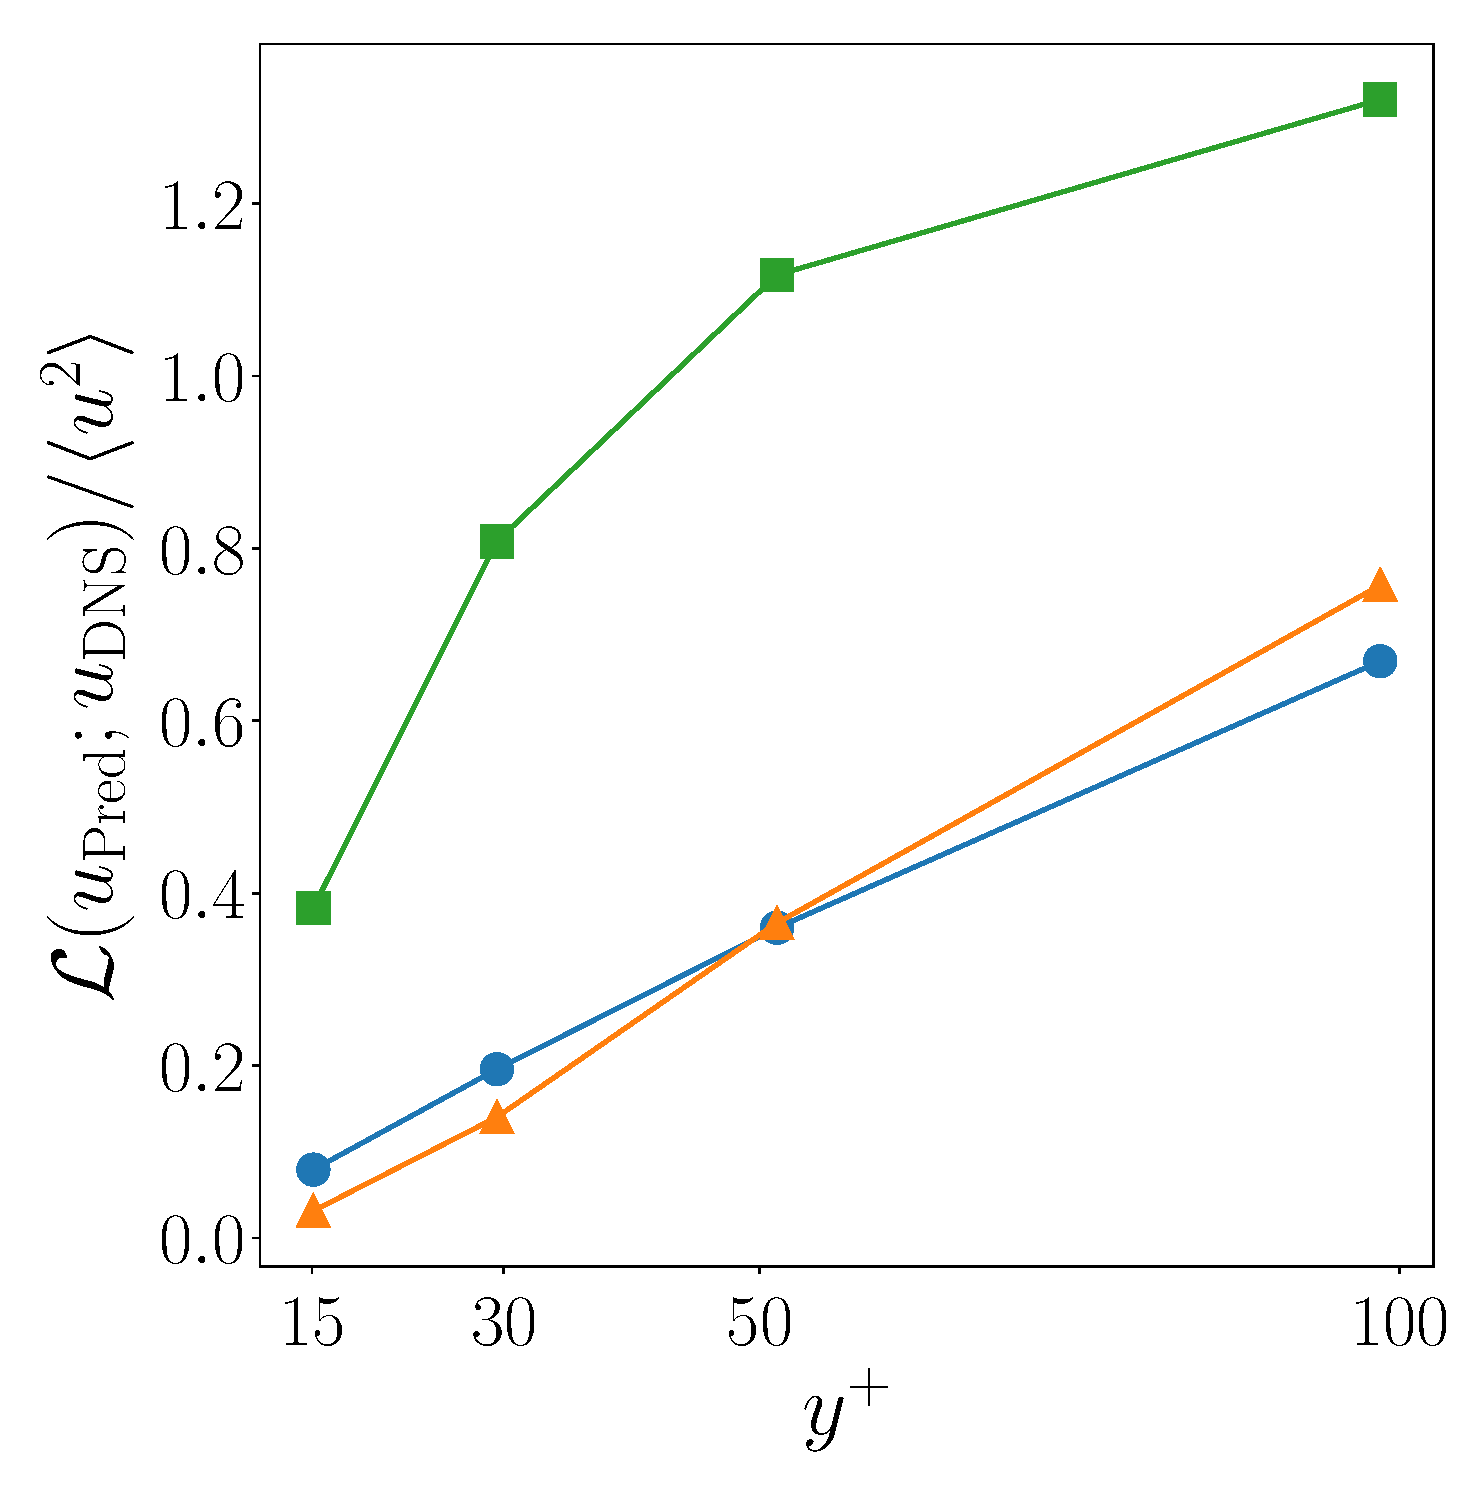
\includegraphics[width=.32\columnwidth]{Ret180/mse_u180_rms_scale.eps}
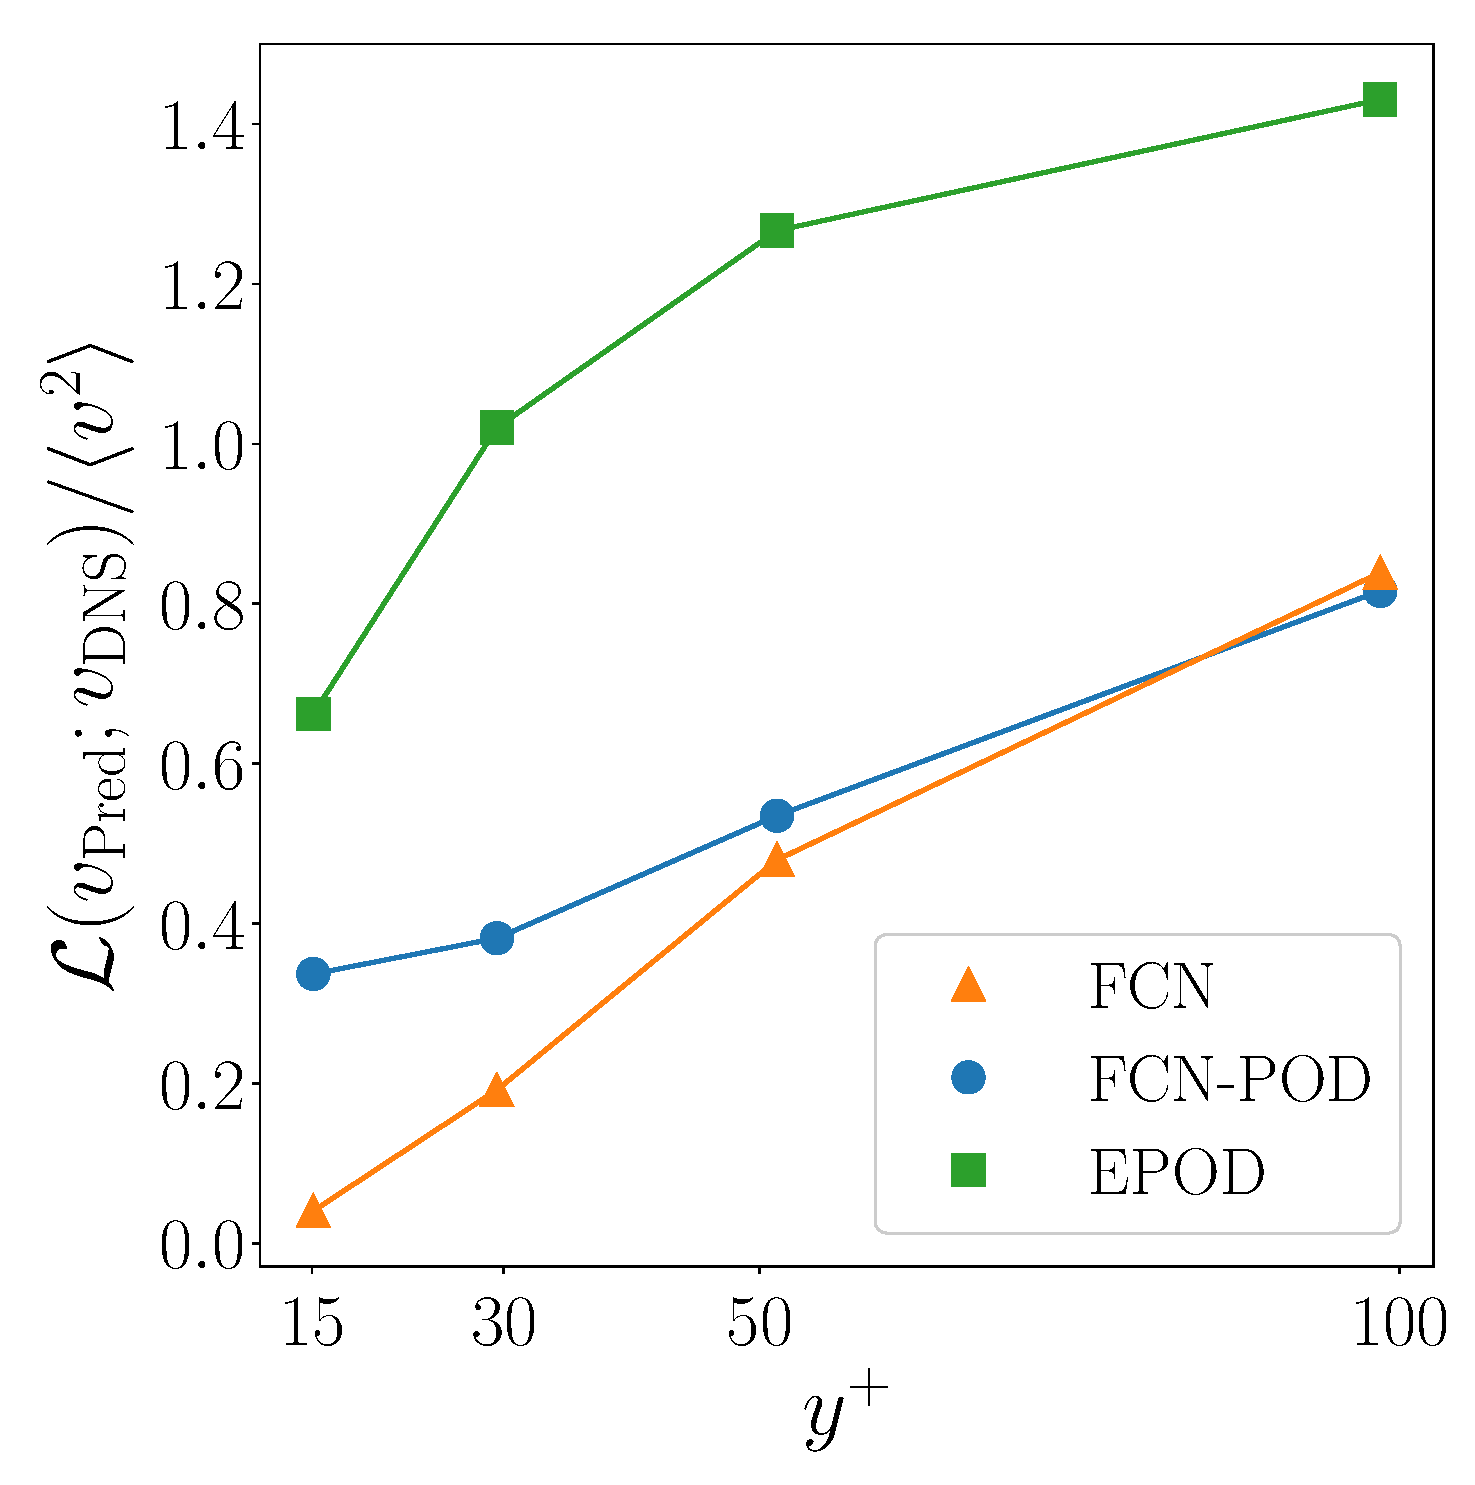
\includegraphics[width=.32\columnwidth]{Ret180/mse_v180_rms_scale.eps}
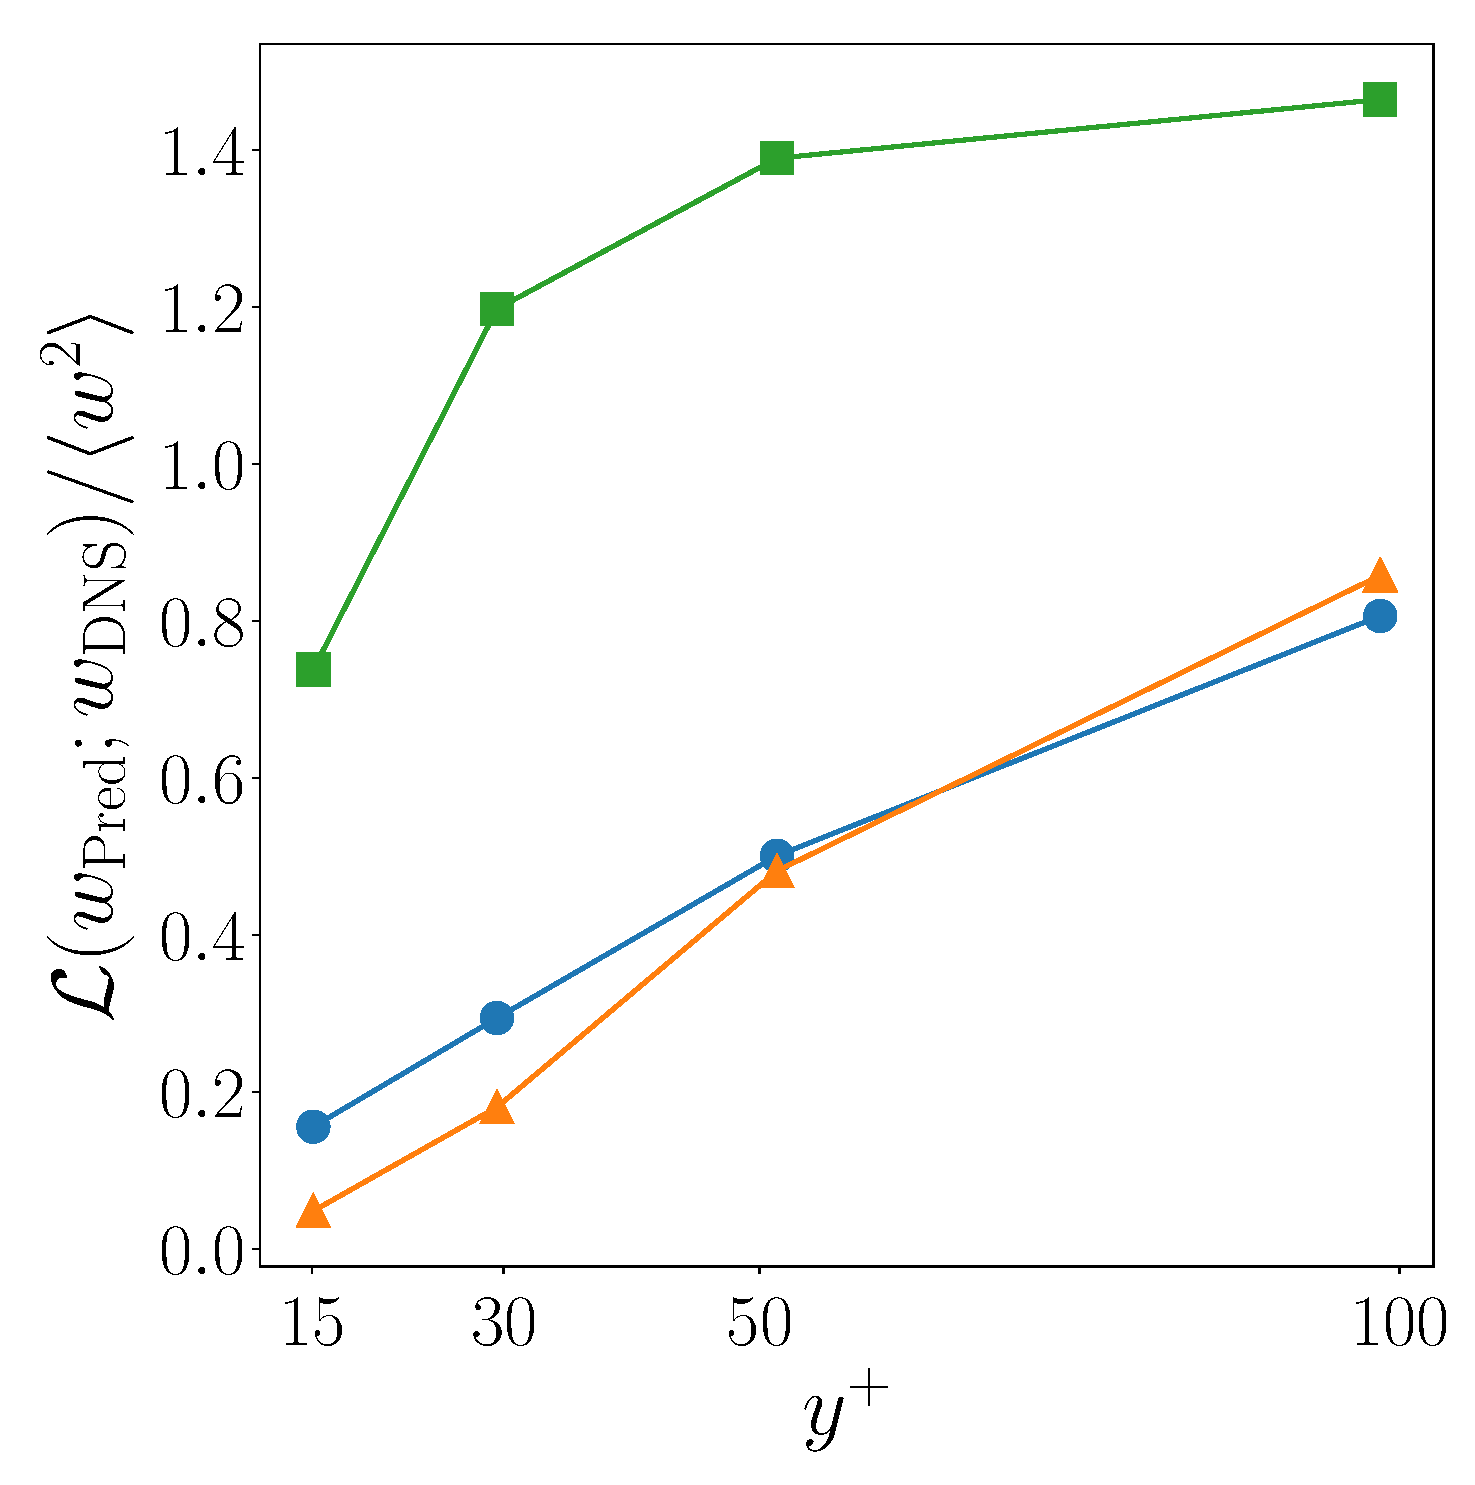
\includegraphics[width=.32\columnwidth]{Ret180/mse_w180_rms_scale.eps}
\end{center}
\caption{\label{fig:loss180} Mean-squared-error in the instantaneous fields (scaled with the corresponding RMS components) predicted by the three models at $Re_{\tau} = 180$, for the streamwise (left), wall-normal (middle) and spanwise (right) velocity fluctuations.}
\end{figure}

% Multiple component predictions
The FCN architecture reported by \citet{guastoni2020prediction} would only predict the streamwise velocity component of the velocity field at the target $y^+$.
The addition of the two other components implies that the FCN has multiple outputs that need to be optimized at the same time. We note that adding the two additional fluctuating components as outputs leads to slightly less accurate predictions with respect to those reported by \citet{guastoni2020prediction} for one single output.
This is not surprising, since the capacity of the network remained unchanged, however we tested a variation of the model architecture based on this observation, in order to have more layers dedicated to the prediction of each individual component.
This network variation has a common part, identical to the original FCN up to the 4$^{\text{th}}$ convolutional layer, in which the weights are optimized using the information from the error gradients computed for all the outputs.
The last two convolution operations are replicated for each velocity component and the weights of these layers are updated only with the error associated to the respective output.
Such a network, despite its higher capacity, provided worse predictions.
A strong causal relation between the different components of the velocity~\citep{lozano2020causality} can be a possible explanation for this result, which shows that updating all the weights with information from the three components at the same time can be beneficial for the quality of the predictions.
Note that it is not trivial to design an architecture able to provide the best trade-off between single-component predictions and usage of the information from all the components, and obtaining such an architecture would require further investigation.
For the FCN-POD model the multiple-component predictions were obtained as discussed by \citet{guemes2019sensing}.
The temporal POD coefficients can be projected on spatial POD modes involving the three velocity components, thus requiring only one output to predict the three fluctuations.
The network architecture is different than the one used by \citet{guemes2019sensing}, since it predicts directly all the needed time coefficients for each snapshot.
While the final fully-connected layer included in the network architecture by \citet{guemes2019sensing} improves the robustness of the prediction, the FCN-POD implementation used here has a much smaller number of weights, thus significantly reducing the computational cost, and retains a larger number of POD modes (and thus more energy).


\begin{figure}
\begin{center}
\includegraphics[width=\textwidth]{Ret550/u_550smaller_fields.png}
\end{center}
\caption{\label{fig:field_comp550} Comparison of the streamwise fluctuation fields at $Re_{\tau} = 550$, scaled with the corresponding $u_\mathrm{RMS}$, from EPOD (1$^{\text{st}}$ row), FCN-POD (2$^{\text{nd}}$ row), reference DNS (3$^{\text{rd}}$ row) and FCN (4$^{\text{th}}$ row). Results at $y^+=15$ (1$^{\text{st}}$ column), $y^+=30$ (2$^{\text{nd}}$ column), $y^+=50$ (3$^{\text{rd}}$ column) and $y^+=100$ (4$^{\text{th}}$ column).}%\highlight{AG: This instantaneous fields seem too positive (too red). LG: the mean of the field is not zero, but slightly positive, moreover the overall distribution of u in the dataset is skewed, it has positive mode.}% \highlight{LG: currently in draft mode otherwise it takes forever to load}}
\end{figure}

Predictions of the streamwise fluctuation fields from the various methods at $Re_{\tau} = 550$ are shown in figure~\ref{fig:field_comp550}, while the results for the wall-normal and spanwise components are presented in Appendix~\ref{appA}.
Despite the higher friction Reynolds number, the FCN maintains a performance similar to the one achieved for $Re_{\tau}=180$, at all wall-normal locations.
Note that the FCN has the same architecture as the lower-Reynolds-number case, {\it i.e.} it has the same number of trainable parameters, while in the case of the FCN-POD approach, the network was modified to reconstruct approximately the same amount of energy as at $Re_{\tau}=180$.
Despite the higher number of employed subdomains, the tiling is more apparent at $Re_{\tau}=550$.
The prediction performance of the FCN-POD model degrades less quickly than the FCN when moving away from the wall, however the latter still performs better at $y^+=50$, as shown in figure~\ref{fig:loss550}.
On the other hand, the EPOD also exhibits similar error levels as those reported for $Re_{\tau}=180$, except at $y^+=15$, where the reconstruction of the streamwise-fluctuation field is significantly worse.

\begin{figure}
\begin{center}
\includegraphics[width=.32\columnwidth]{Ret550/mse_u550_rms_scale.eps}
\includegraphics[width=.32\columnwidth]{Ret550/mse_v550_rms_scale.eps}
\includegraphics[width=.32\columnwidth]{Ret550/mse_w550_rms_scale.eps}
\end{center}
\caption{\label{fig:loss550} Mean-squared-error in the instantaneous fields (scaled with the corresponding RMS components) predicted by the three models at $Re_{\tau}=550$, for the streamwise (left), wall-normal (middle) and spanwise (right) velocity fluctuations.}
\end{figure}


\subsubsection{Inclination of coherent structures} \label{sss:shift}
The coherent structures in wall-bounded turbulence are inclined~\citep{marusic2007reynolds}, with a slope that can be computed by finding the maximum spatial correlation $\mathcal{R}_{ij}(\delta x)$ between the inputs at the wall (index $i$) and the outputs (index $j$), with $\delta x$ representing the distance in the streamwise direction at which the correlation is computed.
By including a streamwise \textit{shift} in the output fields, it is possible to obtain the maximum correlation at $\delta x=0$, ensuring that the footprint of the coherent structure is included in the receptive field of the output.
The use of such a shift was also discussed by \citet{sasaki2019transfer} in a similar context.
By considering the maximum correlation between the wall-shear stress in the streamwise direction and the streamwise velocity at a certain $y^+$, we obtain an angle:
\begin{equation}
 \theta_{\mathrm{shift}} = \tan^{-1}\left(\frac{\arg\,\max_{\delta x} R_{11}(\delta x)}{\delta y}\right) \approx 11^{\circ}
\end{equation}
\noindent at $Re_{\tau}=180$, where $\delta y$ indicates the considered distance from the wall.
 The obtained value is slightly lower than previous observations~\citep{marusic2007reynolds,sasaki2019transfer}, possibly because of the low Reynolds number.
 The inclusion of the shift information has been tested using two alternative implementations: first, by modifying the target output field, {\it i.e.} considering a field that has been sampled later in the simulation, although the accuracy of the introduced shift is limited by the value of the sampling period.
 The second approach makes use of the periodicity of the output fields, which are translated in the streamwise direction until the maximum correlation is obtained at $\delta x=0$.
 This approach allows to more accurately introduce the shift, however in this case the underlying hypothesis is that the shift is sufficiently small so that temporal dynamics modify the flow in a negligible manner.
 None of the two shift implementations provided the expected improvement, and we observed a significant degradation of the prediction performance.
 These results could possibly be explained by the fact that coherent structures of different size have different inclinations, and imposing a single value is detrimental for the overall network performance, despite having chosen the angle that provides the maximum spatial correlation.
 Furthermore, the quality of the predictions is measured using the MSE between the prediction and the reference: this error indicator considers all wavelengths at the same time, without considering how the different wavelengths are affected by the shift.
 Further investigation of this aspect, also at higher $Re_{\tau}$, will be conducted in future work.

\subsection{Predictions of turbulence statistics}\label{ss:stat}

By averaging over the fields obtained from the neural-network models and EPOD, it is possible to evaluate the turbulence statistics of the predicted flow.
First we consider the dataset at $Re_{\tau}=180$: the predicted RMS fluctuations of the three components are shown in figure~\ref{fig:stats180}, together with the reference DNS profiles.
The error in these statistical quantities is defined as:
%
\begin{equation}
    E_\mathrm{RMS}^+(u) = \frac{\left| u_\mathrm{RMS,Pred}^+ - u_\mathrm{RMS,DNS}^+ \right|}{u_\mathrm{RMS,DNS}^+},
\end{equation}
for the streamwise component, and similarly for the other two components.
As above, the subscripts `DNS' and `Pred' refer to the reference and predicted profiles, respectively.
An important premise is that neither of the neural-network-based models is explicitly optimized to reproduce the statistics of the original simulation.
This prevents the neural networks from learning only the average behaviour of the flow, however the predictions may be less statistically accurate, with the aim of maximizing the instantaneous performance.
Note that here we favor instantaneous performance because our motivation is to use non-intrusive sensing for closed-loop flow control.

The prediction errors in the various RMS profiles are summarized in table~\ref{tab:RMS_err_180}, and they are averaged over the different training runs for the FCN and FCN-POD models.
Note that the average is performed over the fluctuation-intensity values and not on the predictions, because that would alter the statistical properties of the predicted flow fields.
The comparison of the errors from the different models shows that the statistical performance mimics the one observed for the instantaneous predictions at $y^+=15$ and $y^+=30$, with the FCN performing better than the FCN-POD and EPOD models.
Furthermore, the FCN model provides a similar performance for the fluctuations of all three velocity components, while POD-based methods are more accurate in the predictions of $u_\mathrm{RMS}^+$.
This is related to the choice of not scaling the different velocity components in the FCN-POD and EPOD approaches, and the fact that near the wall the most energetic dynamics of the flow are in the streamwise direction.
Taking into account the standard deviation in the results of the neural-network-based methods, the three models provide similar error levels at $y^+=50$. At $y^+=100$ the scenario is opposite to what we observed close to the wall: the FCN exhibits the highest errors, while the EPOD provides the best results.
The error in the prediction of $u_\mathrm{RMS}^+$ from the FCN-POD model is between those of the two other models, while the wall-normal and spanwise intensities are closer to the errors from the FCN, due the reasons outlined above.

\begin{figure}
\begin{center}
\includegraphics[width=.32\columnwidth]{Ret180/uu180.eps}
\includegraphics[width=.32\columnwidth]{Ret180/vv180.eps}
\includegraphics[width=.32\columnwidth]{Ret180/ww180.eps}
\end{center}
\caption{\label{fig:stats180} Comparison between the DNS (\full) and the predictions of streamwise (left),
 wall-normal (middle) and spanwise (right) velocity
fluctuations at $Re_{\tau} = 180$.}
\end{figure}

\begin{table}
\centering
\resizebox{\columnwidth}{!}{%
    \begin{tabular}{l l*{4}{c}}
        $E_\mathrm{RMS}^+(\cdot)\ [\%]$ &         & $y^+=15$                       & $y^+=30$                     & $y^+=50$           & $y^+=100$          \\[0.3cm]

                                        & EPOD    & $\phantom{0}6.03~~~~~~~~~~~$   & $13.87~~~~~~~~~~~$           & $20.50~~~~~~~~~~~~$ & $25.15~~~~~~~~~~~~$ \\
        $u$                             & FCN     & $\phantom{0}1.16~(\pm 0.74)$   & $\phantom{0}6.79~(\pm 1.31)$ & $21.47~(\pm 1.97)~$ & $50.82~(\pm 2.19)~$ \\
                                        & FCN-POD & $\phantom{0}4.70~(\pm 0.02)$   & $10.70~(\pm 0.02)$           & $20.15~(\pm 0.03)~$ & $35.46~(\pm 0.02)~$ \\[0.3cm]

                                        & EPOD    & $11.68~~~~~~~~~~~$             & $18.89~~~~~~~~~~~$           & $23.97~~~~~~~~~~~~$ & $28.10~~~~~~~~~~~~$ \\
        $v$                             & FCN     & $\phantom{0}1.74~(\pm 1.00)$   & $10.18~(\pm 1.67)$           & $26.66~(\pm 0.76)~$ & $59.05~(\pm 1.61)~$ \\
                                        & FCN-POD & $20.29~(\pm 0.02)$             & $22.32~(\pm 0.02)$           & $31.32~(\pm 0.01)~$ & $51.48~(\pm 0.04)~$ \\[0.3cm]

                                        & EPOD    & $13.01~~~~~~~~~~~$             & $22.48~~~~~~~~~~~$           & $27.27~~~~~~~~~~~~$  & $28.72~~~~~~~~~~~~$ \\
        $w$                             & FCN     & $\phantom{0}2.79~(\pm 0.36)$   & $\phantom{0}9.65~(\pm 1.07)$ & $25.60~(\pm 1.214)$  & $59.59~(\pm 1.310)$ \\
                                        & FCN-POD & $\phantom{0}8.50~(\pm 0.04)$   & $15.95~(\pm 0.06)$           & $28.38~(\pm 0.004)$  & $47.42~(\pm 0.001)$ \\
    \end{tabular}%
    }
    \caption{Percentage error in the prediction of the various RMS fluctations at the different wall-normal locations. Results at $Re_{\tau} = 180$.}
    \label{tab:RMS_err_180}
\end{table}

The statistical analysis is repeated also for the models trained at $Re_{\tau} = 550$, with the predicted RMS fluctuations shown in figure~\ref{fig:stats550} and the relative error with respect to the reference simulation in table~\ref{tab:RMS_err_550}.
FCN-based models do not show a significant variation in the prediction of the streamwise fluctuations with respect to the results at $Re_{\tau}=180$, whereas the EPOD exhibits higher errors at this Reynolds number (also in the other two fluctuating components).
The FCN has a consistent behaviour also for the fluctuations in the \textit{y}- and \textit{z}-directions, however the FCN-POD performs slightly worse than before, following the same trend but with higher error levels.
The FCN-POD method outperforms the FCN approach only at $y^+=100$, confirming the results of the instantaneous performance at $Re_{\tau} = 550$.

\begin{figure}
\begin{center}
\includegraphics[width=.32\columnwidth]{Ret550/uu550_v3.eps}
\includegraphics[width=.32\columnwidth]{Ret550/vv550_v3.eps}
\includegraphics[width=.32\columnwidth]{Ret550/ww550_v3.eps}
\end{center}
\caption{\label{fig:stats550} Comparison between the DNS (\full) and the predictions of streamwise (left),
 wall-normal (middle) and spanwise (right) velocity
fluctuations at $Re_{\tau} = 550$.}
\end{figure}

\begin{table}
\centering
\resizebox{\columnwidth}{!}{%
    \begin{tabular}{l l*{4}{c}}
        $E_\mathrm{RMS}^+(\cdot)\ [\%]$ &         & $y^+=15$                  & $y^+=30$                     & $y^+=50$                      & $y^+=100$          \\[0.3cm]

                                     & EPOD    & $49.69~~~~~~~~~~$            & $48.53~~~~~~~~~~~$           & $47.62~~~~~~~~~~~$            & $46.53~~~~~~~~~~~$ \\
        $u$                          & FCN     & $0.98~(\pm 0.66)$            & $\phantom{0}8.10~(\pm 0.62)$ & $15.33~(\pm 0.22)$            & $33.06~(\pm 0.30)$ \\
                                     & FCN-POD & $7.53~(\pm 0.27)$            & $15.53~(\pm 0.39)$           & $20.75~(\pm 0.85)$            & $26.79~(\pm 0.36)$ \\[0.3cm]

                                     & EPOD    & $51.57~~~~~~~~~~$            & $49.13~~~~~~~~~~~$           & $48.13~~~~~~~~~~~$            & $48.07~~~~~~~~~~~$ \\
        $v$                          & FCN     & $\phantom{0}1.74~(\pm 0.11)$ & $11.21~(\pm 1.41)$           & $24.20~(\pm 1.38)$            & $50.82~(\pm 0.26)$ \\
                                     & FCN-POD & $30.73~(\pm 0.06)$           & $35.20~(\pm 0.09)$           & $41.75~(\pm 0.10)$            & $53.04~(\pm 0.18)$ \\[0.3cm]

                                     & EPOD    & $51.56~~~~~~~~~~$            & $50.35~~~~~~~~~~~$           & $49.42~~~~~~~~~~~$            & $49.08~~~~~~~~~~~$ \\
        $w$                          & FCN     & $\phantom{0}1.86~(\pm 0.60)$ & $\phantom{0}9.03~(\pm 0.31)$ & $21.21~(\pm 1.27)$            & $51.83~(\pm 0.38)$ \\
                                     & FCN-POD & $15.74~(\pm 0.05)$           & $23.63~(\pm 0.07)$           & $31.97~(\pm 0.10)$            & $48.20~(\pm 0.24)$ \\
    \end{tabular}%
    }
    \caption{Percentage error in the prediction of the various RMS fluctations at the different wall-normal locations. Results at $Re_{\tau}=550$.}
    \label{tab:RMS_err_550}
\end{table}

\subsection{Predictions of power-spectral density}\label{ss:spec}
\begin{figure}
    \centerline{\includegraphics[width=384pt]{Ret180/spectra_re180large.pdf}}
    \caption{Pre-multiplied two-dimensional power-spectral densities for $Re_{\tau}=180$. The contour levels contain 10\%, 50\% and 90\% of the maximum DNS power-spectral density. Shaded contours refer to the reference data, while contour lines refer to \lcap{.-}{fcn} FCN, \lcap{--}{FCN-POD} FCN-POD and \lcap{:}{epod} EPOD predictions, respectively.}
    \label{fig:spectra180}
\end{figure}

The energetic scales present in the predicted fields, as well as their associated energy, are compared with those in the reference DNS data through spectral analysis.
In figure~\ref{fig:spectra180} we show the pre-multiplied two-dimensional power-spectral density of the streamwise, wall-normal and spanwise fluctuations (denoted by $\phi_{uu}$, $\phi_{vv}$ and $\phi_{ww}$ respectively) at $Re_{\tau}=180$, where $\lambda_{x}$ and $\lambda_{z}$ denote the streamwise and spanwise wavelengths, whereas $k_{x}$ and $k_{z}$ are the corresponding wavenumbers.
These results confirm the observations made in $\S$\ref{ss:inst}: at $y^+=15$, all the considered models are able to correctly predict the energy content of the flow at all wavelengths, with the FCN slightly outperforming the two POD-based approaches.
Note that the FCN-POD model is able to reconstruct the energy content of the flow at wavelengths that are longer than the size of the subdomains, proving that this is not a limiting factor for the model.
However, a small jump, probably due to a lack of smoothness at the edges of the subdomains, can be observed in the streamwise wavelength for the 10\%-energy level in the wall-normal and spanwise components.
These jumps are found at a wavelength $\lambda_x^+ \approx 180$, corresponding to the subdomain size.
At $y^+=30$ there is a slight energy attenuation which becomes increasingly more noticeable when the predicted flow is farther away from the wall.
At $y^+=100$ the POD-based methods perform better than the FCN model, a fact that can be explained by considering two concurring aspects: the first is that POD methods only predict the temporal dynamics of the system, thus the overall energy-scale distribution stored in the POD spatial modes does not need to be predicted.
This allows to reconstruct more than $50\%$ of the flow fields, at least in the streamwise component.
The second aspect is the fact that the receptive field from the FCN method, while sufficient for planes closer to the wall, is not large enough to reproduce the large scales present at larger $y^{+}$.

Figure~\ref{fig:spectra550} reports the reference and predicted power-spectral densities at $Re_{\tau}=550$.
As opposed to what was observed for the instantaneous predictions and the turbulence statistics, the spectra highlight the differences and similarities between the models used for the two Reynolds numbers.
As noted above, the FCN architecture is the same for both $Re_{\tau}$, however this implies that the receptive field is smaller at higher Reynolds number when it is measured in outer units.
This can potentially help in the prediction of the small scales, but it can also be detrimental for the larger scales.
Note that the different size of the receptive field does not seem to affect the predicted energy content of the FCN, which shows the same trends as for the low-$Re_{\tau}$ case.
On the other hand, the spectra of the FCN-POD with $12\times12$ subdomains (the same amount as in the low-$Re_{\tau}$ case, not shown) exhibits spurious periodic peaks due to the tiling.
This observation motivated the increased number of subdomains considered at $Re_{\tau}=550$.
As in the low-$Re_{\tau}$ case, the FCN-POD approach is able to reconstruct the scales larger than the subdomain size, but the countour line exhibits a small jump in the streamwise wavelength for the 10\%-energy level.
This jump appears at a wavelength $\lambda_x^+ \approx 200$, corresponding to the subdomain size employed in the high-$Re_{\tau}$ case.
This jump is also appreciated in the streamwise component at $y^+=15$.
The POD-based approaches are outperformed by the FCN in the range of $y^+=15-50$.
Farther from the wall, the accuracy of the FCN is matched by the FCN-POD method. It is interesting to note that the EPOD does not follow the same attenuation process as the FCN-based methods in the wall-normal and spanwise components.
As one moves farther from the wall, the FCN-based methods fail to reproduce a wider range of small scales, whereas the EPOD exhibits more difficulties predicting the large scales.
When it comes to the spectral peaks far from the wall, while the FCN-based methods produce noisier predictions than in the low-$Re_{\tau}$ case, the EPOD is not able to reproduce that part of the spectra.

\begin{figure}
    \centerline{\includegraphics[width=384pt]{Ret550/spectra_re550large.pdf}}
    \caption{Pre-multiplied two-dimensional power-spectral densities for $Re_{\tau}=550$. The contour levels contain 10\%, 50\% and 90\% of the maximum DNS power-spectral density. Shaded contours refer to the reference data, while contour lines refer to \lcap{.-}{fcn} FCN, \lcap{--}{FCN-POD} FCN-POD and \lcap{:}{epod} EPOD predictions, respectively.}
    \label{fig:spectra550}
\end{figure}

\section{Transfer learning}\label{ss:tl}

A number of more advanced techniques have also started to be adopted from the specialized machine-learning literature and applied to fluid-dynamics research.
One notable example is \textit{transfer learning}~\citep{pan2009survey}, a method that allows to transfer knowledge from one neural-network model to another one, thus reducing the amount data and time required for training.
\citet{guastoni2020prediction} showed that the training time at a given wall-normal location may be significantly reduced if the network parameters are initialized using the optimized parameters of a previously-trained network at another wall-normal location.
Similarly, \citet{kim2020prediction} used the convolutional network trained at a low Reynolds number to predict the flow at a higher Reynolds number.

Transfer learning represents an appealing solution for the main drawback of neural networks, which is the need to train them with a sufficient amount of data.
Training typically requires specialized hardware and in our specific application the computational cost of generating the training and test datasets is not negligible.
Furthermore, this cost grows as $Re_{\tau}$ increases, making the generation of training data through DNS unfeasible at the Reynolds numbers that are relevant for engineering applications.
In this regard, it is important to make an efficient use of the data and the trained models at our disposal.
In this work, the possibility of transferring knowledge between models trained at different friction Reynolds numbers is investigated.
At a fixed wall-normal distance, the weights of the FCN model trained on the dataset at $Re_{\tau} = 180$ are loaded before training the network with the higher-$Re_{\tau}$ dataset.
This is possible because the network has the same amount of trainable parameters in both cases, as noted above.
The learning rate is the only parameter that needs to be modified: a lower value has to be set, in order to prevent the optimizer from diverging too quickly from the weight configuration used for initialization.
While in \citet{guastoni2020prediction} we froze the first layers of the initialized network because the input was the same at the different wall-normal locations, in this case all the layers are trainable because the input distribution changes from one $Re_{\tau}$ to the other one.

The transfer-learning numerical experiments that follow are designed with two objectives in mind.
First, we investigate the effect of using the parameters of previously-trained model to initialize a model that will be trained at a different target $Re_{\tau}$ than the first model.
Second, we verify whether the non-random initialization that we described can potentially improve the training process, reducing the amount of data at higher $Re_{\tau}$ that is needed to achieve the same performance of a model trained from scratch, using the entire training/validation dataset, as we did in section~\ref{ss:results}.
To this end, we initialized a FCN model with the parameters learnt on the $Re_{\tau}=180$ dataset and we trained such model on the full training/validation datasets at $Re_{\tau}=550$.
Subsequently, the same initialization is used for models that are trained on a reduced dataset at $Re_{\tau}=550$, namely 25\% and 50\% of the full dataset.
Differently from the previous sections, only one training run was performed for each case.
In order to compare models trained with datasets of different sizes, we considered the number of weight updates through the optimization algorithm during training.
In figure~\ref{fig:transfer} the validation and test losses are compared for the models trained with the full dataset and a random initialization.
When the initialized model is trained on the full dataset, the performance is consistently better than that of the random initialization, both in terms of validation and test loss.
The improvement is more evident close to the wall, whereas at $y^+=100$ the two models provide approximately the same results after the first 150,000 updates.
Transferring knowledge between different Reynolds numbers is then not only feasible, but also advantageous in terms of performance when the same amount of data is considered.
Note that we kept the same ratio (4:1) when dividing training and validation sets even when the size of the dataset was reduced.
In particular, when 50\% or 25\% of the samples are used, the validation set becomes too small to provide a reliable estimate of the error.
On the other hand, the size of the test dataset is the same as the previous experiments.
Up to $y^+=50$, the initialized networks are able to provide a performance that is very similar to that of the reference model with the same number of updates, with significant savings in terms of amount of data needed to train the network.
On the other hand, at $y^+=100$ a sufficient number of samples becomes a necessary condition to ensure the convergence to an optimal configuration: the loss of the network trained with 50\% of the training dataset does not improve after the first 100,000 updates, while with 25\% of the original dataset the network exhibits overfitting.
The initialized models are able to provide a comparable accuracy also from the statistical point of view, as reported in table~\ref{tab:RMS_err_transfer}.
We stress once again that the networks are not explicitly optimized to reduce the error in the statistics and that small variations in these error figures can be ascribed to the stochastic nature of the optimization algorithm.
Overall, these results demonstrate the feasibility of knowledge transfer from models at different $Re_{\tau}$: with careful tuning of the hyperparameters it should be possible to substantially reduce the training time, as well as the amount of data needed for training.
Although not tested, the transfer between different wall-normal locations described in~\citet{guastoni2020prediction} is still applicable in this case, thus enabling a more efficient prediction of the flow at different wall-normal locations.
\begin{figure}
    \centerline{\includegraphics[width=\textwidth]{transfer_learning_v4.eps}}
    \caption{Validation (\full) and test (\dashed) loss in the FCN prediction at (from left to right, top to bottom): $y^+=15$, 30, 50 and 100. Orange represents the models trained with the full dataset and random initialization, grey the models trained with the full dataset and initialized with previously-trained networks, pink and brown represent models initialized with the parameters from the $Re_{\tau}=180$ network, trained with 50\% and 25\% of the original dataset, respectively.}
    \label{fig:transfer}
\end{figure}

\begin{table}
\centering
\resizebox{\columnwidth}{!}{%
    \begin{tabular}{l l*{4}{c}}
        $E_\mathrm{RMS}^+(\cdot)\ [\%]$ &          & $y^+=15$                    & $y^+=30$                     & $y^+=50$                      & $y^+=100$                    \\[0.3cm]

        $u$                             & Ref.     & $0.98~(\pm 0.66)$           & $8.10~(\pm 0.62)$            & $15.33~(\pm 0.22)$            & $33.06~(\pm 0.30)$           \\
                                        & 100\%    & $1.22\phantom{~(\pm 0.00)}$ & $7.15\phantom{~(\pm 0.00)}$  & $16.09\phantom{~(\pm 0.00)}$  & $32.75\phantom{~(\pm 0.00)}$ \\
                                        & 50\%     & $2.94\phantom{~(\pm 0.00)}$ & $7.11\phantom{~(\pm 0.00)}$  & $16.33\phantom{~(\pm 0.00)}$  & $34.11\phantom{~(\pm 0.00)}$ \\
                                        & 25\%     & $1.15\phantom{~(\pm 0.00)}$ & $7.74\phantom{~(\pm 0.00)}$  & $14.78\phantom{~(\pm 0.00)}$  & $33.78\phantom{~(\pm 0.00)}$ \\[0.3cm]

        $v$                             & Ref.     & $1.74~(\pm 0.11)$           & $11.21~(\pm 1.41)$           & $24.20~(\pm 1.38)$            & $50.82~(\pm 0.26)$           \\
                                        & 100\%    & $1.86\phantom{~(\pm 0.00)}$ & $9.40\phantom{0~(\pm 0.00)}$ & $24.40\phantom{~(\pm 0.00)}$  & $51.59\phantom{~(\pm 0.00)}$ \\
                                        & 50\%     & $2.40\phantom{~(\pm 0.00)}$ & $9.46\phantom{0~(\pm 0.00)}$ & $25.96\phantom{~(\pm 0.00)}$  & $50.90\phantom{~(\pm 0.00)}$ \\
                                        & 25\%     & $1.71\phantom{~(\pm 0.00)}$ & $11.33\phantom{~(\pm 0.00)}$ & $23.15\phantom{~(\pm 0.00)}$  & $50.43\phantom{~(\pm 0.00)}$ \\[0.3cm]

        $w$                             & Ref.     & $1.86~(\pm 0.60)$           & $9.03~(\pm 0.31)$            & $21.21~(\pm 1.27)$            & $51.83~(\pm 0.38)$           \\
                                        & 100\%    & $1.75\phantom{~(\pm 0.00)}$ & $8.65\phantom{~(\pm 0.00)}$  & $21.05\phantom{~(\pm 0.00)}$  & $53.04\phantom{~(\pm 0.00)}$ \\
                                        & 50\%     & $2.61\phantom{~(\pm 0.00)}$ & $7.70\phantom{~(\pm 0.00)}$  & $21.34\phantom{~(\pm 0.00)}$  & $52.60\phantom{~(\pm 0.00)}$ \\
                                        & 25\%     & $1.22\phantom{~(\pm 0.00)}$ & $9.67\phantom{~(\pm 0.00)}$  & $20.35\phantom{~(\pm 0.00)}$  & $49.75\phantom{~(\pm 0.00)}$ \\
    \end{tabular}%
    }
    \caption{Percentage error in the prediction of the various RMS fluctations at the different wall-normal locations from models initialized with parameters from the $Re_{\tau}=180$ FCN. The statistics of the different initialized models are computed after 250,000 updates, and they are shown together the models with full dataset and random initialization, which is included as a reference. Results at $Re_{\tau}=550$.}
    \label{tab:RMS_err_transfer}
\end{table}

\section{Conclusions}\label{ss:conclu}

In this work, we introduced and compared two different models based on fully-convolutional neural networks, for prediction of the velocity fluctuations at a given wall-normal distance, using quantities measured at the wall as inputs.
The FCN and FCN-POD models are improved versions of previous architectures, used by \citet{guastoni2020prediction} and \citet{guemes2019sensing}, respectively.
Both of them are able to provide predictions in very good agreement with the reference data, simulated by means of the pseudo-spectral DNS code SIMSON~\citep{chevalier2007pseudo}, up to $y^{+}=50$.
Such an agreement is verified by comparing the error in instantaneous predictions, turbulence statistics (namely RMS fluctuations) and the energy content at the different wavelengths ({\it i.e.} spectral analysis).
Both models show better prediction capabilities than EPOD (which is a linear method) in almost all the wall-normal locations and investigated features, thanks to their ability to predict nonlinear scale interactions.
Furthermore, we showed that these architectures can be used at two different friction Reynolds numbers ($Re_{\tau}=180$ and 550) with minimal modifications, providing satisfactory results on both datasets.

The two models are designed under the assumption that local information at the wall is sufficient to predict the flow farther away, however the FCN-POD model partially encodes further physical information of the system by using the spatial modes obtained through POD of the training dataset.
On the other hand, features like the periodicity of the flow are enforced in the FCN by exploiting the mathematical characteristics of the model.
These architectural differences are associated with performance discrepancies at the tested wall-normal locations: the FCN provides higher accuracy than the FCN-POD model closer to the wall, {\it i.e.} up to $y^+=30$ at $Re_{\tau} = 180$ and up to $y^+=50$ at $Re_{\tau} = 550$.
Farther from the wall, the FCN-POD method produces the most accurate predictions.
The choice between these two models is motivated by the application into which the prediction model is integrated.

Despite the encouraging results discussed here, both models can be improved in terms of network architecture and training.
An attempt to embed further physical information into the FCN did not result in improved predictions, as reported in $\S$\ref{sss:shift}.
The correct way of incorporating this information to enhance the predictions is an active area of research. As another example, the high-frequency noise in the FCN predictions could be reduced with appropriate filtering, possibly adding a trainable layer to the network to perform this operation.
The FCN-POD model has a higher number of hyperparameters to be set, such as the number of predicted temporal modes or the size of the subdomains.
A more thorough inspection of the hyperparameter space may provide a significant improvement in the prediction performance.
Differently from the FCN, in the FCN-POD model the velocity components are not scaled to have the same magnitude: such a modification could help to predict the wall-normal and spanwise components of the velocity more accurately, even though it would also modify the POD mode sorting because of the different energy norm.
Furthermore, the FCN-POD results exhibit lack of smoothness at the subdomain edges in the flow predictions.
Finally, both models are trained to minimize a loss function based on the instantaneous error.
Such a function could be modified to improve other physical characteristics of the predicted flow, for example the turbulence statistics and the spectral energy content.

To reduce the training time in view of industrial applications, the implementation of transfer learning was tested for the FCN model.
Transfer learning can exploit a network trained at a lower Reynolds number to provide the weight initialization for training at a higher Reynolds number, thus reducing the requirements in terms of training time and data.
The results are very encouraging, showing that it is possible to train the network with 50\% and even 25\% of the original training dataset, obtaining a performance similar to that of the reference model up to $y^{+}=50$.

Once the neural networks are trained, they are computationally cheap to evaluate, and they can become even cheaper by \textit{pruning} the parts that have a negligible contribution to the final result off the network.
Such an operation is not possible \textit{a priori}, since the training determines how the inputs have to be processed to obtain the output.
By reducing the computational cost of the evaluation it is possible to deploy the model using low-powered hardware and/or potentially run it in real-time.
Thus, the proposed FCN-based methods could be used for non-intrusive sensing of the flow, which is needed for closed-loop control applications.
Furthermore, since the FCN models are able to reproduce non-linear interactions in wall-bounded turbulence, new promising avenues in turbulence research could be opened by the network interpretation~\citep{fan2020interpretability}, as shown by \citet{iten2020discovering}, who demonstrated that neural networks can provide relevant physical insights.

\section*{Acknowledgements}
All the codes employed in this work will be released as open-source on GitHub upon publication in the peer-reviewed literature.
The authors acknowledge the funding provided by the Swedish e-Science Research Centre (SeRC), the G\"oran Gustafsson Foundation and the Knut and Alice Wallenberg (KAW) Foundation.
The numerical simulations were carried out on resources provided by the Swedish National Infrastructure for Computing (SNIC) at PDC and HPC2N.
Part of this study was conducted in the context of the 4th Madrid Turbulence Workshop, in the context of the COTURB project (Coherent Structures in Wall-bounded Turbulence), funded by the European Research Council (ERC), under grant ERC-2014.AdG-669505. S
D and AI were partially supported by the Grant DPI2016-79401-R funded by the Spanish State Research Agency (SRA) and European Regional Development Fund (ERDF).

\section*{Declaration of Interests}
The authors report no conflict of interest.

\appendix
\section{}\label{app:training}
%\rev{LG: Add details regarding FCN-POD}
This Appendix contains the training details of the neural network models in the FCN and FCN-POD method. Both models introduced in section~\ref{s:methodology} need to be tuned to perform optimally on the chosen dataset.
The networks were trained using the Adam~\citep{kingma2014adam} optimization algorithm for 50 epochs, with a scheduled exponential learning-rate decay.
We used the optimizer hyperparameters suggested in the original paper, except the $\hat{\epsilon}$ parameter that was set to 0.1 following TensorFlow recommendations~\citep{abadi2016tensorflow}.
The total number of trainable parameters in the FCN is 1,264,131 and it does not depend on the $Re_{\tau}$ of the dataset.
On the other hand, this number is $Re_{\tau}$-dependent for the FCN-POD model, as the number of subdomains and reconstructed POD modes changes.
For the $Re_{\tau}=180$ case the number of trainable parameters is 4,733,248, while for the $Re_{\tau}=550$ case it is 5,028,224.

For the FCN model the $Re_{\tau}=180$ dataset, composed by input and output fields, has a size of about 70 GB per wall-normal distance, while the $Re_{\tau}=550$ dataset occupies 120 GB.
Depending on the amount of available RAM it might not be possible to load the entire dataset in memory, however our implementation does not require to load it at once, allowing training on less-performing computer as well.
The training was performed on two different GPUs, namely NVIDIA K80 and NVIDIA RTX2080Ti.
The former has 24 GB of GPU memory, whereas the latter only 12 GB.
The turbulent field snapshots have a comparatively high resolution with respect to the samples used in image processing and the GPU memory can also be a limiting parameter.
For a given dataset, the amount of memory that is allocated on the GPU depend on the batch size, that is the number of samples used to estimate the loss function gradient at each update of the learnable parameters of the network.
In the $Re_{\tau}=550$, the batch size is limited to 2 samples when the faster RTX2080Ti is used. With this setting the gradient approximation might be too noisy and the training performance might be degraded, therefore we suggest to use at least a batch size of 4, using two RTX2080Ti GPUs.

Due to the reduced-order nature of FCN-POD method, the size of the training/validation datasets is lower: 40 GB for $Re_{\tau}=180$ dataset and 70 GB for $Re_{\tau}=550$ dataset.
Thanks to the max pooling operations that are not present in the FCN model, the size of the tensors allocated on GPU is smaller and this allows to train the model with a batch size of 8 for both datasets.

\section{}\label{appA}
This Appendix contains the wall-normal and spanwise fluctuations corresponding to the fields shown in figures~\ref{fig:field_comp180} and~\ref{fig:field_comp550} for $Re_{\tau}=180$ and 550, respectively.
If we observe the wall-normal fluctuations at $Re_{\tau}=180$ in figure~\ref{fig:field_comp180v}, the FCN model provides better predictions than POD-based methods at $y^+=15$.
The tiling of the subdomains is more apparent in the FCN-POD predictions, while the EPOD predictions contain small features that are not present in the DNS reference field.
Similar observations can be made at $y^+=30$.
As we move farther away from the wall, at $y^+=50$, the accuracy of the neural-network-based models is similar.
For the FCN-POD the flow features in the streamwise direction appear smoothed out with respect to the DNS fields; on the other hand the same features have more jagged edges in the FCN predictions, possibly as a consequence of the localized nature of the predictions.
As observed for the streamwise velocity fluctuations, the performance degrades as we move farther away from the wall.
Note that some features are completely missing in the EPOD predictions, due to the fact that the three velocity components are predicted at the same time.
From the observation of the spanwise fluctuations predictions, the behaviour of the three methods is similar to the one in the wall-normal components.
Note however that, closer to the wall, the FCN-POD provides more accurate predictions for the spanwise fluctuation component than for the wall-normal component, as it can be observed in figure~\ref{fig:loss180}.

\begin{figure}
\begin{center}
\includegraphics[width=\textwidth]{Ret180/v_180smaller_labels.png}
\end{center}
\caption{\label{fig:field_comp180v} Comparison of the wall-normal fluctuation fields at $Re_{\tau} = 180$, scaled with the corresponding $v_\mathrm{RMS}$, from EPOD (1$^{\text{st}}$ row), FCN-POD (2$^{\text{nd}}$ row), reference DNS (3$^{\text{rd}}$ row) and FCN (4$^{\text{th}}$ row). Results at $y^+=15$ (1$^{\text{st}}$ column), $y^+=30$ (2$^{\text{nd}}$ column), $y^+=50$ (3$^{\text{rd}}$ column) and $y^+=100$ (4$^{\text{th}}$ column).}
\end{figure}

\begin{figure}
\begin{center}
\includegraphics[width=\textwidth]{Ret180/w_180smaller_labels.png}
\end{center}
\caption{\label{fig:field_comp180w} Comparison of the spanwise fluctuation fields at $Re_{\tau} = 180$, scaled with the corresponding $w_\mathrm{RMS}$, from EPOD (1$^{\text{st}}$ row), FCN-POD (2$^{\text{nd}}$ row), reference DNS (3$^{\text{rd}}$ row) and FCN (4$^{\text{th}}$ row). Results at $y^+=15$ (1$^{\text{st}}$ column), $y^+=30$ (2$^{\text{nd}}$ column), $y^+=50$ (3$^{\text{rd}}$ column) and $y^+=100$ (4$^{\text{th}}$ column).}
\end{figure}

When a higher Reynolds number is considered, the error trends of the neural-network-based models in figure~\ref{fig:loss550} are comparable to the one observed at $Re_{\tau}=180$, for the wall-normal and spanwise fluctuations.
On the other hand, the EPOD predictions improve when moving from $y^+=15$ to $y^+=30$, before the performance starts degrading as we move farther from the wall.
Additionally, figures~\ref{fig:field_comp550v} and~\ref{fig:field_comp550w} show that, close to the wall, the intensity of the fluctuations in the wall-normal and spanwise direction is significantly underestimated by the POD-based methods, when compared to FCN.
As the wall-normal distance increases, the fluctuations range predicted by the FCN reduces as well and at $y^+=100$ the range is comparable for all three methods.

\begin{figure}
\begin{center}
\includegraphics[width=\textwidth]{Ret550/v_550smaller_fields.png}
\end{center}
\caption{\label{fig:field_comp550v} Comparison of the wall-normal fluctuation fields at $Re_{\tau} = 550$, scaled with the corresponding $v_\mathrm{RMS}$, from EPOD (1$^{\text{st}}$ row), FCN-POD (2$^{\text{nd}}$ row), reference DNS (3$^{\text{rd}}$ row) and FCN (4$^{\text{th}}$ row). Results at $y^+=15$ (1$^{\text{st}}$ column), $y^+=30$ (2$^{\text{nd}}$ column), $y^+=50$ (3$^{\text{rd}}$ column) and $y^+=100$ (4$^{\text{th}}$ column).}
\end{figure}

\begin{figure}
\begin{center}
% \centering
% \input{images/test.pdf_tex}
 \includegraphics[width=\textwidth]{Ret550/w_550smaller_fields.png}
 \end{center}
\caption{\label{fig:field_comp550w} Comparison of the spanwise fluctuation  fields at $Re_{\tau} = 550$, scaled with the corresponding $w_\mathrm{RMS}$, from EPOD (1$^{\text{st}}$ row), FCN-POD (2$^{\text{nd}}$ row), reference DNS (3$^{\text{rd}}$ row) and FCN (4$^{\text{th}}$ row). Results at $y^+=15$ (1$^{\text{st}}$ column), $y^+=30$ (2$^{\text{nd}}$ column), $y^+=50$ (3$^{\text{rd}}$ column) and $y^+=100$ (4$^{\text{th}}$ column).}
\end{figure}


%\begin{footnotesize}
%\bibliography{scigenbibfile.Donald+Duck.Mickey+Mouse.Goofy+G.+Goof}\bibliographystyle{acm}
%\end{footnotesize}
%
%\end{document}



%------------------------------------------------------------------------------
% Bibliography
%------------------------------------------------------------------------------
%
%\clearpage
\bibliographystyle{jfm}
\bibliography{thesis}
%
\IfFileExists{paper2/paper.bbl}{%------------------------------------------------------------------------------
% Define title, author(s), affiliation and publishing status
%
\papertitle[Wall-bounded turbulence from wall quantities] % Short title used in healines (optional)
{%
Convolutional-network models to predict wall-bounded turbulence from wall quantities% THE COMMENT SYMBOL AT THE END OF THIS LINE IS NEEDED
}%
%
\papertoctitle{Wall-bounded turbulence from wall quantities} % Title for toc
%
\paperauthor[L. Guastoni \etal] % Short authors used in headlines and List Of Papers
{%
  Luca Guastoni$^{1,2}$, Alejandro Güemes$^3$, Andrea Ianiro$^3$, Stefano Discetti$^3$, Phillip Schlatter$^{1,2}$, Hossein Azizpour$^{4,2}$ and Ricardo Vinuesa$^{1,2}$%
}%
%
\listpaperauthor{Guastoni, L., Güemes, A., Ianiro, A., Discetti, S., Schlatter, P., Azizpour, H. \& Vinuesa, R.}% (optional) Short authors used in List Of Papers
%
\paperaffiliation
{%
  $^1$ Linn\'e FLOW Centre, KTH Mechanics, S-100 44 Stockholm, Sweden\\%
  $^2$ Swedish e-Science Research Centre (SeRC), Stockholm, Sweden\\%
  $^3$ Aerospace Research Group, Universidad Carlos III de Madrid, Leganés, Spain\\%
  $^4$ Division of Robotics, Perception and Learning, KTH Royal Institute of Technology, Stockholm, Sweeden\\
}%
%
\paperjournal[J. Fluid Mech., \textbf{Under review}] % Short publish info used in List Of Papers
{%
	Journal of Fluid Mechanics, \textbf{Under review}%
}%
%
\papervolume{}%
%
%\papernumber{1}
%
\paperpages{}%
%
\paperyear{2021}%
%
\papersummary%
{% Insert summary of the paper here (used in introduction)
Two models based on convolutional neural networks are trained to predict the two-dimensional instantaneous velocity-fluctuation fields at different wall-normal locations in a turbulent open-channel flow, using the wall-shear-stress components and the wall pressure as inputs.
The first model is a fully-convolutional neural network (FCN) which directly predicts the fluctuations, while the second one reconstructs the flow fields using a linear combination of orthonormal basis functions, obtained through proper orthogonal decomposition (POD), hence named FCN-POD.
Both models are trained using data from direct numerical simulations (DNS) at friction Reynolds numbers $Re_{\tau} = 180$ and 550.
Being able to predict the nonlinear interactions in the flow, both models show better predictions than the extended proper orthogonal decomposition (EPOD), which establishes a linear relation between input and output fields.
The performance of the models is compared based on predictions of the instantaneous fluctuation fields, turbulence statistics and power-spectral densities.
FCN exhibits the best predictions closer to the wall, whereas FCN-POD provides better predictions at larger wall-normal distances.
We also assessed the feasibility of transfer learning for the FCN model, using the model parameters learned from $Re_{\tau}=180$ dataset to initialize those of the model that is trained on the $Re_{\tau}=550$ dataset.
After training the initialized model at the new $Re_{\tau}$, our results indicate the possibility to match the reference-model performance up to $y^{+}=50$, with $50\%$ and $25\%$ of the original training data.
We expect that these non-intrusive sensing models will play an important role in applications related to closed-loop control of wall-bounded turbulence.
}
%
\graphicspath{{paper2/}}%
%
%
%===============================================================================
%                            BEGIN PAPER
%===============================================================================
%
\begin{paper}

\makepapertitle

%------------------------------------------------------------------------------
% Abstract
%------------------------------------------------------------------------------
%
\begin{paperabstract}
	Two models based on convolutional neural networks are trained to predict the two-dimensional velocity-fluctuation fields at different wall-normal locations in a turbulent-open channel flow, using the wall-shear-stress components and the wall pressure as inputs.
	The first model is a fully-convolutional neural network (FCN) which directly predicts the fluctuations, while the second one reconstructs the flow fields using a linear combination of orthonormal basis functions, obtained through proper orthogonal decomposition(POD), hence named FCN-POD.
	Both models are trained using data from two direct numerical simulations (DNS) at friction Reynolds numbers $Re_{\tau} = 180$ and 550.
	Thanks to their ability to predict the nonlinear interactions in the flow, both models show a better prediction  performance  than  the  extended  proper  orthogonal  decomposition  (EPOD), which establishes a linear relation between input and output fields.
	The performance of the various models is compared based on predictions of the instantaneous fluctuation fields, turbulence statistics and power-spectral densities.
	The FCN exhibits the best predictions closer to the wall, whereas the FCN-POD model provides better predictions at larger wall-normal distances.
	We also assessed the feasibility of performing transfer learning for the FCN model, using the weights from $Re_{\tau} = 180$ to initialize those of the $Re_{\tau} = 550$ case. Our results indicate that it is possible to obtain a performance similar to that of the reference model up to $y^+= 50$, with 50\% and 25\% of the original training data.
	These non-intrusive sensing models will play an important role in applications related to closed-loop control of wall-bounded turbulence
        \keywords{turbulent flows, turbulence simulation}
\end{paperabstract}


%------------------------------------------------------------------------------
% Article
%------------------------------------------------------------------------------
%
%\documentclass[12pt, twocolumn]{article}
%\usepackage{helvet}
%
%\usepackage{epsfig}
%\usepackage[latin1]{inputenc}
%\begin{document}
%
%\title{Emulating Von Neumann Machines and Massive Multiplayer Online Role-
%Playing Games}
%\author{Mickey Mouse, Goofy G. Goof and Donald Duck}
%
%\date{}

%\maketitle




%\section*{Abstract}
%
% Many computational biologists would agree that, had it not been for
% Byzantine fault tolerance, the synthesis of replication that made
% developing and possibly investigating erasure coding a reality might
% never have occurred. In this work, we prove  the synthesis of linked
% lists. Even though such a hypothesis at first glance seems
% counterintuitive, it always conflicts with the need to provide
% object-oriented languages to systems engineers. APER, our new framework
% for mobile archetypes, is the solution to all of these grand
% challenges.




\section{Introduction}

In this work, we assess the potential of deep neural networks~\cite[DNNs, see][]{lecun2015deep} to perform {\it non-intrusive sensing}, that consists in using measurable quantities in a fluid flow to reconstruct its behaviour in another location in the domain or to predict its dynamics in the future, without using probes that affect the flow itself.
For instance, it is possible to accurately measure time-resolved quantities at the wall, such as the wall-shear stress or the pressure, and then correlate these measurements with the flow farther away.
A reliable flow estimation is typically a prerequisite for closed-loop control applications, where the actuation is applied with the aim of suppressing the effect of certain structures in the flow~\citep{choi1994active}.
In order to effectively perform closed-loop control it is necessary to monitor the instantaneous state of the flow so as to devise the best way to affect it, however characterizing the flow state can be extremely challenging, particularly at very high Reynolds numbers where the near-wall structures become progressively smaller.

Before the appearance of DNNs, flow-field predictions were performed mainly through linear methods.
Among them, the linear stochastic estimation (LSE) introduced by \citet{adrian1988stochastic} stands out.
Recently \citet{suzuki2017estimation} and \citet{encinar2019logarithmic} have used LSE to reconstruct the velocity field on a wall-parallel plane in a turbulent channel flow employing wall measurements.
The latter study showed that LSE can only reconstruct the large wall-attached eddies in the outer part of the logarithmic region.
An extension of the LSE method in the spectral domain~\citep{tinney2006spectral} was shown to be more suitable for noisy predictions in turbulent flows.
More recently \citet{baars2014proper} proposed a method based on proper orthogonal decomposition (POD) to improve the spectral-LSE approach. \citet{boree2003extended} reported the possibility of projecting a synchronized field on the POD temporal modes of another quantity; this method is known as extended POD (EPOD).
The correlation matrix between the temporal POD coefficients of two given quantities can be used to predict one based on the other.
The work of \citet{boree2003extended} proved EPOD to be equivalent to LSE when all modes are retained in the reconstruction.
Using remote probes, EPOD has been used to provide predictions in turbulent jets~\citep{tinney2008low}, channel flows~\citep{discetti2018estimation}, pipe flows~\citep{discetti2019characterization} and wall-mounted obstacles~\citep{hosseini2016modal, bourgeois2013generalized}.
Note however that in the latter work quadratic terms are included in the model of the POD coefficient dynamics, hinting at the need of non-linear estimation even for a relatively-simple, predominantly-oscillatory flow.
In this regard, \citet{sasaki2019transfer} recently assessed the capabilities of both linear and non-linear transfer functions with single and multiple inputs to provide turbulent-flow predictions.
They documented a significant improvement in the predictions when the transfer functions were designed to account for nonlinear interactions between the inputs and the flow field.
The improved prediction capabilities of nonlinear methods over linear ones were also reported by \citet{mokhasi2009predictive} and \citet{nair2020leveraging}.

DNNs are non-linear models that have found application in many research areas~\citep{jean2016combining,de2018clinically,norouzzadeh2018automatically,ham2019deep,udrescu2020ai,vinuesa2020role}.
Due to their potential applications in flow modelling, identification of turbulence features and flow control, DNNs have recently received extensive attention in the fluid-mechanics research community~\citep{kutz2017deep,jimenez2018machine,duraisamy2019turbulence,brunton2020machine}.
Here we provide a brief overview of the recent neural network applications in fluid mechanics, before coming back to the flow estimation problem we investigated in this work.
In the case of turbulence modelling, DNNs have been reported to improve the results of Reynolds-averaged Navier--Stokes~\cite[RANS, ][]{ling2016reynolds,wu2017priori} models and large-eddy simulations~\cite[LES, ][]{maulik2019subgrid,lapeyre2019training,beck2019deep}.
There are also a number of on-going efforts towards including the constraints from the Navier--Stokes equations into prediction models through the so-called physics-informed neural networks~\citep{wang2017physics,raissi2019physics}.
Furthermore, several artificial-intelligence-based solutions have been proposed to perform optimal control on different types of flows, such as the wake behind one or more cylinders~\citep{rabault2019artificial,raibaudo2020machine}.
Other promising applications of machine learning to fluid mechanics include generation of inflow conditions~\citep{fukami2019synthetic} and extraction of flow patterns~\citep{raissi2020hidden}.

DNNs have also been used in temporal prediction of dynamical systems.
As an example, \citet{srinivasan2019predictions} compared the capabilities of the multi-layer perceptron (MLP, also known as fully-connected-layer neural network) and several long-short-term memory (LSTM) networks to predict the coefficients of a low-order model for near-wall turbulence~\citep{moehlis2004low}.
While the most relevant flow features are captured by both architectures, the LSTM network outperformed the MLP in terms of ability to predict turbulence statistics and the dynamics of the flow.
This work has been extended by \citet{eivazi2020recurrent}, where the LSTM network has been compared with a Koopman-based framework which accounts for non-linearities through external forcing.
Although both approaches provide accurate predictions of the dynamical evolution of the system, the latter outperforms the LSTM in terms of time and data required for training.
Similar temporal predictions of the near-wall model~\citep{moehlis2004low} were conducted by \cite{pandey2020perspective} using echo state networks (ESN).
Moreover, nonlinear autoregressive exogeneous networks (NARXs) have been used by \citet{lozano2020causality} to exploit the relation between the temporal dynamics of the Fourier coefficients of a minimal turbulent channel flow.
Their results showed accurate predictions of the bursting events in the logarithmic layer from buffer-region data.
Other related work, in the context of control of the Kuramoto--Sivashinsky (KS) chaotic system, was recently conducted by \cite{bucci2019control}.
Note however that the use of temporal sequences implies a high computational cost to generate well-resolved temporal data.
Furthermore, longer sequences require higher memory requirements in order to predict the future behaviour.
For these reasons, several neural-network-based models that learn spatial relations have been proposed in the literature.
Convolutional neural networks (CNNs) have become increasingly popular during the last years due to the hierarchical structure of their input~\citep{fukushima1980neocognitron,fukushima1988neocognitron, lecun1989backpropagation,lecun1998gradient}.
For instance, \citet{fukami2019super,fukami2021machine} have shown that flow fields from the laminar wake of a cylinder and a turbulent channel can be reconstructed from extremely coarse data with remarkable success.
CNNs have also been used to investigate the dynamical features of the flow without \textit{a-priori} knowledge, as shown by \citet{jagodinski2020uncovering}.

Neural networks are mathematical models which exhibit very appealing properties, such as being \textit{universal approximators}~\citep{hornik1989multilayer}.
This means that they can potentially represent any continuous function with the adequate model parametrization, even though there is no guarantee that it is possible to infer the value of the parameters from data sampled from the original function.
Nonetheless, neural-network parameters are typically tuned through data-driven training, and as such they have been compared and used together with other data-driven methods.
For instance, the relationship between proper orthogonal decomposition~\cite[POD, see][]{lumley1967structure} and the MLP is well documented in the literature~\citep{bourlard1988auto,baldi1989neural}.
These works showed that a MLP with a single hidden layer is equivalent to POD if a linear activation function is used.
One of the early applications on a fluid-dynamics dataset was proposed by \citet{milano2002neural}, who compared the results of POD-based neural networks with linear and non-linear functions for the prediction of near-wall velocity fields, showing that nonlinear POD has significantly better predictive capabilities.
More recently, the emergence of autoencoder architectures has motivated a renewed interest in the application of neural networks for dimensionality reduction.
\citet{hinton2006reducing} proposed the use of deep autoencoders to obtain a low-order representation of high-dimensional data, showing that this approach is able to retain more information than POD.
It is interesting to note that this work avoids the inherent difficulty of optimizing weights in deep autoencoders by training each layer with a Restricted Boltzmann Machine.
\citet{murata2020nonlinear} used an autoencoder with convolutional layers to obtain a low-order representation of the flow around a cylinder.
Their results suggest that CNN autoencoders with linear activation functions reproduce the same dimensionality reduction as POD, while the use of nonlinear activation functions improves the reconstruction performance.
On a related note, flow reconstruction based on shallow neural networks was studied by \cite{erichson2020shallow} in several fluid-mechanics examples.

This work is not the first in which neural networks are used to perform non-intrusive sensing in wall-bounded flows: in a seminal study over 20 years ago, \cite{lee1997application} tested a two-layer neural network (with a single non-linear activation function) to predict the wall actuation, based on the wall-shear-stress components, in order to reduce the drag at the wall.
\citet{inigo2014dynamic} predicted the velocity field in a transitional boundary-layer flow using wall-shear measurements, by projecting the velocity fields on a POD basis and using a dynamic observer to predict the dynamics of the flow.
More recently, \citet{kim2020prediction} used the two wall-shear-stress rcomponents to predict the instantaneous wall-normal heat flux  with satisfactory results.
The same wall information was used by \citet{guastoni2020prediction} to predict the instantaneous streamwise flow fields at several wall-normal positions using convolutional networks.
Their results show that these neural networks provide better predictions than linear methods (see below) in terms of instantaneous predictions and second-order statistics.
The predictions were limited to one velocity component and to a low Reynolds number. In this work, all the velocity components are predicted and a higher $Re$ is investigated as well.
Furthermore, in the work by \citet{guemes2019sensing} the information of the most-energetic scales was encoded into a POD basis, and a CNN was used to predict that information at different wall-normal locations from streamwise wall-shear-stress measurements.
Their results demonstrated that CNNs can significantly outperform linear methods in the prediction of POD time coefficients for low-order reconstruction of the velocity fields.
Their convolutional network would predict only one POD temporal coefficient at a time, in this work all the coefficients are computed at the same time thanks to the implementation of an improved network architecture.

DNNs perform best when training and test data are taken from the same distribution, {\it i.e.} for the same flow and at the same Reynolds number in our case.
However, in  a real-world application the flow conditions will be continuously varying and/or it might be unfeasible to perform a full training at exactly the same conditions.
If the flow behaviour at the Reynolds number of interest is roughly the same as the training Reynolds number and if the neural network can successfully approximate it, then the model should be able to perform consistently across the different Reynolds numbers, as shown in active flow control applications by~\citet{tang2020robust}.
In order to improve the performance at a different Reynolds number, it would then be possible to exploit initial training at a certain flow condition and transfer this knowledge to another one.
Such knowledge transfer could reduce significantly the amount of data needed for training and improve the network applicability for industrial applications.
Transfer learning~\citep{pan2009survey} is the suitable learning framework to address this issue, and it is discussed in detail below.

The methods proposed by \citet{guastoni2020prediction} and \citet{guemes2019sensing}, henceforth referred to as fully-convolutional network (FCN) and FCN-POD respectively, are extended in the present study.
Both models are able to provide a nonlinear characterization of the relation between wall features and the flow on wall-parallel planes.
The purpose of this work is to provide a detailed comparison of the two aforementioned nonlinear methods regarding their capabilities to predict turbulent flow fields from wall information.
Their improvement over linear methods is measured using EPOD as a reference. Furthermore, transfer learning was applied to the FCN approach  with the purpose of evaluating to what extent a network trained at one Reynolds number can be used at a different one.

The remainder of this article is organised as follows.
Section \ref{datasets} describes the numerical databases used for training and testing the neural networks and $\S$\ref{meth} provides a brief comparison between the considered models.
The FCN and FCN-POD methods are further detailed in $\S$\ref{ss:FCN} and $\S$\ref{ss:FCN-POD} respectively, while EPOD is discussed in $\S$\ref{ss:epod}.
Results from the considered prediction methods are presented and compared in $\S$\ref{ss:results}, including instantaneous fields in $\S$\ref{ss:inst}, second-order statistics in $\S$\ref{ss:stat}, and spectra in $\S$\ref{ss:spec}.
Furthermore, an assessment of transfer learning between different Reynolds numbers is presented in $\S$\ref{ss:tl}.
Finally, the main conclusions of the work are presented in $\S$\ref{ss:conclu}.
Two Appendices are provided containing additional information about the training of the neural-network-based models and regarding the predicted instantaneous flow fields.

\section{Methodology}\label{s:methodology}
\subsection{Datasets}\label{datasets}
All the DNN variants in this study have been trained using the data generated from direct numerical simulations (DNS) of a turbulent open-channel flow.
Periodic boundary conditions are imposed in the \textit{x-} and \textit{z-}directions (which are the streamwise and spanwise coordinates, respectively), and a no-slip condition is applied at the lower boundary ($y=0$, where $y$ is the wall-normal coordinate).
Differently from a standard channel-flow simulation, a symmetry condition is imposed at the upper boundary.
In standard channel flows, the wall-attached coherent structures may extend beyond the channel centerline, thus affecting the other wall~\citep{lozano2012three}.
On the other hand, in open-channel flows there is no upper wall.
This makes the simulation more suitable to investigate to which extent the neural networks are able to learn the dynamics of near-wall turbulence, since the interaction of the large scales with both walls is not present.

The simulation is performed using the pseudo-spectral code SIMSON~\citep{chevalier2007pseudo} with constant mass flow rate, in a domain $\Omega = L_x \times L_y \times L_z = 4\pi h \times h \times 2\pi h$ (where $h$ is the channel height), as shown in figure~\ref{channel}.
Two friction Reynolds numbers $Re_{\tau}$ (based on $h$ and the friction velocity $u_{\tau}=\sqrt{\tau_w/\rho}$, where $\tau_w$ is the wall-shear stress and $\rho$ is the fluid density) are considered, as summarized in table~\ref{tab:dns}. The flow field is represented with $N_y$ Chebyshev modes in the wall-normal direction and with $N_x$ and $N_z$ Fourier modes in the streamwise and spanwise directions, respectively.
The instantaneous fields are obtained at constant time intervals from the time-advancing scheme, which is a second-order Crank--Nicholson scheme for the linear terms and a third-order Runge--Kutta method for the nonlinear terms.
Dealiasing using a standard 3/2 rule is employed in the wall-parallel Fourier directions.
The velocity fields to be used as ground truth for training and testing are sampled at the following inner-scaled wall-normal coordinates: $y^{+}=15,~30,~50$ and $100$.
Note that '+' denotes viscous scaling, {\it i.e.} in terms of the friction velocity $u_{\tau}$ or the viscous length $\ell^{*}=\nu / u_{\tau}$ (where $\nu$ is the fluid kinematic viscosity).
A dataset is defined as a collection of samples, each consisting of the shear-stress and pressure fields at the wall as inputs, along with the corresponding velocity fields at the target wall-normal locations as outputs.
The training/validation dataset at $Re_{\tau} = 180$ consists of 50,400 instantaneous fields, with a sampling period of $\Delta t^+_{s} = 5.08$.
The sampling period at $Re_{\tau} = 550$ is set to $\Delta t^+_{s} = 1.49$ and the training/validation dataset includes 19,920 fields.
The resolution in viscous units of the individual fields is the same in both $Re_{\tau}$ datasets.
This is necessary to represent all the flow features; however this also implies that the number of Fourier modes in the wall-parallel directions is higher at $Re_{\tau}=550$, as shown in table~\ref{tab:dns}, even if the domain $\Omega$ is the same.
A higher number of modes corresponds to a higher number of spatial locations in which the different quantities are sampled from the DNS and this partially compensate the lower number of fields since the two proposed methods act locally on the input data, as it will be shown in $\S$\ref{meth}.

In both $Re_{\tau}$ cases, the dataset is split into training and validation sets, with a ratio of 4:1. The training and validation sets are obtained from a group of randomly-initialized simulations.
With the number of samples chosen for our investigation at either $Re_{\tau}$, there is a simulation whose samples are used both for training or for validation.
Note that there is no temporal overlapping between the two datasets, as the first samples from the "shared" simulation are sequentially added to the training set until the required number of training samples is reached.
The remaining samples are then added to the validation set.
This is done to reduce the correlation between the two datasets.
While using the separate groups of simulations or adding an additional time separation between the last sample of the training set and the first sample of the validation would have further reduced the correlation, this was not enforced, since the validation error is only used during training to tune the network hyperparameters and avoid over-fitting the training dataset.
If the training provides satisfactory results, it is common practice to use both training and validation sets for the training of the final models.
This was not implemented in our case, but it allows the model to make use of all the available data to improve its performance.
The validation error may be significantly different from the one computed during testing, hence all the comparisons in this work are based on the error computed on the test dataset.
\begin{figure}
\begin{center}
\begin{overpic}[width=0.75\textwidth]{channel_flow_domain_nolabels.eps}
 \put (5,55) {flow}
 \put (22,17) {$L_x$}
 \put (73,12) {$L_z$}
 \put (87,32) {$L_y$}
 \put (87.5,16.5) {$y,v$}
 \put (94,5) {$x,u$}
 \put (76,2) {$z,w$}
\end{overpic}
\end{center}
\caption{\label{channel}Computational domain and frame of reference for the DNS of the turbulent open channel considered in this study.}
\end{figure}
The predictions used to assess the performance of the trained models were obtained from additional simulations.
This is done both at $Re_{\tau} = 180$ and $Re_{\tau} = 550$, and it is necessary to ensure that the training and test datasets are completely uncorrelated, both in space and time.
Test samples were taken from simulations initialized with a random seed, different from that of the training-data simulation.
The correlation between train simulations and between train and test simulations was checked with the cross-correlations $\rho_{ij}(h)$, defined as~\citep{makarashvili2017performance}:
\begin{equation}
    \rho_{ij}(h) = \frac{\gamma_{ij}(h)}{\sqrt{\gamma_{i}(0)\gamma_{j}(0)}},
\end{equation}
\noindent where $h$ is the time lag and $\gamma_{ij}(h)=\mathbb{E}[(x_{i,t+h}-\mu_i)(x_{j,t}-\mu_j)]$ are the cross-covariances. $i$ and $j$ refer to the two simulations and $x$ is the considered quantity, in this case one of the velocity components at a given wall-normal location.
By computing $\rho_{ij}(0)$, it was possible to verify that the simulations had run sufficiently long to ensure that they are overall stastistically uncorrelated, before starting the sampling to build the datasets.

The size of the test dataset (more than 3,000 fields for both $Re_{\tau}$) is sufficient to achieve convergence of the turbulence statistics from the predicted flow, and then these are compared  with the reference values from the DNS.
% \begin{table}
% \begin{center}
%     \begin{tabular}{l*{8}{c}}
%         $Re_{\tau}$ & $N_x \times N_z \times N_y$           & \vtop{\setbox0\hbox{\strut $\#$Train.+Val.}\copy0\hbox to\wd0{\hss\strut fields\hss}} & $\Delta t^+_{s,\mathrm{train}}$ & $T^+_{train}$ &$\#$Test fields & $\Delta t^+_{s,\mathrm{test}}$ & $T^+_{test}$ \\[0.4cm]
%
%         180         & $192 \times 192 \times 65\phantom{0}$ & 50,400                 & 5.08                            & $\approx 2.56\times 10^5$       & 3,125                & 1.69 & $\approx 5.3\times 10^3$ \\
%         550         & $512 \times 512 \times 193$           & 19,920                 & 1.49                            & $\approx 2.97\times 10^4$       & 3,320                & 1.49 & $\approx 5\phantom{.3}\times 10^3$ \\
%
%     \end{tabular}
%     \caption{Description of the DNS datasets used for computing the EPOD and training/testing the CNN-based models.}
%     \label{tab:dns}
% \end{center}
% \end{table}
  \begin{table}
  \centering
  \resizebox{\columnwidth}{!}{%
      \begin{tabular}{l*{8}{c}}
          $Re_{\tau}$ & $N_x \times N_z \times N_y$           & \vtop{\setbox0\hbox{\strut $\#$Train.+Val.}\copy0\hbox to\wd0{\hss\strut fields\hss}} & $\Delta t^+_{s,\mathrm{train}}$ & $T^+_{train}$ &$\#$Test fields & $\Delta t^+_{s,\mathrm{test}}$ & $T^+_{test}$ \\[0.4cm]

          180         & $192 \times 192 \times 65\phantom{0}$ & 50,400                 & 5.08                            & $\approx 2.56\times 10^5$       & 3,125                & 1.69 & $\approx 5.3\times 10^3$ \\
          550         & $512 \times 512 \times 193$           & 19,920                 & 1.49                            & $\approx 2.97\times 10^4$       & 3,320                & 1.49 & $\approx 5\phantom{.3}\times 10^3$ \\

      \end{tabular}%
      }
      \caption{Description of the DNS datasets used for computing the EPOD and training/testing the CNN-based models.}
      \label{tab:dns}
  \end{table}

\subsection{Summary of the methods}\label{meth}
In this study we consider three different data-driven methods to estimate the instantaneous two-dimensional fields of the velocity fluctuations, at a given wall-normal distance.
Two models (FCN and FCN-POD) are introduced and compared with the Extended POD method, which is used as a baseline model, highlighting the capabilities (and limitations) of linear estimation.
Despite using the same input data and predicting the same output quantities, the three models leverage on different tools in order to extract the information from the inputs and estimate the outputs.
Here we briefly review the differences and similarities between the models, each method is described in detail in the dedicated sections.

EPOD and FCN-POD use proper orthogonal decomposition~\cite[POD, see][]{lumley1967structure}: this approach is advantageous as it allows to filter out the noise content represented by small and uncorrelated scales, thus taking advantage of the energy optimality of POD modes.
Additionally, spatial and temporal dynamics are separated.
EPOD decomposes both the input and the output: the flow field at a certain wall-normal distance is reconstructed as a linear combination of orthogonal modes $\boldsymbol{\phi}_i(\boldsymbol{x})$:
\begin{equation}
    \boldsymbol{u}(\boldsymbol{x},t) \approx \sum^{N_m}_{i=1}\psi_i(t)\sigma_i\boldsymbol{\phi}_i(\boldsymbol{x}),
    \label{eq:decom}
\end{equation}
\noindent where $N_m$ is the total number of POD modes, $\psi_i(t)$ is the temporal POD coefficient corresponding to mode $i$, and $\sigma_i$ is its corresponding root-squared energy contribution.
While the orthogonal modes are computed from a POD of the training dataset, the temporal coefficients are estimated by decomposing input wall quantities using POD and assuming a linear correlation between the known temporal modes of the wall quantities $\psi_{w,i}(t)$ and the temporal modes $\psi_i(t)$ of the output flow field of the test dataset. F
urther details are provided in $\S$\ref{ss:epod}.
On the other hand, FCN-POD applies POD only on the output flow fields, using the spatial modes from the training set and predicting the corresponding temporal coefficients using a neural network.
This is a development of the model used by \citet{guemes2019sensing}, note however that in that study the domain employed and reconstructed provided a compact POD eigenspectrum, here the availability of a larger domain in the streamwise and spanwise directions spreads the energy content over a wider set of POD modes.
This makes the predictions of temporal coefficients more difficult, especially those associated with the least energetic modes.
To address this issue, the large instantaneous flow fields were subdivided into $N_{s_x}\times N_{s_z}$ smaller regions (henceforth referred to as subdomains).
The neural network predicts the temporal coefficients for all subdomains at the same time.

The FCN and FCN-POD models consider the instantaneous two-dimensional fields of the streamwise and spanwise wall-shear-stress components and of the wall pressure as inputs.
In the physical-coordinates representation of these fields, the presence of coherent features motivates the use of convolutional layers in our neural-network models to process the information.
In these layers, the inputs are processed at the same time, hence a convolution in three dimensions is performed and it is defined as:
\begin{equation}
    F_{i,j} = \sum_l \sum_m \sum_n I_{i-m,j-n,l}K_{m,n,l},
\end{equation}
\noindent following~\cite{goodfellow2016deep}, where $\mathbf{I} \in \mathbb{R}^{d_1 \times d_2 \times d_3}$ is the input, $\mathbf{K} \in \mathbb{R}^{k_1 \times k_2 \times k_3}$ is the so-called \textit{kernel} (or \textit{filter}) containing the learnable parameters of the layer, and the transformed output $\mathbf{F}$ is the \textit{feature map}.
Note that we consider $d_3 = k_3$, meaning that the resulting feature map is two-dimensional.
Multiple feature maps can be stacked and sequentially fed into another convolutional layer as input.
This allows the next layer to combine the features individually identified in each feature map, enabling the prediction of larger and more complex features for progressively deeper convolutional networks.
Note that a convolutional layer can be rewritten as a matrix multiplication, hence it is mathematically equivalent to a fully-connected layer~\cite{wei2017equivalence}.
If we assume that the input features are spatially localized, using a convolutional layer allows translational equivariance to be enforced in both periodic directions.
Furthermore, since $k_i \ll d_i\ \forall i\neq 3$, the use of kernels greatly reduces the number of parameters that need to be learned during training (in comparison with fully-connected MLP networks).

Both neural-network-based models use fully-convolutional neural network (hence FCN in the names).
This architecture is similar, but conceptually different from CNNs, which typically have several convolutional layers followed by one or more fully-connected layers (which are the building blocks of MLP networks).
In CNNs, the localized information processed by the individual convolutional kernels is combined to obtain a global prediction, whereas in FCNs only convolutional layers are present and the network architecture is based on the assumption that the relation between input and output variables is spatially localized.
The input region from which a single point of the output can draw information is called \textit{receptive field} and it can be computed based on the network architecture, as described by~\citet{dumoulin2016guide}.
In the FCN model, the instantaneous two-dimensional velocity fluctuations are directly predicted from the input fields by using the fully-convolutional neural network.
Additional details are provided in $\S$\ref{ss:FCN}.
On the other hand, the neural network in the FCN-POD model predicts the temporal coefficients for each of the $N_{s_x}\times N_{s_z}$ subdomains, as described in $\S$\ref{ss:FCN-POD}.

\subsection{Extended POD}\label{ss:epod}
EPOD provides a linear relation between input and output and it is the reference method for all the following comparisons.
Doing so, it is possible to assess the prediction improvement with nonlinear, neural-network-based methods in the context of wall-bounded turbulence.
Wall quantities in each field can be rearranged as a row vector and used to assemble a snapshot matrix $\mathbf{W}$. Using the method proposed by \citet{sirovich1987turbulence}, it is possible to decompose this matrix into POD modes as:
\begin{equation}
    \mathbf{W}=\boldsymbol{\Psi}_w\boldsymbol{\Sigma}_w\boldsymbol{\Phi}_w,
    \label{wpod0}
\end{equation}
\noindent with $\boldsymbol{\Psi}_w$ and $\boldsymbol{\Phi}_w$ being the temporal and spatial mode matrices respectively, and $\boldsymbol{\Sigma}_w$ being a diagonal matrix containing the singular values.
The extended POD modes~\citep{boree2003extended}, corresponding to the projection of the wall quantities on the flow-field temporal basis, are defined as
\begin{equation}
    \mathbf{L}=\boldsymbol{\Psi}_w^T\mathbf{U},
    \label{wpod1}
\end{equation}
\noindent where $\mathbf{U}$ is the snapshot matrix in which the instantaneous velocity fluctuations in the three directions are rearranged:
\begin{equation}
    \mathbf{U}=\begin{bmatrix}
    u_{x_1}^{t_1} & \dots  & u_{x_{N_p}}^{t_1} & v_{x_1}^{t_1} & \dots  & v_{x_{N_p}}^{t_1} & w_{x_1}^{t_1} & \dots  & w_{x_{N_p}}^{t_1}\\
    \vdots         & \ddots & \vdots         & \vdots         & \ddots & \vdots  & \vdots         & \ddots & \vdots \\
    u_{x_1}^{t_{N_t}} & \dots  & u_{x_{N_p}}^{t_{N_t}} & v_{x_1}^{t_{N_t}} & \dots  & v_{x_{N_p}}^{t_{N_t}}  & w_{x_1}^{t_{N_t}} & \dots  & w_{x_{N_p}}^{t_{N_t}}
    \end{bmatrix}.
    \label{snap}
\end{equation}
Here $N_t$ refers to the total number of snapshots (equal to the number of instantaneous flow fields $N_f$ for the EPOD) and $N_p$ refers to the total number of grid points in one field.

If the dataset is sufficiently large to reach statistical convergence, the matrix $\mathbf{L}$ describes the relationship between the temporal POD coefficients of a certain distribution of wall features, and those of the corresponding flow field.
Once the temporal correlation matrix is known, an out-of-sample flow field $\mathbf{u}$ can be reconstructed using $\mathbf{L}$ and the instantaneous realization of wall features as follows:
\begin{equation}
    \mathbf{u}=\boldsymbol{\psi}_{w}\mathbf{L},
    \label{epod02}
\end{equation}
\noindent where $\boldsymbol{\psi}_{w}$ is the vector containing the temporal coefficients of the wall fields used for prediction.
Note that $\boldsymbol{\psi}_{w}$ is retrieved by projecting the out-of-sample wall field $\boldsymbol{w}$ on the POD basis: $\boldsymbol{\psi}_{w}=\boldsymbol{w}\boldsymbol{\Phi}_{w}^T \boldsymbol{\Sigma}_{w}^{-1}$, where $\boldsymbol{\Phi}_{w}^T \boldsymbol{\Sigma}_{w}^{-1}$ is readily available from the training dataset.

An important remark is that, due to the homogeneity in the streamwise and spanwise directions and the large number of fields for the proposed Reynolds numbers, the wall-based matrix $\boldsymbol{\Sigma}_{w}$ can be ill-conditioned.
In fact due to the correlation between subsequent time-resolved snapshots, the rank of $\boldsymbol{\Sigma}_{w}$ is smaller than $N_f$, which is the number of snapshots (here smaller than the number of points).
A well- or ill-conditioned matrix is based on the condition number: if the condition number is large the matrix is ill-conditioned, while if it is small the matrix is well-conditioned.
Defining the condition number as $\kappa(\Sigma_w)=\frac{max(\Sigma_w)}{min(\Sigma_w)}$, the large difference between the first and the last POD modes leads to an ill-conditioned matrix, which is difficult to be inverted numerically.
To address this issue a reduced-order representation of the matrix $\boldsymbol{\Sigma}_w$ is employed, using a number of modes equal to the rank of the matrix. The energy contribution of the excluded modes is zero, and thus the predictions are numerically equivalent to a full-rank estimation.
Even if $\boldsymbol{\Sigma}_w$ would have rank equal to $N_f$, it might be adequate to truncate the matrix $\boldsymbol{L}$ \citep{discetti2018estimation}.
Decomposing the flow quantities as: $\mathbf{U}=\boldsymbol{\Psi}\boldsymbol{\Sigma}\boldsymbol{\Phi}$, similarly to what is done for the wall quantities in equation~(\ref{wpod0}), it can be observed that the product of the two matrices $\boldsymbol{\Psi}\boldsymbol{\Psi}_{w}^{T}$ in equation (\ref{wpod1}) returns a unitary-norm matrix with rank equal to those of $\boldsymbol{\Psi}$ and $\boldsymbol{\Psi}_{w}^{T}$, which are bases in the $\mathbb{R}^{N_f}$ vector space.
As a consequence, a certain $j^{th}$ wall mode, uncorrelated with any field mode, would not result in a corresponding null row or column. To ensure removing the uncorrelated content from the matrix $\boldsymbol{\Psi}\boldsymbol{\Psi}_{w}^{T}$, \citet{discetti2018estimation} proposed to set to zero all the entries of the matrix with absolute values smaller than a threshold proportional to the matrix standard deviation.
In the present work we have found an error drop of approximately 10 percentage points with respect to the standard EPOD procedure.
However, since the EPOD is used as a benchmark for the performance of linear methods with respect to the FCN-based approaches proposed herein, the filtered EPOD by \citet{discetti2018estimation} is not included in this comparison for brevity.

\subsection{Fully-convolutional neural-network predictions}\label{ss:FCN}
Fully-convolutional networks are commonly used in applications where the input and output domains have structural similarities.
\textit{Image segmentation}~\citep{long2015fully} is one such case, since the output has the same spatial dimension as the input, as in our predictions of two-dimensional flow fields.
The inputs of the network are the wall-shear-stress components in the streamwise and spanwise directions, as well as the pressure at the wall.
Each of the inputs of the network is normalized using the respective mean and standard deviation, as computed from the training/validation set.
The predictions are performed using the same mean and standard deviation values on the test dataset inputs.
The outputs are the instantaneous velocity fluctuations, denoted as $u$, $v$ and $w$ (corresponding to the streamwise, wall-normal and spanwise velocities, respectively), at a given distance from the wall.
Note that the predictions are carried out at the same time as the input fields. In our previous work~\citep{guastoni2020prediction}, a similar FCN was used to predict the streamwise component of instantaneous flow fields.
In the present study the predictions are extended to the wall-normal and spanwise components, however the back-propagation algorithm that is used to train the networks works best when the error in the prediction of three outputs (\textit{i.e.} the three velocity components) has a similar magnitude for all of them.
Thus, the fluctuations are scaled as follows:
\begin{equation}
    \widehat{u} = u, \quad \widehat{v} = v \frac{u_\mathrm{RMS}}{v_\mathrm{RMS}}, \quad \widehat{w} = w \frac{u_\mathrm{RMS}}{w_\mathrm{RMS}},
    \label{scaling}
\end{equation}
\noindent where RMS refers to root-mean-squared quantities.
During inference (\textit{i.e.}\ when the predictions are computed from the inputs in the test dataset), the outputs of the network are re-scaled back to their original magnitude.
The network is trained to minimize the following loss function:
\begin{equation} \label{eq:loss}
\mathcal{L}_{{\rm FCN}}(\boldsymbol{\widehat{u}}_\mathrm{FCN};\boldsymbol{\widehat{u}}_\mathrm{DNS})=\frac{1}{N_x N_z} \sum_{i=1}^{N_x} \sum_{j=1}^{N_z} \left | \boldsymbol{\widehat{u}}_\mathrm{FCN}(i,j) - \boldsymbol{\widehat{u}}_\mathrm{DNS}(i,j)\right |^{2},
\end{equation}
\noindent which is the mean-squared error (MSE) between the instantaneous prediction $\boldsymbol{\widehat{u}}_\mathrm{FCN}$ and the true velocity fluctuations $\boldsymbol{\widehat{u}}_\mathrm{DNS}$, as computed by the DNS and scaled in the same way as the network outputs.
Training details are further discussed in appendix~\ref{app:training}.
The FCN architecture is shown in figure~\ref{fig:net}.
Each convolution operation (except for the last one) is followed by batch normalization~\citep{ioffe2015batch} and a rectified-linear-unit~\cite[ReLU, see][]{nair2010rectified} activation function.
\begin{figure}
\begin{center}
\begin{overpic}[width=\textwidth]{FCN_arch.pdf}
 \put (30.15,10.5) {$64$}
 \put (34.4,11) {$128$}
 \put (42.75,11.5) {$256$}
 \put (53.5,11.9) {$256$}
 \put (61.85,12.4) {$128$}
\end{overpic}
\end{center}
\caption{\label{fig:net} Schematic representation of the considered FCN architecture. The input fields are on the left (from top to bottom: streamwise wall-shear stress, spanwise wall-shear stress and wall pressure) and the outputs are on the right (from top to bottom: streamwise, wall-normal and spanwise fluctuations). The numbers indicate the number of kernels applied to each of the layers. The kernels (not represented in the figure) have size $(5\times 5)$ in the first convolutional layer, and $(3\times 3)$ in the subsequent layers. A darker colour corresponds to a higher value of the represented quantity.}
\end{figure}

The chosen inputs and outputs allow the FCN to learn only the spatial relation between the quantities at the wall and the fluctuations farther away from it.
Note that it would also be possible to consider predictions in time, and in that case convolutional neural networks could be used~\citep{oord2016wavenet} treating time as another spatial coordinate, or it would be possible to use recurrent networks, specifically designed to learn temporal sequences as we have recently shown with long-short term memory (LSTM) networks~\citep{srinivasan2019predictions,guastoni2019use}.
In both cases, the need of multiple samples in time makes the model less flexible than one that relies only on spatial correlations, both during training and testing.
These models usually assume a constant sampling time for the data sequence, which might be difficult to enforce, for example if the fields are taken from a numerical simulation with adaptive time step.
During inference, models that work with sequences would require input fields at different times to perform the prediction. On the other hand, a single input sample is sufficient for the FCN to predict the output.
% Periodicity
\begin{figure}
\begin{center}
\includegraphics[width=.7\textwidth]{periodicity.pdf}
\end{center}
\caption{\label{fig:periodicity} Example of padding of the input streamwise wall-shear stress field. The solid blue line indicates the size of the original field. The orange boxes show the information available to the FCN for the reconstruction of a single point of the output fields, at both edges of the domain. A darker colour corresponds to a higher value of the represented quantity.}
\end{figure}
Input and output fields of the FCN model are obtained from a simulation with periodic boundary conditions in the streamwise and spanwise directions.
Such constraints could be added to the loss function, however this would imply that periodicity would only be satisfied in a least-square sense and for this reason they are not used in the present study.
Instead, in our implementation we are able to strictly enforce periodicity in both wall-parallel directions by leveraging the fact that the convolutional-network output is deterministic and influenced only by the local information in the receptive field.
In other words, if the network receives a certain local input, the local output value will always be the same, regardless of the local position within the input field.
In order to have the same values on both edges of the domain, the inputs fields are padded in the periodic directions, {\it i.e.}, they are extended on both ends, using the values from the other side of the fields.
The padding procedure is exemplified in figure~\ref{fig:periodicity}, in which it is highlighted how the information in the receptive field at the two ends of the domain is indeed the same.
The receptive field for this architecture is $15 \times 15$ points, hence 16 points are added to each field in both streamwise and spanwise directions.
Note that this padding would determine a network output size that is slightly larger than the size of the velocity fields from the DNS, and therefore the network output is cropped to match the size of the reference flow fields.
The padding involves a computational overhead due to the increased size of the input fields, however it is important to highlight that the padding is architecture-dependent and not input-dependent, meaning that the input is $\approx 17\%$ bigger with a $192 \times 192$ field resolution (at $Re_{\tau} = 180$), but only $\approx 6\%$ bigger when the fields have a size of $512 \times 512$ (at $Re_{\tau} = 550$).

\subsection{POD-based predictions with convolutional neural networks}\label{ss:FCN-POD}

The FCN-POD model is built upon the previous work by \citet{guemes2019sensing}.
In the present work a different neural network architecture, a fully-convolutional one, is used instead of a CNN.
The network takes as inputs the wall-shear-stress and wall-pressure fields to predict the temporal coefficients of the POD modes in each of the $N_{s_x}\times N_{s_z}$ subdomains, in which the output velocity-fluctuations field is divided.
The size of the subdomains in the streamwise and spanwise directions is roughly $(h\times0.5h)$ for the $Re_{\tau}=180$ case, and $(0.4h\times0.2h)$ at $Re_{\tau}=550$.
This is smaller than the domain considered in the previous cited work, where the domain had size of $h\times h$. The advantage of this approach compared to directly decomposing the full field lies in the fact that, in these subdomains, the first POD modes contain a very large fraction of the total energy content.
This is a direct consequence of including the energy of the structures larger than the domain into the first POD mode~\citep{liu2001large,wu2014study}
As a result, a lower number of modes is needed in each subdomain to reconstruct a large fraction of the total energy, as shown in figures~\ref{fig:uc3m01}a) and c).
The same amount of energy would have been spread over a larger number of modes if the entire field had been considered at once.

The choice of the size of the subdomains is the result of a compromise between network capability of reconstructing the majority of the energy content of the flow and compression of the information.
For $Re_{\tau}=180$ the flow fields were divided into $12\times12$ subdomains, while for $Re_{\tau}=550$ a discretization into $32\times32$ subdomains is chosen.
Note that the number of subdomains was selected to ensure that the first POD mode contains a similar level of energy in both cases.

Also in this case the snapshot matrix $\mathbf{U}$ is assembled, similarly to what was done for EPOD in section~\ref{ss:epod}.
The most important difference is that in this case the total number of snapshots $N_t$ is equal to the number of instantaneous flow fields $N_f$ times the number of subdomains per each flow field ($N_{s_x}\times N_{s_z}\times N_f$), and $N_p$ refers to the total number of grid points in one subdomain.
This organization of the snapshots implies that the spatial modes are assumed to be the same for each individual subdomain.
These POD spatial modes can be evaluated solving the eigenvalue problem of the spatial correlation matrix $\mathbf{C}$ as follows:
\begin{equation}
    \mathbf{C}=\mathbf{U}^T\mathbf{U}=\boldsymbol{\Phi}^T\boldsymbol{\Lambda}\boldsymbol{\Phi},
    \label{pod}
\end{equation}
\noindent where $\boldsymbol{\Phi}$ is a matrix the rows of which contain the spatial POD modes, while $\boldsymbol{\Lambda}$ is a diagonal matrix with elements $\lambda_i=\sigma_i^2$, which represent the variance content of each mode.
The POD coefficients $\psi_i(t)$ are obtained by projecting the flow fields on the spatial POD modes computed with equation (\ref{pod}).
Note that this economy-size decomposition returns a number of POD modes $N_m$ equal to $3N_p$ and that for such a discrete dataset the flow field in the subdomain is represented with $N_m$ modes without approximation.
It has to be recalled that this formulation applies for regular grids; for non-regular grids, the snapshot matrix $\mathbf{U}$ should be adapted to take into account the area of each grid point.

The temporal POD coefficients of each instantaneous flow field were rearranged in a tensor of size $N_{s_x}\times N_{s_z}\times N_r$ to train a FCN, with $N_{s_x}\times N_{s_z}$ being $12\times12$ and $32\times32$ for $Re_{\tau} = 180$ and 550, respectively and $N_r$ the number POD modes to be predicted, with $N_{r}<N_{m}$.
As shown in figures~\ref{fig:uc3m01}b) and d), the first 64 POD modes account for $90\%$ of the total energy at $Re_{\tau}=180$, while 128 modes are needed at $Re_{\tau}=550$ to retain a similar amount of energy.
Therefore our predictions are truncated at $N_{r}=64$ and $128$ for $Re_{\tau}=180$ and $550$ respectively.
As illustrated in figure~\ref{fig:uc3m02}, each filter corresponds to the $N_{s_x}\times N_{s_z}$ POD coefficients of a given mode number.
In general, the energy distribution reported for both $Re_{\tau}$ cases is very similar.
The main significant difference is that the energy distribution becomes more compact at $y^+=15$ for the low-$Re_{\tau}$ case (see figure \ref{fig:uc3m01}).
Table \ref{tab:pod} shows the actual values of the POD settings for each $Re_{\tau}$ number.

\begin{table}
\begin{center}
    \begin{tabular}{l cccccc}
    $Re_{\tau}$ & $N_f$ & $N_{s_x}\times N_{s_z}$ & $N_t$ & $N_p$ & $N_m$ & $N_r$  \\[0.3cm]

        180 & 40~320 & $12 \times 12$ & \phantom{0}5~806~080 & 256 & 768 &  64                           \\
        550 & 15~936 & $32 \times 32$ & 16~318~464 & 256 & 768           & 128                           \\

    \end{tabular}
    \caption{Description of the POD settings for the subdomain decomposition. Note that only the training set has been used to compute the POD modes.}
    \label{tab:pod}
\end{center}
\end{table}

\begin{figure}
    \centerline{\includegraphics[width=384pt]{pod_spectra.pdf}}
    \caption{Distribution of a), c) POD eigenvalues $\lambda_{i}=\sigma_i^2$ (where $i$ denotes mode number) and b), d) cumulative eigenspectrum $\sum_{j=1}^{i}\lambda_j$ normalized with the cumulative sum of the eigenvalues $\sum_{j=1}^{N_m}\lambda_j$ of each case. The colour refers to the wall-normal locations described in \S\ref{datasets}, where darker colors indicate larger distance from the wall. Note that a) and b) correspond to $Re_{\tau} = 180$, while c) and d) correspond to $Re_{\tau} = 550$. The solid black vertical lines in b) and d) refer to the number of modes selected for prediction in this study.}
    \label{fig:uc3m01}
\end{figure}

\begin{figure}
    \centerline{\includegraphics[width=384pt]{pod.pdf}}
    \caption{Schematic representation of the encoding of turbulent flow fields into target tensors of the network, containing the temporal POD coefficients. When $Re_\tau=180$, the flow field is divided into 12$\times$12 subdomains in the streamwise and spanwise directions respectively; a 3D tensor is built, where the first two dimensions correspond to the streamwise and spanwise position of the subdomain, while the third one accounts for the number of POD modes to be predicted.}
    \label{fig:uc3m02}
\end{figure}

In order to reconstruct the instantaneous fluctuation fields, the time coefficients were predicted using a FCN, with the wall-shear-stress components and the pressure at the entire wall as inputs.
It is important to note that the temporal coefficients for the subdomains are predicted together, and each subdomain is receiving information from the surrounding ones through the convolutional operations.
The predicted $N_{s_x} \times N_{s_z} \times N_r$ POD temporal coefficients belonging to the subdomains are used to reconstruct their respective fluctuation fields, with the orthonormal basis functions are retrieved from the training data.
The underlying assumption is \textit{ergodicity}, {\it i.e.} both the training and test datasets share the same statistical features and, consequently, the same spatial modes.
This requires a sufficiently large training dataset to ensure convergence of the spatial modes, which is generally ascribed to the convergence of second-order statistics.
Once the velocity-fluctuation fields are reconstructed within each subdomain, they are assembled together to provide the full-domain prediction.
Note that the \textit{tiling} of the subdomains does not provide any guarantee of smoothness across the edges of the subdomains because of the finite number of modes that are used to reconstruct the flow and because of the prediction error in the temporal coefficients.
Also, the predictions are performed at the same instant as that of the input fields.
The implemented neural network does not require the knowledge of the input at previous timesteps, thus avoiding the limitations of availability of time sequences, as discussed above.
The network is trained to minimize the loss function: %\highlight{RV: Check notation here}
\begin{equation}
\begin{aligned}
    \mathcal{L}_{{\rm FCN-POD}}(\psi_\mathrm{POD};\psi_\mathrm{DNS})=\\
    \frac{1}{N_{s_x} N_{s_z} N_r} \sum_{i=1}^{N_{s_x}}  \sum_{j=1}^{N_{s_z}} \sum_{k=1}^{N_r} \left | \psi_\mathrm{POD}(i,j,k) - \psi_\mathrm{DNS}(i,j,k)\right |^{2},
  \end{aligned}
\end{equation}
\noindent which is the MSE between the predicted and the actual POD temporal coefficients of the DNS data. Parameter settings for training are detailed in appendix~\ref{app:training}.

The neural-network architecture considered here blends the FCN shown in figure~\ref{fig:net} and the network used by \citet{guemes2019sensing} (see figure~1 in that work).
As in the FCN approach, each convolution operation (except for the last one) is followed by batch normalization~\citep{ioffe2015batch} and a ReLU~\citep{nair2010rectified} activation function.
After each activation function a max pooling layer is added.
Differently from what was done in the FCN approach, here the velocity components were not scaled before the decomposition, in order to keep the physical encoding based on the turbulent kinetic energy (TKE) of the flow.
Note that by modifying the relative contribution of the velocity components to the energy norm, the modes would have been sorted based on a norm different from the TKE.
The main difference with respect to the network used by \citet{guemes2019sensing} is the fact that here a single network is used to predict the full set of POD coefficients, instead of using different networks to predict each mode.
Additionally, the work by \citet{guemes2019sensing} focused on a smaller region of the flow field, and therefore no subdomains were required for the region of interest.
Lastly, the final fully-connected layer in \citet{guemes2019sensing} was not considered here, in order to have an architecture more directly comparable with the FCN.

\section{Results}\label{ss:results}
The predictions of the trained models are compared with the data obtained from the DNS at $Re_{\tau}=180$ and $550$.
The performance assessment is carried out first from a qualitative point of view and subsequently from a quantitative perspective, based on predictions of instantaneous fields, turbulence statistics and spectra.
\subsection{Instantaneous predictions}\label{ss:inst}
\begin{figure}
\begin{center}
\includegraphics[width=\textwidth]{Ret180/u_180smaller_labels.png}
\end{center}
\caption{\label{fig:field_comp180} Comparison of the streamwise fluctuation fields at $Re_{\tau} = 180$, scaled with the corresponding $u_\mathrm{RMS}$, from EPOD (1$^{\text{st}}$ row), FCN-POD (2$^{\text{nd}}$ row), reference DNS (3$^{\text{rd}}$ row) and FCN (4$^{\text{th}}$ row). Results at $y^+=15$ (1$^{\text{st}}$ column), $y^+=30$ (2$^{\text{nd}}$ column), $y^+=50$ (3$^{\text{rd}}$ column) and $y^+=100$ (4$^{\text{th}}$ column).}
\end{figure}

The predicted fluctuation fields are first qualitatively inspected.
Note that the fluctuation flow fields are the direct output of the FCN models, while in the FCN-POD models the temporal coefficients need to be processed to reconstruct the fluctuations, as outlined above.
In this work the sampling period in the simulation is fixed, however we showed in our previous work~\citep{guastoni2020prediction} that using less correlated samples during training (\textit{i.e.} larger sampling period, that corresponds to a longer sampled time for the same number of samples gathered) can effectively improve the quality of the instantaneous predictions of the FCN method, provided that the neural-network capacity is sufficient to generalize over the training dataset.

In figure~\ref{fig:field_comp180}, the predictions of an instantaneous field of streamwise velocity fluctuations based on the various methods (namely FCN, FCN-POD and EPOD) are compared with the reference DNS.
The predictions of the wall-normal and spanwise fluctuations at the same instant are shown in appendix~\ref{appA}.
At $y^+=15$ all the methods provide accurate results, although the EPOD overestimates the fluctuations from the high-speed streaks.
At $y^+=30$ such overestimation is reduced, although EPOD does not seem to reach a level of accuracy comparable to the other two models.
The CNN-based methods start to exhibit some deviations with respect to the reference at $y^+=50$, where the FCN-POD field is smoother and the FCN is slightly noisier than the DNS.
Farther from the wall, the footprint of the large scales at the wall~\cite[through linear superposition, see][]{dogan2019quantification} is less pronounced, and therefore the ability of EPOD (which is a linear method) to predict the flow in this region is significantly reduced.
In fact, the fields predicted through EPOD at $y^{+}>15$ are qualitatively very similar to the DNS, although the fluctuations become increasingly attenuated at larger $y^{+}$.
Furthermore, the FCN-POD method tends to merge neighbouring regions with high- or low-velocity fluctuations, predicting more elongated streak-like patterns than in the reference field.
This is more evident at $y^+=100$, leading to an overestimation of the amplitude of the regions in the flow where the velocity fluctuations are higher.
At this location, the FCN is not able to provide a reliable prediction of the flow field, capturing only the regions in which the magnitude of the fluctuations is higher.
The corresponding structures probably have a distinct footprint at the wall, which allows the FCN to identify them.

As discussed in $\S$\ref{ss:FCN-POD}, the FCN-POD approach does not guarantee flow smoothness across the edges of the subdomains.
Close inspection of the predictions from the FCN-POD method reveals the edges of the subdomains at all $y^+$, and the tiling is more evident in the streamwise direction because of the discontinuities located at the same spanwise location, orthogonally to the main flow structures.
Despite these limitations we can observe that the velocity fields are generally smooth, without steep discontinuities at the edges of the subdomains: the variations of the velocity magnitude at the edges are of the same order as the fluctuations at the corresponding wall-normal distance.

The qualitative observations discussed above are complemented with a quantitative assessment of the instantaneous prediction performance, by analyzing the MSE $\mathcal{L}$ between the instantaneous predictions (denoted by 'Pred') and the reference (defined for each of the fluctuations independently), as shown in figure~\ref{fig:loss180}.
The error in the streamwise velocity fluctuations is defined as:
\begin{equation} \label{eq:mse_results}
\mathcal{L}(u_{\mathrm{Pred}};u_{\mathrm{DNS}})=\frac{1}{N_x N_z} \sum_{i=1}^{N_x} \sum_{j=1}^{N_z} \left | u_{\mathrm{Pred}}(i,j) - u_{\mathrm{DNS}}(i,j)\right |^{2},
\end{equation}
\noindent and similarly for the wall-normal and spanwise fluctuations.
Note that the velocity-fluctuation fields need to be reconstructed from the temporal coefficients in POD-based models (FCN-POD and EPOD).
Both neural-network models (FCN and FCN-POD) are trained using a stochastic algorithm and, in order to show the robustness of the optimal configuration, the statistics at each $y^+$ are averaged over 3 different models, with different initial random weight initializations.
Since the EPOD algorithm is completely deterministic, one single prediction is needed.
The neural-network-based models consistently provide a lower error than the EPOD, with the FCN yielding a slightly better instantaneous performance closer to the wall than the FCN-POD approach.
The gap between the two is reduced when moving away from the wall, where the prediction error of the streamwise fluctuations is approximately the same for both models at $y^+=50$, and it is slightly higher for the FCN at $y^+=100$.

\begin{figure}
\begin{center}
\includegraphics[width=.32\columnwidth]{Ret180/mse_u180_rms_scale.eps}
\includegraphics[width=.32\columnwidth]{Ret180/mse_v180_rms_scale.eps}
\includegraphics[width=.32\columnwidth]{Ret180/mse_w180_rms_scale.eps}
\end{center}
\caption{\label{fig:loss180} Mean-squared-error in the instantaneous fields (scaled with the corresponding RMS components) predicted by the three models at $Re_{\tau} = 180$, for the streamwise (left), wall-normal (middle) and spanwise (right) velocity fluctuations.}
\end{figure}

% Multiple component predictions
The FCN architecture reported by \citet{guastoni2020prediction} would only predict the streamwise velocity component of the velocity field at the target $y^+$.
The addition of the two other components implies that the FCN has multiple outputs that need to be optimized at the same time. We note that adding the two additional fluctuating components as outputs leads to slightly less accurate predictions with respect to those reported by \citet{guastoni2020prediction} for one single output.
This is not surprising, since the capacity of the network remained unchanged, however we tested a variation of the model architecture based on this observation, in order to have more layers dedicated to the prediction of each individual component.
This network variation has a common part, identical to the original FCN up to the 4$^{\text{th}}$ convolutional layer, in which the weights are optimized using the information from the error gradients computed for all the outputs.
The last two convolution operations are replicated for each velocity component and the weights of these layers are updated only with the error associated to the respective output.
Such a network, despite its higher capacity, provided worse predictions.
A strong causal relation between the different components of the velocity~\citep{lozano2020causality} can be a possible explanation for this result, which shows that updating all the weights with information from the three components at the same time can be beneficial for the quality of the predictions.
Note that it is not trivial to design an architecture able to provide the best trade-off between single-component predictions and usage of the information from all the components, and obtaining such an architecture would require further investigation.
For the FCN-POD model the multiple-component predictions were obtained as discussed by \citet{guemes2019sensing}.
The temporal POD coefficients can be projected on spatial POD modes involving the three velocity components, thus requiring only one output to predict the three fluctuations.
The network architecture is different than the one used by \citet{guemes2019sensing}, since it predicts directly all the needed time coefficients for each snapshot.
While the final fully-connected layer included in the network architecture by \citet{guemes2019sensing} improves the robustness of the prediction, the FCN-POD implementation used here has a much smaller number of weights, thus significantly reducing the computational cost, and retains a larger number of POD modes (and thus more energy).


\begin{figure}
\begin{center}
\includegraphics[width=\textwidth]{Ret550/u_550smaller_fields.png}
\end{center}
\caption{\label{fig:field_comp550} Comparison of the streamwise fluctuation fields at $Re_{\tau} = 550$, scaled with the corresponding $u_\mathrm{RMS}$, from EPOD (1$^{\text{st}}$ row), FCN-POD (2$^{\text{nd}}$ row), reference DNS (3$^{\text{rd}}$ row) and FCN (4$^{\text{th}}$ row). Results at $y^+=15$ (1$^{\text{st}}$ column), $y^+=30$ (2$^{\text{nd}}$ column), $y^+=50$ (3$^{\text{rd}}$ column) and $y^+=100$ (4$^{\text{th}}$ column).}%\highlight{AG: This instantaneous fields seem too positive (too red). LG: the mean of the field is not zero, but slightly positive, moreover the overall distribution of u in the dataset is skewed, it has positive mode.}% \highlight{LG: currently in draft mode otherwise it takes forever to load}}
\end{figure}

Predictions of the streamwise fluctuation fields from the various methods at $Re_{\tau} = 550$ are shown in figure~\ref{fig:field_comp550}, while the results for the wall-normal and spanwise components are presented in Appendix~\ref{appA}.
Despite the higher friction Reynolds number, the FCN maintains a performance similar to the one achieved for $Re_{\tau}=180$, at all wall-normal locations.
Note that the FCN has the same architecture as the lower-Reynolds-number case, {\it i.e.} it has the same number of trainable parameters, while in the case of the FCN-POD approach, the network was modified to reconstruct approximately the same amount of energy as at $Re_{\tau}=180$.
Despite the higher number of employed subdomains, the tiling is more apparent at $Re_{\tau}=550$.
The prediction performance of the FCN-POD model degrades less quickly than the FCN when moving away from the wall, however the latter still performs better at $y^+=50$, as shown in figure~\ref{fig:loss550}.
On the other hand, the EPOD also exhibits similar error levels as those reported for $Re_{\tau}=180$, except at $y^+=15$, where the reconstruction of the streamwise-fluctuation field is significantly worse.

\begin{figure}
\begin{center}
\includegraphics[width=.32\columnwidth]{Ret550/mse_u550_rms_scale.eps}
\includegraphics[width=.32\columnwidth]{Ret550/mse_v550_rms_scale.eps}
\includegraphics[width=.32\columnwidth]{Ret550/mse_w550_rms_scale.eps}
\end{center}
\caption{\label{fig:loss550} Mean-squared-error in the instantaneous fields (scaled with the corresponding RMS components) predicted by the three models at $Re_{\tau}=550$, for the streamwise (left), wall-normal (middle) and spanwise (right) velocity fluctuations.}
\end{figure}


\subsubsection{Inclination of coherent structures} \label{sss:shift}
The coherent structures in wall-bounded turbulence are inclined~\citep{marusic2007reynolds}, with a slope that can be computed by finding the maximum spatial correlation $\mathcal{R}_{ij}(\delta x)$ between the inputs at the wall (index $i$) and the outputs (index $j$), with $\delta x$ representing the distance in the streamwise direction at which the correlation is computed.
By including a streamwise \textit{shift} in the output fields, it is possible to obtain the maximum correlation at $\delta x=0$, ensuring that the footprint of the coherent structure is included in the receptive field of the output.
The use of such a shift was also discussed by \citet{sasaki2019transfer} in a similar context.
By considering the maximum correlation between the wall-shear stress in the streamwise direction and the streamwise velocity at a certain $y^+$, we obtain an angle:
\begin{equation}
 \theta_{\mathrm{shift}} = \tan^{-1}\left(\frac{\arg\,\max_{\delta x} R_{11}(\delta x)}{\delta y}\right) \approx 11^{\circ}
\end{equation}
\noindent at $Re_{\tau}=180$, where $\delta y$ indicates the considered distance from the wall.
 The obtained value is slightly lower than previous observations~\citep{marusic2007reynolds,sasaki2019transfer}, possibly because of the low Reynolds number.
 The inclusion of the shift information has been tested using two alternative implementations: first, by modifying the target output field, {\it i.e.} considering a field that has been sampled later in the simulation, although the accuracy of the introduced shift is limited by the value of the sampling period.
 The second approach makes use of the periodicity of the output fields, which are translated in the streamwise direction until the maximum correlation is obtained at $\delta x=0$.
 This approach allows to more accurately introduce the shift, however in this case the underlying hypothesis is that the shift is sufficiently small so that temporal dynamics modify the flow in a negligible manner.
 None of the two shift implementations provided the expected improvement, and we observed a significant degradation of the prediction performance.
 These results could possibly be explained by the fact that coherent structures of different size have different inclinations, and imposing a single value is detrimental for the overall network performance, despite having chosen the angle that provides the maximum spatial correlation.
 Furthermore, the quality of the predictions is measured using the MSE between the prediction and the reference: this error indicator considers all wavelengths at the same time, without considering how the different wavelengths are affected by the shift.
 Further investigation of this aspect, also at higher $Re_{\tau}$, will be conducted in future work.

\subsection{Predictions of turbulence statistics}\label{ss:stat}

By averaging over the fields obtained from the neural-network models and EPOD, it is possible to evaluate the turbulence statistics of the predicted flow.
First we consider the dataset at $Re_{\tau}=180$: the predicted RMS fluctuations of the three components are shown in figure~\ref{fig:stats180}, together with the reference DNS profiles.
The error in these statistical quantities is defined as:
%
\begin{equation}
    E_\mathrm{RMS}^+(u) = \frac{\left| u_\mathrm{RMS,Pred}^+ - u_\mathrm{RMS,DNS}^+ \right|}{u_\mathrm{RMS,DNS}^+},
\end{equation}
for the streamwise component, and similarly for the other two components.
As above, the subscripts `DNS' and `Pred' refer to the reference and predicted profiles, respectively.
An important premise is that neither of the neural-network-based models is explicitly optimized to reproduce the statistics of the original simulation.
This prevents the neural networks from learning only the average behaviour of the flow, however the predictions may be less statistically accurate, with the aim of maximizing the instantaneous performance.
Note that here we favor instantaneous performance because our motivation is to use non-intrusive sensing for closed-loop flow control.

The prediction errors in the various RMS profiles are summarized in table~\ref{tab:RMS_err_180}, and they are averaged over the different training runs for the FCN and FCN-POD models.
Note that the average is performed over the fluctuation-intensity values and not on the predictions, because that would alter the statistical properties of the predicted flow fields.
The comparison of the errors from the different models shows that the statistical performance mimics the one observed for the instantaneous predictions at $y^+=15$ and $y^+=30$, with the FCN performing better than the FCN-POD and EPOD models.
Furthermore, the FCN model provides a similar performance for the fluctuations of all three velocity components, while POD-based methods are more accurate in the predictions of $u_\mathrm{RMS}^+$.
This is related to the choice of not scaling the different velocity components in the FCN-POD and EPOD approaches, and the fact that near the wall the most energetic dynamics of the flow are in the streamwise direction.
Taking into account the standard deviation in the results of the neural-network-based methods, the three models provide similar error levels at $y^+=50$. At $y^+=100$ the scenario is opposite to what we observed close to the wall: the FCN exhibits the highest errors, while the EPOD provides the best results.
The error in the prediction of $u_\mathrm{RMS}^+$ from the FCN-POD model is between those of the two other models, while the wall-normal and spanwise intensities are closer to the errors from the FCN, due the reasons outlined above.

\begin{figure}
\begin{center}
\includegraphics[width=.32\columnwidth]{Ret180/uu180.eps}
\includegraphics[width=.32\columnwidth]{Ret180/vv180.eps}
\includegraphics[width=.32\columnwidth]{Ret180/ww180.eps}
\end{center}
\caption{\label{fig:stats180} Comparison between the DNS (\full) and the predictions of streamwise (left),
 wall-normal (middle) and spanwise (right) velocity
fluctuations at $Re_{\tau} = 180$.}
\end{figure}

\begin{table}
\centering
\resizebox{\columnwidth}{!}{%
    \begin{tabular}{l l*{4}{c}}
        $E_\mathrm{RMS}^+(\cdot)\ [\%]$ &         & $y^+=15$                       & $y^+=30$                     & $y^+=50$           & $y^+=100$          \\[0.3cm]

                                        & EPOD    & $\phantom{0}6.03~~~~~~~~~~~$   & $13.87~~~~~~~~~~~$           & $20.50~~~~~~~~~~~~$ & $25.15~~~~~~~~~~~~$ \\
        $u$                             & FCN     & $\phantom{0}1.16~(\pm 0.74)$   & $\phantom{0}6.79~(\pm 1.31)$ & $21.47~(\pm 1.97)~$ & $50.82~(\pm 2.19)~$ \\
                                        & FCN-POD & $\phantom{0}4.70~(\pm 0.02)$   & $10.70~(\pm 0.02)$           & $20.15~(\pm 0.03)~$ & $35.46~(\pm 0.02)~$ \\[0.3cm]

                                        & EPOD    & $11.68~~~~~~~~~~~$             & $18.89~~~~~~~~~~~$           & $23.97~~~~~~~~~~~~$ & $28.10~~~~~~~~~~~~$ \\
        $v$                             & FCN     & $\phantom{0}1.74~(\pm 1.00)$   & $10.18~(\pm 1.67)$           & $26.66~(\pm 0.76)~$ & $59.05~(\pm 1.61)~$ \\
                                        & FCN-POD & $20.29~(\pm 0.02)$             & $22.32~(\pm 0.02)$           & $31.32~(\pm 0.01)~$ & $51.48~(\pm 0.04)~$ \\[0.3cm]

                                        & EPOD    & $13.01~~~~~~~~~~~$             & $22.48~~~~~~~~~~~$           & $27.27~~~~~~~~~~~~$  & $28.72~~~~~~~~~~~~$ \\
        $w$                             & FCN     & $\phantom{0}2.79~(\pm 0.36)$   & $\phantom{0}9.65~(\pm 1.07)$ & $25.60~(\pm 1.214)$  & $59.59~(\pm 1.310)$ \\
                                        & FCN-POD & $\phantom{0}8.50~(\pm 0.04)$   & $15.95~(\pm 0.06)$           & $28.38~(\pm 0.004)$  & $47.42~(\pm 0.001)$ \\
    \end{tabular}%
    }
    \caption{Percentage error in the prediction of the various RMS fluctations at the different wall-normal locations. Results at $Re_{\tau} = 180$.}
    \label{tab:RMS_err_180}
\end{table}

The statistical analysis is repeated also for the models trained at $Re_{\tau} = 550$, with the predicted RMS fluctuations shown in figure~\ref{fig:stats550} and the relative error with respect to the reference simulation in table~\ref{tab:RMS_err_550}.
FCN-based models do not show a significant variation in the prediction of the streamwise fluctuations with respect to the results at $Re_{\tau}=180$, whereas the EPOD exhibits higher errors at this Reynolds number (also in the other two fluctuating components).
The FCN has a consistent behaviour also for the fluctuations in the \textit{y}- and \textit{z}-directions, however the FCN-POD performs slightly worse than before, following the same trend but with higher error levels.
The FCN-POD method outperforms the FCN approach only at $y^+=100$, confirming the results of the instantaneous performance at $Re_{\tau} = 550$.

\begin{figure}
\begin{center}
\includegraphics[width=.32\columnwidth]{Ret550/uu550_v3.eps}
\includegraphics[width=.32\columnwidth]{Ret550/vv550_v3.eps}
\includegraphics[width=.32\columnwidth]{Ret550/ww550_v3.eps}
\end{center}
\caption{\label{fig:stats550} Comparison between the DNS (\full) and the predictions of streamwise (left),
 wall-normal (middle) and spanwise (right) velocity
fluctuations at $Re_{\tau} = 550$.}
\end{figure}

\begin{table}
\centering
\resizebox{\columnwidth}{!}{%
    \begin{tabular}{l l*{4}{c}}
        $E_\mathrm{RMS}^+(\cdot)\ [\%]$ &         & $y^+=15$                  & $y^+=30$                     & $y^+=50$                      & $y^+=100$          \\[0.3cm]

                                     & EPOD    & $49.69~~~~~~~~~~$            & $48.53~~~~~~~~~~~$           & $47.62~~~~~~~~~~~$            & $46.53~~~~~~~~~~~$ \\
        $u$                          & FCN     & $0.98~(\pm 0.66)$            & $\phantom{0}8.10~(\pm 0.62)$ & $15.33~(\pm 0.22)$            & $33.06~(\pm 0.30)$ \\
                                     & FCN-POD & $7.53~(\pm 0.27)$            & $15.53~(\pm 0.39)$           & $20.75~(\pm 0.85)$            & $26.79~(\pm 0.36)$ \\[0.3cm]

                                     & EPOD    & $51.57~~~~~~~~~~$            & $49.13~~~~~~~~~~~$           & $48.13~~~~~~~~~~~$            & $48.07~~~~~~~~~~~$ \\
        $v$                          & FCN     & $\phantom{0}1.74~(\pm 0.11)$ & $11.21~(\pm 1.41)$           & $24.20~(\pm 1.38)$            & $50.82~(\pm 0.26)$ \\
                                     & FCN-POD & $30.73~(\pm 0.06)$           & $35.20~(\pm 0.09)$           & $41.75~(\pm 0.10)$            & $53.04~(\pm 0.18)$ \\[0.3cm]

                                     & EPOD    & $51.56~~~~~~~~~~$            & $50.35~~~~~~~~~~~$           & $49.42~~~~~~~~~~~$            & $49.08~~~~~~~~~~~$ \\
        $w$                          & FCN     & $\phantom{0}1.86~(\pm 0.60)$ & $\phantom{0}9.03~(\pm 0.31)$ & $21.21~(\pm 1.27)$            & $51.83~(\pm 0.38)$ \\
                                     & FCN-POD & $15.74~(\pm 0.05)$           & $23.63~(\pm 0.07)$           & $31.97~(\pm 0.10)$            & $48.20~(\pm 0.24)$ \\
    \end{tabular}%
    }
    \caption{Percentage error in the prediction of the various RMS fluctations at the different wall-normal locations. Results at $Re_{\tau}=550$.}
    \label{tab:RMS_err_550}
\end{table}

\subsection{Predictions of power-spectral density}\label{ss:spec}
\begin{figure}
    \centerline{\includegraphics[width=384pt]{Ret180/spectra_re180large.pdf}}
    \caption{Pre-multiplied two-dimensional power-spectral densities for $Re_{\tau}=180$. The contour levels contain 10\%, 50\% and 90\% of the maximum DNS power-spectral density. Shaded contours refer to the reference data, while contour lines refer to \lcap{.-}{fcn} FCN, \lcap{--}{FCN-POD} FCN-POD and \lcap{:}{epod} EPOD predictions, respectively.}
    \label{fig:spectra180}
\end{figure}

The energetic scales present in the predicted fields, as well as their associated energy, are compared with those in the reference DNS data through spectral analysis.
In figure~\ref{fig:spectra180} we show the pre-multiplied two-dimensional power-spectral density of the streamwise, wall-normal and spanwise fluctuations (denoted by $\phi_{uu}$, $\phi_{vv}$ and $\phi_{ww}$ respectively) at $Re_{\tau}=180$, where $\lambda_{x}$ and $\lambda_{z}$ denote the streamwise and spanwise wavelengths, whereas $k_{x}$ and $k_{z}$ are the corresponding wavenumbers.
These results confirm the observations made in $\S$\ref{ss:inst}: at $y^+=15$, all the considered models are able to correctly predict the energy content of the flow at all wavelengths, with the FCN slightly outperforming the two POD-based approaches.
Note that the FCN-POD model is able to reconstruct the energy content of the flow at wavelengths that are longer than the size of the subdomains, proving that this is not a limiting factor for the model.
However, a small jump, probably due to a lack of smoothness at the edges of the subdomains, can be observed in the streamwise wavelength for the 10\%-energy level in the wall-normal and spanwise components.
These jumps are found at a wavelength $\lambda_x^+ \approx 180$, corresponding to the subdomain size.
At $y^+=30$ there is a slight energy attenuation which becomes increasingly more noticeable when the predicted flow is farther away from the wall.
At $y^+=100$ the POD-based methods perform better than the FCN model, a fact that can be explained by considering two concurring aspects: the first is that POD methods only predict the temporal dynamics of the system, thus the overall energy-scale distribution stored in the POD spatial modes does not need to be predicted.
This allows to reconstruct more than $50\%$ of the flow fields, at least in the streamwise component.
The second aspect is the fact that the receptive field from the FCN method, while sufficient for planes closer to the wall, is not large enough to reproduce the large scales present at larger $y^{+}$.

Figure~\ref{fig:spectra550} reports the reference and predicted power-spectral densities at $Re_{\tau}=550$.
As opposed to what was observed for the instantaneous predictions and the turbulence statistics, the spectra highlight the differences and similarities between the models used for the two Reynolds numbers.
As noted above, the FCN architecture is the same for both $Re_{\tau}$, however this implies that the receptive field is smaller at higher Reynolds number when it is measured in outer units.
This can potentially help in the prediction of the small scales, but it can also be detrimental for the larger scales.
Note that the different size of the receptive field does not seem to affect the predicted energy content of the FCN, which shows the same trends as for the low-$Re_{\tau}$ case.
On the other hand, the spectra of the FCN-POD with $12\times12$ subdomains (the same amount as in the low-$Re_{\tau}$ case, not shown) exhibits spurious periodic peaks due to the tiling.
This observation motivated the increased number of subdomains considered at $Re_{\tau}=550$.
As in the low-$Re_{\tau}$ case, the FCN-POD approach is able to reconstruct the scales larger than the subdomain size, but the countour line exhibits a small jump in the streamwise wavelength for the 10\%-energy level.
This jump appears at a wavelength $\lambda_x^+ \approx 200$, corresponding to the subdomain size employed in the high-$Re_{\tau}$ case.
This jump is also appreciated in the streamwise component at $y^+=15$.
The POD-based approaches are outperformed by the FCN in the range of $y^+=15-50$.
Farther from the wall, the accuracy of the FCN is matched by the FCN-POD method. It is interesting to note that the EPOD does not follow the same attenuation process as the FCN-based methods in the wall-normal and spanwise components.
As one moves farther from the wall, the FCN-based methods fail to reproduce a wider range of small scales, whereas the EPOD exhibits more difficulties predicting the large scales.
When it comes to the spectral peaks far from the wall, while the FCN-based methods produce noisier predictions than in the low-$Re_{\tau}$ case, the EPOD is not able to reproduce that part of the spectra.

\begin{figure}
    \centerline{\includegraphics[width=384pt]{Ret550/spectra_re550large.pdf}}
    \caption{Pre-multiplied two-dimensional power-spectral densities for $Re_{\tau}=550$. The contour levels contain 10\%, 50\% and 90\% of the maximum DNS power-spectral density. Shaded contours refer to the reference data, while contour lines refer to \lcap{.-}{fcn} FCN, \lcap{--}{FCN-POD} FCN-POD and \lcap{:}{epod} EPOD predictions, respectively.}
    \label{fig:spectra550}
\end{figure}

\section{Transfer learning}\label{ss:tl}

A number of more advanced techniques have also started to be adopted from the specialized machine-learning literature and applied to fluid-dynamics research.
One notable example is \textit{transfer learning}~\citep{pan2009survey}, a method that allows to transfer knowledge from one neural-network model to another one, thus reducing the amount data and time required for training.
\citet{guastoni2020prediction} showed that the training time at a given wall-normal location may be significantly reduced if the network parameters are initialized using the optimized parameters of a previously-trained network at another wall-normal location.
Similarly, \citet{kim2020prediction} used the convolutional network trained at a low Reynolds number to predict the flow at a higher Reynolds number.

Transfer learning represents an appealing solution for the main drawback of neural networks, which is the need to train them with a sufficient amount of data.
Training typically requires specialized hardware and in our specific application the computational cost of generating the training and test datasets is not negligible.
Furthermore, this cost grows as $Re_{\tau}$ increases, making the generation of training data through DNS unfeasible at the Reynolds numbers that are relevant for engineering applications.
In this regard, it is important to make an efficient use of the data and the trained models at our disposal.
In this work, the possibility of transferring knowledge between models trained at different friction Reynolds numbers is investigated.
At a fixed wall-normal distance, the weights of the FCN model trained on the dataset at $Re_{\tau} = 180$ are loaded before training the network with the higher-$Re_{\tau}$ dataset.
This is possible because the network has the same amount of trainable parameters in both cases, as noted above.
The learning rate is the only parameter that needs to be modified: a lower value has to be set, in order to prevent the optimizer from diverging too quickly from the weight configuration used for initialization.
While in \citet{guastoni2020prediction} we froze the first layers of the initialized network because the input was the same at the different wall-normal locations, in this case all the layers are trainable because the input distribution changes from one $Re_{\tau}$ to the other one.

The transfer-learning numerical experiments that follow are designed with two objectives in mind.
First, we investigate the effect of using the parameters of previously-trained model to initialize a model that will be trained at a different target $Re_{\tau}$ than the first model.
Second, we verify whether the non-random initialization that we described can potentially improve the training process, reducing the amount of data at higher $Re_{\tau}$ that is needed to achieve the same performance of a model trained from scratch, using the entire training/validation dataset, as we did in section~\ref{ss:results}.
To this end, we initialized a FCN model with the parameters learnt on the $Re_{\tau}=180$ dataset and we trained such model on the full training/validation datasets at $Re_{\tau}=550$.
Subsequently, the same initialization is used for models that are trained on a reduced dataset at $Re_{\tau}=550$, namely 25\% and 50\% of the full dataset.
Differently from the previous sections, only one training run was performed for each case.
In order to compare models trained with datasets of different sizes, we considered the number of weight updates through the optimization algorithm during training.
In figure~\ref{fig:transfer} the validation and test losses are compared for the models trained with the full dataset and a random initialization.
When the initialized model is trained on the full dataset, the performance is consistently better than that of the random initialization, both in terms of validation and test loss.
The improvement is more evident close to the wall, whereas at $y^+=100$ the two models provide approximately the same results after the first 150,000 updates.
Transferring knowledge between different Reynolds numbers is then not only feasible, but also advantageous in terms of performance when the same amount of data is considered.
Note that we kept the same ratio (4:1) when dividing training and validation sets even when the size of the dataset was reduced.
In particular, when 50\% or 25\% of the samples are used, the validation set becomes too small to provide a reliable estimate of the error.
On the other hand, the size of the test dataset is the same as the previous experiments.
Up to $y^+=50$, the initialized networks are able to provide a performance that is very similar to that of the reference model with the same number of updates, with significant savings in terms of amount of data needed to train the network.
On the other hand, at $y^+=100$ a sufficient number of samples becomes a necessary condition to ensure the convergence to an optimal configuration: the loss of the network trained with 50\% of the training dataset does not improve after the first 100,000 updates, while with 25\% of the original dataset the network exhibits overfitting.
The initialized models are able to provide a comparable accuracy also from the statistical point of view, as reported in table~\ref{tab:RMS_err_transfer}.
We stress once again that the networks are not explicitly optimized to reduce the error in the statistics and that small variations in these error figures can be ascribed to the stochastic nature of the optimization algorithm.
Overall, these results demonstrate the feasibility of knowledge transfer from models at different $Re_{\tau}$: with careful tuning of the hyperparameters it should be possible to substantially reduce the training time, as well as the amount of data needed for training.
Although not tested, the transfer between different wall-normal locations described in~\citet{guastoni2020prediction} is still applicable in this case, thus enabling a more efficient prediction of the flow at different wall-normal locations.
\begin{figure}
    \centerline{\includegraphics[width=\textwidth]{transfer_learning_v4.eps}}
    \caption{Validation (\full) and test (\dashed) loss in the FCN prediction at (from left to right, top to bottom): $y^+=15$, 30, 50 and 100. Orange represents the models trained with the full dataset and random initialization, grey the models trained with the full dataset and initialized with previously-trained networks, pink and brown represent models initialized with the parameters from the $Re_{\tau}=180$ network, trained with 50\% and 25\% of the original dataset, respectively.}
    \label{fig:transfer}
\end{figure}

\begin{table}
\centering
\resizebox{\columnwidth}{!}{%
    \begin{tabular}{l l*{4}{c}}
        $E_\mathrm{RMS}^+(\cdot)\ [\%]$ &          & $y^+=15$                    & $y^+=30$                     & $y^+=50$                      & $y^+=100$                    \\[0.3cm]

        $u$                             & Ref.     & $0.98~(\pm 0.66)$           & $8.10~(\pm 0.62)$            & $15.33~(\pm 0.22)$            & $33.06~(\pm 0.30)$           \\
                                        & 100\%    & $1.22\phantom{~(\pm 0.00)}$ & $7.15\phantom{~(\pm 0.00)}$  & $16.09\phantom{~(\pm 0.00)}$  & $32.75\phantom{~(\pm 0.00)}$ \\
                                        & 50\%     & $2.94\phantom{~(\pm 0.00)}$ & $7.11\phantom{~(\pm 0.00)}$  & $16.33\phantom{~(\pm 0.00)}$  & $34.11\phantom{~(\pm 0.00)}$ \\
                                        & 25\%     & $1.15\phantom{~(\pm 0.00)}$ & $7.74\phantom{~(\pm 0.00)}$  & $14.78\phantom{~(\pm 0.00)}$  & $33.78\phantom{~(\pm 0.00)}$ \\[0.3cm]

        $v$                             & Ref.     & $1.74~(\pm 0.11)$           & $11.21~(\pm 1.41)$           & $24.20~(\pm 1.38)$            & $50.82~(\pm 0.26)$           \\
                                        & 100\%    & $1.86\phantom{~(\pm 0.00)}$ & $9.40\phantom{0~(\pm 0.00)}$ & $24.40\phantom{~(\pm 0.00)}$  & $51.59\phantom{~(\pm 0.00)}$ \\
                                        & 50\%     & $2.40\phantom{~(\pm 0.00)}$ & $9.46\phantom{0~(\pm 0.00)}$ & $25.96\phantom{~(\pm 0.00)}$  & $50.90\phantom{~(\pm 0.00)}$ \\
                                        & 25\%     & $1.71\phantom{~(\pm 0.00)}$ & $11.33\phantom{~(\pm 0.00)}$ & $23.15\phantom{~(\pm 0.00)}$  & $50.43\phantom{~(\pm 0.00)}$ \\[0.3cm]

        $w$                             & Ref.     & $1.86~(\pm 0.60)$           & $9.03~(\pm 0.31)$            & $21.21~(\pm 1.27)$            & $51.83~(\pm 0.38)$           \\
                                        & 100\%    & $1.75\phantom{~(\pm 0.00)}$ & $8.65\phantom{~(\pm 0.00)}$  & $21.05\phantom{~(\pm 0.00)}$  & $53.04\phantom{~(\pm 0.00)}$ \\
                                        & 50\%     & $2.61\phantom{~(\pm 0.00)}$ & $7.70\phantom{~(\pm 0.00)}$  & $21.34\phantom{~(\pm 0.00)}$  & $52.60\phantom{~(\pm 0.00)}$ \\
                                        & 25\%     & $1.22\phantom{~(\pm 0.00)}$ & $9.67\phantom{~(\pm 0.00)}$  & $20.35\phantom{~(\pm 0.00)}$  & $49.75\phantom{~(\pm 0.00)}$ \\
    \end{tabular}%
    }
    \caption{Percentage error in the prediction of the various RMS fluctations at the different wall-normal locations from models initialized with parameters from the $Re_{\tau}=180$ FCN. The statistics of the different initialized models are computed after 250,000 updates, and they are shown together the models with full dataset and random initialization, which is included as a reference. Results at $Re_{\tau}=550$.}
    \label{tab:RMS_err_transfer}
\end{table}

\section{Conclusions}\label{ss:conclu}

In this work, we introduced and compared two different models based on fully-convolutional neural networks, for prediction of the velocity fluctuations at a given wall-normal distance, using quantities measured at the wall as inputs.
The FCN and FCN-POD models are improved versions of previous architectures, used by \citet{guastoni2020prediction} and \citet{guemes2019sensing}, respectively.
Both of them are able to provide predictions in very good agreement with the reference data, simulated by means of the pseudo-spectral DNS code SIMSON~\citep{chevalier2007pseudo}, up to $y^{+}=50$.
Such an agreement is verified by comparing the error in instantaneous predictions, turbulence statistics (namely RMS fluctuations) and the energy content at the different wavelengths ({\it i.e.} spectral analysis).
Both models show better prediction capabilities than EPOD (which is a linear method) in almost all the wall-normal locations and investigated features, thanks to their ability to predict nonlinear scale interactions.
Furthermore, we showed that these architectures can be used at two different friction Reynolds numbers ($Re_{\tau}=180$ and 550) with minimal modifications, providing satisfactory results on both datasets.

The two models are designed under the assumption that local information at the wall is sufficient to predict the flow farther away, however the FCN-POD model partially encodes further physical information of the system by using the spatial modes obtained through POD of the training dataset.
On the other hand, features like the periodicity of the flow are enforced in the FCN by exploiting the mathematical characteristics of the model.
These architectural differences are associated with performance discrepancies at the tested wall-normal locations: the FCN provides higher accuracy than the FCN-POD model closer to the wall, {\it i.e.} up to $y^+=30$ at $Re_{\tau} = 180$ and up to $y^+=50$ at $Re_{\tau} = 550$.
Farther from the wall, the FCN-POD method produces the most accurate predictions.
The choice between these two models is motivated by the application into which the prediction model is integrated.

Despite the encouraging results discussed here, both models can be improved in terms of network architecture and training.
An attempt to embed further physical information into the FCN did not result in improved predictions, as reported in $\S$\ref{sss:shift}.
The correct way of incorporating this information to enhance the predictions is an active area of research. As another example, the high-frequency noise in the FCN predictions could be reduced with appropriate filtering, possibly adding a trainable layer to the network to perform this operation.
The FCN-POD model has a higher number of hyperparameters to be set, such as the number of predicted temporal modes or the size of the subdomains.
A more thorough inspection of the hyperparameter space may provide a significant improvement in the prediction performance.
Differently from the FCN, in the FCN-POD model the velocity components are not scaled to have the same magnitude: such a modification could help to predict the wall-normal and spanwise components of the velocity more accurately, even though it would also modify the POD mode sorting because of the different energy norm.
Furthermore, the FCN-POD results exhibit lack of smoothness at the subdomain edges in the flow predictions.
Finally, both models are trained to minimize a loss function based on the instantaneous error.
Such a function could be modified to improve other physical characteristics of the predicted flow, for example the turbulence statistics and the spectral energy content.

To reduce the training time in view of industrial applications, the implementation of transfer learning was tested for the FCN model.
Transfer learning can exploit a network trained at a lower Reynolds number to provide the weight initialization for training at a higher Reynolds number, thus reducing the requirements in terms of training time and data.
The results are very encouraging, showing that it is possible to train the network with 50\% and even 25\% of the original training dataset, obtaining a performance similar to that of the reference model up to $y^{+}=50$.

Once the neural networks are trained, they are computationally cheap to evaluate, and they can become even cheaper by \textit{pruning} the parts that have a negligible contribution to the final result off the network.
Such an operation is not possible \textit{a priori}, since the training determines how the inputs have to be processed to obtain the output.
By reducing the computational cost of the evaluation it is possible to deploy the model using low-powered hardware and/or potentially run it in real-time.
Thus, the proposed FCN-based methods could be used for non-intrusive sensing of the flow, which is needed for closed-loop control applications.
Furthermore, since the FCN models are able to reproduce non-linear interactions in wall-bounded turbulence, new promising avenues in turbulence research could be opened by the network interpretation~\citep{fan2020interpretability}, as shown by \citet{iten2020discovering}, who demonstrated that neural networks can provide relevant physical insights.

\section*{Acknowledgements}
All the codes employed in this work will be released as open-source on GitHub upon publication in the peer-reviewed literature.
The authors acknowledge the funding provided by the Swedish e-Science Research Centre (SeRC), the G\"oran Gustafsson Foundation and the Knut and Alice Wallenberg (KAW) Foundation.
The numerical simulations were carried out on resources provided by the Swedish National Infrastructure for Computing (SNIC) at PDC and HPC2N.
Part of this study was conducted in the context of the 4th Madrid Turbulence Workshop, in the context of the COTURB project (Coherent Structures in Wall-bounded Turbulence), funded by the European Research Council (ERC), under grant ERC-2014.AdG-669505. S
D and AI were partially supported by the Grant DPI2016-79401-R funded by the Spanish State Research Agency (SRA) and European Regional Development Fund (ERDF).

\section*{Declaration of Interests}
The authors report no conflict of interest.

\appendix
\section{}\label{app:training}
%\rev{LG: Add details regarding FCN-POD}
This Appendix contains the training details of the neural network models in the FCN and FCN-POD method. Both models introduced in section~\ref{s:methodology} need to be tuned to perform optimally on the chosen dataset.
The networks were trained using the Adam~\citep{kingma2014adam} optimization algorithm for 50 epochs, with a scheduled exponential learning-rate decay.
We used the optimizer hyperparameters suggested in the original paper, except the $\hat{\epsilon}$ parameter that was set to 0.1 following TensorFlow recommendations~\citep{abadi2016tensorflow}.
The total number of trainable parameters in the FCN is 1,264,131 and it does not depend on the $Re_{\tau}$ of the dataset.
On the other hand, this number is $Re_{\tau}$-dependent for the FCN-POD model, as the number of subdomains and reconstructed POD modes changes.
For the $Re_{\tau}=180$ case the number of trainable parameters is 4,733,248, while for the $Re_{\tau}=550$ case it is 5,028,224.

For the FCN model the $Re_{\tau}=180$ dataset, composed by input and output fields, has a size of about 70 GB per wall-normal distance, while the $Re_{\tau}=550$ dataset occupies 120 GB.
Depending on the amount of available RAM it might not be possible to load the entire dataset in memory, however our implementation does not require to load it at once, allowing training on less-performing computer as well.
The training was performed on two different GPUs, namely NVIDIA K80 and NVIDIA RTX2080Ti.
The former has 24 GB of GPU memory, whereas the latter only 12 GB.
The turbulent field snapshots have a comparatively high resolution with respect to the samples used in image processing and the GPU memory can also be a limiting parameter.
For a given dataset, the amount of memory that is allocated on the GPU depend on the batch size, that is the number of samples used to estimate the loss function gradient at each update of the learnable parameters of the network.
In the $Re_{\tau}=550$, the batch size is limited to 2 samples when the faster RTX2080Ti is used. With this setting the gradient approximation might be too noisy and the training performance might be degraded, therefore we suggest to use at least a batch size of 4, using two RTX2080Ti GPUs.

Due to the reduced-order nature of FCN-POD method, the size of the training/validation datasets is lower: 40 GB for $Re_{\tau}=180$ dataset and 70 GB for $Re_{\tau}=550$ dataset.
Thanks to the max pooling operations that are not present in the FCN model, the size of the tensors allocated on GPU is smaller and this allows to train the model with a batch size of 8 for both datasets.

\section{}\label{appA}
This Appendix contains the wall-normal and spanwise fluctuations corresponding to the fields shown in figures~\ref{fig:field_comp180} and~\ref{fig:field_comp550} for $Re_{\tau}=180$ and 550, respectively.
If we observe the wall-normal fluctuations at $Re_{\tau}=180$ in figure~\ref{fig:field_comp180v}, the FCN model provides better predictions than POD-based methods at $y^+=15$.
The tiling of the subdomains is more apparent in the FCN-POD predictions, while the EPOD predictions contain small features that are not present in the DNS reference field.
Similar observations can be made at $y^+=30$.
As we move farther away from the wall, at $y^+=50$, the accuracy of the neural-network-based models is similar.
For the FCN-POD the flow features in the streamwise direction appear smoothed out with respect to the DNS fields; on the other hand the same features have more jagged edges in the FCN predictions, possibly as a consequence of the localized nature of the predictions.
As observed for the streamwise velocity fluctuations, the performance degrades as we move farther away from the wall.
Note that some features are completely missing in the EPOD predictions, due to the fact that the three velocity components are predicted at the same time.
From the observation of the spanwise fluctuations predictions, the behaviour of the three methods is similar to the one in the wall-normal components.
Note however that, closer to the wall, the FCN-POD provides more accurate predictions for the spanwise fluctuation component than for the wall-normal component, as it can be observed in figure~\ref{fig:loss180}.

\begin{figure}
\begin{center}
\includegraphics[width=\textwidth]{Ret180/v_180smaller_labels.png}
\end{center}
\caption{\label{fig:field_comp180v} Comparison of the wall-normal fluctuation fields at $Re_{\tau} = 180$, scaled with the corresponding $v_\mathrm{RMS}$, from EPOD (1$^{\text{st}}$ row), FCN-POD (2$^{\text{nd}}$ row), reference DNS (3$^{\text{rd}}$ row) and FCN (4$^{\text{th}}$ row). Results at $y^+=15$ (1$^{\text{st}}$ column), $y^+=30$ (2$^{\text{nd}}$ column), $y^+=50$ (3$^{\text{rd}}$ column) and $y^+=100$ (4$^{\text{th}}$ column).}
\end{figure}

\begin{figure}
\begin{center}
\includegraphics[width=\textwidth]{Ret180/w_180smaller_labels.png}
\end{center}
\caption{\label{fig:field_comp180w} Comparison of the spanwise fluctuation fields at $Re_{\tau} = 180$, scaled with the corresponding $w_\mathrm{RMS}$, from EPOD (1$^{\text{st}}$ row), FCN-POD (2$^{\text{nd}}$ row), reference DNS (3$^{\text{rd}}$ row) and FCN (4$^{\text{th}}$ row). Results at $y^+=15$ (1$^{\text{st}}$ column), $y^+=30$ (2$^{\text{nd}}$ column), $y^+=50$ (3$^{\text{rd}}$ column) and $y^+=100$ (4$^{\text{th}}$ column).}
\end{figure}

When a higher Reynolds number is considered, the error trends of the neural-network-based models in figure~\ref{fig:loss550} are comparable to the one observed at $Re_{\tau}=180$, for the wall-normal and spanwise fluctuations.
On the other hand, the EPOD predictions improve when moving from $y^+=15$ to $y^+=30$, before the performance starts degrading as we move farther from the wall.
Additionally, figures~\ref{fig:field_comp550v} and~\ref{fig:field_comp550w} show that, close to the wall, the intensity of the fluctuations in the wall-normal and spanwise direction is significantly underestimated by the POD-based methods, when compared to FCN.
As the wall-normal distance increases, the fluctuations range predicted by the FCN reduces as well and at $y^+=100$ the range is comparable for all three methods.

\begin{figure}
\begin{center}
\includegraphics[width=\textwidth]{Ret550/v_550smaller_fields.png}
\end{center}
\caption{\label{fig:field_comp550v} Comparison of the wall-normal fluctuation fields at $Re_{\tau} = 550$, scaled with the corresponding $v_\mathrm{RMS}$, from EPOD (1$^{\text{st}}$ row), FCN-POD (2$^{\text{nd}}$ row), reference DNS (3$^{\text{rd}}$ row) and FCN (4$^{\text{th}}$ row). Results at $y^+=15$ (1$^{\text{st}}$ column), $y^+=30$ (2$^{\text{nd}}$ column), $y^+=50$ (3$^{\text{rd}}$ column) and $y^+=100$ (4$^{\text{th}}$ column).}
\end{figure}

\begin{figure}
\begin{center}
% \centering
% \input{images/test.pdf_tex}
 \includegraphics[width=\textwidth]{Ret550/w_550smaller_fields.png}
 \end{center}
\caption{\label{fig:field_comp550w} Comparison of the spanwise fluctuation  fields at $Re_{\tau} = 550$, scaled with the corresponding $w_\mathrm{RMS}$, from EPOD (1$^{\text{st}}$ row), FCN-POD (2$^{\text{nd}}$ row), reference DNS (3$^{\text{rd}}$ row) and FCN (4$^{\text{th}}$ row). Results at $y^+=15$ (1$^{\text{st}}$ column), $y^+=30$ (2$^{\text{nd}}$ column), $y^+=50$ (3$^{\text{rd}}$ column) and $y^+=100$ (4$^{\text{th}}$ column).}
\end{figure}


%\begin{footnotesize}
%\bibliography{scigenbibfile.Donald+Duck.Mickey+Mouse.Goofy+G.+Goof}\bibliographystyle{acm}
%\end{footnotesize}
%
%\end{document}



%------------------------------------------------------------------------------
% Bibliography
%------------------------------------------------------------------------------
%
%\clearpage
\bibliographystyle{jfm}
\bibliography{thesis}
%
\IfFileExists{paper2/paper.bbl}{%------------------------------------------------------------------------------
% Define title, author(s), affiliation and publishing status
%
\papertitle[Wall-bounded turbulence from wall quantities] % Short title used in healines (optional)
{%
Convolutional-network models to predict wall-bounded turbulence from wall quantities% THE COMMENT SYMBOL AT THE END OF THIS LINE IS NEEDED
}%
%
\papertoctitle{Wall-bounded turbulence from wall quantities} % Title for toc
%
\paperauthor[L. Guastoni \etal] % Short authors used in headlines and List Of Papers
{%
  Luca Guastoni$^{1,2}$, Alejandro Güemes$^3$, Andrea Ianiro$^3$, Stefano Discetti$^3$, Phillip Schlatter$^{1,2}$, Hossein Azizpour$^{4,2}$ and Ricardo Vinuesa$^{1,2}$%
}%
%
\listpaperauthor{Guastoni, L., Güemes, A., Ianiro, A., Discetti, S., Schlatter, P., Azizpour, H. \& Vinuesa, R.}% (optional) Short authors used in List Of Papers
%
\paperaffiliation
{%
  $^1$ Linn\'e FLOW Centre, KTH Mechanics, S-100 44 Stockholm, Sweden\\%
  $^2$ Swedish e-Science Research Centre (SeRC), Stockholm, Sweden\\%
  $^3$ Aerospace Research Group, Universidad Carlos III de Madrid, Leganés, Spain\\%
  $^4$ Division of Robotics, Perception and Learning, KTH Royal Institute of Technology, Stockholm, Sweeden\\
}%
%
\paperjournal[J. Fluid Mech., \textbf{Under review}] % Short publish info used in List Of Papers
{%
	Journal of Fluid Mechanics, \textbf{Under review}%
}%
%
\papervolume{}%
%
%\papernumber{1}
%
\paperpages{}%
%
\paperyear{2021}%
%
\papersummary%
{% Insert summary of the paper here (used in introduction)
Two models based on convolutional neural networks are trained to predict the two-dimensional instantaneous velocity-fluctuation fields at different wall-normal locations in a turbulent open-channel flow, using the wall-shear-stress components and the wall pressure as inputs.
The first model is a fully-convolutional neural network (FCN) which directly predicts the fluctuations, while the second one reconstructs the flow fields using a linear combination of orthonormal basis functions, obtained through proper orthogonal decomposition (POD), hence named FCN-POD.
Both models are trained using data from direct numerical simulations (DNS) at friction Reynolds numbers $Re_{\tau} = 180$ and 550.
Being able to predict the nonlinear interactions in the flow, both models show better predictions than the extended proper orthogonal decomposition (EPOD), which establishes a linear relation between input and output fields.
The performance of the models is compared based on predictions of the instantaneous fluctuation fields, turbulence statistics and power-spectral densities.
FCN exhibits the best predictions closer to the wall, whereas FCN-POD provides better predictions at larger wall-normal distances.
We also assessed the feasibility of transfer learning for the FCN model, using the model parameters learned from $Re_{\tau}=180$ dataset to initialize those of the model that is trained on the $Re_{\tau}=550$ dataset.
After training the initialized model at the new $Re_{\tau}$, our results indicate the possibility to match the reference-model performance up to $y^{+}=50$, with $50\%$ and $25\%$ of the original training data.
We expect that these non-intrusive sensing models will play an important role in applications related to closed-loop control of wall-bounded turbulence.
}
%
\graphicspath{{paper2/}}%
%
%
%===============================================================================
%                            BEGIN PAPER
%===============================================================================
%
\begin{paper}

\makepapertitle

%------------------------------------------------------------------------------
% Abstract
%------------------------------------------------------------------------------
%
\begin{paperabstract}
	Two models based on convolutional neural networks are trained to predict the two-dimensional velocity-fluctuation fields at different wall-normal locations in a turbulent-open channel flow, using the wall-shear-stress components and the wall pressure as inputs.
	The first model is a fully-convolutional neural network (FCN) which directly predicts the fluctuations, while the second one reconstructs the flow fields using a linear combination of orthonormal basis functions, obtained through proper orthogonal decomposition(POD), hence named FCN-POD.
	Both models are trained using data from two direct numerical simulations (DNS) at friction Reynolds numbers $Re_{\tau} = 180$ and 550.
	Thanks to their ability to predict the nonlinear interactions in the flow, both models show a better prediction  performance  than  the  extended  proper  orthogonal  decomposition  (EPOD), which establishes a linear relation between input and output fields.
	The performance of the various models is compared based on predictions of the instantaneous fluctuation fields, turbulence statistics and power-spectral densities.
	The FCN exhibits the best predictions closer to the wall, whereas the FCN-POD model provides better predictions at larger wall-normal distances.
	We also assessed the feasibility of performing transfer learning for the FCN model, using the weights from $Re_{\tau} = 180$ to initialize those of the $Re_{\tau} = 550$ case. Our results indicate that it is possible to obtain a performance similar to that of the reference model up to $y^+= 50$, with 50\% and 25\% of the original training data.
	These non-intrusive sensing models will play an important role in applications related to closed-loop control of wall-bounded turbulence
        \keywords{turbulent flows, turbulence simulation}
\end{paperabstract}


%------------------------------------------------------------------------------
% Article
%------------------------------------------------------------------------------
%
\input{paper2/article.tex}


%------------------------------------------------------------------------------
% Bibliography
%------------------------------------------------------------------------------
%
%\clearpage
\bibliographystyle{jfm}
\bibliography{thesis}
%
\IfFileExists{paper2/paper.bbl}{\input{paper2/paper.bbl}}{}


%===============================================================================
%                            END PAPER
%===============================================================================
\end{paper}
}{}


%===============================================================================
%                            END PAPER
%===============================================================================
\end{paper}
}{}


%===============================================================================
%                            END PAPER
%===============================================================================
\end{paper}


%-------------------------------------------------------------------------------
% Paper 3
%
%------------------------------------------------------------------------------
% Define title, author(s), affiliation and publishing status
%
\papertitle[From sparse wall measurements to turbulent velocity fields] % Short title used in healines (optional)
{%
From sparse wall measurements to turbulent velocity fields through deep learning% THE COMMENT SYMBOL AT THE END OF THIS LINE IS NEEDED
}%
%
\papertoctitle{From sparse wall measurements to turbulent velocity fields} % Title for toc
%
\paperauthor[A. Güemes \etal] % Short authors used in headlines and List Of Papers
{%
  Alejandro Güemes$^1$, Stefano Discetti$^1$, Andrea Ianiro$^1$, Beril Sirmacek$^2$, Hossein Azizpour$^{3,4}$ and Ricardo Vinuesa$^{5,4}$%
}%
%
\listpaperauthor{Güemes, A., Discetti, S., Ianiro, A., Sirmacek, B., Azizpour, H. \& Vinuesa, R.}% (optional) Short authors used in List Of Papers
%
\paperaffiliation
{%
  $^1$ Aerospace Research Group, Universidad Carlos III de Madrid, Leganés, Spain\\%
  $^2$ Smart Cities, School of Creative Technology, Saxion University of Applied Sciences, Enschede, The Netherlands\\%
  $^3$ Division of Robotics, Perception and Learning, KTH Royal Institute of Technology, Stockholm, Sweeden\\
  $^4$ Swedish e-Science Research Centre (SeRC), Stockholm, Sweden\\%
  $^5$ Linn\'e FLOW Centre, KTH Mechanics, S-100 44 Stockholm, Sweden\\%
}%
%
\paperjournal[Phys. Fluids, \textbf{Under review}] % Short publish info used in List Of Papers
{%
	Physics of Fluids, \textbf{Under review}%
}%
%
\papervolume{}%
%
\papernumber{}
%
\paperpages{}%
%
\paperyear{2021}%
%
\papersummary%
{% Insert summary of the paper here (used in introduction)
This work evaluates the applicability of super-resolution generative adversarial networks (SRGANs) as a methodology for the reconstruction of turbulent-flow quantities from coarse wall measurements.
The method is applied both for the resolution enhancement of wall fields and the estimation of wall-parallel velocity fields from coarse wall measurements of shear stress and pressure.
The analysis has been carried out with a database of a turbulent open-channel flow with friction Reynolds number $Re_{\tau}=180$ generated through direct numerical simulation.
Coarse wall measurements have been generated with three different downsampling factors $f_d=[4,8,16]$ from the high-resolution fields, and wall-parallel velocity fields have been reconstructed at four inner-scaled wall-normal distances $y^+=[15,30,50,100]$.
We first show that SRGAN can be used to enhance the resolution of coarse wall measurements.
If compared with direct reconstruction from the sole coarse wall measurements, SRGAN provides better instantaneous reconstructions, both in terms of mean-squared error and spectral-fractional error.
Even though lower resolutions in the input wall data make it more challenging to achieve highly accurate predictions, the proposed SRGAN-based network yields very good reconstruction results.
Furthermore, it is shown that even for the most challenging cases the SRGAN is capable of capturing the large-scale structures that populate the flow.
The proposed novel methodology has great potential for closed-loop control applications relying on non-intrusive sensing.
}%
%
\graphicspath{{paper3/}}%
%
%
%===============================================================================
%                            BEGIN PAPER
%===============================================================================
%
\begin{paper}

\makepapertitle

%------------------------------------------------------------------------------
% Abstract
%------------------------------------------------------------------------------
%
\begin{paperabstract}
This work evaluates the applicability of super-resolution generative adversarial networks (SRGANs) as a methodology for the reconstruction of turbulent-flow quantities from coarse wall measurements.
The method is applied both for the resolution enhancement of wall fields and the estimation of wall-parallel velocity fields from coarse wall measurements of shear stress and pressure.
The analysis has been carried out with a database of a turbulent open-channel flow with friction Reynolds number $Re_{\tau}=180$ generated through direct numerical simulation.
Coarse wall measurements have been generated with three different downsampling factors $f_d=[4,8,16]$ from the high-resolution fields, and wall-parallel velocity fields have been reconstructed at four inner-scaled wall-normal distances $y^+=[15,30,50,100]$.
We first show that SRGAN can be used to enhance the resolution of coarse wall measurements.
If compared with direct reconstruction from the sole coarse wall measurements, SRGAN provides better instantaneous reconstructions, both in terms of mean-squared error and spectral-fractional error.
Even though lower resolutions in the input wall data make it more challenging to achieve highly accurate predictions, the proposed SRGAN-based network yields very good reconstruction results.
Furthermore, it is shown that even for the most challenging cases the SRGAN is capable of capturing the large-scale structures that populate the flow.
The proposed novel methodology has great potential for closed-loop control applications relying on non-intrusive sensing.
\end{paperabstract}


%------------------------------------------------------------------------------
% Article
%------------------------------------------------------------------------------
%
%\documentclass[12pt, twocolumn]{article}
%\usepackage{helvet}
%
%\usepackage{epsfig}
%\usepackage[latin1]{inputenc}
%\begin{document}
%
%\title{Emulating Von Neumann Machines and Massive Multiplayer Online Role-
%Playing Games}
%\author{Mickey Mouse, Goofy G. Goof and Donald Duck}
%
%\date{}

%\maketitle




%\section*{Abstract}
%
% Many computational biologists would agree that, had it not been for
% Byzantine fault tolerance, the synthesis of replication that made
% developing and possibly investigating erasure coding a reality might
% never have occurred. In this work, we prove  the synthesis of linked
% lists. Even though such a hypothesis at first glance seems
% counterintuitive, it always conflicts with the need to provide
% object-oriented languages to systems engineers. APER, our new framework
% for mobile archetypes, is the solution to all of these grand
% challenges.




\section{Introduction}

In recent years, research in deep neural networks (DNNs) has been fueled by new available computational resources, which have brought a wide variety of new techniques for visual object recognition, object detection and speech recognition among many others~\citep{lecun2015deep}.
The rise of DNNs in many applications, such as medicine~\citep{zeleznik2021deep,de2018clinically}, climate~\citep{waldmann2019mapping}, wildlife ecology~\citep{norouzzadeh2018automatically}, physics~\citep{udrescu2020ai,kwon2020magnetic} or sustainability~\citep{vinuesa2020role}, has not been overlooked in fluid-mechanics research~\citep{kutz2017deep,brunton2020machine}.
Some of the outstanding applications of DNNs in fluid mechanics are the improvement of Reynolds-averaged Navier--Stokes simulations~\citep{ling2016reynolds}, the extraction of turbulence theory for two-dimensional flow~\citep{jimenez2018machine}, prediction of temporal dynamics~\citep{srinivasan2019predictions,eivazi2020recurrent} or the embedding of physical laws in DNN predictions~\citep{raissi2020hidden}.

% Super-resolution
Generative adversarial networks (GANs), firstly introduced by \citet{goodfellow2014generative}, are one of the latest advances in DNN research.
Based on game theory, GANs are composed of two competing networks: a generator that tries to produce an artificial output which mimics reality; and a discriminator, which is in charge of distinguishing between reality and artificial outputs.
During training, the generator network makes its output more realistic by improving the features that the discriminator identified as artificial.
Among the different areas in which GANs have been applied successfully, their use to enhance image resolution stands out~\citep{ledig2017photo,wang2018esrgan}.
In fluid-mechanics research, they have been successfully applied to recover high-resolution fields in different types of flow, such as the wake behind one or two side-by-side cylinders~\citep{deng2019super} or volumetric smoke data~\citep{werhahn2019multi}.
While in these works the training has been carried out with a supervised approach i.e., with paired high- and low-resolution flow fields, GANs have been recently applied with an unsupervised approach to enhance the resolution of homogeneous turbulence and channel flows~\citep{kim2021unsupervised}.
GANs are now challenging other resolution-enhancement strategies based on convolutional neural networks (CNNs), which showed to be successful for the cases of the flow around a cylinder, two-dimensional decaying isotropic turbulence~\citep{fukami2019super} and channel flows~\citep{liu2020deep}.
More recently, \citet{fukami2021machine} have proposed a methodology based on CNNs to recover high-resolution sequences of flow fields in homogeneous isotropic and wall turbulence from the low-resolution fields at the beginning and end of the sequence.

% Prediction
CNNs have also been used successfully to estimate flow fields using field measurements of wall shear and/or pressure.
Several methods have been proposed, such as the direct reconstruction of the flow field from the wall quantities using fully-convolutional networks~\citep[FCNs, see][]{guastoni2020prediction,guastoni2020convolutional}, or the use of proper orthogonal decomposition~\citep[POD, see][]{lumley1967structure} in combination with CNNs~\citep{guemes2019sensing} and FCNs~\citep{guastoni2020convolutional}.
Moreover, \citet{guemes2019sensing} studied the effect of the wall-resolution measurements on the predictions accuracy, showing that their architecture was able to continue providing predictions of similar accuracy for downsampling factors up to 4.
When a limited number of sensors is available, shallow neural networks (SNNs) offer another option for this task.
\citet{erichson2020shallow} compared SNNs with POD for the reconstruction of a circular cylinder wake, sea surface temperature, and decaying homogeneous isotropic turbulence, showing that the new data-driven approach outperforms the traditional one.

% Paper outline
In the first part of the present work, a GAN-based methodology is proposed to recover high-resolution fields of wall measurements.
Because the results are very positive when performing this task, and it has already been shown that GANs can be used successfully in enhancing turbulent-flow resolution~\citep{kim2021unsupervised}, the second part of this work extends their use to reconstruct high-resolution wall-parallel flow fields from coarse wall measurements.
This method is compared with the FCN-POD architecture proposed by \citet{guastoni2020convolutional}.
The choice is based on the proven capability of this network to deal with low-resolution input information~\citep{guemes2019sensing}.
The paper is organized as follows: \S\ref{sec:metho} outlines the details of the numerical database used for this study and presents the different DNNs employed for that purpose; the main results for wall-resolution enhancement are provided in \S\ref{sec:wall}, while the flow-reconstruction results are reported in \S\ref{sec:flow}.
To close the paper, \S\ref{sec:concl} presents the main conclusions of the work.

\section{Methodology}\label{sec:metho}

This section presents the details of the numerical database employed for this study, as well as the DNN architectures and the training methodology with which they have been optimized.
Throughtout the paper $x$, $y$, and $z$ denote the streamwise, wall-normal, and spanwise directions respectively, with $u$, $v$, and $w$ referring to their corresponding instantaneous velocity fluctuations.
Streamwise and spanwise wall-shear-stress fluctuations are referred to as $\tau_{w_x}$ and $\tau_{w_z}$ respectively, with $p_w$ denoting the pressure fluctuations at the wall.

\subsection{Dataset description}

The methodology proposed in this work has been tested with a direct numerical simulation (DNS) of a turbulent open-channel flow generated with the pseudo-spectral code SIMSON~\citep{chevalier2007pseudo}.
The simulation domain extends $4\pi h \times h \times 2\pi h$ (where $h$ is the channel height) in the streamwise, wall-normal and spanwise directions respectively, with the flow represented by 65 Chebyshev modes in the wall-normal direction and with 192 Fourier modes in the streamwise and spanwise directions.
The simulation is characterized by a friction Reynolds number $Re_{\tau}=180$, which is based on $h$ and the friction velocity $u_{\tau}=\sqrt{\tau_w/\rho}$ (where $\tau_w$ is the magnitude of the wall-shear stress and $\rho$ is the fluid density).
The superscript '+' denotes inner-scaled quantities, using $u_{\tau}$ for the velocities and the viscous length $\ell^*=\nu/u_{\tau}$ (where $\nu$ is the fluid kinematic viscosity) for the distances.
DNNs have been trained with 50,400 samples separated by $\Delta t^+=5.08$, while 3,125 samples with time separation $\Delta t^+=1.69$ have been used for testing them.
For further simulation details, see \citet{guastoni2020convolutional}.

Wall information, used as input to reconstruct wall-parallel fluctuating velocity fields, is composed of streamwise and spanwise shear stress, as well as pressure fluctuations.
To assess the capability of our methodology to reconstruct turbulent wall and flow fields from coarse wall measurements, three different sets of downsampled wall fields have been generated, with downsampling factors $f_d=[4,8,16]$.
Note that $f_d$ is defined as the resolution reduction in each direction, thus a downsampling factor of $f_d$ yields a downsampled field with a number of points equal to $f_d^{-2}$ times the original.
It has to be noted that $f_d$ values of 2 and 4 were considered by \citet{guemes2019sensing}, although for a test case with larger $Re_{\tau}$.
The reconstruction of the fluctuating velocity fields is evaluated at four different inner-scaled wall-normal distances: $y^+=[15,30,50,100]$.

\subsection{Super-resolution generative adversarial networks}
Super-resolution GAN (SRGAN) is proposed as a method to reconstruct turbulent wall-measurement fields.
Additionally, SRGANs are explored also for direct estimation of velocity fields in wall-parallel planes.
A typical SRGAN architecture consists of two networks: a generator ($G$) and a discriminator ($D$); $G$ is in charge of generating a high-resolution artificial image $\widetilde{H}_R$ from its low-resolution counterpart $L_R$, whereas $D$ is in charge of distinguishing between high-resolution real images $H_R$ and artificial ones.
Note that the purpose of this work is not to generate a custom architecture to tackle fluid-mechanics cases, since these types of DNNs are already available in the literature~\citep{deng2019super,werhahn2019multi,kim2021unsupervised}.
Therefore, the architecture presented by \citet{ledig2017photo} was used in this study.
It uses a CNN as generator, where the main core is composed of 16 residual blocks~\citep{he2016deep}, and the resolution increase is carried out at the end of the network by means of $\log_2(f_d)$ sub-pixel convolution layers~\citep{shi2016real}.
In the case of flow-field reconstruction with full-resolution wall data as input, the sub-pixel convolution layers are removed.
For the discriminator, convolution layers are also used before adding two fully-connected layers, using a sigmoid activation in the last one to obtain a probability to discern whether the high-resolution input is real or not.
A schematic view of the generator network is shown in figure~\ref{fig:01}a) and the rest of details can be found in \citet{ledig2017photo}.
The discriminator loss is defined as:
\begin{equation}
    \mathcal{L}_D=-\mathbb{E}[\log D(H_R)] - \mathbb{E}[\log(1-D(G(L_R)))].
\end{equation}

For the generator loss, we have used the perceptual loss~\citep{ledig2017photo}, where the content loss is evaluated with the pixel-based mean-squared error between $H_R$ and $\widetilde{H}_{R}$, leading to:
\begin{equation}
    \mathcal{L}_G=\frac{1}{N_xN_z}\sum^{Nx}_{i=1}\sum^{Nz}_{j=1}|G(L_R)_{i,j} - H_R{_{i,j}}|^2 - \lambda \mathcal{L}_D,
\end{equation}
\noindent where $N_x$ and $N_z$ are the number of grid points in the streamwise and spanwise directions for the high-resolution images (192 for both of them in our case) and $\lambda$ is a scalar to weight the value of the adversarial loss, set to $10^{-3}$.
The weights of the model for each downsampling case have been optimized for 30 epochs using the Adam algorithm~\citep{kingma2014adam} with learning rate $10^{-4}$.
\begin{figure}
  \centerline{
  \includegraphics[width=\textwidth]{figs/figure01.pdf}}
  \caption{Schematic view of the DNN architectures for a) generator network in SRGAN, and b) FCN-POD. The colour coding for each layer is: 2D-convolution \sy{conv}{b}, parametric-ReLU-activation \sy{prel}{b}, batch-normalization \sy{batc}{b}, sub-pix-convolution \sy{subp}{b}, ReLU-activation \sy{relu}{b}, and max-pooling \sy{pool}{b} layers. The kernel size and the number of filters are shown at the bottom of the convolution layers.}
\label{fig:01}
\end{figure}


\subsection{POD-based fully-convolutional networks}
The baseline method for assessing the quality of flow reconstructions achieved by SRGAN is the FCN-POD approach~\citep{guemes2019sensing,guastoni2020convolutional}.
This method divides the turbulent flow fields into $N_s$ two-dimensional subdomains of $N_p\times N_p$ grid points, and POD is performed on each of these subdomains.
The number of subdomains is chosen based on $Re_{\tau}$, with the purpose of ensuring that ~90\% of the flow kinetic energy is contained within $\mathcal{O}(10^2)$ POD modes which can be represented by convolutional filters.
For the  $Re_{\tau}=180$ case, each field is divided into $12\times12$ subdomains, each of them with $16\times16$ grid points.
The proposed architecture will reconstruct this three-dimensional tensor of POD coefficients from the wall quantities; this tensor is later converted into the flow field by projecting the POD coefficients of each subdomain into its corresponding basis.
Note that this method does not ensure continuity between subdomains; nevertheless, the convolutional layers have been shown to provide reasonably smooth flow fields~\citep{guastoni2020convolutional}.
For each wall-normal distance a different model has been used, the weights of which have been optimized for 30 epochs using the Adam optimizer~\citep{kingma2014adam} with $\epsilon=0.1$, learning rate $10^{-3}$ and an exponential decay starting from epoch 10.
A schematic representation of the architecture is shown in figure \ref{fig:01}b), and the rest of the implementation details can be found in \citet{guastoni2020convolutional}.
For the case of coarse input data, a modified version of the FCN-POD model has been used.
To deal with the different sizes of the input and output tensors, $\log_2(f_d)$ pooling layers have been removed from the original model.

\section{Assessment of resolution enhancement for wall measurements}\label{sec:wall}

The quality of the resolution enhancement of the wall fields is evaluated first.
Figure~\ref{fig:02} shows an instantaneous field of the streamwise and spanwise wall-shear-stress  and pressure fluctuations for the DNS reference and the SRGAN predictions.
While the reconstructions from fields with $f_d=4$ and $f_d=8$ recover almost all the flow features present in the DNS references, the instantaneous field for $f_d=16$ exhibits loss of small-scale details.
Moreover, it appears that the high-intensity regions are attenuated for the latter case.
Note however, that the locations and sizes of the largest flow structures are very well represented even for $f_d=16$.

\begin{figure}
  \begin{center}
  \includegraphics[width=\linewidth]{figs/pof_fig02.pdf}
  \end{center}
  \caption{Comparison of the wall-quantity fluctuating fields at $Re_{\tau} = 180$, scaled with their corresponding standard deviation. Reference DNS is reported at left panel, while the six-row panels report the different $f_d$ cases, covering $f_d=4$ (left), $f_d=8$ (center), and $f_d=16$ (right). Odd rows refer to low-resolution inputs, and even ones to the SRGAN predictions. Top two-row panels report streamwise wall-shear stress, middle ones report spanwise wall-shear stress and bottom ones refer to pressure fluctuations.}
\label{fig:02}
\end{figure}

The first observations on the resolution-enhancement performance with respect to $f_d$ obtained from the inspection of instantaneous fields are confirmed when analyzing the mean-squared-error of those fields.
The errors, normalized with the standard deviation of each quantity, are reported in table~\ref{tab:01}. SRGANs show excellent results for $f_d=4$ in the three wall quantities, and confirm the performance decay between $f_d=8$ and $f_d=16$.
When assessing the performance differences among wall quantities, it is clear that with larger downsampling factors the errors in the streamwise wall-shear-stress fields are lower than for the other two wall quantities.
This behaviour can be ascribed to the spatial organization of streawise  wall-shear-stress fluctuations, which exhibit a characteristic alignment in the streamwise direction.

\begin{table}
\centering
\begin{tabular}{lccc}
        $f_d$ & $\tau_{w_x}$ & $\tau_{w_z}$ & $p_w$ \\[0.4cm]

        4     & 0.0187       & 0.0244       & 0.0153 \\
        8     & 0.2240       & 0.3041       & 0.2741 \\
        16    & 0.6531       & 0.7732       & 0.7461 \\

    \end{tabular}
    \caption{Mean-squared-error in the instantaneous wall fields scaled with their corresponding standard deviations.}
    \label{tab:01}
\end{table}

The pre-multiplied two-dimensional inner-scaled spectra for the three wall quantities are reported in figure~\ref{fig:03}.
The high-energy peak containing 90\% or more of $\tau_{w_x}$ is well captured by the predictions with $f_d=4$ and $f_d=8$, while for $f_d=16$ this is not recovered, even showing a significant attenuation of 50\% of the total energy content.
The energy attenuation is even stronger for  $\tau_{w_z}$ and $p_w$, where the predictions of $f_d=4$ are the only ones capturing the energy distribution for both quantities.
In the case of $f_d=16$, the attenuation is so significant that even the 50\% energy-content level is not recovered.
The distribution of scales over a larger range also explains why the $\tau_{w_x}$ error is smaller than that of the other two wall quantities, since for the first one the SRGAN architecture deals with a lower parametric space.

\begin{figure}
  \centerline{\includegraphics[width=\columnwidth]{figs/pof_fig03.pdf}}
  \caption{Pre-multiplied two-dimensional power-spectral densities for a) fluctuating streamwise wall-shear-stress, b) fluctuating spanwise wall-shear-stress, and c) wall-pressure fluctuations. The contour levels contain 10\%, 50\% and 90\% of the maximum DNS power-spectral density. Shaded contours refer to the reference DNS data, while coloured lines denote $f_d=4$ \lcap{-}{fd04}, $f_d=8$ \lcap{-}{fd08}, and $f_d=16$ \lcap{-}{fd16}.}
\label{fig:03}
\end{figure}

Although the scope of this work is not to develop a customized SRGAN architecture for wall turbulence, here we briefly compare our results with those of other studies in the literature.
For example, \citet{kim2021unsupervised} used an unsupervised GAN to reconstruct wall-parallel velocity fields at $y^+=15$ and $y^+=100$ in a turbulent channel flow at $Re_{\tau}=1000$ with $f_d=8$.
They report good resolution-enhancing results in terms of instantaneous fields, turbulence statistics and one-dimensional spectra, similar to ours for the same $f_d$.
With respect to the spectra, their work and ours coincide in identifying the small-scale structures as those most difficult to recover.
Because of the different $Re_{\tau}$ in both studies, it is important to highlight that $f_d$ is a pixel ratio between the high- and low-resolution fields, and it does not take into account how many viscous lengths are contained in a single pixel.
For a fair comparison in turbulent flows, we propose the following normalized downsampling factor:
\begin{equation}
    \tilde{f}_{d}=f_d\sqrt{\Delta x^{{+}^2} + \Delta z^{{+}^2}},
    \label{eq:03}
\end{equation}

\noindent where $\Delta x^{+}$ and $\Delta z^{+}$ are the inner-scaled grid spacing in physical space for $x$ and $z$ respectively.
Using equation~\ref{eq:03} yields a normalized downsampling factor $\tilde{f}_{d}\approx 105$, while the work of \citet{kim2021unsupervised} tackles a problem with $\tilde{f}_{d}\approx 109$, therefore showing that the comparison is fair.


\section{Prediction of turbulent flow fields from coarse wall measurements}\label{sec:flow}

This section presents the reconstruction performance of wall-parallel velocity fields from wall measurements.
Reconstructions are performed at four different wall-normal distances: $y^+=[15,30,50,100]$, considering 4 downsampling cases for the input wall measurements: $f_d=[1,4,8,16]$.
Note that $f_d=1$ means that no information is lost at the wall with respect to the DNS reference.

Figure~\ref{fig:04} shows instantaneous fields of the streamwise velocity fluctuations at the four wall-normal distances of interest in this study.
Predictions generated with SRGAN and FCN-POD networks are compared to the DNS reference.
Note that the FCN-POD predictions are only reported for $f_d=1$ case, and they are analogous to the results presented by \citet{guastoni2020convolutional}.
Inspecting the fields, it can be seen that the best results are obtained closer to the wall, with the lowest downsamplings.
When moving away from the wall or reducing the information provided by the wall, the small-scale fluctuations in the fields start to disappear, and one of the networks recover the high-intensity fluctuating regions of the flow.
However, there is a clear performance difference between FCN-POD and SRGAN predictions.
While the loss of small-scale fluctuations is clearly observable at $y^+=30$ for the FCN-POD predictions, SRGAN is able to capture most of them at $y^+=50$.
It is not until $y^+=100$ that it is clearly observed that small-scale fluctuations are not recovered by the SRGAN architecture.
Nonetheless, the results of $f_d=8$ and $f_d=16$ at $y^+=15$ are successful in capturing most of the flow features present in the DNS reference, and the same can be said for $f_d=8$ at $y^+=30$.
Since most of the flow-control techniques actuate over this region~\citep{choi1994active,lee1997application,bai2014active}, these results indicate that equally-distributed probes would be sufficient to feed flow information to these control techniques, instead of using image-based acquisition systems, which are more expensive and difficult to implement.

\begin{figure}
  \centerline{\includegraphics[width=\textwidth]{figs/pof_fig04.pdf}}
  \caption{Countour map for the streamwise velocity fluctuation fields scaled with the corresponding standard deviation. From top to bottom, rows denote FCN-POD, reference DNS, and SRGAN predictions with $f_d=[1,4,8,16]$ for the wall information. From left to right, columns indicate $y^+=15$, $y^+=30$, $y^+=50$ and $y^+=100$.}
\label{fig:04}
\end{figure}

A global view of the flow-reconstruction performance is provided in terms of mean-squared-error.
Figure~\ref{fig:05} reports the evolution of the error with respect to the wall-normal distance for the three flow quantities, the four $f_d$ values and the two reconstruction techniques.
There are two aspects to analyze: the performance difference between the two networks, and the evolution of the error with respect to $f_d$. %\highlight{AI: why don't we use always $\tilde{f}_{d}$?}
When comparing the error evolution for both networks, it can be seen that SRGAN outperforms FCN-POD predictions for all $f_d=4$ and $f_d=8$ cases, where the errors for the predictions generated with SRGAN are better than when using FCN-POD approach.
However, for the $f_d=16$ case both errors collapse, and therefore the benefit of using SRGAN disappears.
This deterioration of the flow reconstruction can be ascribed to the low amount of information contained by the coarse wall measurements.
In the case of $f_d=1$, the wall data contains information of the fluctuations with characteristic lengths as small as $\sim10\ell^*$ in the streamwise direction, while for $f_d=16$ this increases up to $\sim160\ell^*$.
%This length scale is of the order of the largest wall-attached structures that fit into the wall-normal dimension of the simulation box.
While $f_d=4$ and $f_d=8$ recover the small scales present in the DNS reference, $f_d=16$ does not succeed in this task.
In any case, it is important to remark the significant accuracy improvement of SRGAN for $f_d=1$ with respect to the FCN-POD method, especially in the wall-normal and spanwise components.
Although not presented here, this improvement is noticeable also if compared with the FCN method used ny \citet{guastoni2020convolutional}.

\begin{figure}
  \centerline{\includegraphics[width=\columnwidth]{figs/pof_fig05.pdf}}
  \caption{Mean-squared-error in the instantaneous fields of a) streamwise, b) wall-normal, and c) spanwise velocity fluctuations scaled with their corresponding standard deviations. Line styles refer to \lcap{-}{fd01} SRGAN, and \lcap{--}{fd01} FCN-POD predictions, respectively. Colours and symbols denote $f_d=1$ \sy{fd01}{o*}, $f_d=4$ \sy{fd04}{t*}, $f_d=8$ \sy{fd08}{dt*}, and $f_d=16$ \sy{fd16}{s*}.}
\label{fig:05}
\end{figure}

The second factor to analyze is the performance decay of the predictions when increasing $f_d$.
In the study of \citet{guemes2019sensing}, the effect of $f_d$ when reconstructing the large-scale structures present in wall-parallel flow fields from wall measurements on a turbulent channel flow of $Re_{\tau}=1000$ was analyzed.
The analyzed effect of $f_d=[1,2,4]$ reported only a weak deterioration effect due to the increase of $f_d$.
However, the results presented in figure~\ref{fig:06} show a clear dependency between $f_d$ and the mean-squared-error. Once again, the question arises whether $f_d$ is adequate to characterize the downsampling effect in wall turbulence.
If we used the normalized downsampling factor proposed in equation~\ref{eq:03}, $f_d=4$ becomes $\tilde{f}_{d}\approx44$ for \citet{guemes2019sensing}, while in our case it is $\tilde{f}_{d}\approx52$, increasing to 105 and 210 for $f_d$ values equal to 8 and 16 respectively.
Therefore, it can be argued that in this work we are facing a more challenging wall-information loss.
Furthermore, it must be recalled that the flow scales to be predicted also affect the performance of the method.
\citet{guemes2019sensing} only targeted the flow scales in the first 10 POD modes, while this work targets the entire energy spectra.
The first 10 POD modes of \citet{guemes2019sensing} refer to the most energetic structures present in the flow.
Large coherent structures are more persistent over time, with lives proportional to their scale~\citep{lozano2014time}.
These characteristic length and time scales make them less sensitive to the changes in the resolution of the wall data.
However, small-scale structures are affected, both because they are smaller than the scales contained in the coarse wall data and because the modulation effect of large scales~\citep{hutchins2007large,dogan2019quantification} is also hidden by the low-resolution data.

The pre-multiplied two-dimensional energy spectra of the flow quantities at the four wall-normal locations discussed above are shown in figure~\ref{fig:07}.
As reported by \citet{guastoni2020convolutional}, the amount of energy captured by the predictions decreases moving farther from the wall.
Moreover, it is important to note that the FCN-POD method is able to recover scales larger than the subdomain size, although a discontinuity in the spectra can be observed at that wavelength, especially in the wall-normal and spanwise components.
With respect to the effect of using SRGAN as a reconstruction method, the findings presented above are corroborated by the spectra.
The predictions generated with SRGAN recover a wider range of energetic scales in both the streamwise and spanwise wavelengths for the three velocity fluctuations, even up to the case $f_d=8$, while for $f_d=16$ both methods have been shown to provide the same mean-squared error.
Nonetheless, it is also important to mention that for $f_d=16$ at $y^+=100$ no energetic scales above the 10\% of the DNS reference has been recovered in the wall-normal and spanwise  spectra.
This also occurs in the spanwise fluctuation spectra at $y^+=50$, but only for the predictions generated without SRGAN.
\begin{figure}
  \centerline{\includegraphics[width=\textwidth]{figs/pof_fig06.pdf}}
  \caption{Pre-multiplied two-dimensional power-spectral densities for streamwise (first row), wall-normal (second row), and spanwise (third row) velocity fluctuations. From left to right, columns refer to inner-scaled wall distance $y^+$ equal to 15, 30, 50, and 100. The contour levels contain 10\%, 50\% and 90\% of the maximum DNS power-spectral density. Shaded contours refer to the reference DNS data, while contour lines refer to \lcap{-}{fd01} SRGAN-FCN-POD, and \lcap{--}{fd01} FCN-POD predictions, respectively. Colours denote $f_d=1$ \sy{fd01}{s*}, $f_d=4$ \sy{fd04}{s*}, $f_d=8$ \sy{fd08}{s*}, and $f_d=16$ \sy{fd16}{s*}.}
\label{fig:06}
\end{figure}

While figure~\ref{fig:04} shows a large error for the extreme cases i.e., those reconstructions farther from the wall or with high $f_d$ values, a visual inspection of figure~\ref{fig:05} reveals that even in these case the SRGAN predictions are able to capture the large-scale organization of the instantaneous flow field.
Therefore, the large observed errors can be ascribed to the attenuation of the velocity fluctuations, which makes it necessary to define a metric that evaluates the error based on the scale wavelengths.
Following \citet{encinar2019logarithmic}, a spectral fractional error can be defined as:
\begin{equation}
    R_{ab}(k_x,y,k_z) = \frac{\mathcal{R}e\langle(a-a^{\dagger})(b-b^{\dagger})^*\rangle(k_x,y,k_z)}{\mathcal{R}e\langle ab^*\rangle(k_x,y,k_z)},
    \label{eq:04}
\end{equation}
\noindent where $k_x$ and $k_z$ are the wave numbers in the streamwise and spanwise directions respectively, superscripts `*' and `$\dagger$' refer to complex conjugate and estimated quantities respectively, $\mathcal{R}e$ denotes real part, while $a$ and $b$ stand for either $u$, $v$, or $w$.
Note that equation~\ref{eq:04} is related to the linear cohrence spectrum~\citep{baars2016spectral,encinar2019logarithmic,tanarro2020effect}.
Figure~\ref{fig:07} shows the iso-contours of $R_{ab}=0.5$ for each case.
The reconstruction performance of $f_d=1$ and $f_d=4$ in the viscous region, which covers entirely the wavelengths above 10\% energy content of the streamwise fluctations, is particularly remarkable.
It can also be observed that the farther from the wall the fewer small scales are recovered in the reconstruction.
A similar behaviour is observed when increasing the downsampling factor $f_d$.
\begin{figure}[!t]
  \centerline{\includegraphics[width=\textwidth]{figs/pof_fig07.pdf}}
  \caption{Fractional spectral error for streamwise (first row), wall-normal (second row), and spanwise (third row) velocity fluctuations. From left to right, columns refer to inner-scaled wall-normal locations $y^+$ equal to 15, 30, 50, and 100. The contour level corresponds to $R_{ab}=0.5$. Contour lines refer to \lcap{-}{fd01} SRGAN, and \lcap{--}{fd01} FCN-POD predictions, respectively. Colours denote $f_d=1$ \sy{fd01}{s*}, $f_d=4$ \sy{fd04}{s*}, $f_d=8$ \sy{fd08}{s*}, and $f_d=16$ \sy{fd16}{s*}. Shaded contours refer to pre-multiplied two-dimensional power-spectral densities for the reference DNS data.}
\label{fig:07}
\end{figure}

Since the SRGAN predictions in the most challenging configurations exhibit some similarities with the filtered fields of the DNS reference, it is of interest to conduct the comparison.
Low-pass filtering has been applied to the DNS reference, where the cut-off lengths are adjusted to retain those scale with $R_{ab}<0.5$.
Figure~\ref{fig:08} shows this comparison for the case at $y^+=50$ with $f_d=8$ at the wall input data.
While the SRGAN prediction does not yield small-scale details, it exhibits a remarkable resemblance in terms of the streak patterns when compared with the filtered DNS.
Note that for the case of figure~\ref{fig:08}, the cut-off wavelengths are set to $\lambda_x^+\approx500$ and $\lambda_z^+\approx100$.
If the mean-squared error displayed in figure~\ref{fig:05} is computed with this filtered reference, the error reduces from 0.603 to 0.317 for the case of figure~\ref{fig:08}.
\begin{figure}
  \centerline{\includegraphics[width=\columnwidth]{figs/pof_fig08.pdf}}
  \caption{Countour map of a sample streamwise velocity fluctuation field scaled with the corresponding standard deviation at $y^+=50$. Top and bottom panels denote reference filtered DNS and SRGAN prediction with $f_d=8$, respectively.}
\label{fig:08}
\end{figure}

\section{Summary and conclusions}\label{sec:concl}
The reconstruction of wall-parallel velocity fields from coarse measurements at the wall in a wall-bounded turbulent flow has been evaluated in this work, together with the resolution enhancement of the wall measurements.
For that purpose, SRGAN has been proposed for both tasks.
In the case of flow reconstruction from wall measurements, this architecture has been compared with the FCN-POD method proposed by \citet{guastoni2020convolutional}.
The resolution enhancement of wall fields from their coarse counterparts has been carried out with donwsampling factors $f_d=[4,8,16]$.
In the case of flow reconstruction, the methods have been evaluated at the following wall-normal locations: $y^+=[15,30,50,100]$ with wall downsampling factors $f_d=[1,4,8,16]$.
SRGAN is shown to provide accurate reconstructions for the case of resolution enhancement of wall fields at $f_d=[4,8]$.
In the most challenging case $(f_d=16)$, it can be observed that small-scale contributions are not recovered in the reconstruction, but the large-scale footprint of the flow at the wall is very well represented.
With respect to the flow reconstruction with full resolution at the wall, SRGAN is shown to provide a significant improvement with respect to the baseline FCN-POD method~\citep{guastoni2020convolutional}.
The effect of increasing $f_d$ is also evaluated, showing a clear performance decrease unlike in the work of \citet{guemes2019sensing}, where only a weak effect is reported.
This difference is ascribed to two reasons: First, the range of scales targeted by \citet{guemes2019sensing} only cover the large wavelengths, while this study does it for the entire spectrum.
Small-scale structures have characteristic time and length scales smaller than that of the filtering bandwidth from the coarse measurements, thus losing relevant information for the reconstruction.
Second, $f_d$ is not an adequate parameter to compare different databases of wall-bounded turbulent flows.
To overcome this issue, we propose to use $\tilde{f}_{d}$, which takes into account the fraction of viscous length covered by a pixel.
With this parameter, the effect of the downsampling is homogenized among the various works, showing a clear trend between the results of \citet{guemes2019sensing} and the ones presented here.
To the authors' knowledge this is the first study where DNNs are used to reconstruct flow fields from coarse wall measurements in a turbulent flow, and this approach has great potential in the context of closed-loop control.
In any case, it is observed that the accuracy improvements of SRGAN start to decrease when increasing $f_d$.
The capability of SRGAN to recover the large-scale structures present in the flow is also evaluated by means of the fractional spectral error~\citep{encinar2019logarithmic} and assessment of filtered instantaneous fields.
It is shown that the SRGAN predictions are in good agreement with large-scale patterns obtained from the filtered DNS reference.

\section*{Acknowledgements}
RV acknowledges the support by the G\"oran Gustafsson Foundation.
SD and AI acknowledge the support by the European Research Council, under the COTURB grant ERC-2014.AdG-669505.
HA acknowledges the support by Wallenberg AI, Autonomous Systems, and Software Program (WASP-AI).
We would also like to acknowledge Hampus Tober for useful discussions throughout the present study.

\section*{Data Availability Statement}
The data that support the findings of this study are available from the corresponding author upon reasonable request.


%\begin{footnotesize}
%\bibliography{scigenbibfile.Donald+Duck.Mickey+Mouse.Goofy+G.+Goof}\bibliographystyle{acm}
%\end{footnotesize}
%
%\end{document}



%------------------------------------------------------------------------------
% Bibliography
%------------------------------------------------------------------------------
%
%\clearpage
\bibliographystyle{jfm}
\bibliography{thesis}
%
\IfFileExists{paper3/paper.bbl}{%------------------------------------------------------------------------------
% Define title, author(s), affiliation and publishing status
%
\papertitle[From sparse wall measurements to turbulent velocity fields] % Short title used in healines (optional)
{%
From sparse wall measurements to turbulent velocity fields through deep learning% THE COMMENT SYMBOL AT THE END OF THIS LINE IS NEEDED
}%
%
\papertoctitle{From sparse wall measurements to turbulent velocity fields} % Title for toc
%
\paperauthor[A. Güemes \etal] % Short authors used in headlines and List Of Papers
{%
  Alejandro Güemes$^1$, Stefano Discetti$^1$, Andrea Ianiro$^1$, Beril Sirmacek$^2$, Hossein Azizpour$^{3,4}$ and Ricardo Vinuesa$^{5,4}$%
}%
%
\listpaperauthor{Güemes, A., Discetti, S., Ianiro, A., Sirmacek, B., Azizpour, H. \& Vinuesa, R.}% (optional) Short authors used in List Of Papers
%
\paperaffiliation
{%
  $^1$ Aerospace Research Group, Universidad Carlos III de Madrid, Leganés, Spain\\%
  $^2$ Smart Cities, School of Creative Technology, Saxion University of Applied Sciences, Enschede, The Netherlands\\%
  $^3$ Division of Robotics, Perception and Learning, KTH Royal Institute of Technology, Stockholm, Sweeden\\
  $^4$ Swedish e-Science Research Centre (SeRC), Stockholm, Sweden\\%
  $^5$ Linn\'e FLOW Centre, KTH Mechanics, S-100 44 Stockholm, Sweden\\%
}%
%
\paperjournal[Phys. Fluids, \textbf{Under review}] % Short publish info used in List Of Papers
{%
	Physics of Fluids, \textbf{Under review}%
}%
%
\papervolume{}%
%
\papernumber{}
%
\paperpages{}%
%
\paperyear{2021}%
%
\papersummary%
{% Insert summary of the paper here (used in introduction)
This work evaluates the applicability of super-resolution generative adversarial networks (SRGANs) as a methodology for the reconstruction of turbulent-flow quantities from coarse wall measurements.
The method is applied both for the resolution enhancement of wall fields and the estimation of wall-parallel velocity fields from coarse wall measurements of shear stress and pressure.
The analysis has been carried out with a database of a turbulent open-channel flow with friction Reynolds number $Re_{\tau}=180$ generated through direct numerical simulation.
Coarse wall measurements have been generated with three different downsampling factors $f_d=[4,8,16]$ from the high-resolution fields, and wall-parallel velocity fields have been reconstructed at four inner-scaled wall-normal distances $y^+=[15,30,50,100]$.
We first show that SRGAN can be used to enhance the resolution of coarse wall measurements.
If compared with direct reconstruction from the sole coarse wall measurements, SRGAN provides better instantaneous reconstructions, both in terms of mean-squared error and spectral-fractional error.
Even though lower resolutions in the input wall data make it more challenging to achieve highly accurate predictions, the proposed SRGAN-based network yields very good reconstruction results.
Furthermore, it is shown that even for the most challenging cases the SRGAN is capable of capturing the large-scale structures that populate the flow.
The proposed novel methodology has great potential for closed-loop control applications relying on non-intrusive sensing.
}%
%
\graphicspath{{paper3/}}%
%
%
%===============================================================================
%                            BEGIN PAPER
%===============================================================================
%
\begin{paper}

\makepapertitle

%------------------------------------------------------------------------------
% Abstract
%------------------------------------------------------------------------------
%
\begin{paperabstract}
This work evaluates the applicability of super-resolution generative adversarial networks (SRGANs) as a methodology for the reconstruction of turbulent-flow quantities from coarse wall measurements.
The method is applied both for the resolution enhancement of wall fields and the estimation of wall-parallel velocity fields from coarse wall measurements of shear stress and pressure.
The analysis has been carried out with a database of a turbulent open-channel flow with friction Reynolds number $Re_{\tau}=180$ generated through direct numerical simulation.
Coarse wall measurements have been generated with three different downsampling factors $f_d=[4,8,16]$ from the high-resolution fields, and wall-parallel velocity fields have been reconstructed at four inner-scaled wall-normal distances $y^+=[15,30,50,100]$.
We first show that SRGAN can be used to enhance the resolution of coarse wall measurements.
If compared with direct reconstruction from the sole coarse wall measurements, SRGAN provides better instantaneous reconstructions, both in terms of mean-squared error and spectral-fractional error.
Even though lower resolutions in the input wall data make it more challenging to achieve highly accurate predictions, the proposed SRGAN-based network yields very good reconstruction results.
Furthermore, it is shown that even for the most challenging cases the SRGAN is capable of capturing the large-scale structures that populate the flow.
The proposed novel methodology has great potential for closed-loop control applications relying on non-intrusive sensing.
\end{paperabstract}


%------------------------------------------------------------------------------
% Article
%------------------------------------------------------------------------------
%
%\documentclass[12pt, twocolumn]{article}
%\usepackage{helvet}
%
%\usepackage{epsfig}
%\usepackage[latin1]{inputenc}
%\begin{document}
%
%\title{Emulating Von Neumann Machines and Massive Multiplayer Online Role-
%Playing Games}
%\author{Mickey Mouse, Goofy G. Goof and Donald Duck}
%
%\date{}

%\maketitle




%\section*{Abstract}
%
% Many computational biologists would agree that, had it not been for
% Byzantine fault tolerance, the synthesis of replication that made
% developing and possibly investigating erasure coding a reality might
% never have occurred. In this work, we prove  the synthesis of linked
% lists. Even though such a hypothesis at first glance seems
% counterintuitive, it always conflicts with the need to provide
% object-oriented languages to systems engineers. APER, our new framework
% for mobile archetypes, is the solution to all of these grand
% challenges.




\section{Introduction}

In recent years, research in deep neural networks (DNNs) has been fueled by new available computational resources, which have brought a wide variety of new techniques for visual object recognition, object detection and speech recognition among many others~\citep{lecun2015deep}.
The rise of DNNs in many applications, such as medicine~\citep{zeleznik2021deep,de2018clinically}, climate~\citep{waldmann2019mapping}, wildlife ecology~\citep{norouzzadeh2018automatically}, physics~\citep{udrescu2020ai,kwon2020magnetic} or sustainability~\citep{vinuesa2020role}, has not been overlooked in fluid-mechanics research~\citep{kutz2017deep,brunton2020machine}.
Some of the outstanding applications of DNNs in fluid mechanics are the improvement of Reynolds-averaged Navier--Stokes simulations~\citep{ling2016reynolds}, the extraction of turbulence theory for two-dimensional flow~\citep{jimenez2018machine}, prediction of temporal dynamics~\citep{srinivasan2019predictions,eivazi2020recurrent} or the embedding of physical laws in DNN predictions~\citep{raissi2020hidden}.

% Super-resolution
Generative adversarial networks (GANs), firstly introduced by \citet{goodfellow2014generative}, are one of the latest advances in DNN research.
Based on game theory, GANs are composed of two competing networks: a generator that tries to produce an artificial output which mimics reality; and a discriminator, which is in charge of distinguishing between reality and artificial outputs.
During training, the generator network makes its output more realistic by improving the features that the discriminator identified as artificial.
Among the different areas in which GANs have been applied successfully, their use to enhance image resolution stands out~\citep{ledig2017photo,wang2018esrgan}.
In fluid-mechanics research, they have been successfully applied to recover high-resolution fields in different types of flow, such as the wake behind one or two side-by-side cylinders~\citep{deng2019super} or volumetric smoke data~\citep{werhahn2019multi}.
While in these works the training has been carried out with a supervised approach i.e., with paired high- and low-resolution flow fields, GANs have been recently applied with an unsupervised approach to enhance the resolution of homogeneous turbulence and channel flows~\citep{kim2021unsupervised}.
GANs are now challenging other resolution-enhancement strategies based on convolutional neural networks (CNNs), which showed to be successful for the cases of the flow around a cylinder, two-dimensional decaying isotropic turbulence~\citep{fukami2019super} and channel flows~\citep{liu2020deep}.
More recently, \citet{fukami2021machine} have proposed a methodology based on CNNs to recover high-resolution sequences of flow fields in homogeneous isotropic and wall turbulence from the low-resolution fields at the beginning and end of the sequence.

% Prediction
CNNs have also been used successfully to estimate flow fields using field measurements of wall shear and/or pressure.
Several methods have been proposed, such as the direct reconstruction of the flow field from the wall quantities using fully-convolutional networks~\citep[FCNs, see][]{guastoni2020prediction,guastoni2020convolutional}, or the use of proper orthogonal decomposition~\citep[POD, see][]{lumley1967structure} in combination with CNNs~\citep{guemes2019sensing} and FCNs~\citep{guastoni2020convolutional}.
Moreover, \citet{guemes2019sensing} studied the effect of the wall-resolution measurements on the predictions accuracy, showing that their architecture was able to continue providing predictions of similar accuracy for downsampling factors up to 4.
When a limited number of sensors is available, shallow neural networks (SNNs) offer another option for this task.
\citet{erichson2020shallow} compared SNNs with POD for the reconstruction of a circular cylinder wake, sea surface temperature, and decaying homogeneous isotropic turbulence, showing that the new data-driven approach outperforms the traditional one.

% Paper outline
In the first part of the present work, a GAN-based methodology is proposed to recover high-resolution fields of wall measurements.
Because the results are very positive when performing this task, and it has already been shown that GANs can be used successfully in enhancing turbulent-flow resolution~\citep{kim2021unsupervised}, the second part of this work extends their use to reconstruct high-resolution wall-parallel flow fields from coarse wall measurements.
This method is compared with the FCN-POD architecture proposed by \citet{guastoni2020convolutional}.
The choice is based on the proven capability of this network to deal with low-resolution input information~\citep{guemes2019sensing}.
The paper is organized as follows: \S\ref{sec:metho} outlines the details of the numerical database used for this study and presents the different DNNs employed for that purpose; the main results for wall-resolution enhancement are provided in \S\ref{sec:wall}, while the flow-reconstruction results are reported in \S\ref{sec:flow}.
To close the paper, \S\ref{sec:concl} presents the main conclusions of the work.

\section{Methodology}\label{sec:metho}

This section presents the details of the numerical database employed for this study, as well as the DNN architectures and the training methodology with which they have been optimized.
Throughtout the paper $x$, $y$, and $z$ denote the streamwise, wall-normal, and spanwise directions respectively, with $u$, $v$, and $w$ referring to their corresponding instantaneous velocity fluctuations.
Streamwise and spanwise wall-shear-stress fluctuations are referred to as $\tau_{w_x}$ and $\tau_{w_z}$ respectively, with $p_w$ denoting the pressure fluctuations at the wall.

\subsection{Dataset description}

The methodology proposed in this work has been tested with a direct numerical simulation (DNS) of a turbulent open-channel flow generated with the pseudo-spectral code SIMSON~\citep{chevalier2007pseudo}.
The simulation domain extends $4\pi h \times h \times 2\pi h$ (where $h$ is the channel height) in the streamwise, wall-normal and spanwise directions respectively, with the flow represented by 65 Chebyshev modes in the wall-normal direction and with 192 Fourier modes in the streamwise and spanwise directions.
The simulation is characterized by a friction Reynolds number $Re_{\tau}=180$, which is based on $h$ and the friction velocity $u_{\tau}=\sqrt{\tau_w/\rho}$ (where $\tau_w$ is the magnitude of the wall-shear stress and $\rho$ is the fluid density).
The superscript '+' denotes inner-scaled quantities, using $u_{\tau}$ for the velocities and the viscous length $\ell^*=\nu/u_{\tau}$ (where $\nu$ is the fluid kinematic viscosity) for the distances.
DNNs have been trained with 50,400 samples separated by $\Delta t^+=5.08$, while 3,125 samples with time separation $\Delta t^+=1.69$ have been used for testing them.
For further simulation details, see \citet{guastoni2020convolutional}.

Wall information, used as input to reconstruct wall-parallel fluctuating velocity fields, is composed of streamwise and spanwise shear stress, as well as pressure fluctuations.
To assess the capability of our methodology to reconstruct turbulent wall and flow fields from coarse wall measurements, three different sets of downsampled wall fields have been generated, with downsampling factors $f_d=[4,8,16]$.
Note that $f_d$ is defined as the resolution reduction in each direction, thus a downsampling factor of $f_d$ yields a downsampled field with a number of points equal to $f_d^{-2}$ times the original.
It has to be noted that $f_d$ values of 2 and 4 were considered by \citet{guemes2019sensing}, although for a test case with larger $Re_{\tau}$.
The reconstruction of the fluctuating velocity fields is evaluated at four different inner-scaled wall-normal distances: $y^+=[15,30,50,100]$.

\subsection{Super-resolution generative adversarial networks}
Super-resolution GAN (SRGAN) is proposed as a method to reconstruct turbulent wall-measurement fields.
Additionally, SRGANs are explored also for direct estimation of velocity fields in wall-parallel planes.
A typical SRGAN architecture consists of two networks: a generator ($G$) and a discriminator ($D$); $G$ is in charge of generating a high-resolution artificial image $\widetilde{H}_R$ from its low-resolution counterpart $L_R$, whereas $D$ is in charge of distinguishing between high-resolution real images $H_R$ and artificial ones.
Note that the purpose of this work is not to generate a custom architecture to tackle fluid-mechanics cases, since these types of DNNs are already available in the literature~\citep{deng2019super,werhahn2019multi,kim2021unsupervised}.
Therefore, the architecture presented by \citet{ledig2017photo} was used in this study.
It uses a CNN as generator, where the main core is composed of 16 residual blocks~\citep{he2016deep}, and the resolution increase is carried out at the end of the network by means of $\log_2(f_d)$ sub-pixel convolution layers~\citep{shi2016real}.
In the case of flow-field reconstruction with full-resolution wall data as input, the sub-pixel convolution layers are removed.
For the discriminator, convolution layers are also used before adding two fully-connected layers, using a sigmoid activation in the last one to obtain a probability to discern whether the high-resolution input is real or not.
A schematic view of the generator network is shown in figure~\ref{fig:01}a) and the rest of details can be found in \citet{ledig2017photo}.
The discriminator loss is defined as:
\begin{equation}
    \mathcal{L}_D=-\mathbb{E}[\log D(H_R)] - \mathbb{E}[\log(1-D(G(L_R)))].
\end{equation}

For the generator loss, we have used the perceptual loss~\citep{ledig2017photo}, where the content loss is evaluated with the pixel-based mean-squared error between $H_R$ and $\widetilde{H}_{R}$, leading to:
\begin{equation}
    \mathcal{L}_G=\frac{1}{N_xN_z}\sum^{Nx}_{i=1}\sum^{Nz}_{j=1}|G(L_R)_{i,j} - H_R{_{i,j}}|^2 - \lambda \mathcal{L}_D,
\end{equation}
\noindent where $N_x$ and $N_z$ are the number of grid points in the streamwise and spanwise directions for the high-resolution images (192 for both of them in our case) and $\lambda$ is a scalar to weight the value of the adversarial loss, set to $10^{-3}$.
The weights of the model for each downsampling case have been optimized for 30 epochs using the Adam algorithm~\citep{kingma2014adam} with learning rate $10^{-4}$.
\begin{figure}
  \centerline{
  \includegraphics[width=\textwidth]{figs/figure01.pdf}}
  \caption{Schematic view of the DNN architectures for a) generator network in SRGAN, and b) FCN-POD. The colour coding for each layer is: 2D-convolution \sy{conv}{b}, parametric-ReLU-activation \sy{prel}{b}, batch-normalization \sy{batc}{b}, sub-pix-convolution \sy{subp}{b}, ReLU-activation \sy{relu}{b}, and max-pooling \sy{pool}{b} layers. The kernel size and the number of filters are shown at the bottom of the convolution layers.}
\label{fig:01}
\end{figure}


\subsection{POD-based fully-convolutional networks}
The baseline method for assessing the quality of flow reconstructions achieved by SRGAN is the FCN-POD approach~\citep{guemes2019sensing,guastoni2020convolutional}.
This method divides the turbulent flow fields into $N_s$ two-dimensional subdomains of $N_p\times N_p$ grid points, and POD is performed on each of these subdomains.
The number of subdomains is chosen based on $Re_{\tau}$, with the purpose of ensuring that ~90\% of the flow kinetic energy is contained within $\mathcal{O}(10^2)$ POD modes which can be represented by convolutional filters.
For the  $Re_{\tau}=180$ case, each field is divided into $12\times12$ subdomains, each of them with $16\times16$ grid points.
The proposed architecture will reconstruct this three-dimensional tensor of POD coefficients from the wall quantities; this tensor is later converted into the flow field by projecting the POD coefficients of each subdomain into its corresponding basis.
Note that this method does not ensure continuity between subdomains; nevertheless, the convolutional layers have been shown to provide reasonably smooth flow fields~\citep{guastoni2020convolutional}.
For each wall-normal distance a different model has been used, the weights of which have been optimized for 30 epochs using the Adam optimizer~\citep{kingma2014adam} with $\epsilon=0.1$, learning rate $10^{-3}$ and an exponential decay starting from epoch 10.
A schematic representation of the architecture is shown in figure \ref{fig:01}b), and the rest of the implementation details can be found in \citet{guastoni2020convolutional}.
For the case of coarse input data, a modified version of the FCN-POD model has been used.
To deal with the different sizes of the input and output tensors, $\log_2(f_d)$ pooling layers have been removed from the original model.

\section{Assessment of resolution enhancement for wall measurements}\label{sec:wall}

The quality of the resolution enhancement of the wall fields is evaluated first.
Figure~\ref{fig:02} shows an instantaneous field of the streamwise and spanwise wall-shear-stress  and pressure fluctuations for the DNS reference and the SRGAN predictions.
While the reconstructions from fields with $f_d=4$ and $f_d=8$ recover almost all the flow features present in the DNS references, the instantaneous field for $f_d=16$ exhibits loss of small-scale details.
Moreover, it appears that the high-intensity regions are attenuated for the latter case.
Note however, that the locations and sizes of the largest flow structures are very well represented even for $f_d=16$.

\begin{figure}
  \begin{center}
  \includegraphics[width=\linewidth]{figs/pof_fig02.pdf}
  \end{center}
  \caption{Comparison of the wall-quantity fluctuating fields at $Re_{\tau} = 180$, scaled with their corresponding standard deviation. Reference DNS is reported at left panel, while the six-row panels report the different $f_d$ cases, covering $f_d=4$ (left), $f_d=8$ (center), and $f_d=16$ (right). Odd rows refer to low-resolution inputs, and even ones to the SRGAN predictions. Top two-row panels report streamwise wall-shear stress, middle ones report spanwise wall-shear stress and bottom ones refer to pressure fluctuations.}
\label{fig:02}
\end{figure}

The first observations on the resolution-enhancement performance with respect to $f_d$ obtained from the inspection of instantaneous fields are confirmed when analyzing the mean-squared-error of those fields.
The errors, normalized with the standard deviation of each quantity, are reported in table~\ref{tab:01}. SRGANs show excellent results for $f_d=4$ in the three wall quantities, and confirm the performance decay between $f_d=8$ and $f_d=16$.
When assessing the performance differences among wall quantities, it is clear that with larger downsampling factors the errors in the streamwise wall-shear-stress fields are lower than for the other two wall quantities.
This behaviour can be ascribed to the spatial organization of streawise  wall-shear-stress fluctuations, which exhibit a characteristic alignment in the streamwise direction.

\begin{table}
\centering
\begin{tabular}{lccc}
        $f_d$ & $\tau_{w_x}$ & $\tau_{w_z}$ & $p_w$ \\[0.4cm]

        4     & 0.0187       & 0.0244       & 0.0153 \\
        8     & 0.2240       & 0.3041       & 0.2741 \\
        16    & 0.6531       & 0.7732       & 0.7461 \\

    \end{tabular}
    \caption{Mean-squared-error in the instantaneous wall fields scaled with their corresponding standard deviations.}
    \label{tab:01}
\end{table}

The pre-multiplied two-dimensional inner-scaled spectra for the three wall quantities are reported in figure~\ref{fig:03}.
The high-energy peak containing 90\% or more of $\tau_{w_x}$ is well captured by the predictions with $f_d=4$ and $f_d=8$, while for $f_d=16$ this is not recovered, even showing a significant attenuation of 50\% of the total energy content.
The energy attenuation is even stronger for  $\tau_{w_z}$ and $p_w$, where the predictions of $f_d=4$ are the only ones capturing the energy distribution for both quantities.
In the case of $f_d=16$, the attenuation is so significant that even the 50\% energy-content level is not recovered.
The distribution of scales over a larger range also explains why the $\tau_{w_x}$ error is smaller than that of the other two wall quantities, since for the first one the SRGAN architecture deals with a lower parametric space.

\begin{figure}
  \centerline{\includegraphics[width=\columnwidth]{figs/pof_fig03.pdf}}
  \caption{Pre-multiplied two-dimensional power-spectral densities for a) fluctuating streamwise wall-shear-stress, b) fluctuating spanwise wall-shear-stress, and c) wall-pressure fluctuations. The contour levels contain 10\%, 50\% and 90\% of the maximum DNS power-spectral density. Shaded contours refer to the reference DNS data, while coloured lines denote $f_d=4$ \lcap{-}{fd04}, $f_d=8$ \lcap{-}{fd08}, and $f_d=16$ \lcap{-}{fd16}.}
\label{fig:03}
\end{figure}

Although the scope of this work is not to develop a customized SRGAN architecture for wall turbulence, here we briefly compare our results with those of other studies in the literature.
For example, \citet{kim2021unsupervised} used an unsupervised GAN to reconstruct wall-parallel velocity fields at $y^+=15$ and $y^+=100$ in a turbulent channel flow at $Re_{\tau}=1000$ with $f_d=8$.
They report good resolution-enhancing results in terms of instantaneous fields, turbulence statistics and one-dimensional spectra, similar to ours for the same $f_d$.
With respect to the spectra, their work and ours coincide in identifying the small-scale structures as those most difficult to recover.
Because of the different $Re_{\tau}$ in both studies, it is important to highlight that $f_d$ is a pixel ratio between the high- and low-resolution fields, and it does not take into account how many viscous lengths are contained in a single pixel.
For a fair comparison in turbulent flows, we propose the following normalized downsampling factor:
\begin{equation}
    \tilde{f}_{d}=f_d\sqrt{\Delta x^{{+}^2} + \Delta z^{{+}^2}},
    \label{eq:03}
\end{equation}

\noindent where $\Delta x^{+}$ and $\Delta z^{+}$ are the inner-scaled grid spacing in physical space for $x$ and $z$ respectively.
Using equation~\ref{eq:03} yields a normalized downsampling factor $\tilde{f}_{d}\approx 105$, while the work of \citet{kim2021unsupervised} tackles a problem with $\tilde{f}_{d}\approx 109$, therefore showing that the comparison is fair.


\section{Prediction of turbulent flow fields from coarse wall measurements}\label{sec:flow}

This section presents the reconstruction performance of wall-parallel velocity fields from wall measurements.
Reconstructions are performed at four different wall-normal distances: $y^+=[15,30,50,100]$, considering 4 downsampling cases for the input wall measurements: $f_d=[1,4,8,16]$.
Note that $f_d=1$ means that no information is lost at the wall with respect to the DNS reference.

Figure~\ref{fig:04} shows instantaneous fields of the streamwise velocity fluctuations at the four wall-normal distances of interest in this study.
Predictions generated with SRGAN and FCN-POD networks are compared to the DNS reference.
Note that the FCN-POD predictions are only reported for $f_d=1$ case, and they are analogous to the results presented by \citet{guastoni2020convolutional}.
Inspecting the fields, it can be seen that the best results are obtained closer to the wall, with the lowest downsamplings.
When moving away from the wall or reducing the information provided by the wall, the small-scale fluctuations in the fields start to disappear, and one of the networks recover the high-intensity fluctuating regions of the flow.
However, there is a clear performance difference between FCN-POD and SRGAN predictions.
While the loss of small-scale fluctuations is clearly observable at $y^+=30$ for the FCN-POD predictions, SRGAN is able to capture most of them at $y^+=50$.
It is not until $y^+=100$ that it is clearly observed that small-scale fluctuations are not recovered by the SRGAN architecture.
Nonetheless, the results of $f_d=8$ and $f_d=16$ at $y^+=15$ are successful in capturing most of the flow features present in the DNS reference, and the same can be said for $f_d=8$ at $y^+=30$.
Since most of the flow-control techniques actuate over this region~\citep{choi1994active,lee1997application,bai2014active}, these results indicate that equally-distributed probes would be sufficient to feed flow information to these control techniques, instead of using image-based acquisition systems, which are more expensive and difficult to implement.

\begin{figure}
  \centerline{\includegraphics[width=\textwidth]{figs/pof_fig04.pdf}}
  \caption{Countour map for the streamwise velocity fluctuation fields scaled with the corresponding standard deviation. From top to bottom, rows denote FCN-POD, reference DNS, and SRGAN predictions with $f_d=[1,4,8,16]$ for the wall information. From left to right, columns indicate $y^+=15$, $y^+=30$, $y^+=50$ and $y^+=100$.}
\label{fig:04}
\end{figure}

A global view of the flow-reconstruction performance is provided in terms of mean-squared-error.
Figure~\ref{fig:05} reports the evolution of the error with respect to the wall-normal distance for the three flow quantities, the four $f_d$ values and the two reconstruction techniques.
There are two aspects to analyze: the performance difference between the two networks, and the evolution of the error with respect to $f_d$. %\highlight{AI: why don't we use always $\tilde{f}_{d}$?}
When comparing the error evolution for both networks, it can be seen that SRGAN outperforms FCN-POD predictions for all $f_d=4$ and $f_d=8$ cases, where the errors for the predictions generated with SRGAN are better than when using FCN-POD approach.
However, for the $f_d=16$ case both errors collapse, and therefore the benefit of using SRGAN disappears.
This deterioration of the flow reconstruction can be ascribed to the low amount of information contained by the coarse wall measurements.
In the case of $f_d=1$, the wall data contains information of the fluctuations with characteristic lengths as small as $\sim10\ell^*$ in the streamwise direction, while for $f_d=16$ this increases up to $\sim160\ell^*$.
%This length scale is of the order of the largest wall-attached structures that fit into the wall-normal dimension of the simulation box.
While $f_d=4$ and $f_d=8$ recover the small scales present in the DNS reference, $f_d=16$ does not succeed in this task.
In any case, it is important to remark the significant accuracy improvement of SRGAN for $f_d=1$ with respect to the FCN-POD method, especially in the wall-normal and spanwise components.
Although not presented here, this improvement is noticeable also if compared with the FCN method used ny \citet{guastoni2020convolutional}.

\begin{figure}
  \centerline{\includegraphics[width=\columnwidth]{figs/pof_fig05.pdf}}
  \caption{Mean-squared-error in the instantaneous fields of a) streamwise, b) wall-normal, and c) spanwise velocity fluctuations scaled with their corresponding standard deviations. Line styles refer to \lcap{-}{fd01} SRGAN, and \lcap{--}{fd01} FCN-POD predictions, respectively. Colours and symbols denote $f_d=1$ \sy{fd01}{o*}, $f_d=4$ \sy{fd04}{t*}, $f_d=8$ \sy{fd08}{dt*}, and $f_d=16$ \sy{fd16}{s*}.}
\label{fig:05}
\end{figure}

The second factor to analyze is the performance decay of the predictions when increasing $f_d$.
In the study of \citet{guemes2019sensing}, the effect of $f_d$ when reconstructing the large-scale structures present in wall-parallel flow fields from wall measurements on a turbulent channel flow of $Re_{\tau}=1000$ was analyzed.
The analyzed effect of $f_d=[1,2,4]$ reported only a weak deterioration effect due to the increase of $f_d$.
However, the results presented in figure~\ref{fig:06} show a clear dependency between $f_d$ and the mean-squared-error. Once again, the question arises whether $f_d$ is adequate to characterize the downsampling effect in wall turbulence.
If we used the normalized downsampling factor proposed in equation~\ref{eq:03}, $f_d=4$ becomes $\tilde{f}_{d}\approx44$ for \citet{guemes2019sensing}, while in our case it is $\tilde{f}_{d}\approx52$, increasing to 105 and 210 for $f_d$ values equal to 8 and 16 respectively.
Therefore, it can be argued that in this work we are facing a more challenging wall-information loss.
Furthermore, it must be recalled that the flow scales to be predicted also affect the performance of the method.
\citet{guemes2019sensing} only targeted the flow scales in the first 10 POD modes, while this work targets the entire energy spectra.
The first 10 POD modes of \citet{guemes2019sensing} refer to the most energetic structures present in the flow.
Large coherent structures are more persistent over time, with lives proportional to their scale~\citep{lozano2014time}.
These characteristic length and time scales make them less sensitive to the changes in the resolution of the wall data.
However, small-scale structures are affected, both because they are smaller than the scales contained in the coarse wall data and because the modulation effect of large scales~\citep{hutchins2007large,dogan2019quantification} is also hidden by the low-resolution data.

The pre-multiplied two-dimensional energy spectra of the flow quantities at the four wall-normal locations discussed above are shown in figure~\ref{fig:07}.
As reported by \citet{guastoni2020convolutional}, the amount of energy captured by the predictions decreases moving farther from the wall.
Moreover, it is important to note that the FCN-POD method is able to recover scales larger than the subdomain size, although a discontinuity in the spectra can be observed at that wavelength, especially in the wall-normal and spanwise components.
With respect to the effect of using SRGAN as a reconstruction method, the findings presented above are corroborated by the spectra.
The predictions generated with SRGAN recover a wider range of energetic scales in both the streamwise and spanwise wavelengths for the three velocity fluctuations, even up to the case $f_d=8$, while for $f_d=16$ both methods have been shown to provide the same mean-squared error.
Nonetheless, it is also important to mention that for $f_d=16$ at $y^+=100$ no energetic scales above the 10\% of the DNS reference has been recovered in the wall-normal and spanwise  spectra.
This also occurs in the spanwise fluctuation spectra at $y^+=50$, but only for the predictions generated without SRGAN.
\begin{figure}
  \centerline{\includegraphics[width=\textwidth]{figs/pof_fig06.pdf}}
  \caption{Pre-multiplied two-dimensional power-spectral densities for streamwise (first row), wall-normal (second row), and spanwise (third row) velocity fluctuations. From left to right, columns refer to inner-scaled wall distance $y^+$ equal to 15, 30, 50, and 100. The contour levels contain 10\%, 50\% and 90\% of the maximum DNS power-spectral density. Shaded contours refer to the reference DNS data, while contour lines refer to \lcap{-}{fd01} SRGAN-FCN-POD, and \lcap{--}{fd01} FCN-POD predictions, respectively. Colours denote $f_d=1$ \sy{fd01}{s*}, $f_d=4$ \sy{fd04}{s*}, $f_d=8$ \sy{fd08}{s*}, and $f_d=16$ \sy{fd16}{s*}.}
\label{fig:06}
\end{figure}

While figure~\ref{fig:04} shows a large error for the extreme cases i.e., those reconstructions farther from the wall or with high $f_d$ values, a visual inspection of figure~\ref{fig:05} reveals that even in these case the SRGAN predictions are able to capture the large-scale organization of the instantaneous flow field.
Therefore, the large observed errors can be ascribed to the attenuation of the velocity fluctuations, which makes it necessary to define a metric that evaluates the error based on the scale wavelengths.
Following \citet{encinar2019logarithmic}, a spectral fractional error can be defined as:
\begin{equation}
    R_{ab}(k_x,y,k_z) = \frac{\mathcal{R}e\langle(a-a^{\dagger})(b-b^{\dagger})^*\rangle(k_x,y,k_z)}{\mathcal{R}e\langle ab^*\rangle(k_x,y,k_z)},
    \label{eq:04}
\end{equation}
\noindent where $k_x$ and $k_z$ are the wave numbers in the streamwise and spanwise directions respectively, superscripts `*' and `$\dagger$' refer to complex conjugate and estimated quantities respectively, $\mathcal{R}e$ denotes real part, while $a$ and $b$ stand for either $u$, $v$, or $w$.
Note that equation~\ref{eq:04} is related to the linear cohrence spectrum~\citep{baars2016spectral,encinar2019logarithmic,tanarro2020effect}.
Figure~\ref{fig:07} shows the iso-contours of $R_{ab}=0.5$ for each case.
The reconstruction performance of $f_d=1$ and $f_d=4$ in the viscous region, which covers entirely the wavelengths above 10\% energy content of the streamwise fluctations, is particularly remarkable.
It can also be observed that the farther from the wall the fewer small scales are recovered in the reconstruction.
A similar behaviour is observed when increasing the downsampling factor $f_d$.
\begin{figure}[!t]
  \centerline{\includegraphics[width=\textwidth]{figs/pof_fig07.pdf}}
  \caption{Fractional spectral error for streamwise (first row), wall-normal (second row), and spanwise (third row) velocity fluctuations. From left to right, columns refer to inner-scaled wall-normal locations $y^+$ equal to 15, 30, 50, and 100. The contour level corresponds to $R_{ab}=0.5$. Contour lines refer to \lcap{-}{fd01} SRGAN, and \lcap{--}{fd01} FCN-POD predictions, respectively. Colours denote $f_d=1$ \sy{fd01}{s*}, $f_d=4$ \sy{fd04}{s*}, $f_d=8$ \sy{fd08}{s*}, and $f_d=16$ \sy{fd16}{s*}. Shaded contours refer to pre-multiplied two-dimensional power-spectral densities for the reference DNS data.}
\label{fig:07}
\end{figure}

Since the SRGAN predictions in the most challenging configurations exhibit some similarities with the filtered fields of the DNS reference, it is of interest to conduct the comparison.
Low-pass filtering has been applied to the DNS reference, where the cut-off lengths are adjusted to retain those scale with $R_{ab}<0.5$.
Figure~\ref{fig:08} shows this comparison for the case at $y^+=50$ with $f_d=8$ at the wall input data.
While the SRGAN prediction does not yield small-scale details, it exhibits a remarkable resemblance in terms of the streak patterns when compared with the filtered DNS.
Note that for the case of figure~\ref{fig:08}, the cut-off wavelengths are set to $\lambda_x^+\approx500$ and $\lambda_z^+\approx100$.
If the mean-squared error displayed in figure~\ref{fig:05} is computed with this filtered reference, the error reduces from 0.603 to 0.317 for the case of figure~\ref{fig:08}.
\begin{figure}
  \centerline{\includegraphics[width=\columnwidth]{figs/pof_fig08.pdf}}
  \caption{Countour map of a sample streamwise velocity fluctuation field scaled with the corresponding standard deviation at $y^+=50$. Top and bottom panels denote reference filtered DNS and SRGAN prediction with $f_d=8$, respectively.}
\label{fig:08}
\end{figure}

\section{Summary and conclusions}\label{sec:concl}
The reconstruction of wall-parallel velocity fields from coarse measurements at the wall in a wall-bounded turbulent flow has been evaluated in this work, together with the resolution enhancement of the wall measurements.
For that purpose, SRGAN has been proposed for both tasks.
In the case of flow reconstruction from wall measurements, this architecture has been compared with the FCN-POD method proposed by \citet{guastoni2020convolutional}.
The resolution enhancement of wall fields from their coarse counterparts has been carried out with donwsampling factors $f_d=[4,8,16]$.
In the case of flow reconstruction, the methods have been evaluated at the following wall-normal locations: $y^+=[15,30,50,100]$ with wall downsampling factors $f_d=[1,4,8,16]$.
SRGAN is shown to provide accurate reconstructions for the case of resolution enhancement of wall fields at $f_d=[4,8]$.
In the most challenging case $(f_d=16)$, it can be observed that small-scale contributions are not recovered in the reconstruction, but the large-scale footprint of the flow at the wall is very well represented.
With respect to the flow reconstruction with full resolution at the wall, SRGAN is shown to provide a significant improvement with respect to the baseline FCN-POD method~\citep{guastoni2020convolutional}.
The effect of increasing $f_d$ is also evaluated, showing a clear performance decrease unlike in the work of \citet{guemes2019sensing}, where only a weak effect is reported.
This difference is ascribed to two reasons: First, the range of scales targeted by \citet{guemes2019sensing} only cover the large wavelengths, while this study does it for the entire spectrum.
Small-scale structures have characteristic time and length scales smaller than that of the filtering bandwidth from the coarse measurements, thus losing relevant information for the reconstruction.
Second, $f_d$ is not an adequate parameter to compare different databases of wall-bounded turbulent flows.
To overcome this issue, we propose to use $\tilde{f}_{d}$, which takes into account the fraction of viscous length covered by a pixel.
With this parameter, the effect of the downsampling is homogenized among the various works, showing a clear trend between the results of \citet{guemes2019sensing} and the ones presented here.
To the authors' knowledge this is the first study where DNNs are used to reconstruct flow fields from coarse wall measurements in a turbulent flow, and this approach has great potential in the context of closed-loop control.
In any case, it is observed that the accuracy improvements of SRGAN start to decrease when increasing $f_d$.
The capability of SRGAN to recover the large-scale structures present in the flow is also evaluated by means of the fractional spectral error~\citep{encinar2019logarithmic} and assessment of filtered instantaneous fields.
It is shown that the SRGAN predictions are in good agreement with large-scale patterns obtained from the filtered DNS reference.

\section*{Acknowledgements}
RV acknowledges the support by the G\"oran Gustafsson Foundation.
SD and AI acknowledge the support by the European Research Council, under the COTURB grant ERC-2014.AdG-669505.
HA acknowledges the support by Wallenberg AI, Autonomous Systems, and Software Program (WASP-AI).
We would also like to acknowledge Hampus Tober for useful discussions throughout the present study.

\section*{Data Availability Statement}
The data that support the findings of this study are available from the corresponding author upon reasonable request.


%\begin{footnotesize}
%\bibliography{scigenbibfile.Donald+Duck.Mickey+Mouse.Goofy+G.+Goof}\bibliographystyle{acm}
%\end{footnotesize}
%
%\end{document}



%------------------------------------------------------------------------------
% Bibliography
%------------------------------------------------------------------------------
%
%\clearpage
\bibliographystyle{jfm}
\bibliography{thesis}
%
\IfFileExists{paper3/paper.bbl}{%------------------------------------------------------------------------------
% Define title, author(s), affiliation and publishing status
%
\papertitle[From sparse wall measurements to turbulent velocity fields] % Short title used in healines (optional)
{%
From sparse wall measurements to turbulent velocity fields through deep learning% THE COMMENT SYMBOL AT THE END OF THIS LINE IS NEEDED
}%
%
\papertoctitle{From sparse wall measurements to turbulent velocity fields} % Title for toc
%
\paperauthor[A. Güemes \etal] % Short authors used in headlines and List Of Papers
{%
  Alejandro Güemes$^1$, Stefano Discetti$^1$, Andrea Ianiro$^1$, Beril Sirmacek$^2$, Hossein Azizpour$^{3,4}$ and Ricardo Vinuesa$^{5,4}$%
}%
%
\listpaperauthor{Güemes, A., Discetti, S., Ianiro, A., Sirmacek, B., Azizpour, H. \& Vinuesa, R.}% (optional) Short authors used in List Of Papers
%
\paperaffiliation
{%
  $^1$ Aerospace Research Group, Universidad Carlos III de Madrid, Leganés, Spain\\%
  $^2$ Smart Cities, School of Creative Technology, Saxion University of Applied Sciences, Enschede, The Netherlands\\%
  $^3$ Division of Robotics, Perception and Learning, KTH Royal Institute of Technology, Stockholm, Sweeden\\
  $^4$ Swedish e-Science Research Centre (SeRC), Stockholm, Sweden\\%
  $^5$ Linn\'e FLOW Centre, KTH Mechanics, S-100 44 Stockholm, Sweden\\%
}%
%
\paperjournal[Phys. Fluids, \textbf{Under review}] % Short publish info used in List Of Papers
{%
	Physics of Fluids, \textbf{Under review}%
}%
%
\papervolume{}%
%
\papernumber{}
%
\paperpages{}%
%
\paperyear{2021}%
%
\papersummary%
{% Insert summary of the paper here (used in introduction)
This work evaluates the applicability of super-resolution generative adversarial networks (SRGANs) as a methodology for the reconstruction of turbulent-flow quantities from coarse wall measurements.
The method is applied both for the resolution enhancement of wall fields and the estimation of wall-parallel velocity fields from coarse wall measurements of shear stress and pressure.
The analysis has been carried out with a database of a turbulent open-channel flow with friction Reynolds number $Re_{\tau}=180$ generated through direct numerical simulation.
Coarse wall measurements have been generated with three different downsampling factors $f_d=[4,8,16]$ from the high-resolution fields, and wall-parallel velocity fields have been reconstructed at four inner-scaled wall-normal distances $y^+=[15,30,50,100]$.
We first show that SRGAN can be used to enhance the resolution of coarse wall measurements.
If compared with direct reconstruction from the sole coarse wall measurements, SRGAN provides better instantaneous reconstructions, both in terms of mean-squared error and spectral-fractional error.
Even though lower resolutions in the input wall data make it more challenging to achieve highly accurate predictions, the proposed SRGAN-based network yields very good reconstruction results.
Furthermore, it is shown that even for the most challenging cases the SRGAN is capable of capturing the large-scale structures that populate the flow.
The proposed novel methodology has great potential for closed-loop control applications relying on non-intrusive sensing.
}%
%
\graphicspath{{paper3/}}%
%
%
%===============================================================================
%                            BEGIN PAPER
%===============================================================================
%
\begin{paper}

\makepapertitle

%------------------------------------------------------------------------------
% Abstract
%------------------------------------------------------------------------------
%
\begin{paperabstract}
This work evaluates the applicability of super-resolution generative adversarial networks (SRGANs) as a methodology for the reconstruction of turbulent-flow quantities from coarse wall measurements.
The method is applied both for the resolution enhancement of wall fields and the estimation of wall-parallel velocity fields from coarse wall measurements of shear stress and pressure.
The analysis has been carried out with a database of a turbulent open-channel flow with friction Reynolds number $Re_{\tau}=180$ generated through direct numerical simulation.
Coarse wall measurements have been generated with three different downsampling factors $f_d=[4,8,16]$ from the high-resolution fields, and wall-parallel velocity fields have been reconstructed at four inner-scaled wall-normal distances $y^+=[15,30,50,100]$.
We first show that SRGAN can be used to enhance the resolution of coarse wall measurements.
If compared with direct reconstruction from the sole coarse wall measurements, SRGAN provides better instantaneous reconstructions, both in terms of mean-squared error and spectral-fractional error.
Even though lower resolutions in the input wall data make it more challenging to achieve highly accurate predictions, the proposed SRGAN-based network yields very good reconstruction results.
Furthermore, it is shown that even for the most challenging cases the SRGAN is capable of capturing the large-scale structures that populate the flow.
The proposed novel methodology has great potential for closed-loop control applications relying on non-intrusive sensing.
\end{paperabstract}


%------------------------------------------------------------------------------
% Article
%------------------------------------------------------------------------------
%
\input{paper3/article.tex}


%------------------------------------------------------------------------------
% Bibliography
%------------------------------------------------------------------------------
%
%\clearpage
\bibliographystyle{jfm}
\bibliography{thesis}
%
\IfFileExists{paper3/paper.bbl}{\input{paper3/paper.bbl}}{}


%===============================================================================
%                            END PAPER
%===============================================================================
\end{paper}
}{}


%===============================================================================
%                            END PAPER
%===============================================================================
\end{paper}
}{}


%===============================================================================
%                            END PAPER
%===============================================================================
\end{paper}



%===============================================================================
%===============================================================================
%                            END DOCUMENT
%===============================================================================
%===============================================================================
\end{document}
